\documentclass[12pt]{report}
\usepackage[a4paper,hmargin=30mm,top=32mm,bottom=38mm]{geometry}
% \usepackage{showframe}
\usepackage[skip=10pt plus1pt, indent=10pt]{parskip}

\usepackage[table]{xcolor}
% plot colours
\definecolor{systhis}{HTML}{1F77B4}
\definecolor{sysorig}{HTML}{5E3C99}
\definecolor{syslinux}{HTML}{E66100}
% sandmark kind tints
\colorlet{kindalg}{green!13}
\colorlet{kindnum}{yellow!30}
\colorlet{kindrec}{cyan!13}
\colorlet{kindalloc}{magenta!11}
% posix support tints
\colorlet{supyes}{green!15}
\colorlet{suppart}{orange!18}
\colorlet{supno}{red!13}
% allocator colours
\definecolor{allocbuddy}{HTML}{2A78D6}
\definecolor{allocring}{HTML}{2CA858}
\newcommand{\allocbuddy}[1]{\textcolor{allocbuddy}{\textbf{#1}}}
\newcommand{\allocring}[1]{\textcolor{allocring}{\textbf{#1}}}
% allocation path colours
\newcommand{\pathposix}[1]{\textcolor{sysorig}{\textbf{#1}}}
\newcommand{\pathdirect}[1]{\textcolor{allocring}{\textbf{#1}}}
\newcommand{\systhis}[1]{\textcolor{systhis}{\textbf{#1}}}
\newcommand{\sysorig}[1]{\textcolor{sysorig}{\textbf{#1}}}
\newcommand{\syslinux}[1]{\textcolor{syslinux}{\textbf{#1}}}
% shaded tables: no rule padding, pad rows instead
% tinted group heading
\newcommand{\tablegroup}[2]{\rowcolor{#1}\multicolumn{2}{@{\hspace{6pt}}l}{\textbf{#2}} \\}
% diagonal column header
\newcommand{\rothead}[1]{\multicolumn{1}{l}{\makebox[0pt][l]{\rotatebox[origin=bl]{40}{#1}}}}
\newcommand{\colortablesetup}{%
  \setlength{\aboverulesep}{0pt}\setlength{\belowrulesep}{0pt}%
  \setlength{\extrarowheight}{2pt}}
\usepackage{amsmath}
\usepackage{booktabs}
\usepackage{caption}
\DeclareCaptionFont{capgray}{\color{black!70}}
\captionsetup{font={small,capgray}, labelfont={color=black}}
\usepackage{graphicx}
\usepackage{placeins}
\usepackage{tikz}
\usetikzlibrary{arrows.meta,decorations.pathmorphing,decorations.pathreplacing,positioning,patterns}
\usepackage{pgfplots}
\pgfplotsset{compat=1.18}
\usepgfplotslibrary{groupplots}
\usepgfplotslibrary{statistics}
\usepackage{hyperref}
\hypersetup{
  pdftitle={Do unikernels need POSIX? Memory management in IncludeOS},
  pdfauthor={Mazunki Hoksaas},
    colorlinks,
    linkcolor={blue!60!black},
    citecolor={blue!50!black},
    urlcolor={blue!80!black}
}
\usepackage[capitalise,noabbrev]{cleveref}
% one-line chapter headings
\usepackage{titlesec}
\titleformat{\chapter}[hang]{\normalfont\huge\bfseries}{\thechapter.}{0.6em}{}
\titlespacing*{\chapter}{0pt}{0pt}{14pt}
\titleformat*{\section}{\normalfont\Large\bfseries\raggedright}
\titleformat*{\subsection}{\normalfont\large\bfseries\raggedright}
\titlespacing*{\section}{0pt}{5ex plus 1ex minus .2ex}{1.2ex plus .2ex}
\titlespacing*{\subsection}{0pt}{4ex plus 1ex minus .2ex}{1ex plus .2ex}
\titlespacing*{\paragraph}{0pt}{2.5ex plus .5ex minus .2ex}{1em}
\newcommand{\fullref}[1]{\Cref{#1}}
\newcommand{\chapref}[1]{\Cref{#1} (\nameref{#1})}
\newcommand{\CC}{C\nolinebreak\hspace{-.05em}\raisebox{.4ex}{\tiny\bfseries +}\nolinebreak\hspace{-.10em}\raisebox{.4ex}{\tiny\bfseries +}}
\newcommand{\hypothesis}[1]{\textbf{#1}}

\usepackage[
backend=biber,
sorting=ynt
]{biblatex}
\addbibresource{biber.bib}
% bibliography: smaller, ragged right, no url when there's a doi
\renewcommand*{\bibfont}{\small\raggedright}
\setlength{\bibitemsep}{0.5\baselineskip}
\setlength{\biblabelsep}{0.5em}
% reference numbers in the margin
\defbibenvironment{bibliography}
  {\list{\printtext[labelnumberwidth]{\printfield{labelprefix}\printfield{labelnumber}}}
        {\setlength{\labelwidth}{\labelnumberwidth}%
         \setlength{\leftmargin}{0pt}%
         \setlength{\labelsep}{\biblabelsep}%
         \setlength{\itemsep}{\bibitemsep}%
         \setlength{\parsep}{\bibparsep}}%
   \renewcommand*{\makelabel}[1]{\hss##1}}
  {\endlist}
  {\item}
% grey labels, urls in text font
\DeclareFieldFormat{labelnumberwidth}{\textcolor{black!55}{\mkbibbrackets{#1}}}
\AtBeginBibliography{\urlstyle{same}\hypersetup{linkcolor=black!65}}
\AtEveryBibitem{\iffieldundef{doi}{}{\clearfield{url}\clearfield{urlyear}\clearfield{urlmonth}\clearfield{urlday}}}
% break long urls anywhere
\setcounter{biburlnumpenalty}{100}
\setcounter{biburlucpenalty}{100}
\setcounter{biburllcpenalty}{100}
% let code names break after underscores
\usepackage{microtype}
% float placement
\renewcommand{\topfraction}{0.9}
\renewcommand{\bottomfraction}{0.8}
\renewcommand{\textfraction}{0.07}
\renewcommand{\floatpagefraction}{0.75}
\setcounter{topnumber}{3}
\setcounter{totalnumber}{4}
\makeatletter
\setlength{\@fptop}{0pt}
\makeatother
\setlength{\emergencystretch}{2em}
\let\origunderscore\_
\renewcommand{\_}{\origunderscore\allowbreak}

\title{Do unikernels need POSIX?\\[1ex]\large Memory management in IncludeOS}
\author{Mazunki Hoksaas}
\date{Autumn 2026}
% the programme name on the title page
\newcommand{\programme}{Informatics: Programming and Systems Architecture}

\begin{document}
\begin{titlepage}
  \hfuzz=\maxdimen % the blue block is page-wide on purpose
  \fontfamily{phv}\selectfont
  \raggedright
  \vspace*{-22mm}
  
\includegraphics[width=55mm]{fig/uio-name.pdf}\par
  \vspace*{0.16\textheight}
  \noindent\makebox[\textwidth][l]{\hspace*{-\dimexpr1in+\hoffset+\oddsidemargin\relax}%
  \colorbox{systhis}{%
    \begin{minipage}{\paperwidth}
      \vspace{14mm}
      \hspace*{\dimexpr1in+\hoffset+\oddsidemargin\relax}%
      \begin{minipage}{\textwidth}
        \color{white}\raggedright
        {\fontsize{28}{34}\selectfont\bfseries Do unikernels need POSIX?\par}
        \vspace{0.8em}
        {\Large Memory management in IncludeOS\par}
        \vspace{2.2em}
        {\large Mazunki Hoksaas\par}
      \end{minipage}
      \vspace{14mm}
    \end{minipage}}}\par
  \vfill
  \newcommand{\coverlabel}[1]{{\fontsize{7.5}{9}\selectfont\bfseries\color{systhis!70!black}\textls[120]{\MakeUppercase{#1}}\par}\vspace{2pt}}%
  \begin{minipage}[b]{0.75\textwidth}
    \coverlabel{Master's thesis}
    Informatics: Programming and Systems Architecture\\
    60 credits\par
    \vspace{10pt}
    \coverlabel{Supervisors}
    Magnus Skjegstad (main)\\
    Carsten Griwodz, Alfred Bratterud\par
    \vspace{10pt}
    \coverlabel{Department}
    Department of Informatics\\
    Faculty of Mathematics and Natural Sciences\par
    \vspace{10pt}
    {\bfseries Autumn 2026\par}
  \end{minipage}%
  \hfill
  \IfFileExists{fig/uio-seal.pdf}{
\includegraphics[width=25mm]{fig/uio-seal.pdf}}{}\par
  \vspace{8mm}
  \noindent\makebox[\textwidth][l]{\hspace*{-\dimexpr1in+\hoffset+\oddsidemargin\relax}{\color{systhis!50}\rule{\paperwidth}{2pt}}}\par
  \vspace*{-18mm}
\end{titlepage}

\chapter*{Abstract}
\thispagestyle{empty}

IncludeOS is a unikernel: a single program, built together with the parts of an operating system it needs, running alone in a virtual machine. Its memory management was made for C++ network services. It has one heap, capped at about 2.2\,GiB, and a POSIX layer where most of \texttt{mmap} and all of \texttt{mprotect} were missing, so the OCaml runtime could only run on it with a patch that made \texttt{mmap} accept requests it could not honour.

In this thesis we replace the single heap with named regions, each with its own allocator, and let a program place memory at a fixed address inside a region and pick its permissions from a closed set of named ones. We build \texttt{mmap} and \texttt{mprotect} on top of this, which is enough to run OCaml~5 programs without changing the runtime. The same allocator interface can also be called without going through POSIX, which we do from Zig.

Compared with Linux under KVM, a system call, an \texttt{mmap} or a large \texttt{malloc} costs $3$--$7\times$ less on IncludeOS, and mapping and writing new memory costs $5$--$12\times$ less, since memory is backed at boot and \texttt{mmap} no longer clears it. Memory a program reserves but never touches is backed all the same, though: OCaml's 270\,MiB heap reservation is backed in full, where Linux backs 0.8\,MiB of it. OCaml starts $2.8\times$ faster and runs its fiber workload $1.2\times$ faster, but 13 of the 18 Sandmark programs run slower, for reasons outside the calls into IncludeOS. Zig code that calls the allocator directly, without going through POSIX, is $3.4\times$ faster than through \texttt{mmap} for small allocations, and giving a region an allocator that fits its workload takes the fragmentation of short-lived packet buffers from 87 per cent to zero.

A unikernel needs only a small part of POSIX to run existing software, and a program gets the most out of it by calling the allocator directly.

\chapter*{Preface}
\thispagestyle{empty}

This thesis took a few turns before it found its topic. I first came to my supervisor wanting to work on package managers, coming from maintaining Gentoo packages, which turned into reproducible builds, and then into address space layout randomisation in IncludeOS. The memory management topic had first been Lise's, a friend I took most of my courses with, and when she moved on to something else, I picked it up, since it interested me.

I want to thank my supervisors. Magnus Skjegstad, my main supervisor, for following this work through all of those turns, from the first proposal to the last draft. Carsten Griwodz, for an abundance of knowledge and experience, both technical and in how to write a good thesis. Alfred Bratterud, for being stubborn about ideas, and for the discussions about the philosophy behind choices in code.

At IncludeOS, thanks to Torgeir, for the many conversations, and to Alf, for the occasional advice on his old code and the bits of history that came with it. Thanks also to my friends Lucy and Nate, who were kind enough to read my final drafts and give me their own opinions as low-level engineers, and to Lise, for keeping me on track through the master's. Finally, thanks to the Department of Informatics at the University of Oslo, for access to the machine all the benchmarks ran on.

Any dragons found below are of my own hand. Tread lightly.
\tableofcontents

\chapter{Introduction}

% \section{background} % required knowledge for reader
% \section{related work} % other similar theses

Where in memory does a program's data end up? When does memory the program asked for actually exist, and is it the same as the memory it is using? Who decides which pages can be written to or executed, and can the program change its mind later? What happens if the program wants its memory at a particular address? How large can the heap grow, and what decides that limit?

These are things most programmers rarely need to consider when writing their application logic. The operating system answers them for the program: the kernel picks an address, and backs it with physical memory once the program first touches it. On a system running many programs at once this makes sense, since only the kernel sees all of them, and it has to keep them apart.

In a unikernel there is only ever one program, compiled together with the parts of an operating system it needs into a single image, which boots directly in a virtual machine \cite{madhavapeddy2013unikernels}. Since there are no other processes, the kernel has nobody to protect the program against, and the program can just as well make these decisions itself.

In this thesis we give the programmer that control in IncludeOS \cite{bratterud2015includeos}, a unikernel originally written for C++ network services. Its memory management was built around what those services need. Most of them only allocate and free memory, and a service that wants more can map memory at an address of its choosing and change its protection through IncludeOS' own interface. A program ported from elsewhere reaches memory through libc and POSIX instead, where most of \texttt{mmap} and all of \texttt{mprotect} were missing. We fill in the POSIX side, so that IncludeOS can also host programs such as the OCaml runtime, and extend its own interface with regions, fixed placement, and named permissions that the allocator itself understands, which a language such as Zig can call directly without going through POSIX. We then measure what each of these costs.

The rest of this chapter explains the origin of this work and what it covers, then states the hypotheses and research questions, the method, and what this work contributes, and ends with an overview of the remaining chapters.

\section{Motivation}
\label{sec:motivation}

This thesis started from a master's project proposed at the University of Oslo \cite{uio-includeos-allocator}. The proposal asked for memory allocators for IncludeOS that suit different uses, an evaluation of their performance under different workloads, and efficient support for the POSIX mapping features \texttt{MAP\_FIXED} and \texttt{MAP\_PRIVATE}, and for memory protection.

On a conventional operating system, a program asks for memory through POSIX \texttt{mmap}, and changes its protection with \texttt{mprotect}. IncludeOS implements only part of that interface. A request for memory at a specific address panics the guest, a requested protection is accepted but not applied, and \texttt{mprotect} returns \texttt{ENOSYS}, so it cannot be changed later. IncludeOS' own interface can do both. It works beside the allocator, which does not track those mappings, and OCaml does not use it. The heap behind \texttt{mmap} is also capped at about 2.2\,GiB, however much memory the machine has.

The mapping and protection features in the proposal were asked for so that OCaml programs could run on IncludeOS without workarounds. An existing port of OCaml~5 \cite{skjegstad2025runtimes} could already run with a hacky patch on IncludeOS. The OCaml runtime reserves a large region for its heap up front, and then places memory at fixed addresses inside it and changes its permissions as the program runs, and the patch made IncludeOS' \texttt{mmap} accept those requests even though it could not honour them. A fixed-address request was then served like any other, from a fresh block at whatever address the allocator picked, and the runtime never noticed, since it only checks if \texttt{mmap} failed and then uses the address it asked for (\texttt{runtime/unix.c} \cite{ocaml2025source}). The memory at that address was already backed and writable, because the old \texttt{mmap} ignored \texttt{PROT\_NONE} too, and each commit left behind a block that nothing used.

\subsection{Scope}
\label{sec:restrictions}

The bare minimum we set out to solve was getting OCaml to run without the patch. OCaml, like Java and Go, manages memory for the program through a runtime and a garbage collector that sit between the program and the operating system, and we keep its runtime source unchanged, so IncludeOS' \texttt{mmap} and \texttt{mprotect} have to provide whatever it needs. IncludeOS' own C++ code allocates through libc++ and musl's \texttt{malloc}, which calls IncludeOS' \texttt{brk} and \texttt{mmap}, so whatever we change underneath them also has to keep the kernel itself working. All of this has to fit inside a unikernel, with one program and one address space, and without bringing in processes, or the swapping and demand paging that come with them.

At the same time, we wanted the core design to be useful to programs that want more from their memory than POSIX gives them, since speed and flexibility are hard to add to a design that was not built with them in mind (\fullref{sec:discussion-design}). Supporting OCaml should cost little compared to running it on Linux or on the old IncludeOS, in time and in memory, and the heap should be able to use the memory the machine actually has. Languages with minimal runtime overhead such as C, Rust, and Zig leave allocation to the program, and Zig in particular makes the program choose an allocator for each part of itself and pass it to every function that allocates. On a unikernel such a program can take memory straight from the kernel's allocator without going through POSIX, and an allocator built for a program's allocation pattern can run in the kernel itself, on a region the kernel hands it directly, with no system call or address-space boundary in between. Ideally one model serves both kinds of program, with POSIX as one of several ways into it.

IncludeOS has no preemptive threads or signals yet, and runs on one core, so OCaml runs on a single domain here. That support is being worked on separately, and although it overlaps with this work in deciding where memory is placed, threads and signals are a different problem from memory management itself. Within memory, \texttt{mmap} only maps anonymous memory and not files, and device memory stays outside our regions, since none of our workloads needed either. Regions that follow the machine's physical layout, such as NUMA nodes, are not implemented, though a region is designed so that it can stand for a node (\fullref{sec:memory-model}). \fullref{sec:future-work} goes through what adding each of these would take.

musl's\footnote{musl writes its name in lower case, including at the start of a sentence, and so does this thesis. A project, like a person, should be referred to by what it prefers to be called.} own \texttt{malloc}, which gets its memory through \texttt{brk} and \texttt{mmap} and hands it out in small pieces, sits above the memory interface, and we left it as it was. On IncludeOS it is the older \texttt{oldmalloc}, not the current \texttt{mallocng} (\fullref{sec:memory-allocation}), and most of the Linux baselines use \texttt{oldmalloc} too, so that differences between the systems come from what is underneath the C library (\fullref{sec:impl-musl}). \texttt{mallocng} also uses parts of the interface this work adds: it places a guard page with \texttt{MAP\_FIXED}, and once \texttt{brk} runs out, it reserves its bookkeeping as \texttt{PROT\_NONE} memory that it opens up with \texttt{mprotect} as it goes \cite{musl-mallocng-source}. On IncludeOS before this work, its first allocation would have taken the guest down, since \texttt{mmap} panicked on \texttt{MAP\_FIXED} (\cref{tab:includeos-before}). We have not tried it with the new mapping and protection support, though it should now run as intended.

The hypotheses and research questions below ask whether the two fit in one design, and what each part of it costs: what does IncludeOS need to host a runtime like OCaml, and to give a language like Zig direct access to its allocator, without losing the simplicity that makes it a unikernel in the first place?

\section{Hypothesis}
\label{sec:hypothesis}

Since a unikernel runs only one program, it can give that program control over its own memory without putting anything else at risk, and our overall hypothesis is that making this control explicit and structured pays off in speed and in how much memory is used.

More specifically:
\begin{itemize}
	\item \hypothesis{H1}: A structured model of memory regions, mappings, and protections gives programs finer-grained control over where their memory is and how it is used in a unikernel.

	\item \hypothesis{H2}: Programs and runtimes that reach memory only through POSIX get faster on a unikernel, because there are no privilege transitions and no page faults on first use, and use less memory, because there are no processes to keep apart.

	\item \hypothesis{H3}: Programs that go past POSIX, by calling the allocator directly or giving a region an allocator suited to their own workload, gain more than a traditional operating system usually allows.

	\item \hypothesis{H4}: The memory interface can express what complex runtimes such as OCaml need, without fundamental changes to the runtime itself.

	\item \hypothesis{H5}: Traditional interfaces such as POSIX are not fundamentally needed to support complex systems, and may not be able to express the control a program needs to make full use of a unikernel.
\end{itemize}

\section{Research Questions}
Each of the following questions is answered by one part of the design or by one experiment. They are not meant to line up one-to-one with the hypotheses above, even where some of them happen to, since a hypothesis can depend on the answers to several questions. The hypotheses are only judged at the end, in \fullref{sec:hypothesis-verdicts}.

\begin{itemize}
    \item \textbf{RQ1:} How can IncludeOS' memory layout be organised and controlled in terms of regions, mappings, and protection?

    \item \textbf{RQ2:} How can standard memory interfaces, such as POSIX \texttt{mmap} and \texttt{mprotect}, be implemented on top of named regions and permissions in a unikernel environment?

    \item \textbf{RQ3:} To what extent does this memory interface provide sufficient control and expressiveness to support complex runtimes, such as OCaml?

    \item \textbf{RQ4:} What impact do the new memory layout and interface have on performance and resource usage compared to traditional operating systems and the existing IncludeOS memory system?

    \item \textbf{RQ5:} To what extent are traditional interfaces such as POSIX necessary or sufficient for expressing memory management in a unikernel environment, for languages with explicit allocators such as Zig?

    \item \textbf{RQ6:} Can an allocation strategy tailored to a specific workload outperform a general-purpose one built on the same underlying region model?
\end{itemize}

\section{Method}

We follow the experimental method of computer science as Denning describes it: state hypotheses, build a system that can test them, and measure whether it behaves as they predict \cite{denning1980experimental}. Here the system is our modified IncludeOS, and the measurements are in \fullref{sec:evaluation}. In practice we went through these steps several times.

Before changing anything, we traced the boot process and runtime of IncludeOS (\fullref{sec:analysis-method}) to find out what its memory handling assumes without ever saying so, such as where the heap begins and ends, and which memory is already used by the kernel and its devices. The regions, mappings, and protection in \fullref{sec:design} are built on what we found there.

To check that the changes work, we first relied on IncludeOS' own test suite, which has unit tests that run the memory code on the host, among them tests for allocation and paging, and integration tests that boot small services in a virtual machine. We updated the memory tests to the new interfaces as they changed. Beyond those, we ran small OCaml and Zig test programs on the new interface. OCaml ran unmodified through the standard libc interfaces, first with a small fiber workload and then with 18 Sandmark programs (\fullref{sec:bg-sandmark}), and every program had to print the same output on IncludeOS as on Linux. For Zig we first linked a small program into IncludeOS that writes known values into memory taken directly from the kernel's allocator. It reads them back and reports any mismatch, before moving on to a larger Zig program that allocates through \texttt{mmap} and directly from that allocator.

For performance we compared time and memory use, with time measured in CPU cycles through the \texttt{RDTSC} instruction and reported as mean and standard deviation over repeated runs, and memory as the peak a program requests from the system, plus its peak resident set size on Linux. Microbenchmarks timed single memory calls on the original IncludeOS, on this work, and on Linux. The original IncludeOS cannot run OCaml, so the OCaml programs only compare this work with Linux, and the Zig program compared allocating through \texttt{mmap} with allocating straight from the kernel's allocator. To see whether an allocator built for the workload pays off, we also ran the same workloads on an arena, a ring, and a buddy allocator, each in its own region, and compared how much memory each needs at its peak and how fragmented the heap becomes.

All measurements were taken on one dedicated machine, with IncludeOS and the Linux baselines running as KVM guests (\fullref{sec:experimental-setup}), so the exact numbers may not carry over to other hardware (\fullref{sec:discussion-results}). Every build is pinned with Nix flakes so that it can be repeated later (\fullref{sec:reproducible-infra}). The benchmark sources, the scripts that ran them, and the raw results are collected in a separate repository, with one directory per experiment \cite{thesis-benchmarks}.

\section{Contributions}

Much of what this work builds on was already in IncludeOS: an \texttt{mmap} for anonymous memory, an allocator interface that could in principle be swapped, \texttt{os::mem} for mapping ranges and changing their protection, and a Nix build with nixpkgs pinned. Our contributions are mostly in completing these, making them reachable through POSIX, and measuring them:

\begin{itemize}
  \item Running the OCaml~5 runtime on IncludeOS without the patch the existing port needed, and without changes to the runtime's source (\fullref{sec:design-ocaml}).

  \item Zig on IncludeOS, with bindings that let a program allocate straight from the allocator interface without going through POSIX (\fullref{sec:design-zig}).

  \item Fixed-address allocation in \texttt{mmap}, protection that \texttt{mmap} applies, and a working \texttt{mprotect}, with a closed set of named permissions behind them (\fullref{sec:mmap-munmap}, \fullref{sec:protection-model}). \Cref{tab:posix-mmap,tab:posix-other} list what is supported. Unlike POSIX, \texttt{mmap} does not clear new memory.

  \item A heap taken from the full Multiboot memory map, which finds the memory above 4~GiB that the original never used and makes it a second heap. The allocator interface can reach it, while \texttt{mmap} keeps to the heap below 4~GiB (\fullref{sec:secondary-heap}).

  \item A reworked allocator interface, \texttt{mem\_resource}, in which one allocator can be carved out of another, a new buddy allocator written from scratch for it, and two allocators to compare against it: an arena, and \texttt{ring\_resource}, a ring buffer for short-lived allocations (\fullref{sec:allocator-interface}).

  \item A description of IncludeOS' memory layout and interface as they were before this work (\fullref{sec:includeos-memory-model}), built from instrumenting the boot process, since the documentation does not describe how memory becomes available over time.

  \item An evaluation with microbenchmarks and application-level workloads, against Linux, and in the microbenchmarks also against the original IncludeOS (\fullref{sec:evaluation}).

  \item A build and benchmark setup based on Nix flakes, which pin every input, together with a small compiler wrapper for freestanding C, C++, and Zig binaries and a Linux-native path to run the same code outside IncludeOS (\fullref{sec:nix-flakes}).
\end{itemize}

The ideas behind these contributions have all been explored before, mostly in general-purpose systems, and \fullref{sec:background} and \fullref{sec:related-work} cover where they come from. This thesis puts them together in one unikernel and measures them there, where there is one address space and one application, and the whole program is known at build time. Some costs that a general-purpose OS has to pay disappear under those conditions, and others move to the application, so our results show how these known ideas behave in IncludeOS specifically.

\section{Thesis Structure}

\chapref{sec:background} covers what the rest of the thesis builds on: unikernels, POSIX's \texttt{mmap} and \texttt{mprotect} and the Linux extensions to them, how allocators are designed and measured, and the languages and tools we use (OCaml, Sandmark, Zig, and Nix). It ends with how IncludeOS handled memory before this work.

\chapref{sec:related-work} compares IncludeOS to other unikernels, and goes through the earlier work on memory protection, reserving address space, and allocator interfaces that our design draws on, as well as how unikernels have been benchmarked before.

\chapref{sec:design} starts with how we analysed the existing system, and then presents the new design: regions, the mapping interface, the protection model, and the allocator interface. It also describes the secondary heap, the arena, buddy, and ring allocators we compare inside it, and what the OCaml and Zig runtimes need from all of this.

\chapref{sec:implementation} describes how the design is built into IncludeOS: \texttt{mmap}, \texttt{munmap}, and \texttt{mprotect}, how the allocators are wired in, the changes to the libc and musl layer, the logging we added, and the Nix flakes the builds go through.

\chapref{sec:evaluation} measures the result, starting with the setup and how much of POSIX the system covers. It then goes through the microbenchmarks, the OCaml workloads, the Zig feasibility check, the cost of POSIX compared to the direct path, and the allocator comparison.

\chapref{sec:discussion} looks at what the results mean, what they imply for unikernel design beyond IncludeOS, and the trade-off between giving programs control and keeping the system simple.

\chapref{sec:conclusion} answers the research questions, judges the hypotheses, and lists future work.

\chapter{Background}
\label{sec:background}

To host something as demanding as a language runtime, a unikernel has to offer more than IncludeOS does today. This chapter covers the ground needed to see why: what a unikernel is and where IncludeOS fits, what POSIX promises for memory, how allocators are built in general, the languages and tools used in this work, and what IncludeOS' memory layout and interface looked like before it. Comparisons with other systems are left for \fullref{sec:related-work}.

\section{Unikernels}
\label{sec:unikernels}

A conventional operating system runs many programs at once, and most of its design follows from that. The kernel keeps itself apart from user space, gives each process its own address space, and offers its services through system calls. Keeping processes apart this way lets it run programs that do not trust each other. The price is that every system call crosses into the kernel and back, and the kernel manages memory the same way for every program. \cref{fig:unikernel-vs-os} contrasts this structure with the unikernel model.

\begin{figure}[hbp]
\centering
\begin{tikzpicture}[every node/.style={font=\footnotesize}]

%% ---- Left column: traditional OS ----
\node[font=\small\bfseries] at (-3.0, 5.0) {Traditional OS};

\draw[fill=green!20] (-5.5,3.9) rectangle (-0.5,4.55);
\node at (-3.0, 4.225) {Application};

%% privilege boundary
\draw[very thick, dashed, gray] (-5.6,3.75) -- (-0.4,3.75);
\node[anchor=west, font=\scriptsize\itshape, text=gray] at (-5.6,3.6)
  {user/kernel boundary (syscall)};

\draw[fill=blue!10] (-5.5,3.05) rectangle (-0.5,3.7);
\node at (-3.0, 3.375) {libc / runtime};

\draw[fill=blue!20] (-5.5,2.35) rectangle (-0.5,3.0);
\node at (-3.0, 2.675) {OS kernel};

\draw[fill=gray!20] (-5.5,1.65) rectangle (-0.5,2.3);
\node at (-3.0, 1.975) {Hardware};

%% syscall arrow
\draw[<->, thick] (-3.0,3.72) -- (-3.0,3.78);

%% ---- Right column: unikernel ----
\node[font=\small\bfseries] at (3.0, 5.0) {Unikernel (IncludeOS)};

\draw[fill=green!20]  (0.5,4.2) rectangle (5.5,4.85);
\node at (3.0, 4.525) {Application (service)};

\draw[fill=blue!10]   (0.5,3.5) rectangle (5.5,4.15);
\node at (3.0, 3.825) {libc / runtime};

\draw[fill=blue!20]   (0.5,2.8) rectangle (5.5,3.45);
\node at (3.0, 3.125) {IncludeOS library OS};

\draw[fill=gray!20]   (0.5,1.65) rectangle (5.5,2.3);
\node at (3.0, 1.975) {Hardware (VM)};

%% brace showing single binary
\draw[decorate, decoration={brace, mirror, amplitude=5pt, raise=3pt}, thick]
  (5.55, 2.75) -- (5.55, 4.90);
\node[anchor=west, align=left, font=\scriptsize] at (5.85, 3.825)
  {one binary,\\one privilege level};

%% no-boundary annotation
\node[font=\scriptsize\itshape, text=gray] at (3.0, 2.55)
  {no privilege boundary};

\end{tikzpicture}
\caption{Traditional OS vs unikernel architecture. In a conventional OS, the
  application and kernel run at different privilege levels, crossing the system
  call interface on every kernel interaction. In a unikernel, the application,
  runtime libraries, and OS library are compiled into a single binary running
  at a single privilege level. The
  dashed line is the system call boundary, which a unikernel does not have.}
\label{fig:unikernel-vs-os}
\end{figure}


A library operating system drops the general-purpose kernel. The application is linked with just the operating system components it needs, and the result is a single binary containing the application and the system services it depends on \cite{engler1995exokernel}. Anything the application does not use is left out, which keeps the overhead low.

A unikernel is a library operating system compiled for deployment in a virtual machine or on bare hardware \cite{madhavapeddy2013unikernels}. The application and its operating environment form one binary that runs in a single address space, without a kernel/user split, so a system call is a plain function call. Boot times are measured in milliseconds, and images are typically much smaller than a conventional OS deployment.

IncludeOS \cite{bratterud2015includeos, bratterud2016includeos-cppcon, bratterud2017deconstructing} follows this model. An application written for IncludeOS is called a \emph{service}: a C++ program that links against the IncludeOS library, which is itself primarily a C++ library providing platform abstractions for memory management, networking, storage, and a minimal C runtime. The resulting image is a self-contained unikernel that runs directly on a hypervisor such as QEMU/KVM.

Dropping process isolation is a trade-off, made on purpose. On a general-purpose system, isolation protects processes from each other and the kernel from misbehaving processes. A unikernel image is one trusted unit, so there are no other processes to protect it from. Memory management gets simpler as a result, with one set of page tables and no privilege levels to check on memory operations.

\section{POSIX}
\label{sec:posix}

POSIX, the Portable Operating System Interface, is a family of IEEE standards for the programming interface of Unix-like systems \cite{posix2017}. It came about in the late 1980s, when there were many variants of Unix, each with its own system calls and library behaviour, and a program written for one often did not run correctly on another. POSIX fixed a C interface for processes, I/O, signals, and memory, so that programs could target the standard instead of a particular system.

For memory management, POSIX defines interfaces for dynamic allocation, virtual memory mapping, and memory protection. These interfaces are discussed in detail in \fullref{sssec:posix-memory}.

\subsection{Memory Management Before and Beyond POSIX}

Before POSIX, and before virtual memory was common, programs managed memory in whatever way their hardware allowed, and none of these approaches look like POSIX.

Early 8-bit and 16-bit machines usually had no memory management unit and no virtual addresses. CP/M \cite{digitalresearch1982cpm}, a common operating system for 8-bit microcomputers, split memory into fixed parts: the operating system kept some of the address space, and the running program got the rest, to manage however it liked.

MS-DOS on the IBM PC used the x86 segmented memory model, where an address is a segment and an offset. A program asked for memory through an interrupt call, \texttt{INT 21h}, and DOS kept a chain of memory control blocks that recorded which regions were in use. Programs were not kept apart from each other or from DOS, and any pointer could reach any memory.

The early Macintosh's Memory Manager ran one heap and handed out \emph{handles}, pointers to pointers that the system could update when it compacted the heap. A program had to lock a handle before following it, so every application had to get its memory management right by hand \cite{apple1985inside}.

The original Unix \cite{ritchie1974unix} grew a process' data segment with \texttt{brk} and \texttt{sbrk}, which move the end of the heap, but cannot map memory at a given address or set some of it up differently from the rest. \texttt{mmap} came later, first in BSD, and POSIX standardised it after that.

Fixed regions, segments, and growable heaps all existed before POSIX, behind other interfaces. POSIX standardised the ones Unix used.

\subsection{Modern Non-POSIX Environments}

Plenty of current systems do not implement POSIX, on purpose, usually because it is too big for them, or needs hardware they do not have.

Embedded real-time systems often run on microcontrollers without an MMU, where there is no virtual memory, and the mappings and protection that \texttt{mmap} and \texttt{mprotect} rely on cannot be implemented. FreeRTOS \cite{freertos}, one of the most widely used embedded operating systems, ships five heap implementations, \texttt{heap\_1} to \texttt{heap\_5}, from one that can only hand out memory and never free it, up to a coalescing allocator, and none of them follow POSIX. A full POSIX libc is too much for many such devices, which is why POSIX defines smaller profiles for minimal real-time systems \cite{ieee2003posix-aep}, and the unpredictable latency of a general-purpose allocator does not fit real-time guarantees either \cite{masmano2004tlsf}.

Zephyr \cite{zephyr}, a real-time operating system for IoT devices from the Linux Foundation, also has its own allocation primitives and leaves out POSIX's memory interfaces by default, although optional compatibility layers exist. It prefers static allocation, with memory reserved at compile time and nothing allocated while the system runs.

WebAssembly \cite{haas2017webassembly} does without POSIX in another way. A module gets one flat block of memory, a byte array it can grow with \texttt{memory.grow} and measure with \texttt{memory.size}, and that is all. Nothing inside the module protects one allocation from another, and the runtime around the module keeps it isolated.

Game consoles and other special-purpose devices are similar. Their vendors ship their own memory APIs, built around the platform's memory, which may have several pools with different bandwidth and latency, and none of them try to look like POSIX.

Some unikernels (\fullref{sec:unikernels}) belong in this category too. Without user-space processes, several POSIX memory abstractions lose their main reason to exist, and the single address space makes others trivial to implement. The interesting question for a unikernel is therefore how much of POSIX to support, and what to offer in place of the rest.

\subsection{Memory Interfaces in POSIX}
\label{sssec:posix-memory}

POSIX defines three primary interfaces for memory mapping and protection. \texttt{mmap} creates a mapping in the virtual address space of the calling process, \texttt{munmap} removes one, and \texttt{mprotect} changes the protection of one that exists, so that a program can, for example, mark a region writable during initialisation and read-only thereafter, or make a region executable after writing machine code into it. \Cref{tab:posix-api,tab:posix-api-other} list every argument and function POSIX defines for mappings. Most programs only ever use the first few rows: an anonymous, private mapping, read-write, at an address the kernel picks.

On Linux, a new anonymous mapping does not take up physical memory yet. The kernel only reserves the address range when \texttt{mmap} returns. The first time the program touches a page, the access faults, and the kernel finds a physical page, zeroes it, and maps it in. This is called \emph{demand paging}, or lazy commit. The cost of providing memory is paid at first touch, page by page, and memory that is never touched costs nothing.

POSIX requires that anonymous memory mappings be initialised to all zeros \cite{posix2024mmap}. A general-purpose kernel such as Linux meets it by clearing each page before it hands the page to a process \cite{linux-mmap-man}, which also keeps a process from reading whatever another process left in that page. Linux can skip the clearing for a mapping made with \texttt{MAP\_UNINITIALIZED}, but only on a kernel built to allow it, which the manual page says is normally done only on embedded devices, ``where one has complete control of the contents of user memory'' \cite{linux-mmap-man}. Memory reused inside a process is not cleared. C's \texttt{malloc} returns a block whose contents are indeterminate, and only \texttt{calloc} promises zeros \cite{iso-c11,linux-malloc-man}. A block freed by one thread can be handed to another thread with the old contents still in it, since all threads of a process share one address space. Chow et al.\ argue that programs should clear memory as soon as they free it, so that secrets such as keys and passwords stay in memory for a shorter time \cite{chow2005shredding}.

\begin{table}[!htbp]
  \centering
  \small
  \caption{\texttt{mmap} and \texttt{munmap}, and the arguments POSIX defines for them.}
  \label{tab:posix-api}
  \colortablesetup
  \renewcommand{\arraystretch}{1.15}
  \begin{tabular}{@{\hspace{6pt}}>{\raggedright\arraybackslash}p{4.3cm}
                  >{\raggedright\arraybackslash}p{8.2cm}}
    \toprule
    \tablegroup{black!7}{Protection: the \texttt{prot} argument of \texttt{mmap} and \texttt{mprotect}}
    \texttt{PROT\_READ}  & the pages may be read \\
    \texttt{PROT\_WRITE} & the pages may be written \\
    \texttt{PROT\_EXEC}  & the pages may be executed \\
    \texttt{PROT\_NONE}  & no access at all, so any access faults; used to
      reserve address space, or as a guard page \\
    \midrule
    \tablegroup{black!7}{Mapping: the \texttt{flags} argument of \texttt{mmap}}
    \texttt{MAP\_PRIVATE}   & writes are seen only by the caller
      (copy-on-write for a file); every mapping needs either this or
      \texttt{MAP\_SHARED} \\
    \texttt{MAP\_SHARED}    & writes are seen by every process mapping the
      same object, and reach the file if there is one \\
    \texttt{MAP\_FIXED}     & place the mapping exactly at \texttt{addr},
      replacing whatever is mapped there \\
    \texttt{MAP\_ANONYMOUS} & no file behind the mapping, and it starts out
      zero-filled; universal in practice, but part of POSIX only since 2024
      \cite{posix2024mmap} \\
    \midrule
    \tablegroup{black!7}{Functions}
    \texttt{mmap}     & create a mapping of \texttt{len} bytes from
      \texttt{fd} at offset \texttt{off}, with the given \texttt{prot}
      and \texttt{flags}, and return its address; \texttt{addr} is a
      hint unless \texttt{MAP\_FIXED} is set \\
    \texttt{munmap}   & remove a mapping \\
    \bottomrule
  \end{tabular}
\end{table}

\begin{table}[!htbp]
  \centering
  \small
  \caption{The other memory functions POSIX defines, and the advice values of \texttt{posix\_madvise}.}
  \label{tab:posix-api-other}
  \colortablesetup
  \renewcommand{\arraystretch}{1.15}
  \begin{tabular}{@{\hspace{6pt}}>{\raggedright\arraybackslash}p{4.3cm}
                  >{\raggedright\arraybackslash}p{8.2cm}}
    \toprule
    \tablegroup{black!7}{Functions}
    \texttt{mprotect} & change the protection of an existing mapping, using
      the \texttt{prot} values of \cref{tab:posix-api} \\
    \texttt{msync}    & write a shared file mapping back to its file \\
    \texttt{mlock}, \texttt{munlock} & keep pages in physical memory, so
      they are never swapped out \\
    \texttt{posix\_madvise} & hint at how a range will be accessed, without
      changing its contents \\
    \midrule
    \tablegroup{black!7}{Advice: the \texttt{advice} argument of \texttt{posix\_madvise}}
    \texttt{POSIX\_MADV\_NORMAL}     & no particular pattern; the default \\
    \texttt{POSIX\_MADV\_SEQUENTIAL} & the range will be read from low to high
      addresses, so pages can be read ahead and dropped soon after \\
    \texttt{POSIX\_MADV\_RANDOM}     & the range will be accessed in no
      particular order, so reading ahead helps less \\
    \texttt{POSIX\_MADV\_WILLNEED}   & the range will be accessed soon \\
    \texttt{POSIX\_MADV\_DONTNEED}   & the range will not be accessed soon \\
    \bottomrule
  \end{tabular}
\end{table}

Both \texttt{mmap} and \texttt{mprotect} take their protection argument as a plain integer, and any combination of bits is accepted, including ones that are meaningless or undefined on the hardware. Since an invalid combination looks just like a valid one to the type system, the compiler cannot help. Knowing which memory is in use, or which memory is writable, would take a separate static analysis built for that purpose. \fullref{sec:capability-protection} covers prior work that goes the other way and names permissions by what they are for.

\subsection{Linux Extensions}

Linux extends the POSIX memory interface with additional flags and operations. \Cref{tab:linux-api} lists the ones that come up later. Several only make sense for a kernel that pages memory in lazily or swaps it out, which is worth keeping in mind for a unikernel that does neither.

\texttt{madvise(addr, length, advice)} first appeared in 4.4BSD, and lets a program tell the kernel how it is going to use a range of memory \cite{linux-madvise-man}. POSIX later standardised the same idea as \texttt{posix\_madvise}, with the five hints in \cref{tab:posix-api-other} and the rule that a hint never changes what the program sees in that memory \cite{posix-madvise-man}. Linux's \texttt{madvise} has the same hints and many more, but does not keep that rule: after \texttt{MADV\_DONTNEED}, a private anonymous page reads back as zeros. For that reason glibc implements \texttt{POSIX\_MADV\_DONTNEED} as a no-op instead of passing it on to \texttt{madvise} \cite{posix-madvise-man}.

\begin{table}[!htbp]
  \centering
  \small
  \caption{Memory-mapping extensions outside POSIX, from Linux and the BSDs \cite{linux-mmap-man}. \texttt{posix\_madvise} and its hints are POSIX, and are in \cref{tab:posix-api-other}.}
  \label{tab:linux-api}
  \colortablesetup
  \renewcommand{\arraystretch}{1.15}
  \begin{tabular}{@{\hspace{6pt}}>{\raggedright\arraybackslash}p{4.3cm}
                  >{\raggedright\arraybackslash}p{8.2cm}}
    \toprule
    \tablegroup{black!7}{Mapping: more values for the \texttt{flags} argument of \texttt{mmap}}
    \texttt{MAP\_FIXED\_NOREPLACE} & like \texttt{MAP\_FIXED}, but fails
      with \texttt{EEXIST} instead of replacing a mapping (Linux 4.17) \\
    \texttt{MAP\_POPULATE}  & fault every page in now, instead of at first
      touch \\
    \texttt{MAP\_NONBLOCK}  & only with \texttt{MAP\_POPULATE}; today it
      cancels it \\
    \texttt{MAP\_NORESERVE} & reserve no swap, so a write may fault later if
      memory runs out \\
    \texttt{MAP\_HUGETLB}   & back the mapping with huge pages (2\,MiB or
      1\,GiB on x86) \\
    \texttt{MAP\_GROWSDOWN} & grow the mapping down by a page whenever the
      page below it is touched \\
    \texttt{MAP\_STACK}     & the mapping will be used as a stack; what that
      changes differs between systems, as the text explains \\
    \texttt{MAP\_UNINITIALIZED} & do not clear the new pages; only on
      kernels built to allow it (Linux 2.6.33) \\
    \midrule
    \tablegroup{black!7}{Other functions}
    \texttt{madvise} & like \texttt{posix\_madvise}, but some hints, such as
      \texttt{MADV\_DONTNEED}, may discard the contents \\
    \texttt{mremap}  & grow, shrink, or move an existing mapping (Linux
      only) \\
    \bottomrule
  \end{tabular}
\end{table}

Any program that allocates its own stacks, such as a thread library or a runtime with coroutines or fibers, can pass \texttt{MAP\_STACK} to say what a mapping is for, although what the flag then does depends on the system. A stack is used differently from heap memory. It fills from the top down, and running off its end should fault, instead of silently overwriting whatever is mapped below it. POSIX has no way to say that a mapping is a stack, and the flag is an extension on every system that has it.

On Linux, \texttt{MAP\_STACK} did nothing for most of its history, and the manual still calls it a no-op. glibc passes it for every thread stack anyway, so that a later kernel can treat stacks specially without programs changing \cite{linux-mmap-man}. Linux~6.8 did start using it: the kernel no longer backs such a mapping with transparent huge pages, after huge pages started turning up in thread stacks and inflating memory use for programs with many threads \cite{linux-mapstack-thp}. The flag does not add a guard page. A thread library that wants one maps it itself, with \texttt{PROT\_NONE} below the stack. OpenBSD uses the flag for security. Since release 6.4, the kernel checks at every page fault and system call that the stack pointer points into \texttt{MAP\_STACK} memory \cite{openbsd64}. An exploit that moves the stack pointer into memory it controls, a \emph{stack pivot}, then faults instead of running.

These extensions are relevant to the design discussion in \fullref{sec:design}, where the question of whether to expose similar hints through the IncludeOS mapping interface is considered.

\section{Memory Allocation}
\label{sec:memory-allocation}

A program allocates memory when it needs somewhere to put data, and releases it when it is done. Global variables and read-only data can be placed at fixed addresses when the program is compiled, which is called \emph{static} allocation, but most programs also need memory in amounts and at times that are only known while they run, which is \emph{dynamic} allocation.

The most common dynamic regions are the \emph{stack} and the \emph{heap}. The stack is cheap. Calling a function moves the stack pointer down by the size of its frame, and returning moves it back, so the compiler handles all of it. The price is that stack memory is released in the reverse order it was taken, which means an object on the stack cannot outlive the function that created it. Anything that has to live longer goes on the heap, where the program (or its runtime) asks for a block and frees it when it is done.

Heap allocators first appeared alongside the first dynamic programming languages. McCarthy's 1960 description of Lisp~\cite{mccarthy1960lisp} introduced a garbage-collected list heap as a fundamental language feature. Knuth documented buddy-system allocation in the 1968 edition of \emph{The Art of Computer Programming}~\cite{knuth1968taocp}, crediting Knowlton~\cite{knowlton1965} with an early formulation. The C standard library's \texttt{malloc}/\texttt{free} interface then established the procedural allocation API that remains dominant in systems programming today.

Behind that interface, \texttt{malloc} does not necessarily ask the operating system for every block. It takes memory from the system in large pieces, splits them up itself, and keeps freed blocks on internal lists for later requests. On Unix-like systems, there are two ways to get those pieces: moving the end of the heap with \texttt{brk} (\fullref{sec:posix}), or mapping anonymous memory with \texttt{mmap}. The allocator in glibc, which descends from Doug Lea's \texttt{dlmalloc} \cite{lea1996malloc}, splits on a size threshold, 128\,KiB by default. Blocks below it come from the heap, which grows with \texttt{brk} when the freed blocks it keeps are not enough. Each block above it is mapped separately with \texttt{mmap}, so that it goes back to the system as soon as it is freed \cite{linux-malloc-man}.

C libraries differ in which of the two they lean on, and in how readily they give memory back. musl replaced its original, \texttt{dlmalloc}-like allocator with a new one, \texttt{mallocng}, in version 1.2.1, mainly so that freed memory can be returned to the system in much smaller pieces \cite{musl-releases}. Where the old allocator grows a \texttt{brk} heap as glibc does, \texttt{mallocng} uses \texttt{brk} only for bookkeeping, and takes the memory it hands out from \texttt{mmap}, in groups of equally sized blocks that it can unmap again once they are empty \cite{musl-mallocng-source}. \texttt{jemalloc} was written as FreeBSD's \texttt{malloc}, and spreads allocations over several arenas so that threads do not contend for one lock \cite{evans2006jemalloc}. Like \texttt{tcmalloc} \cite{ghemawat2023tcmalloc}, it is also used outside the C library it was written for, as a drop-in replacement. IncludeOS builds musl with the old allocator, \texttt{oldmalloc} (\fullref{sec:restrictions}).

\paragraph{Lifetimes.} A central concern in memory management is the \emph{lifetime} of an allocation: the interval between its creation and the point at which it is no longer needed. When lifetimes are managed manually, as in C, it is the programmer's responsibility to call \texttt{free} exactly once, at the right time. Under-freeing causes memory leaks; over-freeing (use-after-free, double-free) is undefined behaviour and a common security vulnerability. C++ introduced destructors and later smart pointers (\texttt{unique\_ptr}, \texttt{shared\_ptr}) to automate lifetime management through scope and reference counting~\cite{stroustrup2013cpp}. Rust encodes lifetimes into the type system and enforces them at compile time, ruling out use-after-free at zero runtime cost~\cite{matsakis2014rust}. Languages such as OCaml, Java, and Go leave lifetimes entirely to a garbage collector (below).

\subsection{Measurable properties}

Allocators trade the following properties against each other.

\paragraph{Latency and throughput.} Allocation latency is the time between a request and the return of a usable pointer. Throughput is the number of allocation/deallocation pairs the allocator can sustain per time unit. For a general-purpose allocator, the average latency is what matters. A real-time system cares about the worst case instead. It needs a guarantee that no allocation takes longer than some known limit~\cite{masmano2004tlsf}.

\paragraph{Fragmentation.} Fragmentation describes wasted memory. \emph{Internal fragmentation} occurs when an allocation is rounded up to a larger size class, leaving padding bytes unused inside the returned block. \emph{External fragmentation} occurs when free memory is split into many small non-contiguous pieces, none large enough to satisfy a large request even though the total free space would suffice. Fragmentation is particularly difficult to control under irregular or unpredictable allocation patterns~\cite{wilson1995survey}.

\paragraph{Locality.} Allocations made close together in time tend to be accessed close together in time. An allocator that places them close together in address space improves cache utilisation, while a fragmented heap whose live objects are scattered across many pages increases pressure on the Translation Lookaside Buffer (TLB) and raises its miss rate. Below the page, the physical address matters as well (\fullref{sec:bg-physical}).

\paragraph{Metadata overhead.} Every allocator must track which regions are free. The memory used for this bookkeeping is overhead. Inline headers (stored next to each block) require no separate allocation but impose a minimum block size and may increase fragmentation. Out-of-band structures (separate free lists, bitmaps) avoid touching the managed memory but add a layer of indirection.

\paragraph{Scalability.} When several threads allocate at once, they share the allocator's state, and something has to keep them from corrupting it. The simplest option is one lock around the whole allocator, but then only one thread can allocate at a time, however many cores there are. Allocators avoid that by giving each thread a cache or an arena, so threads rarely touch shared state. The cost is that freeing gets harder. Memory may be released by a different thread than the one that allocated it.

\subsection{Designs}

The main designs, and where each one lands on those trade-offs:

\paragraph{Arena allocator.} The simplest heap keeps one pointer to the next free byte. Allocating moves, or \emph{bumps}, the pointer forward by the requested size, nothing is freed one object at a time, and the whole arena is released at once. That makes allocation about as cheap as it can be, with no fragmentation, but it only works when the objects in the arena die together. Compilers use arenas for their intermediate representations, and more complex allocators use one as their fast path~\cite{wilson1995survey}. The arena in IncludeOS bends the no-deallocation rule slightly: it can free or grow its most recent allocation, but nothing older (\cref{fig:arena-alloc}).

\begin{figure}[tbp]
\centering
\begin{tikzpicture}[
  every node/.style={font=\footnotesize},
  live/.style={fill=allocbuddy!25},
  leak/.style={pattern=north east lines, pattern color=allocbuddy!80!black},
  cur/.style={-{Stealth[length=5pt]}, very thick},
  curc/.style={orange!85!black},
]
% One contiguous region, drawn growing upwards; each column is a snapshot.
\newcommand{\arU}{0.45}
\newcommand{\arW}{1.1}
\newcommand{\arpool}[1]{\draw[fill=gray!6] (#1,0) rectangle (#1+\arW,8*\arU);}
\newcommand{\arblock}[5]{% x, from, to, style, label
  \draw[#4] (#1,#2*\arU) rectangle (#1+\arW,#3*\arU);
  \node at (#1+\arW/2,{(#2+#3)/2*\arU}) {#5};}
\newcommand{\arcur}[2]{\draw[cur, curc] (#1+\arW+0.45,#2*\arU) -- (#1+\arW+0.02,#2*\arU);}
\newcommand{\arstep}[2]{\node[align=center, anchor=north, text width=2.3cm] at (#1+\arW/2,-0.12) {#2};}
\newcommand{\arA}{{\fboxsep=1pt\colorbox{white}{A}}}

% (a) empty
\arpool{0}
\arcur{0}{0}
\arstep{0}{(a) empty}

% (b) three allocations, bumped one after the other
\arpool{2.4}
\arblock{2.4}{0}{2.4}{live}{A}\arblock{2.4}{2.4}{3.4}{live}{B}\arblock{2.4}{3.4}{5.4}{live}{C}
\arcur{2.4}{5.4}
\arstep{2.4}{(b) allocate\\A, B, C}

% (c) free C: it is the newest, so the cursor moves back
\arpool{4.8}
\arblock{4.8}{0}{2.4}{live}{A}\arblock{4.8}{2.4}{3.4}{live}{B}
\arcur{4.8}{3.4}
\arstep{4.8}{(c) free C\\{\scriptsize\itshape cursor back}}

% (d) free A: not the newest, so nothing happens
\arpool{7.2}
\arblock{7.2}{0}{2.4}{leak}{\arA}\arblock{7.2}{2.4}{3.4}{live}{B}
\arcur{7.2}{3.4}
\arstep{7.2}{(d) free A\\{\scriptsize\itshape nothing happens}}

% (e) allocate D: smaller than A's old space, but still goes at the cursor
\arpool{9.6}
\arblock{9.6}{0}{2.4}{leak}{\arA}\arblock{9.6}{2.4}{3.4}{live}{B}\arblock{9.6}{3.4}{5.0}{live}{D}
\arcur{9.6}{5.0}
\arstep{9.6}{(e) allocate D\\{\scriptsize\itshape goes on top}}

% (f) deallocate_all
\arpool{12.0}
\arcur{12.0}{0}
\arstep{12.0}{(f) reset\\{\scriptsize\texttt{deallocate\_all}}}

% legend
\begin{scope}[shift={(2.1,-1.55)}]
  \draw[cur, curc] (0,0.125) -- (0.45,0.125); \node[right] at (0.5,0.125) {cursor};
  \draw[live] (2.0,0) rectangle (2.4,0.25); \node[right] at (2.45,0.125) {live};
  \draw[leak] (3.55,0) rectangle (3.95,0.25); \node[right] at (4.0,0.125) {freed, held until reset};
  \draw[fill=gray!6] (7.95,0) rectangle (8.35,0.25); \node[right] at (8.4,0.125) {free};
\end{scope}
\end{tikzpicture}
\caption{The arena allocator in IncludeOS, in six snapshots from left
  to right. The region is contiguous, and addresses grow upwards. A single
  \emph{cursor} (orange arrow) marks the first free byte, and allocating
  just moves it up by the requested size (b). Freeing only does something
  for the newest allocation, which moves the cursor back (c). Freeing
  anything older is accepted but does nothing, so A stays occupied until
  the whole arena is reset (d, f). A new allocation always goes at the
  cursor, even when it would fit in A's old space (e).}
\label{fig:arena-alloc}
\end{figure}


\paragraph{Free-list allocator.} A free list keeps the free blocks in a linked list, stored inside the free blocks themselves. To allocate, the allocator walks the list for a block that is large enough, by first fit, best fit, or something similar, and cuts the request out of it. To free, it puts the block back, and may merge it with free neighbours. Objects can live as long as they like, but the search can take time linear in the length of the list, and the heap can end up full of small free pieces~\cite{knuth1968taocp}.

\paragraph{Buddy allocator.} A buddy allocator~\cite{knowlton1965,knuth1968taocp} only hands out blocks whose size is a power of two. Each block of size $2^k$ has a \emph{buddy}, the other half of the block it was split from, at an address one bit away. A request is rounded up to the next power of two, and larger blocks are split until one fits. A freed block is merged with its buddy if the buddy is free too, and the merged block with its own buddy, until a buddy is in use or the whole heap is one block again. Merging takes $O(\log n)$ steps in the size of the heap, and finding a buddy is a single bit operation, which is why kernels often use it. \cref{fig:buddy-alloc} walks through a split and a merge.

\begin{figure}[tbp]
\centering
\begin{tikzpicture}[every node/.style={font=\footnotesize}]

%% Row (a): one free block, 128 B
\node[anchor=west, font=\small\bfseries] at (0.0, 7.00) {(a) Initial state of a 128\,B pool};
\draw[fill=gray!10] (0.0,6.20) rectangle (8.0,6.60);
\node at (4.0, 6.40) {128\,B \quad free};

%% Row (b): after two splits: [16 alloc'd][16 free][32 free][64 free]
\node[anchor=west, font=\small\bfseries] at (0.0, 5.50) {(b) \texttt{p = malloc(12)} $\to$ round up to 16\,B, and split pool};

\draw[fill=orange!30] (0.0,4.70) rectangle (1.0,5.10);
\node[font=\scriptsize] at (0.5, 4.90) {\textbf{16\,B}};

\draw[fill=gray!10]   (1.0,4.70) rectangle (2.0,5.10);
\node[font=\scriptsize] at (1.5, 4.90) {16\,B};

\draw[fill=gray!10]   (2.0,4.70) rectangle (4.0,5.10);
\node[font=\scriptsize] at (3.0, 4.90) {32\,B \quad free};

\draw[fill=gray!10]   (4.0,4.70) rectangle (8.0,5.10);
\node[font=\scriptsize] at (6.0, 4.90) {64\,B \quad free};

%% buddy pair annotations: three nested spans (16/16, 32/32, 64/64), labelled once on the outermost
\draw[<->, gray, thin] (0.0,4.30) -- (2.0,4.30);
\draw[<->, gray, thin] (0.0,3.95) -- (4.0,3.95);
\draw[<->, gray, thin] (0.0,3.55) -- (8.0,3.55)
  node[midway, below, font=\scriptsize\itshape] {buddies};

%% Row (c): free(p) -- a single call, recursive cascade shown one merge at a time
\node[anchor=west, font=\small\bfseries] at (0.0, 2.70)
  {(c) \texttt{free(p)} $\to$ recursive coalescing};

\draw[fill=gray!10] (0.0,1.90) rectangle (2.0,2.30);
\node[font=\scriptsize] at (1.0, 2.10) {32\,B \quad free};

\draw[fill=gray!10] (2.0,1.90) rectangle (4.0,2.30);
\node[font=\scriptsize] at (3.0, 2.10) {32\,B \quad free};

\draw[fill=gray!10] (4.0,1.90) rectangle (8.0,2.30);
\node[font=\scriptsize] at (6.0, 2.10) {64\,B \quad free};

\node[font=\scriptsize\itshape] at (4.0, 1.60) {$16+16\to32\,$B};

\draw[fill=gray!10] (0.0,0.90) rectangle (4.0,1.30);
\node[font=\scriptsize] at (2.0, 1.10) {64\,B \quad free};

\draw[fill=gray!10] (4.0,0.90) rectangle (8.0,1.30);
\node[font=\scriptsize] at (6.0, 1.10) {64\,B \quad free};

\node[font=\scriptsize\itshape] at (4.0, 0.60) {then $32+32\to64\,$B};

\draw[fill=gray!10] (0.0,-0.10) rectangle (8.0,0.30);
\node at (4.0, 0.10) {128\,B \quad free};

\node[font=\scriptsize\itshape] at (4.0, -0.40) {then $64+64\to128\,$B (the root), pool restored};

\end{tikzpicture}
\caption{A buddy allocator serving one 12-byte request from a 128-byte
  pool. (a) The pool starts as one free block. (b) The request is rounded up
  to 16\,B, and the pool is halved until a 16\,B block exists. Each split
  leaves a free \emph{buddy} of the same size next to the block it came
  from. (c) Freeing the block merges it with its buddy, and the result with
  its own buddy, until the pool is one block again. Rounding up wastes part
  of a block (here 4 of 16 bytes), but finding a block's buddy takes a
  single bit operation.}
\label{fig:buddy-alloc}
\end{figure}


\paragraph{Segregated fits.} A segregated-fits allocator keeps one free list per size class instead of one for everything. A request goes to the list for its class, and if that list is empty, a larger block is split. Searching one class instead of the whole heap is faster on average, and fragments less~\cite{wilson1995survey}. Well-known general-purpose allocators such as \texttt{dlmalloc}~\cite{lea1996malloc}, \texttt{jemalloc}~\cite{evans2006jemalloc}, and \texttt{tcmalloc}~\cite{ghemawat2023tcmalloc} all use segregated size classes as their core strategy. A specialisation is the \emph{two-level segregated fit} (TLSF) algorithm~\cite{masmano2004tlsf}, which adds a two-dimensional bitmap to locate a non-empty size class in $O(1)$ worst-case time, making it suitable for hard real-time systems.

\paragraph{Slab allocator.} The slab allocator~\cite{bonwick1994slab}, introduced for the Solaris kernel in 1994, eliminates the cost of repeatedly initialising and destroying kernel objects. A \emph{slab} is a contiguous region pre-populated with identically-sized, pre-constructed objects; allocation and deallocation take from or return to the slab's free stack without reinitialising the object. This yields low latency for fixed-size allocations of known type and avoids internal fragmentation entirely within each slab.

In Linux, the page allocator is a buddy system that hands out runs of physical pages in powers of two, and a slab layer on top of it carves those pages into objects \cite{gorman2004vmm}, but neither was there in the first releases. Linux~0.01 found a free page by scanning a table of page use counts, and could only hand out one page at a time, until the buddy allocator arrived in Linux~1.1.0, in 1994 \cite{linux-1.1.0-diff}.

Small objects in early Linux came from \texttt{kmalloc}, a bucket allocator Theodore Ts'o wrote in 1991, with power-of-two size classes from 16 bytes up to a whole page. Each page held objects of a single size on a free list of its own, and went back to the page allocator once all of them were freed \cite{linux-0.11-source}. Freeing needed the caller to pass the object's size, and Roger Wolff rewrote the allocator in 1993, for Linux~0.99.14, with the same design but with each block's size kept in a small header in front of it \cite{linux-1.0-source}.

\begin{figure}[!htbp]
\centering
\colorlet{bucketc}{brown!75}\colorlet{bucketw}{brown!75!black!85}\colorlet{slabc}{sysorig!80}\colorlet{slobc}{allocring!80!black}%
\colorlet{slubc}{syslinux}\colorlet{slubtiny}{syslinux!75!red!85!black}%
\colorlet{scanc}{gray!60}\colorlet{buddyc}{allocbuddy}\colorlet{buddypcp}{allocbuddy!75!blue!80!black}%
\begin{tikzpicture}[x=0.32cm, y=1cm,
    every node/.style={font=\scriptsize},
    ver/.style={font=\tiny, inner sep=1pt, anchor=south},
    lane/.style={font=\scriptsize\ttfamily, anchor=east}]
  % x = years since 1991; full colour = default, tint = available
  % object allocators
  \node[lane] at (0,2.20) {kmalloc};
  \fill[bucketc] (0.9,2.10) rectangle (2.8,2.30);
  \fill[bucketw] (2.8,2.10) rectangle (6.1,2.30);
  \node[ver] at (0.9,2.30) {0.11};
  \node[ver, anchor=north] at (2.8,2.10) {0.99.14};

  \node[lane] at (0,1.65) {SLAB};
  \fill[slabc] (6.1,1.55) rectangle (16.8,1.75);
  \fill[slabc!30] (16.8,1.55) rectangle (33.2,1.75);
  \node[ver] at (6.1,1.75) {2.1.23};
  \node[ver] at (33.2,1.75) {6.8};

  \node[lane] at (0,1.10) {SLOB};
  \fill[slobc!30] (15.2,1.00) rectangle (32.5,1.20);
  \node[ver] at (15.2,1.20) {2.6.16};
  \node[ver] at (32.5,1.20) {6.4};

  \node[lane] at (0,0.55) {SLUB};
  \fill[slubc!30] (16.5,0.45) rectangle (16.8,0.65);
  \fill[slubc] (16.8,0.45) rectangle (32.1,0.65);
  \fill[slubtiny] (32.1,0.45) rectangle (35.8,0.65);
  \draw[-{Latex[length=1.2mm]}, slubtiny, line width=0.2cm] (35.6,0.55) -- (36.3,0.55);
  \node[ver] at (16.5,0.65) {2.6.22};
  \node[ver] at (32.1,0.65) {6.2};

  % page allocator, underneath
  \draw[gray!50, densely dotted] (0,0.28) -- (36.3,0.28);
  \node[lane] at (0,-0.15) {scan};
  \fill[scanc] (0.7,-0.25) rectangle (3.3,-0.05);
  \node[ver] at (0.7,-0.05) {0.01};
  \node[ver] at (3.3,-0.05) {1.1};

  \node[lane] at (0,-0.70) {buddy};
  \fill[buddyc] (3.3,-0.80) rectangle (12.9,-0.60);
  \fill[buddypcp] (12.9,-0.80) rectangle (35.8,-0.60);
  \node[ver] at (12.9,-0.60) {2.6};
  \draw[-{Latex[length=1.2mm]}, buddypcp, line width=0.2cm] (35.6,-0.70) -- (36.3,-0.70);
  \node[ver] at (3.3,-0.60) {1.1};

  % year axis
  \draw[thin, gray] (0,-1.05) -- (36.5,-1.05);
  \foreach \y in {1995,2000,...,2025} {
    \draw[thin, gray] ({\y-1991},-1.05) -- ({\y-1991},-1.12)
      node[anchor=north, font=\tiny, text=black] {\y};
  }
\end{tikzpicture}
\caption{Linux's kernel memory allocators by release, from when each was
         merged until it was removed. Above the dotted line are the
         allocators for small objects, and below it the page allocators
         they take their pages from. Before 1.1 the page allocator (grey)
         scanned a table of page use counts and could only return single
         pages, and it has been a buddy allocator (blue) since; the
         darker blue from 2.6 on has per-CPU lists of single pages in front
         of it
         \cite{linux-1.1.0-diff,gorman2004vmm}. The two browns are Ts'o's \texttt{kmalloc} and Wolff's rewrite
         of it \cite{linux-0.11-source,linux-1.0-source}. The full colour marks the
         default, and the darker SLUB from 6.2 on has
         \texttt{SLUB\_TINY}, which let it replace SLOB.}
\label{fig:linux-slab-timeline}
\end{figure}


SLAB, Mark Hemment's implementation of the Solaris slab allocator, replaced it in the 2.1 development series in 1997 \cite{linux-2.1.23-patch}, and first shipped in a stable release with Linux~2.2 in 1999. SLUB, added in 2.6.22, later took over as the default, with a simpler design and less per-slab bookkeeping, which scales better on machines with many CPUs \cite{corbet2007slub}, and SLAB was removed entirely in Linux~6.8 \cite{kernelnewbies-linux68}. A third option, SLOB (``simple list of blocks''), was meant for small embedded systems, and kept free memory on a single list with little bookkeeping, at the cost of slower allocation. It was removed in Linux~6.4 \cite{kernelnewbies-linux64}, two releases after SLUB gained a smaller configuration, \texttt{SLUB\_TINY}, for those systems \cite{kernelnewbies-linux62}. \Cref{fig:linux-slab-timeline} puts them all on one timeline.

\paragraph{Automatic reclamation.} The designs above all assume manual deallocation, where the caller must explicitly release each allocation. An alternative is \emph{garbage collection}, where the runtime periodically traces the object graph from roots (stack, globals) and reclaims memory that is no longer reachable. The programmer no longer decides when anything is freed. In return, the program pauses while the collector runs, and the runtime has to track pointers, either by scanning the heap or by running a small piece of code (a write barrier) on every pointer write. Garbage collection only decides \emph{when} memory is freed, so a collector can sit on top of any of the designs above. OCaml uses a generational collector~\cite{doligez1993gc} that splits the heap into a small \emph{minor heap} for short-lived objects (allocated with a fast bump pointer) and a large \emph{major heap} for long-lived objects, with a write barrier to track cross-generation references.

\paragraph{Lifetime-ordered (ring-buffer) allocators.} Until now, we have mainly discussed general-purpose designs, in which objects can be freed in any order. Supporting that is where much of their work goes, whether it is searching a free list, keeping size classes, or merging neighbouring blocks \cite{wilson1995survey}. Some workloads never use that freedom. A producer/consumer pipeline with a bounded window of in-flight items (packets waiting to be processed, frames waiting to be encoded) frees objects in roughly the order it allocated them: first in, first out. A ring buffer fits that pattern. Ring buffers are also common outside allocators, in hardware FIFOs and DSP sample buffers, wherever a fixed-size wraparound queue is needed. As an allocator, it is a single bounded region with a head and a tail cursor. Allocating advances the head. Freeing the oldest outstanding allocation advances the tail. Both wrap back to the start of the region when they reach the end. \Cref{fig:ring-alloc} steps through one such allocator, including what happens when something is freed out of order: its space is not reclaimed until everything allocated before it has been freed too.

\begin{figure}[tbp]
\centering
\begin{tikzpicture}[
  every node/.style={font=\footnotesize},
  live/.style={fill=allocring!30},
  done/.style={pattern=north east lines, pattern color=allocring!70!black},
  gap/.style={pattern=crosshatch dots, pattern color=gray!70},
  cur/.style={-{Stealth[length=5pt]}, very thick},
  headc/.style={orange!85!black},
  tailc/.style={blue!70!black},
]
% One contiguous pool, drawn growing upwards; each column is a snapshot.
% Heights are in arbitrary units, 8 for the whole pool.
\newcommand{\rgU}{0.45}
\newcommand{\rgW}{1.1}
\newcommand{\rgpool}[1]{\draw[fill=gray!6] (#1,0) rectangle (#1+\rgW,8*\rgU);}
\newcommand{\rgblock}[5]{% x, from, to, style, label
  \draw[#4] (#1,#2*\rgU) rectangle (#1+\rgW,#3*\rgU);
  \node at (#1+\rgW/2,{(#2+#3)/2*\rgU}) {#5};}
\newcommand{\rghead}[2]{\draw[cur, headc] (#1+\rgW+0.45,#2*\rgU) -- (#1+\rgW+0.02,#2*\rgU);}
\newcommand{\rgtail}[2]{\draw[cur, tailc] (#1-0.45,#2*\rgU) -- (#1-0.02,#2*\rgU);}
\newcommand{\rgstep}[2]{\node[align=center, anchor=north, text width=2.3cm] at (#1+\rgW/2,-0.12) {#2};}
\newcommand{\rgB}{{\fboxsep=1pt\colorbox{white}{B}}}

% (a) empty
\rgpool{0}
\rgtail{0}{0}\rghead{0}{0}
\rgstep{0}{(a) empty}

% (b) three allocations of different sizes, back to back
\rgpool{2.4}
\rgblock{2.4}{0}{1.2}{live}{A}\rgblock{2.4}{1.2}{3.5}{live}{B}\rgblock{2.4}{3.5}{5.4}{live}{C}
\rgtail{2.4}{0}\rghead{2.4}{5.4}
\rgstep{2.4}{(b) allocate\\A, B, C}

% (c) free B: marked done, but A is older and still live
\rgpool{4.8}
\rgblock{4.8}{0}{1.2}{live}{A}\rgblock{4.8}{1.2}{3.5}{done}{\rgB}\rgblock{4.8}{3.5}{5.4}{live}{C}
\rgtail{4.8}{0}\rghead{4.8}{5.4}
\rgstep{4.8}{(c) free B\\{\scriptsize\itshape tail stays}}

% (d) free A: tail moves past A and B at once
\rgpool{7.2}
\rgblock{7.2}{3.5}{5.4}{live}{C}
\rgtail{7.2}{3.5}\rghead{7.2}{5.4}
\rgstep{7.2}{(d) free A\\{\scriptsize\itshape tail skips B too}}

% (e) allocate D (3.0): only 2.6 left above the head, so wrap
\rgpool{9.6}
\rgblock{9.6}{0}{3.0}{live}{D}\rgblock{9.6}{3.5}{5.4}{live}{C}\rgblock{9.6}{5.4}{8}{gap}{}
\rgtail{9.6}{3.5}\rghead{9.6}{3.0}
\rgstep{9.6}{(e) allocate D\\{\scriptsize\itshape head wraps}}

% (f) deallocate_all
\rgpool{12.0}
\rgtail{12.0}{0}\rghead{12.0}{0}
\rgstep{12.0}{(f) reset\\{\scriptsize\texttt{deallocate\_all}}}

% legend
\begin{scope}[shift={(-0.4,-1.55)}]
  \draw[cur, tailc] (0,0.125) -- (0.45,0.125); \node[right] at (0.5,0.125) {tail};
  \draw[cur, headc] (1.45,0.125) -- (1.9,0.125); \node[right] at (1.95,0.125) {head};
  \draw[live] (3.2,0) rectangle (3.6,0.25); \node[right] at (3.65,0.125) {live};
  \draw[done] (4.75,0) rectangle (5.15,0.25); \node[right] at (5.2,0.125) {freed, not reclaimed};
  \draw[gap]  (8.6,0) rectangle (9.0,0.25); \node[right] at (9.05,0.125) {wasted by a wrap};
  \draw[fill=gray!6] (12.0,0) rectangle (12.4,0.25); \node[right] at (12.45,0.125) {free};
\end{scope}
\end{tikzpicture}
\caption{A ring allocator in six snapshots, from left to right. The pool
  is one contiguous region, addresses grow upwards, and allocations are
  any size, packed back to back. New allocations go at the \emph{head}
  (orange arrow, right), and space is reclaimed only at the \emph{tail}
  (blue arrow, left), the start of the oldest allocation still live.
  Freeing out of order is allowed but reclaims nothing yet: in (c), B is
  freed before A, so its space stays occupied until A is freed too in (d),
  and the tail then moves past both. When a request does not fit above the
  head, the head wraps to the bottom of the pool, and the rest of the top
  is wasted until the tail passes it (e). \texttt{deallocate\_all} resets
  both cursors at once (f).}
\label{fig:ring-alloc}
\end{figure}


\subsection{Physical memory layout}
\label{sec:bg-physical}

The allocators above deal in addresses and sizes. Where a block ends up in physical memory also affects performance, in ways that none of them track. Processors have long been much faster than the memory behind them \cite{wulf1995memorywall}, so a program's speed depends a great deal on how often it misses in the caches and the TLB, and where the allocator puts each block decides much of that \cite{drepper2007memory}. A general-purpose kernel hides physical addresses from programs, so they cannot act on any of this. A unikernel that maps most memory at its physical address (\fullref{sec:includeos-memory-model}) can, which is why placement comes back in the design (\fullref{sec:region-attributes}).

\paragraph{False sharing.} Caches move memory in lines, typically 64 bytes, and the processor keeps the caches of its cores \emph{coherent}: before one core writes a line, the copies in the other cores' caches are invalidated \cite{drepper2007memory}. When two threads on different cores write to different objects that share a line, the line moves back and forth between their caches, although the threads share no data. This is \emph{false sharing}. An allocator causes it when it hands neighbouring blocks of one line to different threads, and Hoard avoids it by giving each thread whole blocks of memory that no other thread uses \cite{berger2000hoard}. IncludeOS runs on one core, so it cannot happen there yet, but it would as soon as OCaml domains or threads run in parallel.

\paragraph{Cache associativity.} Most caches are set-associative. Bits of the physical address decide which set a line goes in, and each set holds only a few lines. In a large cache, some of those bits lie above the page offset, so they are fixed by which physical page the memory is on. The value of those bits is the page's \emph{colour}, and a cache has as many colours as its size divided by its associativity and the page size: 512 for a 32\,MiB, 16-way cache with 4\,KiB pages. Pages of one colour compete for the same sets, and evict each other however much of the rest of the cache is free. Spreading pages over all colours avoids that, which is known as \emph{page colouring}, or cache colouring \cite{kessler1992page}. Real-time systems use the same idea the other way around, giving each task its own colours so that tasks cannot evict each other's data \cite{liedtke1997cache}.

\paragraph{DRAM channels.} The memory controller spreads physical addresses over several DRAM channels, so that accesses to different channels can proceed in parallel. It picks the channel by hashing bits of the physical address, and on current x86 and Arm processors that hash is undocumented \cite{lauriewired2026ram}. Each channel also stops serving reads while it refreshes its memory, roughly every 7.8\,\textmu s, and a read that lands in a refresh takes several times longer than usual.

Tailslayer, a technique shown in 2026 with a proof-of-concept implementation, cuts the slowest memory reads by relying on channels working independently and refreshing at different times: it keeps copies of data on channels whose refreshes do not line up, reads every copy, and takes the first answer \cite{tailslayer,lauriewired2026ram}, the hedged requests of \textcite{dean2013tail} applied to a single machine's memory.

\paragraph{NUMA.} On a machine with several sockets, each socket has local memory. Memory attached to another socket can still be used, but it is slower to reach, so the operating system tries to place a thread's memory on the node it runs on \cite{lameter2013numa}. Linux lets a program choose the node through \texttt{mbind} \cite{linux-mbind-man}. POSIX has no equivalent.

\paragraph{PCIe.} PCI Express (PCIe) is the link that connects devices such as network cards and GPUs to the processor, and a device on it exposes its own memory as ranges of physical addresses that the processor reads and writes like ordinary memory. A non-transparent bridge connects the PCIe links of two machines the same way, so that part of one machine's memory shows up as such a range on the other.

\paragraph{Memory over PCIe.} The memory a program uses does not have to sit in the machine's own memory slots, and can also live on external hardware, such as a card in a PCIe slot or another machine altogether, while still being read and written like ordinary memory. Dolphin's SISCI API builds on these bridges to let programs on different machines map each other's memory and access it with ordinary loads and stores \cite{dolphin-sisci}.

Compute Express Link (CXL) runs over the same physical link as PCIe, but keeps the memory on the other side coherent with the processor's caches, which PCIe does not \cite{sharma2024cxl}. A memory expander on CXL shows up as one more NUMA node, only without any processors of its own, and is slower to reach than local memory \cite{li2023pond}, and later versions of the standard let several machines share a pool of such memory through a switch \cite{sharma2024cxl,bratterud2026cxl}.

\section{Languages and Tools}
\label{sec:bg-languages}

We test the new memory interface with two languages: OCaml, whose runtime manages its own memory, and Zig, which has almost no runtime at all. We take the OCaml programs from Sandmark. Builds and benchmarks are managed with Nix.

\paragraph{OCaml~5.} OCaml's runtime manages memory itself, with the generational collector described in \fullref{sec:memory-allocation}: a small minor heap and a large major heap. It reserves large regions up front, and then allocates inside them without asking the system allocator again. Two features of OCaml~5 matter here. \emph{Domains} are its unit of parallelism, roughly a thread bound to a core, and every domain has its own minor heap \cite{sivaramakrishnan2020retrofitting}. (This is OCaml's word for a worker, and has nothing to do with the protection domains in \fullref{sec:related-work}.) \emph{Effect handlers} let a program suspend a computation and resume it later, which is how OCaml~5 code does cooperative multitasking and coroutines. Each suspended computation runs on a separate \emph{fiber}, a small stack the runtime allocates separately from the main one.

\paragraph{Sandmark.}
\label{sec:bg-sandmark}
Sandmark is the benchmark suite the OCaml compiler developers use to track the performance of the compiler and runtime \cite{sandmark}. It collects small allocation tests as well as numerical code and larger applications, and Sivaramakrishnan et al.\ used it to show that the multicore garbage collector of OCaml~5 keeps the single-threaded performance of the old one \cite{sivaramakrishnan2020retrofitting}. Since its programs are written to exercise the runtime, they also exercise whatever memory interface the runtime sits on.

\paragraph{Zig.} Zig is a systems language with no garbage collector and almost no runtime. By convention, every function that allocates takes its allocator as an explicit parameter of type \texttt{std.mem.Allocator}: a pointer to the allocator's state, plus a pointer to a table of its functions (\texttt{alloc}, \texttt{resize}, \texttt{remap}, \texttt{free}). This means that a program will often pass different allocators to different call sites, depending on what each part of it needs. Zig also has \texttt{comptime}: a parameter marked \texttt{comptime} must be known at compile time, and the compiler makes a separate copy of the function for each value it is called with, much like a C++ template. Marking an allocator parameter \texttt{comptime} turns the indirect calls through the function table into direct calls.

\paragraph{Nix.} Nix is a package manager and build system where every build, called a \emph{derivation}, is described as a function of its declared inputs \cite{dolstra2019flakes}. A derivation is reproducible once its inputs are fixed, but a plain \texttt{.nix} file only decides those inputs when it is evaluated. An import of \texttt{<nixpkgs>} resolves through the host's \texttt{NIX\_PATH} or channels, which differ between machines and are not recorded in the repository \cite{dolstra2019flakes}. The same file can thus build with a different compiler on another machine, or a month later, with no warning.

Inputs can be pinned by hand, for example with a \texttt{fetchTarball} and a hash, but nothing checks that every input was pinned, and a single missed input brings the problem back. A \emph{flake} is a Nix project that makes pinning the default and enforces it. Every input, including inputs of inputs, is locked to a revision in \texttt{flake.lock}, and evaluation is pure. A flake cannot read \texttt{NIX\_PATH}, environment variables, or anything else that is not one of its locked inputs \cite{dolstra2019flakes}. The lockfile is committed next to the code, so the exact versions behind a build can be recovered later. \fullref{sec:reproducible-infra} describes how the evaluation uses this.

\section{IncludeOS' Memory Layout and Interface}
\label{sec:includeos-memory-model}

This section describes how IncludeOS handled memory before this work, as we found it by reading the source and tracing the boot process (\fullref{sec:analysis-method}), and discussed it with our supervisors and with IncludeOS' maintainer. \cref{fig:address-space} shows a traced snapshot of the resulting layout, which the rest of this section refers to.

\begin{figure}[tbp]
\centering
\begin{tikzpicture}[
  every node/.style={font=\footnotesize},
  addr/.style={anchor=east, font=\ttfamily\scriptsize,
               text width=3.2cm, align=right},
]

%% --- Zone 1: low addresses (0 -- ~1 GiB) ---

\draw[fill=gray!20]  (0,0.00) rectangle (5.6,0.35);
\node[font=\scriptsize] at (2.8,0.175) {Page tables \quad 28\,KiB};
\node[addr] at (-0.1,0.00) {0x0000\,1000};

\draw[fill=blue!20]  (0,0.35) rectangle (5.6,0.90);
\node at (2.8,0.625) {Stack \quad 565\,KiB};
\node[addr] at (-0.1,0.35) {0x0001\,0000};

\draw[fill=green!20] (0,0.90) rectangle (5.6,1.70);
\node at (2.8,1.30) {ELF Executable \quad 1\,MiB};
\node[addr] at (-0.1,0.90) {0x0020\,1000};

\draw[fill=gray!10, draw=gray, dashed] (0,1.70) rectangle (5.6,2.40);
\node[font=\scriptsize, align=center] at (2.8,2.05)
  {LiveUpdate physical \quad 767\,MiB\\SystemLog physical \quad 64\,KiB};
\node[addr] at (-0.1,1.70) {0x0090\,0000};

\draw[fill=red!10, draw=gray, dashed] (0,2.40) rectangle (5.6,2.75);
\node[font=\scriptsize] at (2.8,2.575) {Multiboot Reserved};
\node[addr] at (-0.1,2.40) {0x00bf\,fe00};
\node[addr] at (-0.1,2.75) {0x00ff\,ffff};

%% --- Axis break 1 ---
\foreach \yy in {3.00,3.12} {
  \draw[decorate,decoration={zigzag,amplitude=1.5pt,segment length=5pt}]
    (-0.1,\yy) -- (5.7,\yy);
}
\node[anchor=east, font=\scriptsize\itshape] at (-0.1,3.06) {$\sim$3\,GiB gap};

%% --- Zone 2: Heap ---
\draw[fill=orange!30, thick] (0,3.40) rectangle (5.6,7.40);
\node[align=center] at (2.8,5.40)
  {\normalsize\textbf{Heap}\\[4pt]
   13\,GiB\\[6pt]
   \scriptsize (largest Multiboot region)\\[2pt]
   \scriptsize (size varies with VM RAM)};
\node[addr] at (-0.1,3.40) {0x1\,0000\,0000};
\node[addr] at (-0.1,7.40) {0x4\,3fff\,ffff};

%% --- Axis break 2 ---
\foreach \yy in {7.70,7.82} {
  \draw[decorate,decoration={zigzag,amplitude=1.5pt,segment length=5pt}]
    (-0.1,\yy) -- (5.7,\yy);
}
\node[anchor=east, font=\scriptsize\itshape] at (-0.1,7.76) {$\sim$240\,TiB gap};

%% --- Zone 3: high addresses ---
\draw[fill=teal!15] (0,8.10) rectangle (5.6,8.55);
\node[font=\scriptsize] at (2.8,8.325) {SystemLog \quad 64\,KiB};
\node[addr] at (-0.1,8.10) {0x1ff\,ffff\,f000};

\draw[fill=teal!10]  (0,8.55) rectangle (5.6,9.10);
\node[font=\scriptsize] at (2.8,8.825) {LiveUpdate \quad 767\,MiB};
\node[addr] at (-0.1,8.55) {0x200\,0000\,0000};

\draw[fill=blue!10]  (0,9.10) rectangle (5.6,9.95);
\node[font=\scriptsize, align=center] at (2.8,9.525)
  {Interrupt stacks \quad $\sim$416\,KiB\\(Intr / NMI / DFI)};
\node[addr] at (-0.1,9.10)  {0x400\,0000\,1000};
\node[addr] at (-0.1,9.95) {0x400\,0006\,afff};

%% --- Increasing-address arrow ---
\draw[->] (6.2,0.00) -- (6.2,9.95)
  node[midway, rotate=90, anchor=south, font=\scriptsize] {increasing address};

\end{tikzpicture}
\caption{Virtual address space layout of an IncludeOS instance after boot (16\,GiB VM).
  Regions are not drawn to scale; axis breaks indicate large gaps in the address space.
  The heap occupies the largest contiguous region reported by the Multiboot memory map,
  starting just above the 4\,GiB boundary; its size depends on the amount of memory
  assigned to the virtual machine. Everything below it is set up by the
  bootloader and early boot code before any allocator exists.
  \Cref{sec:includeos-memory-model} walks through how each region gets
  there.}
\label{fig:address-space}
\end{figure}



%%  0x0000001000 - 0x0000007fff,  28.000_KiB (100.0 %) Page tables
%%  0x0000010000 - 0x000009d3ff, 565.000_KiB (100.0 %) Stack
%%  0x000009fc00 - 0x000009ffff,   1.000_KiB (100.0 %) UNALIGNED
%%  0x00000f0000 - 0x00000fffff,  64.000_KiB (100.0 %) Multiboot (Reserved)
%%  0x0000201000 - 0x0000315fff,   1.082_MiB (100.0 %) ELF Executable (Unikernel service)
%%  0x0001000000 - 0x0005feefff,  79.934_MiB (2.243 %) Heap
%%  0x00060ef000 - 0x00060fefff,  64.000_KiB (100.0 %) SystemLog physical
%%  0x00060ff000 - 0x0007fdffff,  30.879_MiB (100.0 %) LiveUpdate physical
%%  0x0007fe0000 - 0x0007ffffff, 128.000_KiB (100.0 %) Multiboot (Reserved)
%%  0x00fffc0000 - 0x00ffffffff, 256.000_KiB (100.0 %) Multiboot (Reserved)
%%  0xfd00000000 - 0xffffffffff,  12.000_GiB (100.0 %) Multiboot (Reserved)
%%  0x1fffffff0000 - 0x1fffffffffff,  64.000_KiB (100.0 %) SystemLog
%%  0x200000000000 - 0x200001ee0fff,  30.879_MiB (100.0 %) LiveUpdate
%%  0x400000001000 - 0x400000014fff,  80.000_KiB (100.0 %) Intr stack
%%  0x400000016000 - 0x400000055fff, 256.000_KiB (100.0 %) NMI stack
%%  0x400000057000 - 0x40000006afff,  80.000_KiB (100.0 %) DFI stack
%% 
%%  
%% Current virtual mappings:
%%  0x0000001000 - 0x0000007fff,  28.000_KiB (100.0 %) Page tables
%%  0x0000010000 - 0x000009d3ff, 565.000_KiB (100.0 %) Stack
%%  0x000009fc00 - 0x000009ffff,   1.000_KiB (100.0 %) UNALIGNED
%%  0x00000f0000 - 0x00000fffff,  64.000_KiB (100.0 %) Multiboot (Reserved)
%%  0x0000201000 - 0x0000315fff,   1.082_MiB (100.0 %) ELF Executable (Unikernel service)
%%  0x00900ef000 - 0x00900fefff,  64.000_KiB (100.0 %) SystemLog physical
%%  0x00900ff000 - 0x00bffdffff, 766.879_MiB (100.0 %) LiveUpdate physical
%%  0x00bffe0000 - 0x00bfffffff, 128.000_KiB (100.0 %) Multiboot (Reserved)
%%  0x00fffc0000 - 0x00ffffffff, 256.000_KiB (100.0 %) Multiboot (Reserved)
%%  0x0100000000 - 0x023fffffff,   5.000_GiB (0.266 %) Heap
%%  0xfd00000000 - 0xffffffffff,  12.000_GiB (100.0 %) Multiboot (Reserved)
%%  0x1fffffff0000 - 0x1fffffffffff,  64.000_KiB (100.0 %) SystemLog
%%  0x200000000000 - 0x20002fee0fff, 766.879_MiB (100.0 %) LiveUpdate
%%  0x400000001000 - 0x400000014fff,  80.000_KiB (100.0 %) Intr stack
%%  0x400000016000 - 0x400000055fff, 256.000_KiB (100.0 %) NMI stack
%%  0x400000057000 - 0x40000006afff,  80.000_KiB (100.0 %) DFI stack


\subsection{Boot Phases}

\paragraph{Multiboot and Initial Memory Map.}

A Multiboot-compliant bootloader (usually QEMU) hands control to the kernel, along with a memory map of the physical address space. The map is a list of regions, each marked as usable memory or as reserved: firmware, device memory, the kernel image itself.

IncludeOS reads an upper bound of usable memory out of this map. That bound is the range memory management gets to work in, and it comes from 32-bit Multiboot fields such as \texttt{mem\_upper}.

The map is read before most of the system exists, since boot happens in stages. Execution starts in a minimal environment, the \texttt{x86\_nano} stage, with only a basic view of memory and no machine abstraction yet. Later, in a fuller environment such as \texttt{x86\_pc}, the platform-specific components come up, the machine abstraction is set up, and memory is prepared for allocation.

Until then, memory is just physical ranges and a few bounds. There is no allocator yet, and nothing is protected. The Multiboot map is a static list of what exists, and the later boot stages have to turn it into something usable.

Using \texttt{mem\_upper} for the bound causes two problems. The Multiboot specification does not promise that it is accurate. It is defined as the number of contiguous kilobytes starting at 1~MiB, and a bootloader may report a conservative or imprecise value instead of the amount of installed memory \cite{multiboot-spec}. Worse, it only counts memory up to the first gap, which on QEMU is the 3--4~GiB range it reserves for PCI devices, so memory above it is never seen. LiveUpdate then takes a quarter of what is left, so the heap never grew past roughly 2.2~GiB, however much memory the hypervisor provided. \fullref{sec:design} replaces the bound with a walk of the full Multiboot memory map, which finds the memory above that range.

The memory a guest finds at boot does not have to stay fixed for as long as it runs. A hypervisor could take memory back from a running guest through a balloon driver inside it, which allocates guest memory and hands those pages back to the host \cite{waldspurger2002esx}, and virtio-mem would let the hypervisor add and remove guest memory in small blocks while the guest runs \cite{hildenbrand2021virtiomem}. IncludeOS has no driver for either, so the memory it finds at boot is all it ever has.

\paragraph{Early Virtual Memory Setup.}

IncludeOS turns on paging early, before it reads the Multiboot structures, so everything after that point already runs with virtual memory.

The first mappings are identity mappings: every region in the Multiboot map is mapped at a virtual address equal to its physical one. That keeps early boot simple, since the kernel never has to translate addresses.

Mappings made after these first ones go through \texttt{os::mem::map}, which maps a virtual range to a physical one the caller picks, and \texttt{os::mem::protect\_range} changes the protection of a mapped range. Each mapping is recorded by name in a virtual memory map through \texttt{assign\_range}, which refuses a range that overlaps one already there, the heap included. The record only covers virtual addresses, though, so nothing stops a mapping from pointing at physical memory the heap also hands out.

The heap was set up like that too, as everything above the kernel, up to the detected upper bound, with no region chosen from the Multiboot map. On machines with more complicated memory layouts, that picture is wrong.

By this point, memory can be accessed and allocated, and paging is on, but \texttt{mmap} cannot place or protect the memory it hands out, and \texttt{os::mem}, which can, works beside the allocator. That matters as soon as a runtime wants to decide for itself where its memory goes and how it is protected.

\paragraph{LiveUpdate and the System Log.}

Before it sets up the heap, the kernel takes the top quarter of the memory it has found for LiveUpdate, 767\,MiB in \cref{fig:address-space}, and 64\,KiB below that for the system log (\texttt{src/hal/machine.cpp}). LiveUpdate is meant to let a running service replace itself with a new build and keep its state: the old build writes what it wants to keep into this area, and the new one reads it back once it has booted. The system log is a ring buffer of kernel messages, mapped at a fixed virtual address, so that a log written before an update or a soft reset can still be read after it. Both rely on the memory surviving the restart, so the area is kept out of the heap even if the service never uses LiveUpdate.

\paragraph{Allocator Availability.}

Dynamic allocation becomes possible once a region has been picked as the heap and an allocator has been set up over it.

That region has to be contiguous and mapped, and clear of reserved areas such as the kernel image or device mappings. The allocator assumes it owns the region outright, for as long as the system runs.

From then on, the allocator is how anything in the system gets memory. Callers ask for a size and get a pointer back, with no information about where it is, which region it belongs to, or how it is mapped. To the allocator, memory is one pool of bytes.

The allocator is a buddy allocator (\fullref{sec:memory-allocation}), added as the backend for \texttt{mmap} in 2018. This work replaces it with a new implementation of the same algorithm (\fullref{sec:allocator-interface}). IncludeOS also exposes the old one through the C++ standard library's polymorphic memory resource interface, \texttt{std::pmr::memory\_resource}, which lets code choose an allocator object at runtime. That interface can allocate and free, but has no way to ask for a specific address.

Most code does not call the allocator directly, though. IncludeOS and its services are written in C++, and C++'s \texttt{new} goes through the C++ runtime to musl's \texttt{malloc}. musl's \texttt{oldmalloc} grows its heap with \texttt{brk}, and falls back to \texttt{mmap} when \texttt{brk} fails or a block is too large for its heap \cite{musl-oldmalloc-source}. IncludeOS implements both calls itself, in its own syscall layer. \texttt{brk} moves the end of a fixed area at the start of the heap, 1\,MiB by default, and \texttt{mmap} takes memory from the buddy allocator, which manages the rest. Even the kernel's own C++ allocations thus reach memory through libc, the same way a ported program's would.

The buddy allocator behind all of this is enough for ordinary dynamic allocation, but it cannot hand out memory at a given address, and \texttt{mmap} with \texttt{MAP\_FIXED} does not even fail cleanly: it fails an \texttt{Expects} check and panics the guest before its \texttt{ENOTSUP} return is reached.

\paragraph{Device Memory.}

Device drivers need memory with properties of their own. A device that uses DMA (direct memory access) reads and writes memory itself without the CPU, so its buffers often need a particular alignment, and many such devices can only address the lower 32 bits of physical memory. IncludeOS' network drivers (\texttt{vmxnet3}, \texttt{virtio*}) take these buffers from the ordinary heap. Devices also expose their registers as memory. A PCI device advertises those ranges through its Base Address Registers (BARs), at addresses decided during PCI enumeration, outside the kernel's control. IncludeOS' drivers read these addresses out of PCI configuration space and use them directly without telling the memory subsystem about them.

\paragraph{Summary.} \Cref{tab:includeos-before} sums up what this gave a program that asked IncludeOS for memory, before this work.

\begin{table}[!htbp]
  \centering
  \small
  \caption{The memory interface IncludeOS offered before this work (upstream commit \texttt{5d33685}), coloured as in \cref{tab:posix-mmap}: what worked, what was accepted but did nothing, and what failed.}
  \label{tab:includeos-before}
  \colortablesetup
  \renewcommand{\arraystretch}{1.15}
  \begin{tabular}{@{\hspace{6pt}}>{\raggedright\arraybackslash}p{4.3cm}
                  >{\raggedright\arraybackslash}p{8.2cm}}
    \toprule
    \rowcolor{supyes}heap & one region above the kernel, bounded by
      \texttt{mem\_upper} and LiveUpdate, so about 2.2\,GiB at most \\
    \rowcolor{supyes}\texttt{brk} & a fixed area at the start of the heap,
      1\,MiB by default, zeroed as it grows \\
    \rowcolor{supyes}anonymous \texttt{mmap} & a block from the buddy
      allocator, cleared with \texttt{memset} \\
    \rowcolor{supyes}\texttt{munmap} & returns the block to the buddy
      allocator \\
    \rowcolor{supyes}\texttt{std::pmr} interface & allocate and free, with
      no way to ask for an address \\
    \rowcolor{supyes}\texttt{os::mem::map} & maps a virtual range to a
      physical one the caller picks, beside the allocator \\
    \rowcolor{supyes}\texttt{os::mem::protect}, \texttt{protect\_range}
      & change the protection of a mapped range \\
    \rowcolor{suppart}\texttt{prot} argument of \texttt{mmap} & accepted and
      never read \\
    \rowcolor{suppart}\texttt{madvise} & every hint accepted and ignored \\
    \rowcolor{supno}\texttt{MAP\_FIXED}, an address hint, or a file &
      fails an \texttt{Expects} check and panics the guest \\
    \rowcolor{supno}\texttt{mprotect}, \texttt{mremap}, \texttt{msync},
      \texttt{mlock}, \texttt{munlock} & stubs that return \texttt{ENOSYS} \\
    \bottomrule
  \end{tabular}
\end{table}

\chapter{Related Work}
\label{sec:related-work}

IncludeOS is not the only unikernel, and most of the ideas in our design are not new. This chapter compares IncludeOS with three other unikernels, and then covers the prior work on fine-grained protection, capability models, reserving address space up front, and allocator interfaces that our design borrows from. It ends with how unikernels have been benchmarked before.

\section{Existing unikernel systems}
\label{sec:existing-unikernels}

There are many unikernels, built for different goals. We compare IncludeOS with three well-known ones, chosen as examples rather than as a complete survey. Among the many ways they differ, three matter most for this thesis: the language they are written in, how much of POSIX they support, and how they enforce memory safety.

MirageOS \cite{madhavapeddy2013unikernels} is written in OCaml. It was first built for Xen, booting through Xen's minimal Mini-OS, and now also runs on KVM and other hypervisors through Solo5, a thin layer between a unikernel and its host that began as a port of MirageOS to KVM \cite{solo5}. During development it can also run as an ordinary Unix process. Because OCaml is strongly typed and garbage-collected, the language provides memory safety, and hardware enforcement matters less. MirageOS targets cloud deployments and keeps its trusted computing base small.

Unikraft \cite{kuenzer2021unikraft} splits operating system functionality into micro-libraries, and an application picks the ones it needs. It aims for POSIX compatibility, so existing applications run with few changes, and for some workloads it performs on par with Linux.

OSv \cite{kivity2014osv} was built to run JVM workloads in virtual machines. It has a POSIX-compatible interface and a shared-memory threading model, so unmodified Java applications run on it without the overhead of a full Linux kernel.

\Cref{tab:unikernel-comparison} summarises the four. The POSIX and Memory safety columns mean different things for each system, so every entry has a note.

\begin{table}[h]
\centering
\begin{tabular}{lllll}
\hline
\textbf{System} & \textbf{Language} & \textbf{POSIX} & \textbf{Memory safety} & \textbf{Target} \\
\hline
MirageOS   & OCaml  & Partial\textsuperscript{a} & Language-level\textsuperscript{d} & Xen/KVM \\
Unikraft   & C      & Yes\textsuperscript{b}     & Hardware\textsuperscript{e}       & KVM/Xen/bare \\
OSv        & C++    & Yes\textsuperscript{c}     & Hardware\textsuperscript{e}       & KVM \\
IncludeOS  & C++    & Partial\textsuperscript{f} & Hardware\textsuperscript{g}       & KVM/bare \\
\hline
\end{tabular}
\caption{Four unikernels compared. The notes below the table explain each entry.}
\label{tab:unikernel-comparison}
\begin{quote}
\footnotesize
\textsuperscript{a}MirageOS has no POSIX layer. Applications link against Mirage's own libraries, so existing POSIX programs need a rewrite. \textsuperscript{b}Unikraft composes a conventional libc (musl or newlib) from its micro-libraries, so unmodified POSIX applications can be relinked against it directly. \textsuperscript{c}OSv runs unmodified JVM bytecode through a POSIX-compatible layer built for that purpose, rather than through a general-purpose libc. \textsuperscript{d}OCaml's type system and garbage collector reject an invalid access before it happens; no separate hardware check is needed for memory safety. \textsuperscript{e}The CPU's MMU catches an invalid access at runtime, as a page fault, rather than the language preventing it beforehand. \textsuperscript{f}IncludeOS' POSIX-facing wrappers over musl cover only part of libc. \textsuperscript{g}IncludeOS relies on the same MMU fault mechanism as Unikraft and OSv. Like them, it runs as a single-address-space image, so there are no processes for the mechanism to isolate from each other.
\end{quote}
\end{table}

The Memory safety column only covers what each guest provides. There is also the hypervisor, which isolates one VM from another. It sits under all four systems alike, which is why it has no column in the table. For IncludeOS, it is the only thing isolating one instance from another on the same host.

\section{Fine-grained memory protection}
\label{sec:related-protection-allocation}
\label{sec:mondrian}
On conventional hardware, protection comes in pages and processes. A permission applies to a whole page, usually 4\,KiB, and a protection domain is a whole address space, so code that should only see part of another component's memory has to live in a separate process, or see everything. This is a problem whenever modules that do not trust each other share one address space. Browser and web server plugins are linked into the host program for speed, and loadable kernel modules run inside the kernel, so a bug in one can crash or compromise everything around it.

Mondrian memory protection (MMP) is a hardware design by Witchel, Cates and Asanovi\'c that removes both limits \cite{witchel2002mondrian}. They draw memory as a grid, with one column per protection domain and one row per address range, where each cell holds that domain's permission (none, read, read-write, or execute-read) for that range. On page-based hardware, a row can be no smaller than a page. MMP lets the grid be painted in any pattern, down to single words, which is where the name comes from. Every thread belongs to exactly one domain at a time, and domains that share data share part of one address space, so pointers mean the same thing everywhere and calls between modules need no context switch. The permissions live in a compressed table, cached at two levels in hardware, and they found the overhead in memory and memory accesses to be small. MMP can run on top of paged virtual memory, but does not need it, so it also fits embedded systems with a single physical address space.

Finer permissions make some things possible that pages cannot express at all. Witchel et al.\ use them for a network stack that hands a received packet to the application with the headers hidden and the payload read-only, instead of copying the payload out \cite{witchel2002mondrian}. MMP needs hardware that commodity CPUs do not have, and its permission table costs memory and lookups.

Even so, the idea fits unikernels well, since a unikernel links the application, its libraries, and the drivers into one address space, which is the same situation as the plugins above. MMP would let those parts be isolated from each other while keeping the single address space, and without the context switches that unikernels avoid in the first place.

\section{Permissions as named capabilities}
\label{sec:capability-protection}
Describing protection as named rights that a subject holds over an object is older than POSIX. Lampson's access matrix already modelled it that way \cite{lampson1974protection}. Miller's object-capability model makes this argument inside a language: authority is held as typed references \cite{miller2006robustcomposition}. Hydra's protected subsystems \cite{cohen1975hydra} and seL4's verified capability rights \cite{elkaduwe2008sel4} do it at the systems level. Capsicum \cite{watson2010capsicum} and CHERI \cite{woodruff2014cheri} show it can be retrofitted onto a POSIX-shaped interface or onto hardware, and that people have done so.

\section{Reserving address space up front}
\label{sec:reserve-commit}
Language runtimes often reserve a large range of address space at startup and only make parts of it usable as they need them. The reserved range has no access at all, so touching a part that has not been handed out yet faults immediately instead of quietly corrupting something.

Examples of this include Go's heap arenas and V8's sandbox. Both reserve a region with no access up front, and grant access to pieces of it later \cite{knyszek2019scaling,gross2024sandbox}. OCaml~5 does it for the minor heaps of its domains (\fullref{sec:bg-languages}). It reserves one region big enough for all of them, and commits each domain's slice when that domain starts \cite{ocaml2025source}. Since every slice sits at a fixed offset, no domain ever has to agree on addresses with another one, including ones that have not started yet.

This needs two things from the operating system: reserving a range without access, and changing the access of a sub-range later. On a POSIX system that is \texttt{mmap} with \texttt{PROT\_NONE}, followed by \texttt{mprotect} or a \texttt{MAP\_FIXED} mapping over part of it.

\section{Allocator interfaces}
\label{sec:allocator-vexation}
An allocator interface is the set of calls every allocator has to answer, and the information the caller has to give it. If the interface is narrow, many different allocators can sit behind the same call site. If it is wide, every allocator has to implement operations that may not make sense for it (an arena has no sensible way to free one object).

Alexandrescu makes this argument in his CppCon 2015 talk. Its abstract says that ``\texttt{std::allocator} has an inglorious past, murky present, and cheerless future'' \cite{alexandrescu-allocator-vexation-abstract}. It was added for the segmented memory models of the early 1990s, and was never much about allocation. In the talk he proposes a small required core, \texttt{allocate} and \texttt{deallocate} on a sized block, \texttt{\{ptr, length\}}. Everything else (an ownership query, \texttt{owns}; bulk release, \texttt{deallocateAll}; statistics) is optional. A wrapping allocator checks whether the one below it has a capability before using it, so allocators can be stacked without each of them implementing everything \cite{alexandrescu-allocator-vexation}. His \texttt{std.experimental.allocator} for D is built this way.

Passing the length back on \texttt{deallocate} fixes something C got wrong. \texttt{free} is never told the size of the block, so the allocator has to recover it on every call, usually from a header next to the block or from per-page size-class metadata, and both cost memory or time. C23 added \texttt{free\_sized} and \texttt{free\_aligned\_sized} for this reason \cite{goldblatt2021sized}, but \texttt{malloc} and \texttt{free} are still the only allocator C programs can assume exists.

Newer languages put the allocator behind an interface from the start, and they differ mostly in how they handle the optional parts. In Zig (\fullref{sec:bg-languages}), \texttt{free} takes a slice, so the length always comes back, and all four functions are required, but \texttt{resize} and \texttt{remap} are allowed to fail, so an allocator that cannot grow a block in place just says so and the caller copies instead \cite{zig-allocator}. Rust's \texttt{Allocator} trait requires only \texttt{allocate} and \texttt{deallocate}, both given a layout (size and alignment). \texttt{grow} and \texttt{shrink} have default implementations that allocate, copy, and free, which an allocator can override if it can do better \cite{rust-allocator-trait}. The trait is still unstable at the time of writing \cite{rust-rfc-1398}. Odin is the closest to Alexandrescu. An allocator is one procedure that takes a mode (\texttt{Alloc}, \texttt{Free}, \texttt{Free\_All}, \texttt{Resize}, \texttt{Query\_Features}, and a few more), and returns \texttt{Mode\_Not\_Implemented} for modes it does not support. The arena allocator in Odin's core library does this for \texttt{Free}, while supporting \texttt{Free\_All}, and callers can ask which modes an allocator has through \texttt{Query\_Features} \cite{odin-allocator}. Odin also passes the current allocator implicitly through a \texttt{context} that called procedures inherit.

Kernels have their own version of this idea. The slab allocator (\fullref{sec:memory-allocation}) asks the caller for an object cache up front, with the object size, alignment, and an optional constructor and destructor \cite{bonwick1994slab}, so its interface carries more information than \texttt{malloc}, and the allocator uses it to avoid work.

Whether a specialised allocator is worth writing at all is less clear. Berger, Zorn and McKinley looked at applications that ship their own allocators, and found that a good general-purpose allocator was usually just as fast \cite{berger2002reconsidering}. Arena allocators\footnote{Berger et al.\ call them \emph{region} allocators.} were the exception, and were faster, but an arena cannot free single objects, so memory use grows until the whole arena is released. They propose reaps, a mix of arenas and heaps that keeps arena semantics but can also free individual objects \cite{berger2002reconsidering}. Zig's original compiler, written in C++, shows this limit in practice. It never freed memory before exiting, which stopped working as projects and compile-time execution grew, and the self-hosted compiler that replaced it needs a fraction of the memory \cite{kelley2022goodbyecpp}. On IncludeOS, the general-purpose option is the kernel's buddy allocator, and \textbf{RQ6} tests whether a specialised one is worth it there.

\section{Benchmarking Unikernels}
\label{sec:related-sandmark}

Since unikernels are often deployed as network services, it can be useful to measure them by their networking performance. MirageOS and IncludeOS both measure a DNS server \cite{madhavapeddy2013unikernels,bratterud2015includeos}, and Unikraft measures nginx and Redis \cite{kuenzer2021unikraft}. These benchmarks report the throughput and latency of a whole service, which says little about the memory interface underneath. A language runtime puts other demands on that interface, since it manages a heap itself and collects garbage in it, which is why our evaluation uses Sandmark (\fullref{sec:bg-sandmark}), whose programs were written to exercise the OCaml runtime.

\chapter{Design}
\label{sec:design}

We begin with how we traced the existing system. After that we lay out what the design should achieve, and go through its parts one at a time: named regions, mapping, protection, and the allocator interface. The chapter ends with what OCaml and Zig need to run on it.

\section{Methodology of Analysis}
\label{sec:analysis-method}

The new design came out of tracing how IncludeOS boots. We added instrumentation to each stage of memory setup (reading the Multiboot memory map, setting up virtual memory, setting up the allocator) to see how regions are discovered, reserved, and handed to the allocator.

We also stepped through the whole startup sequence with GDB, with breakpoints across the early kernel code, and read it alongside the serial boot log. That walk-through is written up as a separate document, which follows the boot up to APIC timer calibration and explains why each phase comes where it does (\texttt{benchmarks/boot-trace} in \cite{thesis-benchmarks}). Most of it has nothing to do with memory. Its main result is the description of the original memory layout in \fullref{sec:includeos-memory-model}. Individual findings come up again wherever they shaped a design decision.

\section{Design goals}
\label{sec:design-goals}

Four goals pull the design in different directions: make use of what the unikernel model offers, give application developers interfaces that are safe and easy to use, stay compatible with existing software, and let the allocator be replaced.

The application and kernel are compiled into one binary, so the whole program is known at compile time, and there is no kernel/user boundary, which removes the privilege transitions that make system calls expensive on conventional systems (\fullref{sec:evaluation}). Developers should get the benefit of that through ordinary interfaces without having to program page tables themselves.

Compatibility matters because language runtimes and system libraries are written against POSIX interfaces like \texttt{mmap} and \texttt{mprotect}, and supporting those lets existing code run unmodified.

Together, the first three goals lead to two layers. The inner layer is a C++ interface with separate enum types for permissions and allocation flags, so that one cannot be passed where the other is expected. The outer layer is a set of POSIX-compatible wrappers that translate the untyped C interface into the typed one, with a small inline conversion. Existing code uses the outer layer and does not notice anything changed. New code can call the inner layer and get stronger static guarantees.

For the fourth goal, the allocator sits behind an abstract interface, so another implementation can be swapped in, and developers can pick, or write, an allocator that fits their workload.

\section{Memory regions}
\label{sec:memory-model}

The new design replaces the single heap with named regions, each a part of the address space with a defined purpose. This section holds most of our answer to \textbf{RQ1}. At boot, the bootloader's Multiboot memory map describes the available physical memory, and the largest contiguous available region that starts below 4~GiB becomes the heap.

\subsection{Heap discovery}
\label{sec:finding-heap}

Choosing the heap from the memory map fixes the limitation from \fullref{sec:includeos-memory-model}, where the heap bound came from a Multiboot field that stops at the first gap below 4~GiB. Walking the full memory map instead lets the system use whatever memory the hypervisor provides, including memory above 4~GiB, which gets a separate heap (\fullref{sec:secondary-heap}).

The stack, kernel image, and firmware-reserved ranges reported by Multiboot (ACPI tables and other ranges the bootloader marks \texttt{Reserved}) are tracked alongside the heap as named entries in the virtual memory map.

Our regions follow the boot memory map, with a single split at 4\,GiB. Regions that follow the physical layout of the machine instead could be added on top of the same interface.

\subsection{Fixed placement}
\label{sec:fixed-placement}

Named regions give more control over memory than the single heap they replace. Mondrian memory protection (\fullref{sec:mondrian}) takes the same idea much further, with permissions on single words. We stay at page granularity, which the MMU already enforces.

POSIX processes can already ask for a fixed address with \texttt{MAP\_FIXED}, but on a general-purpose OS the request is negotiated at runtime with a kernel that serves any number of callers it knows nothing about. Whatever address it grants has to stay clear of the dynamic loader, shared libraries, ASLR-randomised regions, and everything else in the address space, and the calling program cannot see any of that at compile time. In a unikernel, the code that grants the mapping and the code that uses it are compiled together. Every region the system will ever need can be known before boot, and the kernel controls the virtual memory map, so fixed placement can be planned in advance. Named regions therefore suit a unikernel even when they are far larger than Mondrian's, and an application could get as much placement control as it needs.

\subsection{Prior shortcomings}
\label{sec:old-heap-short}

Three cases in this system need control the old heap did not give.

First, fixed-address allocation (\fullref{sec:mmap-munmap}) had no counterpart in the old heap, and \texttt{os::mem::map} works beside it (\fullref{sec:includeos-memory-model}), and hosting OCaml depends on it: its garbage collector needs one precisely placed region that it then manages alone, and reaches it only through \texttt{mmap} (\fullref{sec:eval-ocaml} tests it).

Second, the named permission model (\fullref{sec:protection-model}) lets the system state and enforce what each region is for.

Third, device drivers in this codebase already need placement the allocator does not promise. The vmxnet3 network driver allocates its descriptor rings with a fixed 512-byte alignment (\texttt{VMXNET3\_DMA\_ALIGN}), because the device reads them directly, bypassing the CPU. The buddy allocator's power-of-two blocks happen to be aligned well enough, in the old heap and in this design, but nothing lets a caller ask for alignment or physical contiguity.

None of the three covers device memory behind PCI BARs, which drivers still use as raw physical addresses or I/O port bases, outside the region and permission model. It needs two things this design does not give it. Its placement is dictated from outside by PCI enumeration. And it needs a cacheability attribute, which regions do not have yet. Tracking the range is the easy part, since PCI enumeration has already picked its address. \texttt{Memory\_map::assign\_range} already names and tracks the stack, kernel image, and firmware-reserved ranges, and nothing in it is specific to the heap or expects the address to come from the allocator. A BAR's address could be passed to it today with around fifteen lines of glue code. \texttt{PCI\_Device} even declares an \texttt{allocate\_bar} method, which was never implemented. Cacheability has no support to build on yet, so adding it to regions (\fullref{sec:region-attributes}), and connecting PCI enumeration to the existing region tracking, is left as future work.

\subsection{Region attributes}
\label{sec:region-attributes}

Besides where memory is and what it is for, a region could also say how its memory behaves: how it is cached, what page size maps it, or which devices can reach it. Everything carved out of a region would share these properties, so we think the region is the right place for them, and permissions can stay about access only. None of this is implemented. The closest we have is the split at 4~GiB, which keeps memory that devices can reach in its own heap, as Linux does with \texttt{ZONE\_DMA32} \cite{gorman2004vmm}, but nothing records that property, and a caller only knows it from which heap it picked.

The first one we would add is the memory type. x86 can map a page as write-back, write-through, write-combining, or uncached \cite{intel-sdm}, and device memory behind a PCI BAR has to be uncached, so that writes reach the device instead of sitting in the cache. Fuchsia's Zircon kernel already works this way, with a cache policy set on a memory object before it is mapped \cite{zircon-cache-policy}. Page size could be another. The heap uses 2\,MiB pages, which makes translation cheap, but it also means permissions can only change per 2\,MiB (\fullref{sec:mprotect-impl}), and the choice between the two could be made per region.

Protection keys, which change access for a whole group of pages at once, would fit as an attribute too, and so would whether a region clears new allocations, so that \texttt{mmap} could keep the zero-filling POSIX promises while the allocator interface skips it (\fullref{sec:design-mmap}). The physical properties from \fullref{sec:secondary-heap}, NUMA node, page colour, and DRAM channel, would be attributes of the same kind.

\section{Mapping interface (\texttt{mmap})}
\label{sec:design-mmap}

\begin{figure}[tbp]
\centering
\begin{tikzpicture}[
  every node/.style={font=\footnotesize},
  box/.style={draw, rounded corners=2pt, fill=#1,
              minimum width=5.0cm, minimum height=0.70cm,
              text width=4.8cm, align=center},
  arr/.style={-{Stealth[length=5pt]}, thick},
  bnd/.style={draw=gray, dashed, thick, rounded corners=4pt},
]

\node[box=blue!10]   (posix)   at (0, -0.8)  {%
  \texttt{mmap(addr, len, prot,}\\\texttt{flags, fd, offset)}\\
  \scriptsize POSIX interface: raw \texttt{int} arguments};

\node[box=blue!15]   (sysmmap) at (0,-2.8)  {%
  \texttt{sys\_mmap()}\\
  \scriptsize integer validation and dispatch};

\node[box=blue!20]   (usmmap)  at (0,-5.6)  {%
  \texttt{\_\_sys\_mmap(addr, len,}\\\texttt{Perms, Flags, Fd, off\_t)}\\
  \scriptsize typed \CC{} interface};

\node[box=orange!20] (kalloc)  at (-2.9,-8.2) {%
  \texttt{kalloc(len)}\\
  \scriptsize anonymous allocation};

\node[box=orange!20] (kallocf) at ( 2.9,-8.2) {%
  \texttt{kalloc\_fixed(addr, len)}\\
  \scriptsize \texttt{MAP\_FIXED} allocation};

\node[box=orange!30] (alloc) at (-2.9,-10.0)  {%
  \texttt{mem\_resource::}\\\texttt{allocate(bytes)}\\
  \scriptsize public entry point};

\node[box=orange!30] (allocat) at (2.9,-10.0)  {%
  \texttt{mem\_resource::}\\\texttt{allocate\_at(where, bytes)}\\
  \scriptsize public entry point};

\node[box=orange!35] (doalloc) at (-2.9,-12.0)  {%
  \texttt{do\_allocate()}\\
  \scriptsize POSIX validity, statistics};

\node[box=orange!35] (doallocat) at (2.9,-12.0)  {%
  \texttt{do\_allocate\_at()}\\
  \scriptsize range check, POSIX validity, statistics};

\node[box=red!20]    (strat)   at (-2.9,-14.3)  {%
  \texttt{buddy\_resource::}\\\texttt{strat\_allocate()}\\
  \scriptsize buddy-specific allocation};

\node[box=red!20]    (stratat)   at (2.9,-14.3)  {%
  \texttt{buddy\_resource::}\\\texttt{strat\_allocate\_at()}\\
  \scriptsize buddy-specific placement};


%% arrows
\draw[arr] (posix)   -- (sysmmap);
\draw[arr] (sysmmap) -- (usmmap);
\draw[arr] (usmmap.south) -- ++(0,-0.6) -| (kalloc.north)
  node[pos=0.85, right, font=\scriptsize] {no \texttt{MAP\_FIXED}};
\draw[arr] (usmmap.south) -- ++(0,-0.6) -| (kallocf.north)
  node[pos=0.85, right, font=\scriptsize] {\texttt{MAP\_FIXED}};
\draw[arr] (kalloc.south)  |- ++(0,-0.4) -| (alloc.north);
\draw[arr] (kallocf.south) |- ++(0,-0.4) -| (allocat.north);
\draw[arr] (alloc) -- (doalloc);
\draw[arr] (allocat) -- (doallocat);
\draw[arr] (doalloc) -- (strat);
\draw[arr] (doallocat) -- (stratat);

%% layer boundaries — labels placed outside (north east corner anchored above top edge)
\draw[bnd] (-3.1, 0.50) rectangle (3.1,-4.00);
\node[anchor=south east, font=\scriptsize\itshape, text=gray] at (3.1, 0.50)
  {POSIX compatibility layer (musl)};

\draw[bnd] (-5.75,-4.55) rectangle (5.75,-15.95);
\node[anchor=south east, font=\scriptsize\itshape, text=gray] at (5.75,-4.55)
  {IncludeOS memory subsystem};

\end{tikzpicture}
\caption{\texttt{mmap} call chain from the POSIX interface to the buddy allocator.
  The upper layer (\texttt{sys\_mmap}) accepts raw integer arguments and translates
  them to typed \CC{} values; the lower layer handles placement and validation.
  \texttt{MAP\_FIXED} requests route through \texttt{kalloc\_fixed} and ultimately
  reach \texttt{strat\_allocate\_at}, which performs buddy-system placement at the
  requested address.}
\label{fig:mmap-callchain}
\end{figure}


Implementing the standard interfaces on top of the regions and permissions (\textbf{RQ2}) has three parts: placement, protection (\fullref{sec:protection-model}), and allocation (\fullref{sec:allocator-interface}). The mapping interface has the two layers of \fullref{sec:design-goals} (\cref{fig:mmap-callchain}). In the inner one, protection flags and mapping flags are separate enum types, and a caller that does not need POSIX can call it directly, which is what Zig does (\fullref{sec:design-zig}).

POSIX \texttt{mmap} accepts any combination of integers, including meaningless or contradictory ones. The typed layer cannot even express those. Passing a protection where a mapping flag belongs does not compile, and neither do combinations that make no sense. POSIX cannot offer that, and in a unikernel it is easy to provide, since there is no ABI boundary that forces raw integers on the inside.

The interface supports anonymous private mappings and two variants of fixed-address mapping. The first, corresponding to POSIX \texttt{MAP\_FIXED}, places the mapping at the requested address and discards any existing occupant. The second, corresponding to the Linux extension \texttt{MAP\_FIXED\_NOREPLACE}, places the mapping only if the range is unoccupied, returning an error otherwise, for callers where replacing an existing mapping by accident would be unsafe. Non-fixed hint addresses and file-backed mappings are not currently supported.

The interface does not clear the memory it hands out, which makes IncludeOS' \texttt{mmap} break POSIX on purpose. Our position is that the kernel should only do work a program asks for, and clearing memory before handing it out is wasted whenever the program writes that memory before reading it, since the same memory is then written twice. POSIX asks for this clearing in two places. Anonymous mappings start out as zeros (\fullref{sssec:posix-memory}), and the system ``shall always zero-fill any partial page at the end of an object'', the part of a mapped file's last page that lies past the end of the file \cite{posix2024mmap}. Linux also needs the clearing to keep processes apart, but a unikernel has only one program, so a new mapping can only hold data that program wrote itself, and it is up to the program, through its language or libc, to keep old data from leaking. Zig's allocators return memory whose contents are \texttt{undefined}, and fill it with a marker byte only in debug builds \cite{zig-allocator-source,zig-langref}. OCaml's \texttt{Bytes.create} returns arbitrary bytes \cite{ocaml-bytes}, and the runtime initialises most other values itself. Code that expects the zero-filled anonymous memory POSIX promises has to change, which \fullref{sec:discussion-results} returns to. IncludeOS has no file-backed mappings, so the partial-page rule does not come up here, but that reasoning would apply to it.

\Cref{tab:design-scope} goes through the rest of \cref{tab:posix-api,tab:posix-api-other,tab:linux-api} and decides, for each, whether IncludeOS should implement it. It turns out a unikernel needs much less of the interface than Linux offers. About half of what it can skip only exists because there are several processes, or swapping and demand paging, and IncludeOS has none of them. None of the workloads we target need the rest, such as file-backed mappings and \texttt{mremap}.

\begin{table}[!htbp]
  \centering
  \small
  \caption{What IncludeOS should do with each part of the mapping interface, and why. \Cref{tab:posix-mmap,tab:posix-other} show what the implementation reaches, in the same colours.}
  \label{tab:design-scope}
  \colortablesetup
  \renewcommand{\arraystretch}{1.15}
  \begin{tabular}{@{\hspace{6pt}}>{\raggedright\arraybackslash}p{4.3cm}
                  >{\raggedright\arraybackslash}p{8.2cm}}
    \toprule
    \tablegroup{supyes}{Implemented}
    \texttt{PROT\_*} & each combination becomes a named permission \\
    \texttt{MAP\_ANONYMOUS}, \texttt{MAP\_PRIVATE} & what every runtime
      heap and stack uses \\
    \texttt{MAP\_FIXED} & OCaml commits each minor heap inside its
      reservation with it (\fullref{sec:design-ocaml}) \\
    \texttt{MAP\_FIXED\_NOREPLACE} & the same, without silently replacing
      a mapping \\
    \texttt{munmap}, \texttt{mprotect} & return memory, and change
      permissions after mapping \\
    \midrule
    \tablegroup{suppart}{Accepted and ignored}
    \texttt{MAP\_SHARED} & with no other processes and no files, a shared
      anonymous mapping behaves like a private one \\
    address hint & POSIX lets the system ignore it, and in one address
      space any free address works \\
    \texttt{MAP\_POPULATE}, \texttt{MAP\_NORESERVE},
    \texttt{mlock}, \texttt{munlock} & all memory is backed from boot and
      never swapped out \\
    \texttt{MAP\_STACK}, \texttt{MAP\_GROWSDOWN} & the mapping is ordinary
      memory, so it neither grows nor gets a guard page \\
    \texttt{MAP\_HUGETLB} & not honoured; the kernel's page tables decide
      the page size \\
    \texttt{madvise}, \texttt{posix\_madvise} & no paging for a hint to
      steer, although \texttt{MADV\_DONTNEED} should also make private
      memory read back as zeros \\
    \midrule
    \tablegroup{supno}{Left out, failing with an error}
    file-backed mappings, \texttt{msync} & none of the workloads map
      files \\
    \texttt{mremap} & Linux only, and none of the workloads call it \\
    \bottomrule
  \end{tabular}
\end{table}

\subsection*{Allocation hints}

POSIX and Linux expose flags that communicate usage intent to the kernel, such as \texttt{MAP\_POPULATE} (pre-fault pages) and \texttt{MAP\_NONBLOCK} (originally meant to avoid blocking). More general hints are also possible: that a mapping is unlikely to be reallocated, that its contents will be accessed linearly and only once (allowing early reclamation), or that it is expected to grow large. In a unikernel with a single allocator, such hints could decide which allocator serves a mapping and where in its pool the mapping goes. The current implementation does not use any of this. It is one way the interface could go beyond what POSIX can express.

\section{Protection model}
\label{sec:protection-model}

Through \texttt{os::mem::protect}, a service could already change the permissions of a range, but \texttt{mprotect} was a stub (\cref{tab:includeos-before}), and we give it an implementation (\fullref{sec:mprotect-impl}). The rest of this section is about how permissions are represented, which is where protection meets the regions (\textbf{RQ1}) and \texttt{mprotect} (\textbf{RQ2}).

The existing interface represents protection as an integer bitmask of read, write, and execute flags, copied from the x86 page table entry format. That matches the hardware, but it has two problems. Any bit pattern is accepted (\fullref{sssec:posix-memory}), so \texttt{mprotect} cannot tell a deliberate choice from a mistake. And the names (\texttt{mprotect} and its flags) come from decades of POSIX convention. Without that history, it is not obvious how a flag relates to what happens to memory access.

Execute-only mappings (no read, only execute) can look like a combination with no sensible meaning, but they are used as a defence against code-disclosure attacks, which read executable pages to defeat fine-grained address-space layout randomisation \cite{werner2016near}. Since version 7.3, OpenBSD maps program code execute-only by default on several architectures \cite{openbsd73}, using memory protection keys on newer amd64 processors \cite{bluhm2023mitigations}, so our permission set keeps \texttt{ExecuteOnly} as a separate permission (\Cref{sec:implementation}).

A small set of named, mutually exclusive permissions can only express combinations the system means to support, and each name says what it is for. The idea is much older than POSIX, and goes back to Lampson's access matrix (\fullref{sec:capability-protection}). Ours is a small, unikernel-sized version of it: a closed set of named permissions (\texttt{Forbidden}, \texttt{ReadOnly}, \texttt{WriteOnly}, \texttt{ExecuteOnly}, \texttt{Data}, \texttt{Code}, \texttt{CodeBuffer}, and \texttt{Open}; \Cref{sec:implementation}).

The eight names are a first set, and they only cover one kind of what a page table entry holds. On x86, some of its bits say what the program may do with the page: whether it is there at all, whether it can be written, whether code can run from it, and whether code outside the kernel may use it, which does not come up in IncludeOS, where everything runs as the kernel. Others say how the memory behaves: how it is cached, whether its translation survives an address-space switch, and how large the page is. The accessed and dirty bits are a third kind, which the processor sets as it uses the page, and which nobody chooses \cite[Vol.~3A, Ch.~4]{intel-sdm}. The permission names only cover the first kind. In our design, the second kind belongs to the region (\fullref{sec:region-attributes}), and the third belongs to neither.

Hardware has been moving towards a closed set on that first axis too. RISC-V keeps a read, a write, and an execute bit in each entry, but reserves the combinations that are writable without being readable, so a write-only page cannot be expressed there, while an execute-only page can \cite{riscv-priv}. Arm's permission indirection replaces the permission bits in an entry with an index into a short table of permissions that the kernel sets up \cite{arm-arm}, which is close to a set of named permissions kept in a register. x86 has neither. It has no bit for reading, so \texttt{WriteOnly} and \texttt{ExecuteOnly} are only approximated there.

We think the set should mostly grow through the regions. Protection keys sit between the two kinds. A key decides access, but for every page tagged with it at once, and switching which keys are allowed is a register write instead of a page table update \cite[Vol.~3A, Ch.~4]{intel-sdm}. x86 has only sixteen of them, which is why libmpk puts a software layer over them that hands out keys on demand \cite{park2019libmpk}. That makes a key closer to a property of a region than to a permission of its own, and Arm's permission overlays work the same way \cite{arm-arm}. In this work, \texttt{os::mem::protect} takes a named permission, and the x86 bits are only reachable inside the paging code (\texttt{to\_x86}). Whether code outside it should be able to set them directly again, as the original interface allowed, is part of the same question.

The operation that changes permissions deserves a clearer name than \texttt{mprotect} too. We did not settle on one, and the syscall entry point still uses that name (\Cref{sec:implementation}).

In our design, permissions belong to address ranges. The allocator hands out memory without knowing what it will be used for, and keeps no record of its permission. \texttt{mprotect} rewrites the page table entries of whatever range it is given, whether that is one allocation, part of one, or several. The only place the two meet is \texttt{mmap}, which applies the requested protection to the memory it has just allocated (\fullref{sec:mmap-munmap}).

\section{Allocator interface}
\label{sec:allocator-interface}

\begin{figure}[htb]
\centering
\begin{tikzpicture}[
  every node/.style={font=\footnotesize},
  inh/.style={-{Triangle[open, length=8pt, width=7pt]}, thick},
]

%% std::pmr::memory_resource
\draw[fill=gray!10] (0,6.8) rectangle (12.4,8.2);
\node[anchor=west, font=\small\bfseries] at (0.2,8.0)
  {\texttt{std::pmr::memory\_resource}};
\node[anchor=east, font=\scriptsize\itshape, text=gray] at (12.2,8.0)
  {C++ standard};
\draw[gray] (0,7.75) -- (12.4,7.75);
\node[anchor=west, font=\ttfamily\scriptsize] at (0.2,7.55)
  {+ do\_allocate(size, align)};
\node[anchor=east, font=\scriptsize\itshape] at (12.2,7.55) {[pure virtual]};
\node[anchor=west, font=\ttfamily\scriptsize] at (0.2,7.25)
  {+ do\_deallocate(p, size, align)};
\node[anchor=east, font=\scriptsize\itshape] at (12.2,7.25) {[pure virtual]};
\node[anchor=west, font=\ttfamily\scriptsize] at (0.2,6.95)
  {+ do\_is\_equal(other)};
\node[anchor=east, font=\scriptsize\itshape] at (12.2,6.95) {[pure virtual]};

%% inheritance arrow
\draw[inh] (6.2,6.80) -- (6.2,6.20);
\node[anchor=west, font=\scriptsize\itshape] at (6.4,6.50) {extends};

%% os::mem::mem_resource
\draw[fill=blue!10] (0,4.0) rectangle (12.4,6.15);
\node[anchor=west, font=\small\bfseries] at (0.2,5.95)
  {\texttt{os::mem::mem\_resource}};
\node[anchor=east, font=\scriptsize\itshape, text=gray] at (12.2,5.95)
  {IncludeOS};
\draw[gray] (0,5.70) -- (12.4,5.70);
\node[anchor=west, font=\ttfamily\scriptsize] at (0.2,5.50)
  {+ allocate\_at(addr, size, override)};
\node[anchor=east, font=\scriptsize\itshape] at (12.2,5.50) {[public entry point]};
\node[anchor=west, font=\ttfamily\scriptsize] at (0.2,5.20)
  {\# do\_allocate\_at(addr, size, override)};
\node[anchor=east, font=\scriptsize\itshape] at (12.2,5.20) {[non-virtual: validation, stats]};
\node[anchor=west, font=\ttfamily\scriptsize] at (0.2,4.90)
  {\# strat\_allocate\_at(addr, size, override)};
\node[anchor=east, font=\scriptsize\itshape] at (12.2,4.90) {[virtual, default: unconstrained]};
\node[anchor=west, font=\ttfamily\scriptsize] at (0.2,4.55)
  {- stats:\;mem\_stats};
\node[anchor=west, font=\ttfamily\scriptsize] at (0.2,4.25)
  {- region:\;mem\_region};

%% inheritance arrow
\draw[inh] (6.2,4.00) -- (6.2,3.40);
\node[anchor=west, font=\scriptsize\itshape] at (6.4,3.70) {extends};

%% buddy_resource
\draw[fill=orange!15] (0,1.0) rectangle (12.4,3.35);
\node[anchor=west, font=\small\bfseries] at (0.2,3.15)
  {\texttt{buddy\_resource}};
\node[anchor=east, font=\scriptsize\itshape, text=gray] at (12.2,3.15)
  {IncludeOS};
\draw[gray] (0,2.90) -- (12.4,2.90);
\node[anchor=west, font=\ttfamily\scriptsize] at (0.2,2.70)
  {+ strat\_allocate\_at(addr, size, override)};
\node[anchor=east, font=\scriptsize\itshape] at (12.2,2.70) {[override]};
\node[anchor=west, font=\ttfamily\scriptsize] at (0.2,2.40)
  {+ strat\_allocate(size, align)};
\node[anchor=east, font=\scriptsize\itshape] at (12.2,2.40) {[override]};
\node[anchor=west, font=\ttfamily\scriptsize] at (0.2,2.10)
  {+ strat\_deallocate(p, size, align)};
\node[anchor=east, font=\scriptsize\itshape] at (12.2,2.10) {[override]};
\node[anchor=west, font=\ttfamily\scriptsize] at (0.2,1.75)
  {- freelist[ORDER\_MAX]:\;...};
\node[anchor=west, font=\ttfamily\scriptsize] at (0.2,1.45)
  {- (metadata self-hosted at heap base)};
\node[anchor=west, font=\ttfamily\scriptsize] at (0.2,1.15)
  {- (placement-new constructed at startup)};

\end{tikzpicture}
\caption{The \texttt{mem\_resource} class hierarchy.
  \texttt{os::mem::mem\_resource} extends \texttt{std::pmr::memory\_resource}
  with \texttt{allocate\_at()} for fixed-address placement: the public call
  goes through \texttt{do\_allocate\_at}, which handles address validation
  and statistics tracking, before dispatching to the allocator-specific
  strategy (\texttt{strat\_allocate\_at}). Only \texttt{buddy\_resource}
  is drawn. The arena and ring allocators extend \texttt{mem\_resource} the
  same way.}
\label{fig:mem-hierarchy}
\end{figure}

\FloatBarrier

Every allocator in the new interface implements one abstract base class, \texttt{mem\_resource}, which extends the standard \texttt{pmr} interface (\fullref{sec:includeos-memory-model}; \cref{fig:mem-hierarchy}). Standard \texttt{pmr} cannot place an allocation at a given address, which rules out \texttt{MAP\_FIXED}. So \texttt{mem\_resource} adds a placement-constrained allocation operation, \texttt{allocate\_at}. Allocators that can honour a fixed address override it. The default falls back to ordinary allocation, so allocators where placement does not matter keep working unchanged.

Each \texttt{mem\_resource} also keeps statistics as it runs: total capacity, current and peak usage, and how many allocations and deallocations happened. Two queries matter most later on. \texttt{bytes\_free()} is how much of the allocator's memory is free in total. \texttt{largest\_free()} is the biggest single allocation that would succeed right now. The two are the same when free memory is one contiguous run, as in an arena, and can differ a lot when free memory is scattered, as in a buddy allocator, which therefore computes it separately.

Each allocator also lives inside the memory it manages. \texttt{create\_at(region)} builds an allocator inside a raw region, with its bookkeeping at the start and the rest as its pool. \texttt{create\_from(parent, capacity)} asks an existing allocator, the parent, for \texttt{capacity} bytes plus room for that bookkeeping, as one contiguous block, and builds the new allocator inside it. We call this \emph{carving} one allocator out of another. Each heap region has one allocator built at boot, and the system reaches them through two accessors: \texttt{os::mem::raw\_allocator()} for the primary heap, and \texttt{os::mem::secondary\_allocator()} for the secondary one (\fullref{sec:secondary-heap}).

The shape is the one Alexandrescu argues for (\fullref{sec:allocator-vexation}): a small required core, plus optional extras. The required core is allocate and deallocate. Placement is optional in practice, since allocators that do not override \texttt{allocate\_at} get the fallback. \texttt{owns}, which checks whether a pointer falls in the allocator's region, and \texttt{deallocate\_all}, which frees everything at once, are optional in the same way. An allocator that cannot free everything at once keeps the default \texttt{deallocate\_all}, which throws. Statistics are where we differ from Alexandrescu, who makes them optional. Here the base class collects them for every allocator, so all allocators can be compared on the same numbers. They are mostly useful while debugging and measuring, so a release build could leave them out, though our implementation always keeps them. That question, what is required and what is optional, comes up when exposing an allocator to Zig's \texttt{std.mem.Allocator}. \fullref{sec:design-zig} describes the two implementations we provide.

The default allocator is \texttt{buddy\_resource}, a buddy allocator like the one IncludeOS had before, but written from scratch for this work. It suits page-granular allocation well: $O(\log n)$ operations, and blocks naturally aligned to their power-of-two size. We add two others behind the same interface: \texttt{arena\_resource}, an arena allocator, and \texttt{ring\_resource}, a ring-buffer allocator for FIFO-ordered workloads (\fullref{sec:memory-allocation} describes both strategies). \fullref{sec:design-arena} compares them with buddy.

\section{Secondary Heap}
\label{sec:secondary-heap}

Most systems have a single heap, and the original IncludeOS is no exception: all dynamic allocation goes to one region. It does not have to be that way. A system could keep one heap for the kernel and one for the application, so that neither can exhaust the other. It could keep memory that devices can reach apart from memory they cannot, or pick a heap from a hint the caller passes when allocating. A design that is flexible about what a region means lets a system have as many heaps as it finds useful, each split by whatever property matters to it.

We use this once, and split memory at 4~GiB. The heap fix in \fullref{sec:memory-model} could have put all memory above 4~GiB into the one heap. Instead, the primary heap is the largest contiguous region below 4~GiB, the secondary heap is the largest one above it, and each gets its own \texttt{mem\_resource} instance at boot. On a 16\,GiB guest, that leaves a 2.23\,GiB primary heap and a 13\,GiB secondary heap (\cref{fig:heap-regions}).

\begin{figure}[htb]
\centering
\begin{tikzpicture}[
  every node/.style={font=\footnotesize},
  addr/.style={anchor=east, font=\ttfamily\scriptsize,
               text width=3.2cm, align=right},
]

%% --- Zone 1: low addresses ---

\draw[fill=gray!20]  (0,0.00) rectangle (5.6,0.35);
\node[font=\scriptsize] at (2.8,0.175) {Page tables \quad 28\,KiB};
\node[addr] at (-0.1,0.00) {0x0000\,1000};

\draw[fill=blue!20]  (0,0.35) rectangle (5.6,0.90);
\node at (2.8,0.625) {Stack \quad 565\,KiB};
\node[addr] at (-0.1,0.35) {0x0001\,0000};

\draw[fill=red!10, draw=gray, dashed] (0,0.90) rectangle (5.6,1.30);
\node[font=\scriptsize] at (2.8,1.10) {Multiboot Reserved \quad 64\,KiB};
\node[addr] at (-0.1,0.90) {0x000f\,0000};

\draw[fill=green!20] (0,1.30) rectangle (5.6,1.85);
\node at (2.8,1.575) {ELF Executable \quad 1.12\,MiB};
\node[addr] at (-0.1,1.30) {0x0020\,1000};

%% --- Zone 2: primary heap (below 4 GiB) ---
\draw[fill=orange!30, thick] (0,1.85) rectangle (5.6,4.20);
\node[align=center] at (2.8,3.025)
  {\normalsize\textbf{Primary Heap}\\[4pt]
   2.23\,GiB (0.03\,\% in use)\\[4pt]
   \scriptsize (below the 4\,GiB boundary)};
\node[addr] at (-0.1,1.85) {0x0100\,0000};

\draw[fill=red!10, draw=gray, dashed] (0,4.20) rectangle (5.6,4.55);
\node[font=\scriptsize] at (2.8,4.375) {Multiboot Reserved \quad 384\,KiB};
\node[addr] at (-0.1,4.20) {0xbffe\,0000};

%% --- Axis break: small gap up to the 4 GiB boundary ---
\foreach \yy in {4.70,4.82} {
  \draw[decorate,decoration={zigzag,amplitude=1.5pt,segment length=5pt}]
    (-0.1,\yy) -- (5.7,\yy);
}
\node[anchor=east, font=\scriptsize\itshape] at (-0.1,4.76) {$\sim$1.75\,GiB gap};

%% --- Zone 3: secondary heap (above 4 GiB) ---
\draw[fill=orange!15, thick] (0,5.00) rectangle (5.6,8.00);
\node[align=center] at (2.8,6.50)
  {\normalsize\textbf{Secondary Heap}\\[4pt]
   13\,GiB\\[4pt]
   \scriptsize (above the 4\,GiB boundary)\\[2pt]
   \scriptsize (free from kernel noise)};
\node[addr] at (-0.1,5.00) {0x1\,0000\,0000};
\node[addr] at (-0.1,8.00) {0x4\,3fff\,ffff};

%% --- Increasing-address arrow ---
\draw[->] (6.2,0.00) -- (6.2,8.00)
  node[midway, rotate=90, anchor=south, font=\scriptsize] {increasing address};

\end{tikzpicture}
\caption{Physical memory of a 16\,GiB IncludeOS guest after this work,
  split into two heaps at the 4\,GiB boundary (not to scale; the zigzag
  marks a gap left out). The primary heap, below 4\,GiB, holds everything
  the kernel allocates during boot, and is the one 32-bit DMA devices can
  reach. The secondary heap, above 4\,GiB, is almost six times larger and
  untouched when the application starts.}
\label{fig:heap-regions}
\end{figure}

\FloatBarrier

Smaller guests have less of both (\cref{fig:heap-sizes}). QEMU moves part of a large guest's memory above 4~GiB, so a 4~GiB guest, with 3~GiB below the PCI range, still gets a 1~GiB secondary heap. The smaller guests have none at all, and their primary heap shrinks with them.

\begin{figure}[htbp]
\centering
\begin{tikzpicture}[x=1cm, y=1cm, every node/.style={font=\scriptsize}]
  \tikzset{
    low/.style={fill=gray!35},
    heap/.style={fill=orange!30},
    sec/.style={fill=orange!12},
    unused/.style={pattern=north east lines, pattern color=gray!55},
    hole/.style={fill=white, draw=gray, dashed},
    size/.style={anchor=east, font=\footnotesize},
  }
  \def\W{11}
  % one bar per guest size, scaled to the same width:
  % low 16 MiB (page tables, stack, ELF) | primary heap | LiveUpdate + system log | PCI range | secondary heap
  % \bar{y}{label}{low}{heap}{unused}{hole}{secondary}{heap text}{secondary text}
  \newcommand{\membar}[9]{%
    \pgfmathsetmacro{\a}{\W*#3}\pgfmathsetmacro{\b}{\a+\W*#4}%
    \pgfmathsetmacro{\c}{\b+\W*#5}\pgfmathsetmacro{\d}{\c+\W*#6}%
    \pgfmathsetmacro{\e}{\d+\W*#7}%
    \node[size] at (-0.15,#1+0.2) {#2};
    \draw[low]    (0,#1)  rectangle (\a,#1+0.4);
    \draw[heap]   (\a,#1) rectangle (\b,#1+0.4);
    \draw[unused] (\b,#1) rectangle (\c,#1+0.4);
    \ifdim #6pt>0pt \draw[hole] (\c,#1) rectangle (\d,#1+0.4); \fi
    \ifdim #7pt>0pt \draw[sec]  (\d,#1) rectangle (\e,#1+0.4); \fi
    \node at ({(\a+\b)/2},#1+0.2) {#8};
    \ifdim #7pt>0pt \node at ({(\d+\e)/2},#1+0.2) {#9}; \fi
  }
  \membar{4.0}{32\,MiB}{0.5}{0.2515}{0.2485}{0}{0}{8\,MiB}{}
  \membar{3.2}{512\,MiB}{0.0313}{0.7188}{0.2499}{0}{0}{368\,MiB}{}
  \membar{2.4}{1\,GiB}{0.0156}{0.7344}{0.2500}{0}{0}{752\,MiB}{}
  \membar{1.6}{4\,GiB}{0.0031}{0.4469}{0.1500}{0.2}{0.2}{2.23\,GiB}{1\,GiB}
  \membar{0.8}{16\,GiB}{0.0009}{0.1314}{0.0441}{0.0588}{0.7647}{2.23\,GiB}{13\,GiB}

  % legend: each box and label placed after the previous label
  \begin{scope}[yshift=-0.1cm, key/.style={draw, minimum width=0.35cm, minimum height=0.25cm, inner sep=0pt}]
    \node[key, low, anchor=west] (k1) at (0,0.125) {};
    \node[right=0.05cm of k1] (t1) {kernel and stack};
    \node[key, heap, right=0.18cm of t1] (k2) {};
    \node[right=0.05cm of k2] (t2) {primary heap};
    \node[key, unused, right=0.18cm of t2] (k3) {};
    \node[right=0.05cm of k3] (t3) {LiveUpdate};
    \node[key, hole, right=0.18cm of t3] (k4) {};
    \node[right=0.05cm of k4] (t4) {PCI range};
    \node[key, sec, right=0.18cm of t4] (k5) {};
    \node[right=0.05cm of k5] (t5) {secondary heap};
  \end{scope}
\end{tikzpicture}
\caption{Where IncludeOS puts its memory at five guest sizes, each bar
         scaled to the same width, from address 0 to the top of the
         guest's memory. The primary heap starts at 16\,MiB and ends where
         the LiveUpdate area and the system log take the last quarter of
         the memory below 4\,GiB (\fullref{sec:includeos-memory-model}),
         and the secondary heap
         only exists once some of the guest's memory sits above the
         4\,GiB address, which QEMU already does for the 4\,GiB guest. Taken from the boot logs of
         each guest.}
\label{fig:heap-sizes}
\end{figure}


Memory below and above 4~GiB is not interchangeable for everyone. Many DMA-capable devices, including the ones this codebase already has drivers for, can only address 32 bits of physical memory, and a buffer above 4~GiB is useless to them. With both ranges in one heap, an allocator asked for a DMA buffer has no way to make sure the result is reachable, other than retrying until it is. With two named regions, the caller decides: the primary heap when the memory might be used for DMA, the secondary heap when it will not be and more room, or a clean slate, is what matters. DMA is why we put the line at 4~GiB.

DMA reach is one physical property a region can stand for. The others in \fullref{sec:bg-physical}, NUMA node, page colour, and DRAM channel, we have not implemented. Each of them could be a named region: a heap per NUMA node, per page colour, or per DRAM channel. The region's name then says what the memory is good for, and a caller asks for memory on channel~0 instead of computing an address that happens to land there. On Linux, a program cannot even see its own physical addresses without privileges \cite{linux-pagemap}, so Tailslayer relies on huge pages to get memory that is at least physically contiguous, and works out the channels from there \cite{lauriewired2026ram}. IncludeOS maps most memory at a virtual address equal to its physical one (\fullref{sec:includeos-memory-model}), and the kernel that builds the regions already knows where each one sits.

Regions say where memory comes from, and how allocations relate to each other is a second property. False sharing and cache-set conflicts (\fullref{sec:bg-physical}) both come from two allocations that end up too close, in one cache line or in pages of one colour. Avoiding that is the programmer's job today, by padding objects to a cache line or picking addresses by hand. An allocator could take it over if the caller could say which allocations belong together, as an \emph{allocation set} whose members must not share a cache line, or should not map to the same cache sets. The allocator then spaces or colours the members itself, and the program only states the constraint. Tailslayer's copies are an allocation set of that kind, whose members must land on different channels. Since the whole program is known at compile time, the size of such a set and the constraint on it could be fixed at compile time too, so that one call hands out every copy at once. We have not implemented allocation sets. They would fit the existing interface as an allocator that takes the set as an argument next to the size (\fullref{sec:allocator-interface}).

\texttt{os::mem::secondary\_allocator()} returns the \texttt{mem\_resource} for the above-4~GiB region if the hypervisor reported one, and \texttt{nullptr} when all of the guest's memory sits below 4~GiB, as for the 1~GiB and smaller guests in \cref{fig:heap-sizes}. By default, it is a \texttt{buddy\_resource}, like the primary heap. A caller picks a heap by picking an accessor, with no separate API. It also makes a better parent for benchmarks. Nothing has touched it by the time an experiment runs, while the primary heap already holds whatever the kernel allocated during boot. \fullref{sec:design-arena} uses it for that reason.

Which heap \texttt{mmap} takes from is a choice, and by default it is the primary heap. Where \texttt{malloc} gets its memory is up to the libc. The musl \texttt{malloc} IncludeOS uses takes it from \texttt{brk}, a fixed area at the start of the primary heap, and from \texttt{mmap}, so its blocks end up in the primary heap too, but another libc could get memory some other way. The kernel's own C++ allocations, driver buffers among them, go through that \texttt{malloc}, so keeping \texttt{mmap} below 4~GiB keeps that memory reachable by DMA. The price is that a program that only goes through POSIX, such as the OCaml runtime, sees only the primary heap, about 2.2\,GiB on any guest of 4\,GiB or more.

\section{Arena vs.\ Buddy}
\label{sec:design-arena}

For \textbf{RQ6}, whether a strategy tailored to a workload can beat a general-purpose one, we carve two allocators from the secondary heap (\fullref{sec:secondary-heap}) and run them on the same workload: the buddy allocator used everywhere else in this thesis, and a new arena (provided as part of the IncludeOS memory API). The pairing is a common pattern in languages where allocators are passed in explicitly, Zig most visibly (\fullref{sec:design-zig}). A fast, scope-bound \emph{temp} (or \emph{scratch}) allocator holds allocations that are all thrown away together. A general-purpose \emph{out} allocator holds whatever has to outlive that scope. We show that named regions (\fullref{sec:memory-model}) can host this pairing, with each allocator as a region paired with a strategy. That is also evidence for \textbf{RQ1}, that the layout can be organised in named regions.

\texttt{os::mem::arena\_resource} is the temp half, an arena as in \fullref{sec:memory-allocation} (\cref{fig:arena-alloc}), which suits per-request or per-frame scratch memory, and not workloads that free in arbitrary order.

Both are carved with the same \texttt{create\_from(parent, capacity)} call (\fullref{sec:allocator-interface}), so the only difference between them is the strategy. The setup is used twice. First, a buddy pool and an arena are carved side by side and run through a synthetic scratch workload, to see how much peak memory each one needs. Second, an arena is carved \emph{inside} the buddy heap (the \emph{out} allocator hosting its own \emph{temp} region), sized to the peak measured in the first run. The second step tests whether the region model lets one strategy be nested inside another and sized to a measured need.

We also try a third allocator, \texttt{ring\_resource}. A network stack makes lots of short-lived buffers that are freed in roughly the order they were allocated, and ring is built for that. We compare it with buddy in a similar way, on identical raw regions, on a workload that resets after every task and on one that never resets. Results for all of this are in \fullref{sec:eval-arena}.

\section{Supporting the OCaml Runtime}
\label{sec:design-ocaml}

OCaml is our test case for \textbf{RQ3}, and what its runtime asks of memory is the reserve-then-commit pattern (\fullref{sec:reserve-commit}): one region for the minor heaps of all domains, reserved with no access, and each domain's slice committed read/write with \texttt{MAP\_FIXED} when that domain starts (\texttt{runtime/domain.c}, \texttt{runtime/platform.c}, and \texttt{runtime/unix.c} \cite{ocaml2025source}). Without changing the runtime, that needs two things from IncludeOS: a fixed-address mapping inside a region it has already handed out (\texttt{allocate\_at}, \fullref{sec:allocator-interface}), and a protection change on a range that is already mapped (\fullref{sec:protection-model}), and the commit uses both: it places the range with \texttt{allocate\_at}, and moves it from \texttt{Forbidden} to \texttt{Data} by calling \texttt{\_\_sys\_mprotect} internally (\fullref{sec:mmap-munmap}). A boot trace of the fiber workload (\fullref{sec:eval-ocaml}) shows it happening: \texttt{before=Forbidden => requested=Data} on the committed sub-range.

We implement \texttt{MAP\_FIXED} the way POSIX describes it, with the requested address and protection \cite{posix2024mmap}, so that a runtime that reads the result, or relies on \texttt{PROT\_NONE} to catch stray accesses, gets what it asked for, even though simply returning success for a commit inside a reservation would probably have been just as safe here, since IncludeOS backs all memory at boot and runs one program. We consider that requirement a poor fit for a unikernel: every commit walks and rewrites the page table entries of its range (\fullref{sec:mprotect-impl}), and for memory that is already backed and owned by the only program, that buys nothing but the fault on a stray access.

More than one domain cannot run on IncludeOS yet. OCaml starts each new domain on an operating system thread with \texttt{pthread\_create}, in \texttt{caml\_domain\_spawn} \cite{ocaml-domain-spawn}. musl creates that thread in \texttt{\_\_clone}, a few lines of assembly that issue the \texttt{clone} system call directly \cite{musl-clone-source}. That call never goes through the C stubs IncludeOS replaces with function calls (\fullref{sec:impl-musl}), so it reaches the CPU as a real \texttt{syscall} instruction, and IncludeOS panics on every one of those. Following the code, \texttt{Domain.spawn} would take the whole guest down before a second commit could happen, although we have not run it.

\subsection{Build Configuration}
\label{sec:design-ocaml-build}
\begin{figure}[tbp]
\centering
\begin{tikzpicture}[
  every node/.style={font=\footnotesize},
  box/.style={draw, rounded corners=2pt, fill=#1,
              minimum width=3.3cm, minimum height=0.8cm,
              text width=3.1cm, align=center},
  arr/.style={-{Stealth[length=5pt]}, thick},
  lbl/.style={font=\scriptsize, fill=white, inner sep=1pt},
]

%% inputs
\node[box=blue!15] (includeos) at (-3.7, 6.4) {\texttt{IncludeOS}\\\scriptsize(pinned fork)};
\node[box=gray!15] (nixpkgs)   at ( 0.0, 6.4) {\texttt{nixpkgs} 25.05\\\scriptsize OCaml 5.3, static musl};
\node[box=gray!15] (source)    at ( 3.7, 6.4) {benchmark \texttt{.ml}\\\scriptsize Sandmark or fiber scheduler};

%% the one compiler both platforms use
\node[box=blue!15] (compiler)  at ( 0.0, 4.6) {OCaml 5.3 compiler\\\scriptsize + 3 configure flags};

%% what the compiler produces
\node[box=white] (asmrun)   at (-1.0, 2.8) {\texttt{libasmrun.a}\\\scriptsize OCaml runtime};
\node[box=white] (ocamlobj) at ( 2.6, 2.8) {\texttt{ocamlcode.o}\\\scriptsize the program\\(\texttt{ocamlopt -output-obj})};

%% the only step that differs
\node[box=green!15] (iosimg)   at (-3.7, 0.8) {\texttt{hello.elf.bin}\\\scriptsize CMake link with \texttt{main.cpp}};
\node[box=green!15] (linuximg) at ( 3.7, 0.8) {\texttt{hello\_linux}\\\scriptsize \texttt{cc -static} with \texttt{main\_linux.c}};

%% how each is booted
\node[box=blue!15] (vmrunner)    at (-3.7, -1.0) {\texttt{vmrunner}\\\scriptsize QEMU/KVM};
\node[box=blue!15] (linuxrunner) at ( 3.7, -1.0) {\texttt{linux-runner}\\\scriptsize QEMU/KVM, initrd};

\draw[arr] (nixpkgs) -- (compiler);
\draw[arr] (compiler) -- (asmrun);
\draw[arr] (compiler) -- (ocamlobj);
\draw[arr] (source) -- (ocamlobj);

\draw[arr] (asmrun) -- (iosimg);
\draw[arr] (asmrun) -- (linuximg);
\draw[arr] (ocamlobj) -- (iosimg);
\draw[arr] (ocamlobj) -- (linuximg);
\draw[arr] (includeos) -- node[lbl, right=2pt] {kernel, its musl} (iosimg);

\draw[arr] (iosimg) -- (vmrunner);
\draw[arr] (linuximg) -- (linuxrunner);

\end{tikzpicture}
\caption{How one OCaml benchmark becomes a bootable image on each
  platform. Both start from the same OCaml~5.3 compiler, taken from
  \texttt{nixpkgs} and rebuilt with the configure flags of
  \cref{sec:design-ocaml-build}, and only the final link differs. Grey:
  external inputs. Blue: flakes and overrides from this work. Green: the
  images that are timed.}
\label{fig:ocaml-build}
\end{figure}


The OCaml program is compiled to native code with \texttt{ocamlopt -output-obj}, which produces one object file, and is linked into the unikernel image together with the OCaml runtime (\texttt{libasmrun.a}). The C++ service entry point starts it by calling \texttt{caml\_startup}, which initialises the runtime and runs the program's top-level code. This is similar to how MirageOS starts OCaml on Solo5 from its C entry point \cite{mirage-solo5-main}. The Linux baseline is built from the same compiler and object file, and only the last link step differs (\cref{fig:ocaml-build}), so \fullref{sec:eval-ocaml} can put any difference between the two platforms down to the operating system.

We build OCaml~5.3 for IncludeOS with three non-default configure flags \cite{ocaml2025configure}:
\begin{itemize}
  \item \texttt{--disable-systhreads}
  \item \texttt{ac\_cv\_func\_sigprocmask=no}
  \item \texttt{--enable-mmap-map-stack}
\end{itemize}
The configuration comes from the earlier port \cite{skjegstad2025runtimes}, and we use it as is. None of the flags change the runtime's source, or the semantics or control flow of the OCaml programs it runs. Each one works around something IncludeOS' libc layer is missing, or claims to have but does not.

\texttt{--disable-systhreads} drops OCaml's \texttt{Thread} module, the older, pre-multicore concurrency library built on POSIX threads (\texttt{pthread\_create}, mutexes). IncludeOS has no preemptive OS threads for it to run on.

\texttt{ac\_cv\_func\_sigprocmask=no} sets an autoconf cache variable on the configure command line, overriding what the configure script would detect \cite{fsf2012autoconf}. IncludeOS does provide a \texttt{sigprocmask} symbol, and it links, but it is a stub that always reports success and never blocks anything. Without the override, the build defines \texttt{POSIX\_SIGNALS}, and the runtime relies on this call to block a signal while its own handler runs (\texttt{runtime/signals.c} \cite{ocaml2025source}), which would then silently never happen. Setting the variable to \texttt{no} makes the build fall back to simpler, non-POSIX signal handling.

\texttt{--enable-mmap-map-stack} makes the runtime allocate every fiber stack, for each domain and each effect handler, with its own \texttt{mmap} call and \texttt{MAP\_STACK} (\fullref{sec:posix}) instead of from the heap (\texttt{runtime/fiber.c} \cite{ocaml2025source}). It would also set up an alternate signal stack through \texttt{sigaltstack}, but the previous flag already disables \texttt{POSIX\_SIGNALS}, and IncludeOS' \texttt{sigaltstack} is a stub anyway. Unlike the other two, this flag is not needed to run OCaml, since IncludeOS' \texttt{mmap} ignores \texttt{MAP\_STACK}. We keep it where we can, because it sends every fiber stack through \texttt{mmap}, so the OCaml workloads exercise the new mapping path more. The Sandmark builds use it on both systems, and the fiber workload only on Linux (\cref{tab:mapstack-kvm}).

\section{Supporting Zig}
\label{sec:design-zig}

OCaml cannot show whether a caller could skip POSIX and talk to \texttt{os::mem::raw\_allocator()} directly, or whether that is cheaper than \texttt{mmap}. Its runtime makes those calls, not the program, so skipping POSIX would mean changing the runtime, and choosing an allocator per call site would mean rewriting the programs as well.

For \textbf{RQ5} we use Zig instead, a low-level language with almost no runtime, where an allocator is passed explicitly to every function that needs one (\fullref{sec:bg-languages}). So the same Zig program can allocate through \texttt{mmap} or through \texttt{raw\_allocator()}, depending only on which allocator it is given (\cref{fig:zig-allocator-path}).

The direct path skips the POSIX wrapper and calls the typed interface from \fullref{sec:allocator-interface}, from a language other than C++. So the same experiment also shows how usable that interface is outside the code it was written for, and what calling it costs compared with \texttt{mmap} (\textbf{RQ4}).

A Zig program is compiled to a native object file for \texttt{x86\_64-linux-musl} and linked into the unikernel image next to a small C++ service stub, like the rest of the system. There is no runtime to initialise, so all the integration work is at the allocator boundary.

\begin{figure}[!t]
\centering
\begin{tikzpicture}[
  every node/.style={font=\footnotesize},
  box/.style={draw, rounded corners=2pt, fill=#1,
              minimum width=5.0cm, minimum height=0.70cm,
              text width=4.8cm, align=center},
  wide/.style={draw, rounded corners=2pt, fill=#1,
               minimum width=8.0cm, minimum height=0.70cm,
               text width=7.8cm, align=center},
  arr/.style={-{Stealth[length=5pt]}, thick},
  bnd/.style={draw=gray, dashed, thick, rounded corners=4pt},
  lbl/.style={font=\scriptsize\itshape, text=gray},
  abi/.style={font=\scriptsize\itshape, text=gray, fill=white},
]

%% Zig
\node[wide=green!10] (prog) at (0, 0) {%
  \texttt{allocator.alloc(u8, n)}\\
  \scriptsize Zig program, given a \texttt{std.mem.Allocator}};

\node[wide=green!20] (vtable) at (0,-1.6) {%
  \texttt{std.mem.Allocator} vtable: \texttt{.alloc}, \texttt{.free}\\
  \scriptsize indirect call, unless the allocator is \texttt{comptime}};

\node[box=green!30] (zposix) at (-3.0,-3.4) {%
  \texttt{posix} allocator\\
  \scriptsize calls \texttt{mmap(null, len, \ldots)}};

\node[box=green!30] (zdirect) at (3.0,-3.4) {%
  \texttt{direct} allocator\\
  \scriptsize calls \texttt{includeos\_zig\_alloc(len, alignment)}};

%% C linkage
\node[box=blue!10] (musl) at (-3.0,-5.9) {%
  \texttt{mmap()} $\rightarrow$ \texttt{syscall\_SYS\_mmap()}\\
  \scriptsize musl, patched to call IncludeOS};

\node[box=blue!10] (shim) at (3.0,-5.9) {%
  \texttt{includeos\_zig\_alloc()}\\
  \scriptsize \texttt{try} \ldots\ \texttt{catch}: exceptions become \texttt{nullptr}};

%% C++
\node[box=blue!20] (sysmmap) at (-3.0,-8.4) {%
  \texttt{sys\_mmap()} $\rightarrow$ \texttt{\_\_sys\_mmap()} $\rightarrow$ \texttt{kalloc()}\\
  \scriptsize typed POSIX layer (\cref{fig:mmap-callchain})};

\node[wide=orange!30] (raw) at (0,-10.4) {%
  \texttt{os::mem::raw\_allocator().allocate()}\\
  \scriptsize \texttt{mem\_resource}, a \texttt{buddy\_resource} by default};

%% arrows
\draw[arr] (prog) -- (vtable);
\draw[arr] (vtable.south) -- ++(0,-0.4) -| (zposix.north);
\draw[arr] (vtable.south) -- ++(0,-0.4) -| (zdirect.north);
\draw[arr] (zposix) -- (musl);
\draw[arr] (zdirect) -- (shim);
\draw[arr] (musl) -- (sysmmap);
\draw[arr] (sysmmap.south) -- ++(0,-0.45) -| ([xshift=-1.5cm]raw.north);
\draw[arr] (shim.south) -- ++(0,-2.95) -| ([xshift=1.5cm]raw.north);

%% layers
\draw[bnd] (-5.9, 0.75) rectangle (5.9,-4.30);
\node[lbl, rotate=90, anchor=south] at (-5.9,-1.78) {Zig};

\draw[bnd] (-5.9,-5.05) rectangle (5.9,-6.75);
\node[lbl, rotate=90, anchor=south] at (-5.9,-5.90) {C};

\draw[bnd] (-5.9,-7.50) rectangle (5.9,-11.15);
\node[lbl, rotate=90, anchor=south] at (-5.9,-9.33) {\CC{} (IncludeOS)};

\node[abi] at (0,-4.68) {C ABI (\texttt{extern "C"})};
\node[abi] at (0,-7.13) {\CC{} ABI (name mangling, exceptions)};

\end{tikzpicture}
\caption{The two allocation paths a Zig program can take on IncludeOS. Both
  start from the same \texttt{std.mem.Allocator} interface and leave Zig
  through the C ABI. The \texttt{posix} allocator calls \texttt{mmap} in musl,
  which goes through the whole POSIX layer. The \texttt{direct} allocator
  calls a small shim, which goes straight to \texttt{raw\_allocator()} and
  stops any \CC{} exception from reaching Zig. Both end up in the same
  allocator.}
\label{fig:zig-allocator-path}
\end{figure}


We provide two \texttt{std.mem.Allocator} implementations (\cref{fig:zig-allocator-path}). One calls \texttt{mmap}/\texttt{munmap} through musl (the POSIX path, the only one other languages on this platform have). The other calls \texttt{os::mem::raw\_allocator()} through a thin C++ shim. \fullref{sec:eval-zig-feasibility} describes the shim, and \fullref{sec:eval-posix-direct} reports the allocation and deallocation latency of both.

By skipping musl's syscall stub and the argument-conversion layer described in \fullref{sec:implementation}, this design should reduce allocation overhead relative to the mmap path, with the effect most pronounced for small allocations, where that fixed per-call cost dominates the total. \FloatBarrier

\chapter{Implementation}
\label{sec:implementation}

This chapter turns the design in \fullref{sec:design} into code. We start with the syscalls, \texttt{mmap}/\texttt{munmap} and \texttt{mprotect}, then show how allocators interact with each other, and where IncludeOS meets musl. The chapter ends with how we instrumented the system, and the Nix build that the evaluation runs on.

\section{\texttt{mmap} and \texttt{munmap}}
\label{sec:mmap-munmap}

The POSIX entry point of the interface in \fullref{sec:design-mmap}, \texttt{syscall\_SYS\_mmap}, takes raw C integers and hands them to a conversion layer, which casts them to typed \texttt{os::mem::Permission} and \texttt{os::mem::alloc::Flags} values. The typed implementation checks the combination and picks one of two paths: ordinary allocation through \texttt{kalloc}, or fixed-address allocation through \texttt{kalloc\_fixed}. Both have C linkage and are marked weak, so they have stable, unmangled names that a future override could link against. The old implementation accepted a \texttt{prot} argument and ignored it. Now, whichever path is taken, \texttt{\_\_sys\_mmap} calls \texttt{\_\_sys\_mprotect} on the result before returning it, so the mapping gets the protection the caller asked for. Mapping and protection are still tied together at this call site; \fullref{sec:conclusion} lists separating them as future work.

The original \texttt{mmap} also cleared every new mapping with \texttt{memset} before returning it. We removed that call, so a new anonymous mapping now holds whatever was last written to that memory (\fullref{sec:design-mmap}). \fullref{sec:eval-first-touch} measures what dropping the zeroing saves, and \fullref{sec:discussion-results} what it breaks.

Flags the implementation does not know about are ignored, without an error. \fullref{sec:eval-posix-coverage} compares what is now supported against the plan in \cref{tab:design-scope}.

\texttt{kalloc\_fixed} calls \texttt{allocate\_at} on the current \texttt{mem\_resource} (\fullref{sec:allocator-interface}), which follows the same non-virtual interface pattern as the standard \texttt{pmr} class. The public \texttt{allocate\_at} calls a private \texttt{do\_allocate\_at}, which checks that the address is inside the allocator's region and meets POSIX alignment rules, records statistics, and then calls the \texttt{strat\_allocate\_at} hook of the allocator itself. Each allocator can add its own rules. The buddy allocator, for instance, requires the address to be aligned to the block size within its pool. Checks and bookkeeping shared by every allocator live in the base class, once, and only the strategy hook differs.

Linux's \texttt{mmap2} system call variant, which expresses the file offset in 4096-byte units rather than bytes, is also supported and delegates to that implementation after adjusting the offset.

\texttt{munmap} delegates directly to \texttt{kfree}, which calls \texttt{deallocate} on the primary heap's allocator, which returns the memory to the buddy allocator's freelist and merges it with adjacent free blocks where possible. It does not touch the page tables, so a freed block keeps the permission it last had. The next \texttt{mmap} of that memory sets its own protection anyway, but code that takes memory straight from the allocator, such as the direct path in \fullref{sec:eval-posix-direct} or an allocator carved with \texttt{create\_from}, gets the block with whatever permission was left on it, and a block last mapped \texttt{Forbidden} faults on first use. We did not run into this in our benchmarks.

The allocator is bootstrapped during early platform initialisation, before dynamic allocation is available. The heap region boundaries derived from the Multiboot memory map (see \fullref{sec:includeos-memory-model}) are passed to an initialisation routine that constructs a \texttt{buddy\_resource} directly at the start of the heap region using placement new. From this point onward, all allocation requests are served through this instance.

\section{\texttt{mprotect}}
\label{sec:mprotect-impl}

\texttt{syscall\_SYS\_mprotect} converts the caller's POSIX \texttt{PROT\_*} bitmask into one of the named \texttt{os::mem::Permission} values (\Cref{sec:protection-model}) with \texttt{to\_permission}, and calls \texttt{\_\_sys\_mprotect}. That checks the range is page-aligned, rounds the length up to whole pages, and passes the request to \texttt{mem::protect\_existing}, which walks the pages in the range and updates each page table entry. It fails immediately if an address is unmapped or misaligned, and any exception is caught at the syscall boundary and returned to the caller as \texttt{ENOMEM}. Unlike \texttt{mmap} (\Cref{sec:mmap-munmap}), \texttt{mprotect} never creates a mapping. It only changes the protection of one that exists.

Under the hood, \texttt{protect\_existing} changes permissions by rewriting three bits per page table entry: the \emph{present} bit, which must be set for the entry to be valid at all; the \emph{read/write} bit, which marks the page writable when set and read-only otherwise; and the \emph{no-execute} bit, which forbids instruction fetches from the page when set. It rewrites the entry that maps each address as it is, and never splits a large page into smaller ones, so protecting part of a large page changes the whole page. IncludeOS maps its heap with 2\,MiB pages under \texttt{kvm64} (1\,GiB with \texttt{-cpu host}), so permissions on the heap can only differ per 2\,MiB. OCaml's minor-heap commit is one whole 2\,MiB page at the start of its reservation, so it lines up, but a smaller range, such as a single guard page, would change its neighbours too.

x86 has no ``readable'' bit: a present page can always be read \cite[Vol.~3A, Sec.~4.6]{intel-sdm}. \texttt{WriteOnly} and \texttt{ExecuteOnly} can therefore only be approximated. \texttt{WriteOnly} becomes a writable, non-executable page, and \texttt{ExecuteOnly} an executable page that is not writable, and both stay readable. The three-bit encoding is unchanged by this work. What changed is that \texttt{mprotect} can now reach it from outside the kernel, and that hardware bits are converted to and from named \texttt{Permission} values in one place (\texttt{to\_x86}/\texttt{to\_permission}).

\section{Allocator Integration}
\label{sec:allocator-integration}

The \texttt{buddy\_resource} is self-hosted within the heap region it manages. On initialisation, its internal freelist metadata is placed at the very start of the region; the allocatable pool begins immediately after, aligned to the minimum block size. The allocator therefore needs no memory outside the region it was given. The pool size is the largest power of two that fits in the remaining space, so up to half of the region can go unused (\fullref{sec:eval-arena}). Every other allocator is built the same way, either inside a raw region or inside a block carved from a parent allocator (\cref{fig:allocator-carving}).

\begin{figure}[tbp]
\centering
\begin{tikzpicture}[every node/.style={font=\footnotesize}, x=1cm, y=1cm]
  \tikzset{hdr/.style={fill=gray!45}, pool/.style={fill=allocbuddy!15},
           arena/.style={fill=brown!25}, ring/.style={fill=allocring!25},
           waste/.style={pattern=north east lines, pattern color=gray!60}}

  % the raw region, with a buddy_resource built inside it
  \node[anchor=south west] at (0,3.75)
    {a raw region, given to \texttt{create\_at(region)}};
  \draw[hdr]   (0,3.0)   rectangle (0.7,3.7);
  \draw[pool]  (0.7,3.0) rectangle (9.4,3.7);
  \draw[waste] (9.4,3.0) rectangle (12,3.7);
  \node at (0.35,3.35) {hdr};
  \node at (5.05,3.35) {buddy pool};
  \node[fill=white, inner sep=1.5pt] at (10.7,3.35) {unused};

  % zoom into the buddy pool
  \fill[allocbuddy!6] (0.7,3.0) -- (9.4,3.0) -- (12,1.7) -- (0,1.7) -- cycle;
  \draw[gray!60] (0.7,3.0) -- (0,1.7);
  \draw[gray!60] (9.4,3.0) -- (12,1.7);
  \node[font=\scriptsize\itshape, text=gray] at (6,2.35) {inside the buddy pool};

  % children carved out of it with create_from
  \draw[hdr]   (0,1.0)   rectangle (0.7,1.7);
  \draw[arena] (0.7,1.0) rectangle (5,1.7);
  \draw[pool]  (5,1.0)   rectangle (7,1.7);
  \draw[hdr]   (7,1.0)   rectangle (7.7,1.7);
  \draw[ring]  (7.7,1.0) rectangle (12,1.7);
  \node at (0.35,1.35) {hdr};
  \node at (2.85,1.35) {\texttt{arena\_resource} pool};
  \node at (6,1.35) {free};
  \node at (7.35,1.35) {hdr};
  \node at (9.85,1.35) {\texttt{ring\_resource} pool};

  \draw[decorate, decoration={brace, mirror, amplitude=4pt}] (0,0.9) -- (5,0.9)
    node[midway, below=5pt] {one buddy block, from \texttt{create\_from}};
  \draw[decorate, decoration={brace, mirror, amplitude=4pt}] (7,0.9) -- (12,0.9)
    node[midway, below=5pt] {one buddy block, from \texttt{create\_from}};
\end{tikzpicture}
\caption{How allocators are built inside the memory they manage.
         \texttt{create\_at} turns a raw region into a
         \texttt{buddy\_resource}, with its bookkeeping (hdr) at the start
         and a power-of-two pool after it, and whatever does not fit the
         pool goes unused. \texttt{create\_from} then asks that allocator
         for one block per child, and builds the child, here an arena and
         a ring, inside the block the same way. Not to scale.}
\label{fig:allocator-carving}
\end{figure}


The allocator maintains a per-order array of free block lists. These are singly-linked lists whose nodes are stored in-place within the free blocks themselves, so no separate allocation is needed for freelist bookkeeping. At initialisation, the entire pool is a single free block at the maximum order.

Allocation proceeds by finding the smallest available order greater than or equal to the requested size, then splitting the selected block towards the left until the desired order is reached. Each split produces a right-half buddy that is placed onto the corresponding freelist. Deallocation reverses this: the buddy of the freed block is located by XOR-ing the pool-relative offset with the block size, and if the buddy is free, the two are merged and the process repeats at the next order up.

Fixed-address allocation follows a different path. Rather than finding any free block of sufficient size, the allocator locates a free block that contains the target address and splits towards that address, ensuring the target ends up as the start of a block at the requested order. If no free block contains the target address, the allocation fails with \texttt{allocator\_error}. That is the path \texttt{MAP\_FIXED\_NOREPLACE} takes. \texttt{MAP\_FIXED} may replace what is already mapped there, so it skips the search: the address only has to lie inside the pool and be aligned to the block size, and the allocator returns it as it is. This is how OCaml's commit lands inside the reservation it already holds, after which \texttt{\_\_sys\_mprotect} changes the permission of just that subrange (\cref{fig:mmap-subregion}).

\begin{figure}[tbp]
\centering
\begin{tikzpicture}[every node/.style={font=\footnotesize}, x=1cm, y=1cm]
  \tikzset{forb/.style={fill=red!12}, data/.style={fill=allocring!30}}

  % (a) the reservation
  \node[anchor=west, font=\footnotesize\bfseries] at (0,4.05)
    {(a) \texttt{p = mmap(NULL, 256\,MiB, PROT\_NONE, MAP\_PRIVATE|MAP\_ANONYMOUS)}};
  \draw[forb] (0,3.05) rectangle (12,3.55);
  \node at (6,3.3) {\texttt{Forbidden}};
  \node[anchor=north west, font=\scriptsize, align=left] at (0,2.95)
    {\texttt{kalloc}: the buddy allocator picks a free block and returns its address \texttt{p};\\
     \texttt{\_\_sys\_mprotect} marks every page of it \texttt{Forbidden}};
  \node[anchor=south west, font=\scriptsize, inner sep=1pt] at (0,3.55) {\texttt{p}};

  % (b) the commit
  \node[anchor=west, font=\footnotesize\bfseries] at (0,1.6)
    {(b) \texttt{mmap(p, 2\,MiB, PROT\_READ|PROT\_WRITE, MAP\_FIXED|\ldots)}};
  \draw[data] (0,0.6) rectangle (2.2,1.1);
  \draw[forb] (2.2,0.6) rectangle (12,1.1);
  \node at (1.1,0.85) {\texttt{Data}};
  \node at (7.1,0.85) {\texttt{Forbidden}};
  \node[anchor=south west, font=\scriptsize, inner sep=1pt] at (0,1.1) {\texttt{p}};
  \node[anchor=north west, font=\scriptsize, align=left] at (0,0.5)
    {\texttt{kalloc\_fixed} $\to$ \texttt{allocate\_at(p, 2\,MiB, override)}: no new block, \texttt{p} is
     already inside the pool;\\
     \texttt{\_\_sys\_mprotect} rewrites the page table entries of the first 2\,MiB:
     \texttt{Forbidden} $\to$ \texttt{Data}};
\end{tikzpicture}
\caption{What \texttt{mmap} does to a subrange of an existing mapping, as
         in OCaml's reserve-then-commit pattern: (a) reserving a large
         region with no access, and (b) committing its first 2\,MiB with
         \texttt{MAP\_FIXED}. With \texttt{MAP\_FIXED} the allocator only
         checks that the address lies in its pool and returns it, so the
         commit changes the permission of part of the reservation without
         allocating anything new. Sizes as in the OCaml runtime's own
         reservation and first commit, traced on Linux; not to scale.}
\label{fig:mmap-subregion}
\end{figure}


The API has two more \texttt{mem\_resource} implementations besides \texttt{buddy\_resource}. \texttt{arena\_resource} is the arena allocator from the comparison in \fullref{sec:design-arena}. Like \texttt{buddy\_resource}, it keeps its bookkeeping inside the region it manages. \texttt{ring\_resource} is a third strategy: a ring buffer for FIFO-ordered workloads, like packets that are produced and consumed in roughly the same order. It tracks live allocations as a queue of spans, and reclaims space once the oldest outstanding span is freed, even if later spans finished first. It computes \texttt{largest\_free()} from the ring's head and tail offsets instead of using the \texttt{mem\_resource} default. When the live span wraps around the end of the pool, free space is one contiguous run. When it does not, free space is split into at most two pieces, before the tail and after the head, and \texttt{largest\_free()} returns the larger one. \fullref{sec:eval-arena} compares it with \texttt{buddy\_resource}.

\section{libc/musl Interface}
\label{sec:impl-musl}

IncludeOS builds against a patched musl 1.2.5. Upstream musl makes system calls through architecture-specific assembly stubs. In the IncludeOS build, those stubs are replaced by a header declaring an \texttt{extern} C function \texttt{syscall\_SYS\_xxx} for each supported call, and musl's call sites are patched to call them. IncludeOS implements these functions in C++, in the same address space. musl sees its usual interface, but each call is just a function call into the kernel.

The Linux benchmarks use an unpatched build of the same musl version and revision with the same flags, so the two builds differ only in where a syscall goes. Two experiments link against the musl package from nixpkgs instead, and say so where they are described (\fullref{sec:eval-microbenchmarks}, \fullref{sec:eval-ocaml}).

\section{Instrumentation and Logging}

The \texttt{mem\_resource} base class keeps a \texttt{mem\_stats} structure, updated on every allocation and deallocation: total capacity, current and peak busy bytes, requested bytes, and a count of each operation. Any allocator exposes them through \texttt{stats()}, with no extra instrumentation, and most of the numbers in \fullref{sec:evaluation} come from here.

\texttt{buddy\_resource} also tracks the highest address it ever handed out, as \texttt{highest\_used} and \texttt{peak\_highest\_used}. That says more about how far the heap extends than total bytes used, and is handy for estimating a workload's memory footprint.

The Multiboot memory map is now logged region by region, with each region's type (Available, Reserved, ACPI Reclaimable, ACPI Non-volatile Storage, Bad RAM) instead of just free or reserved, so the boot-time layout can be read straight from the system log.

Every syscall implementation is wrapped in a \texttt{strace} helper that logs the call name and arguments when tracing is on, which is a cheap way to see what a running unikernel is calling.

\section{Reproducible Builds via Nix Flakes}
\label{sec:nix-flakes}
\label{sec:reproducible-infra}

The evaluation compares this work against the original IncludeOS, IncludeOS against Linux, and, for Zig, \texttt{mmap} against the allocator interface. Each comparison only means something if the variable under study is the only thing that differs, so the compiler, the kernel revision, and the build flags have to stay the same between runs, and between the machine the benchmarks are written on and the dedicated one they run on. We use Nix flakes for this, which pin every input of a build (\fullref{sec:bg-languages}), so a full benchmark builds the same binaries on any machine with one command.

\begin{figure}[tbp]
\centering
\begin{tikzpicture}[
  every node/.style={font=\footnotesize},
  box/.style={draw, rounded corners=2pt, fill=#1,
              minimum width=2.6cm, minimum height=0.7cm,
              text width=2.4cm, align=center},
  arr/.style={-{Stealth[length=5pt]}, thick},
]

%% external upstream projects
\node[box=gray!15] (zigoverlay) at (-1.7, 4.2) {\texttt{zig-overlay}};
\node[box=gray!15] (zls)        at ( 1.3, 4.2) {\texttt{zls}};

%% own-maintained flakes
\node[box=blue!15] (compiler)     at (-4.6, 4.2) {\texttt{compiler}};
\node[box=blue!15] (vmrunner)     at ( 4.6, 4.2) {\texttt{vmrunner}};

\node[box=blue!15] (linuxrunner)  at (-4.6, 2.4) {\texttt{linux-runner}};
\node[box=blue!15] (zigtoolchain) at (-0.2, 2.4) {\texttt{zig-toolchain}};
\node[box=blue!15] (includeos)    at ( 4.6, 2.4) {\texttt{IncludeOS}\\\scriptsize(pinned fork)};

%% this thesis' own artifact
\node[box=green!15] (benchsuite) at (2.2, 0.4) {benchmark\\suite};

\draw[arr] (compiler) -- (linuxrunner);
\draw[arr] (zigoverlay) -- (zigtoolchain);
\draw[arr] (zls) -- (zigtoolchain);
\draw[arr] (vmrunner) -- (includeos);

\draw[arr] (zigtoolchain) -- (benchsuite);
\draw[arr] (includeos) -- (benchsuite);
\draw[arr] (vmrunner) to[bend right=15] (benchsuite);

\end{tikzpicture}
\caption{Composition of the Nix flakes providing reproducible builds for this
  thesis. An arrow points from a flake to the flake that uses it. Grey nodes
  are external upstream projects; blue nodes are flakes
  maintained as part of this work. \texttt{compiler} and \texttt{linux-runner}
  form an independent Linux-native path, not consumed by the benchmark suite
  directly. The OCaml benchmarks are built separately
  (\fullref{sec:design-ocaml-build}).}
\label{fig:flake-graph}
\end{figure}

\FloatBarrier

We built four flakes, composed as in \cref{fig:flake-graph}. \texttt{zig-toolchain} pins an exact Zig compiler and language server. \texttt{compiler} turns a C, C++, or Zig source file into a freestanding ELF binary, with the same Clang, musl revision, and \texttt{libc++} as IncludeOS, but with musl unpatched, so its binaries make real system calls. \texttt{linux-runner} boots those binaries under QEMU on a minimal Linux initial ramdisk, which is our baseline outside IncludeOS, and \texttt{vmrunner} boots IncludeOS images. Keeping the compiler apart from any one language, and the Linux path apart from the IncludeOS one, let us test Zig code on Linux before attempting the harder IncludeOS integration.

Both runners expose the same \texttt{debug} and \texttt{kvm} variants, so turning on GDB or KVM works the same for both, and every benchmark boot uses \texttt{kvm}. The benchmark suite's flake pulls in \texttt{zig-toolchain}, the pinned IncludeOS revision, and \texttt{vmrunner}, while \texttt{compiler} and \texttt{linux-runner} boot the Linux baselines for the syscall-latency benchmark, the OCaml fiber workload, and Sandmark. The OCaml benchmarks are built with the OCaml compiler from \texttt{nixpkgs} (\fullref{sec:design-ocaml-build}).

\chapter{Evaluation}
\label{sec:evaluation}

We start with single calls and work up to whole programs. \fullref{sec:eval-posix-coverage} checks how much of the POSIX memory interface IncludeOS now supports. The microbenchmarks (\fullref{sec:eval-microbenchmarks}) time single calls to the allocator and the mapping interface, which is what our answer to \textbf{RQ4} builds on. Then we run OCaml programs on the new memory interface (\fullref{sec:eval-ocaml}): a small fiber scheduler, and 18 programs from the Sandmark benchmark suite (\fullref{sec:bg-sandmark}). Together they show whether the interface can carry a complex runtime (\textbf{RQ3}).

After OCaml, we turn to Zig. \fullref{sec:eval-zig-feasibility} only checks that Zig can use the allocator interface at all, before anything is timed. With that in place, \fullref{sec:eval-posix-direct} asks whether a program can skip POSIX, and whether it gets cheaper when it does (\textbf{RQ5}).

Finally, \fullref{sec:eval-arena} swaps one allocator for another on the same workload, to see whether a strategy tailored to the workload beats a general-purpose one (\textbf{RQ6}). That experiment also shows how far named regions go in organising the layout (\textbf{RQ1}).

\section{Evaluation Methodology}
\label{sec:eval-methodology}

The measurement technique below applies to the three parts that report latency (\fullref{sec:eval-microbenchmarks}, \fullref{sec:eval-ocaml}, and \fullref{sec:eval-posix-direct}). \fullref{sec:eval-zig-feasibility} is not timed, and \fullref{sec:eval-arena} measures memory, not time.

\paragraph{Measurement.} All latency measurements use the x86 timestamp counter (TSC), read via the \texttt{RDTSC} instruction. To prevent instruction reordering across measurement boundaries, \texttt{CPUID} is used as a serialising fence before the start counter read, and \texttt{LFENCE} before the end read~\cite{paoloni2010rdtsc}. The resulting cycle count is converted to nanoseconds using a calibrated TSC frequency, measured independently on the benchmark machine using a 20-second \texttt{nanosleep} interval with \texttt{RDTSCP} at both ends. The TSC frequency is the same on both platforms and invariant across KVM guest and host contexts, so a single calibration value is used throughout.

Measuring also costs something: \texttt{CPUID} and \texttt{LFENCE} take roughly 20--40 cycles per start/end pair, which is noticeable for operations in the low hundreds of cycles. Reported cycle counts include it. Every target runs identical measurement code, so it cancels out when comparing them.

\paragraph{Sampling.} \texttt{RDTSC} tells how long code takes between two points we instrument, but not where inside a program the time goes. To find out where, we sample the guest's instruction pointer from outside it. QEMU's monitor, on a Unix socket, answers \texttt{info registers} with the current \texttt{RIP}, and asking it again and again while a program runs, skipping the boot, gives a few hundred samples that we map to functions in the image.

\paragraph{Reproducibility.} Each benchmark run is associated with a specific commit of the service code, so the exact allocator state used to produce any result can be recovered.

\section{Experimental Setup}
\label{sec:experimental-setup}

This section describes the machine every measurement ran on, and how IncludeOS and Linux are configured on it. It then goes through what each part of the evaluation runs: the microbenchmarks, the OCaml programs, and the Zig programs.

\subsection{Hardware and platform}

Every measurement was taken on one dedicated physical machine, called \texttt{testctrl} in the accompanying repositories: an AMD Ryzen 9 7900X (12 cores, 24 threads) with 32~GiB of RAM, with hardware virtualisation exposed through AMD-V (SVM). Other people use \texttt{testctrl} too, but nothing else was running while these measurements were collected, so there was no contention for CPU, cache, or memory bandwidth. Unless noted otherwise, everything runs under KVM, where the guest executes directly on the host CPU except for trapped or emulated instructions. Some benchmarks are also run under QEMU/TCG, the software emulator, as a cross-check. RDTSC under TCG does not count the host CPU's cycles, so only the KVM numbers are compared between systems.

The host runs Ubuntu 24.04 LTS (kernel 7.0.0-30-generic at the time of writing). It is a long-running shared machine, and its kernel got routine updates while benchmarks were being collected, which we could not prevent. The host kernel only decides which KVM module accelerates the guest. The guest kernel and QEMU, both from nixpkgs 25.05, and the benchmark binaries are pinned by Nix (\fullref{sec:nix-flakes}), so they are identical whichever host kernel ran them. We do not expect the host updates to have a meaningful impact on any result.

\subsection{IncludeOS configuration}

The unikernel is built via IncludeOS' own \texttt{mkUnikernel.nix} derivation, then booted through \texttt{vmrunner}'s \texttt{mkBoot} wrapper (\Cref{sec:nix-flakes}), which calls QEMU directly instead of going through IncludeOS' usual \texttt{vmrunner} test harness config file. Guest memory is set per benchmark: 4~GiB for the microbenchmarks and OCaml (\Cref{sec:eval-microbenchmarks,sec:eval-ocaml}), and 16~GiB for the Zig benchmarks (\Cref{sec:eval-zig-feasibility,sec:eval-posix-direct}). Each size was picked to fit the workload, and within each comparison every system gets the same machine. Under KVM, the guest CPU is \texttt{kvm64} with the \texttt{rdrand} and \texttt{rdseed} flags enabled (some runtime code expects a hardware RNG). Linux gets an identical CPU string, so neither side has a more capable virtual CPU. Guests boot with one CPU unless a benchmark asks for more.

\subsection{Linux configuration}

The Linux baseline uses an unmodified \texttt{bzImage} from the pinned nixpkgs Linux package, with the default kernel configuration from the upstream package. The guest root filesystem is a minimal cpio initrd assembled at build time: a statically linked BusyBox provides \texttt{/bin/sh} and \texttt{mount}, and the only other content is the benchmark binary itself, installed as \texttt{/bin/app}. \texttt{/sbin/init} mounts \texttt{/proc} and \texttt{/sys}, execs the benchmark binary, and powers the machine off when it returns. There is no other userspace, no network stack, and no persistent storage in the guest, so the measured binary is the only meaningful workload running. The benchmark binary is compiled with Clang (as on the IncludeOS side), statically linked (\texttt{-static -rtlib=compiler-rt}), at \texttt{-O2}, against \emph{unpatched} musl: the same musl source IncludeOS uses, but without the syscall-stub patches (\fullref{sec:impl-musl}) that resolve libc calls to in-process C++ functions instead of syscalls.

\subsection{Microbenchmark setup}

\paragraph{Workload.} The benchmark runs a random sequence of \texttt{malloc} and \texttt{free} calls against a 1\,GiB pool. 70\% of the steps allocate and 30\% free a random live allocation, which keeps the pool partly full without running out. Sizes go from 4\,KiB to 32\,MiB, with each power of two getting between 3\% and 9.5\% of them, and about a quarter landing on the 32\,MiB cap.\footnote{Each size starts at 4\,KiB and doubles with probability $e^{-0.1} \approx 0.905$ until a doubling fails or it reaches 32\,MiB, then gets a random offset within its last power of two.} A wide range matters because programs allocate sizes across several orders of magnitude, and a single size class cannot show fragmentation or splitting \cite{wilson1995survey,johnstone1998fragmentation}.

Right after each allocation, the benchmark writes the whole region once with \texttt{memset}, and times that write separately. This first write is where a lazily committed page gets faulted in (\fullref{sssec:posix-memory}), so it measures first-touch cost. It then times ten more \texttt{memset} passes over that region, which measure writing to memory that is already committed. A compiler barrier (\texttt{asm volatile("" ::: "memory")}) sits between those passes. Without it, an earlier IncludeOS build merged the ten passes into one, and reported ten passes of 64\,KiB in about the time one pass takes. Every boot runs five fixed seeds, to reduce sensitivity to one allocation sequence while keeping the sequences identical across platforms.

\paragraph{Targets.} Each target combines one way of getting memory with one system (\cref{tab:micro-targets}). The benchmark either runs its own buddy allocator inside a single 1\,GiB pool, mapped once at startup, or calls \texttt{mmap} for every allocation and \texttt{munmap} for every free. Each of those runs on Linux and on two versions of IncludeOS. When the memory is backed and zeroed differs between all three, and that is most of what the measurements show.

\begin{table}[!htbp]
  \centering
  \small
  \caption{The microbenchmark targets: two ways of getting memory (rows) on three systems (columns), with what each does to the memory it hands out. \emph{Original} is IncludeOS before this work.}
  \label{tab:micro-targets}
  \begin{tabular}{>{\raggedright\arraybackslash}p{3.3cm}
                  >{\raggedright\arraybackslash}p{3.2cm}
                  >{\raggedright\arraybackslash}p{3.2cm}
                  >{\raggedright\arraybackslash}p{3.2cm}}
    \toprule
    & \sysorig{IncludeOS, original} & \systhis{IncludeOS, this work}
    & \syslinux{Linux} \\
    \midrule
    \textbf{custom allocator}\newline\footnotesize a buddy allocator in one 1\,GiB pool
      & the pool is physically backed from boot, and zeroed when it is mapped
      & the pool is physically backed from boot, and not zeroed
      & the pool is only reserved; each page is committed when first
        written \\
    \addlinespace
    \textbf{\texttt{mmap}}\newline\footnotesize one call per allocation, \texttt{munmap} per free
      & every mapping is zeroed before it is returned
      & every mapping is returned as it is, without zeroing
      & musl's \texttt{mmap} makes the system call; each page is
        committed when first written \\
    \bottomrule
  \end{tabular}
\end{table}

\paragraph{Two IncludeOS versions.} \emph{Original} is IncludeOS without this work (commit \texttt{c02be0c67}). It already has some of our earlier upstream changes, such as C++23 and the allocators moved to their own directory, but its memory interface is still the one in \cref{tab:includeos-before}, where \texttt{mmap} has no notion of protection. \emph{This work} is the design in \fullref{sec:design}, where \texttt{mmap} applies the requested protection \cite{thesis-benchmarks}. Both run the same benchmark binary code; only the IncludeOS underneath changes.

\paragraph{Runs.} Each target was booted 30 times. The Linux binary here links against the musl~1.2.5 package from nixpkgs~25.05, instead of the unpatched build used elsewhere (\fullref{sec:impl-musl}). The differences (three small patches and the default \texttt{malloc}) are not on any timed path, since the benchmark only uses \texttt{malloc} for bookkeeping.

The custom allocator makes no system calls after its pool is mapped, so differences across its row of \cref{tab:micro-targets} come from how each system backs the pool. Differences across the \texttt{mmap} row compare the systems' mapping paths.

\subsection{OCaml setup}
The OCaml programs run under QEMU/KVM and QEMU/TCG. Each configuration is measured over $n = 30$ independent runs, and results are reported as mean $\pm$ standard deviation.

\subsection{Zig setup}
The Zig benchmarks measure performance, and live in their own repository next to the correctness check from \fullref{sec:eval-zig-feasibility}. They are built and booted through the Nix flakes used by the rest of the evaluation. Everything runs inside IncludeOS, and the comparison is between two allocation paths available to the same program: POSIX \texttt{mmap}, or \texttt{os::mem::raw\_allocator()} directly. To see whether Zig's \texttt{std.mem.Allocator} adds any cost, whichever path it calls, every comparison is run twice: once through Zig, and once through an equivalent pure C++ implementation with no Zig involved.

The two are separate, but equivalent, implementations of the same workload. On the Zig side, it is a function generic over \texttt{std.mem.Allocator} (\texttt{comptime allocator: std.mem.Allocator} where noted), instantiated once for the posix allocator and once for the direct one. On the C++ side, it is a template function generic over a pair of function pointers (\texttt{AllocFn}, \texttt{FreeFn}), instantiated the same way. Both loops run identical operations, sizes, and timing code, but each is written the way that language normally expresses ``an allocator the caller supplies.''

\texttt{compiler} (\fullref{sec:nix-flakes}) links a complete freestanding ELF, but this benchmark needs a relocatable object to link into the existing CMake-built IncludeOS service, which \texttt{compiler} cannot produce yet. So the Zig object is compiled separately with \texttt{zig build-obj -O ReleaseFast}, and linked into the same binary as the C++ service code, which goes through the normal IncludeOS build (Clang, \texttt{-O3 -DNDEBUG -fstack-protector -ffunction-sections -fdata-sections}). \fullref{sec:eval-posix-direct} returns to what the different compilers mean for the Zig/C++ comparison.

Every combination of allocator path, workload shape, and language is its own binary, measured in its own boot. Earlier versions of this benchmark ran several sizes or configurations in one boot, and allocator state from one configuration leaked into the next, which gave misleading results. Two workload shapes are used: a \emph{batched} pattern that allocates a full batch before freeing any of it, and an \emph{interleaved} pattern that allocates with probability $0.7$ or frees a uniformly random live allocation with probability $0.3$ at each step, closer to how programs usually allocate. We measure seven sizes between 64\,B and 1\,MiB, in increasing order, and for each size every configuration is booted 30 times in a row, \texttt{posix} first.

\section{POSIX Coverage}
\label{sec:eval-posix-coverage}

Before timing anything, we check how much of the plan in \cref{tab:design-scope} the implementation reaches. \Cref{tab:posix-mmap,tab:posix-other} list, for every argument and function of \cref{tab:posix-api,tab:posix-api-other,tab:linux-api}, what IncludeOS now does with it. All five parts the design marked \emph{implement} work. Everything that is not anonymous memory is missing, as planned, and so are the calls that only make sense with it. The red rows are where the implementation falls short of the plan, not only where it leaves something out on purpose: \texttt{mlock} could simply succeed, and two kinds of invalid call take the whole machine down instead of returning an error code.

\begin{table}[!htbp]
  \centering
  \small
  \caption{What IncludeOS does with each \texttt{mmap} argument after this work. Green: supported. Orange: supported in part, or accepted and ignored. Red: not supported. Flags below the line are Linux extensions (\cref{tab:linux-api}).}
  \label{tab:posix-mmap}
  \colortablesetup
  \begin{tabular}{>{\raggedright\arraybackslash}p{4.6cm}l>{\raggedright\arraybackslash}p{6.2cm}}
    \toprule
    argument or flag & support & behaviour \\
    \midrule
    \rowcolor{supyes}\texttt{PROT\_NONE}, \texttt{\_READ}, \texttt{\_WRITE}, \texttt{\_EXEC}
      & yes & all eight combinations, each mapped to a named permission;
              write-only and execute-only stay readable on x86 \\
    \rowcolor{supyes}\texttt{MAP\_ANONYMOUS} & yes & required for every mapping \\
    \rowcolor{supyes}\texttt{MAP\_PRIVATE} & yes & \\
    \rowcolor{suppart}\texttt{MAP\_SHARED} & partly & only together with \texttt{MAP\_FIXED} or
              \texttt{MAP\_FIXED\_NOREPLACE}; otherwise fails with \texttt{ENOMEM} \\
    \rowcolor{supyes}\texttt{MAP\_FIXED} & yes & replaces whatever is mapped there \\
    \rowcolor{suppart}address hint without \texttt{MAP\_FIXED} & ignored & the allocator picks the address \\
    \rowcolor{supno}file-backed mapping (\texttt{fd} $\neq -1$) & no & kills the machine \\
    \rowcolor{supno}\texttt{MAP\_PRIVATE} and \texttt{MAP\_SHARED} together, or neither & no & kills the machine \\
    \midrule
    \rowcolor{supyes}\texttt{MAP\_FIXED\_NOREPLACE} & yes & fails if the range is in use \\
    \rowcolor{suppart}\texttt{MAP\_STACK} & ignored & an ordinary mapping, with no guard page;
              every OCaml fiber stack comes through here (\fullref{sec:eval-ocaml}) \\
    \rowcolor{suppart}other flags (\texttt{MAP\_NORESERVE}, \texttt{MAP\_POPULATE},
      \texttt{MAP\_HUGETLB}, \ldots) & ignored & \\
    \bottomrule
  \end{tabular}
\end{table}

\begin{table}[!htbp]
  \centering
  \small
  \caption{What IncludeOS does with the other memory functions of \cref{tab:posix-api-other,tab:linux-api} after this work, coloured as in \cref{tab:posix-mmap}.}
  \label{tab:posix-other}
  \colortablesetup
  \begin{tabular}{>{\raggedright\arraybackslash}p{4.6cm}l>{\raggedright\arraybackslash}p{6.2cm}}
    \toprule
    function & support & behaviour \\
    \midrule
    \rowcolor{supyes}\texttt{munmap} & yes & a length of 0 fails with \texttt{EINVAL} \\
    \rowcolor{supyes}\texttt{mprotect} & yes & same eight protection combinations as \texttt{mmap} \\
    \rowcolor{suppart}\texttt{madvise} & partly & \texttt{MADV\_NORMAL}, \texttt{\_RANDOM},
              \texttt{\_SEQUENTIAL}, \texttt{\_WILLNEED}, \texttt{\_DONTNEED}
              do nothing; \texttt{MADV\_FREE} and \texttt{\_REMOVE} are
              accepted but release nothing; others fail with \texttt{EINVAL} \\
    \rowcolor{supno}\texttt{mremap}, \texttt{msync}, \texttt{mlock}, \texttt{munlock}
      & no & fail with \texttt{ENOSYS} \\
    \bottomrule
  \end{tabular}
\end{table}

\section{Microbenchmarks}
\label{sec:eval-microbenchmarks}

We start at the lowest level with raw allocation, mapping, and syscall latency on IncludeOS and on Linux, and then look at what memory costs once it is used, where \fullref{sec:eval-first-touch} also compares against IncludeOS as it was before this work. Our answer to \textbf{RQ4}, how the new layout and interface perform compared with Linux and the original IncludeOS, rests on these numbers. \Cref{fig:syscall-latency} puts every single-call measurement side by side. Under hardware virtualisation, IncludeOS is ahead on every call except the smallest \texttt{malloc}, where the two systems tie, and the subsections below explain each difference.

\begin{figure}[h]
  \centering
  % Generated by fig/syscall-latency.py from repos/syscall-latency/testctrl.json.
\begin{tikzpicture}
\begin{axis}[
  width=\textwidth, height=6.2cm,
  ybar=0pt, bar width=6.5pt,
  ymode=log, log origin=infty, ymin=30, ymax=2e5,
  ylabel={RDTSC cycles (log)}, ylabel style={font=\scriptsize},
  y tick label style={font=\scriptsize},
  xtick={0,...,8}, xticklabels={{\texttt{gettid}\\syscall},{\texttt{getpid}\\syscall},{\texttt{getpid}\\libc},{\texttt{mmap}\\256\,KiB\\syscall},{\texttt{mmap}\\256\,KiB\\libc},{\texttt{mmap}\\1\,B\\syscall},{\texttt{mmap}\\1\,B\\libc},{\texttt{malloc}\\256\,KiB},{\texttt{malloc}\\0\,B}},
  x tick label style={font=\scriptsize, align=center, text width=1.3cm},
  xmin=-0.6, xmax=8.6, enlarge x limits=false,
  ymajorgrids, grid style={gray!20, thin},
  axis line style={gray!60}, tick style={gray!60}, xtick style={draw=none},
  error bars/y dir=both, error bars/y explicit,
  error bars/error bar style={black!70, thin},
  error bars/error mark options={rotate=90, mark size=1.2pt, black!70},
  legend columns=4, legend style={font=\scriptsize, draw=none, fill=none,
    at={(0.5,1.02)}, anchor=south, /tikz/every even column/.append style={column sep=8pt}},
  legend image code/.code={\draw[#1] (0cm,-0.1cm) rectangle (0.3cm,0.1cm);},
]
\addplot[fill=syslinux, draw=syslinux!60!black] coordinates {
  (0,200.3) +- (0,4.5)
  (1,201.7) +- (0,3.2)
  (2,194.8) +- (0,2.3)
  (3,1870.2) +- (0,60.8)
  (4,1867.0) +- (0,44.8)
  (5,1860.5) +- (0,61.7)
  (6,1861.1) +- (0,68.2)
  (7,4137.4) +- (0,97.6)
  (8,82.5) +- (0,3.6)
};
\addplot[fill=systhis, draw=systhis!60!black] coordinates {
  (0,61.1) +- (0,0.8)
  (1,61.0) +- (0,0.9)
  (2,53.0) +- (0,0.9)
  (3,413.5) +- (0,19.3)
  (4,423.4) +- (0,18.7)
  (5,417.1) +- (0,19.2)
  (6,412.2) +- (0,7.6)
  (7,611.8) +- (0,11.7)
  (8,76.4) +- (0,1.2)
};
\addplot[fill=syslinux!25, draw=syslinux!70!black, postaction={pattern=north east lines, pattern color=syslinux!70!black}] coordinates {
  (0,1756.1) +- (0,266.4)
  (1,1530.5) +- (0,63.4)
  (2,1423.9) +- (0,60.3)
  (3,22436.8) +- (0,671.7)
  (4,22420.3) +- (0,655.6)
  (5,22345.1) +- (0,659.6)
  (6,22314.5) +- (0,745.7)
  (7,86673.2) +- (0,40483.8)
  (8,779.7) +- (0,227.8)
};
\addplot[fill=systhis!25, draw=systhis!70!black, postaction={pattern=north east lines, pattern color=systhis!70!black}] coordinates {
  (0,330.5) +- (0,9.0)
  (1,326.3) +- (0,5.3)
  (2,118.0) +- (0,3.3)
  (3,9933.1) +- (0,245.8)
  (4,10619.7) +- (0,242.7)
  (5,9909.1) +- (0,243.3)
  (6,10589.3) +- (0,231.2)
  (7,10459.7) +- (0,224.0)
  (8,472.2) +- (0,13.0)
};
\legend{{Linux, KVM},{IncludeOS, KVM},{Linux, emulated},{IncludeOS, emulated}}
\end{axis}
\end{tikzpicture}

  \caption{RDTSC cycles one call takes on IncludeOS and on Linux, on a log scale, so shorter bars are faster: mean of $n = 30$ runs of $10\,000$ calls, with one standard deviation as error bars. Solid bars run under hardware virtualisation (KVM) and are the ones to compare. Hatched bars are software emulation (TCG), where the cycle counter does not count real time (\fullref{sec:experimental-setup}). \Cref{tab:malloc-latency,tab:mmap-latency,tab:syscall-latency} give the numbers.}
  \label{fig:syscall-latency}
\end{figure}

\subsection{Allocation latency}

\begin{table}[h]
  \centering
  \caption{Mean RDTSC cycles one \texttt{malloc} takes, so fewer is faster ($n = 30$ runs of $10\,000$ calls).}
  \label{tab:malloc-latency}
  \colortablesetup
  \rowcolors{1}{}{black!5}
  \begin{tabular}{lrrrr}
    \hiderowcolors
    \toprule
    & \multicolumn{2}{c}{hardware virt. (KVM)} & \multicolumn{2}{c}{software emulation} \\
    \cmidrule(lr){2-3}\cmidrule(lr){4-5}
    variant & \syslinux{Linux} & \systhis{IncludeOS} & \syslinux{Linux} & \systhis{IncludeOS} \\
    \midrule
    \showrowcolors
    \texttt{malloc(0)}      &     83 &    76 & 780                        &    472 \\
    \texttt{malloc(256KiB)} & 4\,137 &   612 & ${\sim}87\,000^{\dagger}$ & 10\,460 \\
    \bottomrule
  \end{tabular}

  \vspace{4pt}
  \small $^\dagger$ The 30 runs split into two clusters: 22 runs around
  $\approx 64\,000$ cycles and 8 runs around $\approx 159\,000$ cycles, giving a mean of $\approx 87\,000$ but not representing any single typical run. This is consistent with TCG's RDTSC emulation not corresponding to elapsed cycles (\fullref{sec:experimental-setup}), and says little about Linux's \texttt{malloc} path itself.
\end{table}

The \texttt{malloc(0)} measurement exercises the allocator's fast path, returning a minimum-size block from a pre-existing free list without any OS interaction. Under KVM both platforms perform comparably (76 versus 83 cycles), confirming that fast-path allocator overhead is similar regardless of OS context (\cref{tab:malloc-latency}).

For \texttt{malloc(256KiB)}, the request is above the 224\,KiB threshold of \texttt{oldmalloc}, which both builds use \cite{musl-oldmalloc-source}, so musl serves it with a separate \texttt{mmap} and unmaps it again on \texttt{free}. On IncludeOS under KVM the cost is 612 cycles: that \texttt{mmap} is a function call into the buddy allocator, whose memory was set up from the Multiboot memory map at boot, with no OS boundary crossing. On Linux under KVM the cost is 4\,137 cycles ($6.8{\times}$ higher), as the \texttt{mmap} goes through the kernel, incurring a privilege-level transition in addition to allocator overhead.

Without hardware virtualisation, the Linux results for \texttt{malloc(256KiB)} split into two clusters: most runs cost $\approx 64\,000$ cycles, but roughly one quarter cost $\approx 159\,000$ cycles. We think it depends on whether the host kernel has already zeroed the physical pages QEMU needs, or has to zero them during the run. IncludeOS shows no such split in software emulation (all runs stay within 2\% of each other), which makes sense given that its heap is pre-allocated and physically backed at boot. There are no surprise page faults mid-benchmark.

\subsection{Mapping overhead}

\begin{table}[h]
  \centering
  \caption{Mean RDTSC cycles one anonymous \texttt{mmap} takes, so fewer is faster ($n = 30$ runs of $10\,000$ calls, each region unmapped before the next call), through musl and by calling the system call entry point directly.}
  \label{tab:mmap-latency}
  \colortablesetup
  \rowcolors{1}{}{black!5}
  \begin{tabular}{lrrrr}
    \hiderowcolors
    \toprule
    & \multicolumn{2}{c}{hardware virt. (KVM)} & \multicolumn{2}{c}{software emulation} \\
    \cmidrule(lr){2-3}\cmidrule(lr){4-5}
    variant & \syslinux{Linux} & \systhis{IncludeOS} & \syslinux{Linux} & \systhis{IncludeOS} \\
    \midrule
    \showrowcolors
    \texttt{mmap} via libc  (1\,B)          & 1861 &  412 & 22\,314 & 10\,589 \\
    \texttt{mmap} direct syscall (1\,B)     & 1860 &  417 & 22\,345 &  9\,909 \\
    \texttt{mmap} via libc  (256\,KiB)      & 1867 &  423 & 22\,420 & 10\,620 \\
    \texttt{mmap} direct syscall (256\,KiB) & 1870 &  413 & 22\,437 &  9\,933 \\
    \bottomrule
  \end{tabular}
\end{table}

Mapping latency is essentially independent of the requested region size on both platforms. The 1\,B and 256\,KiB numbers are nearly identical (\cref{tab:mmap-latency}). On Linux that is because \texttt{mmap(MAP\_ANONYMOUS)} only reserves an address range (\fullref{sssec:posix-memory}), so the measured cost is just its bookkeeping. On IncludeOS the memory is already backed, and the current \texttt{mmap} does not zero it, so there is little size-dependent work left to do. \fullref{sec:eval-first-touch} shows what changes when it does zero, as the original IncludeOS did, and what Linux pays later, at first touch.

Under hardware virtualisation, IncludeOS maps approximately $4.5{\times}$ faster than Linux (413 cycles versus 1870 cycles for the direct-syscall path). The difference between going through the libc wrapper versus calling the syscall directly is within noise on IncludeOS under KVM ($\leq 10$ cycles), which confirms that the wrapper is not the bottleneck when function calls are cheap. In software emulation, that wrapper costs $\approx 680$ cycles, because every extra function call on the emulated path adds interpretation overhead; Linux does not show this effect either way.

Switching from hardware to software emulation slows the direct-syscall path by about $24{\times}$ on IncludeOS and $12{\times}$ on Linux. The larger slowdown on IncludeOS makes sense: QEMU has to emulate the entire C function-call dispatch chain that replaced the \texttt{syscall} instruction, while on Linux it only has to emulate a single \texttt{syscall}.

\subsection{Syscall latency}

To isolate the overhead of invoking a system call, we measure two calls that return immediately with no I/O or kernel-side work: \texttt{gettid} and \texttt{getpid}. Each is measured with $10\,000$ back-to-back invocations. We run the benchmark under Linux and under IncludeOS, with and without KVM hardware-assisted virtualisation, repeating each scenario for 30 independent runs.

\begin{table}[h]
  \centering
  \caption{Mean RDTSC cycles for one round trip through a system call that does no work, so every cycle is overhead ($n = 30$ runs of $10\,000$ back-to-back calls).}
  \label{tab:syscall-latency}
  \colortablesetup
  \rowcolors{1}{}{black!5}
  \begin{tabular}{lrrrr}
    \hiderowcolors
    \toprule
    & \multicolumn{2}{c}{hardware virt. (KVM)} & \multicolumn{2}{c}{software emulation} \\
    \cmidrule(lr){2-3}\cmidrule(lr){4-5}
    variant & \syslinux{Linux} & \systhis{IncludeOS} & \syslinux{Linux} & \systhis{IncludeOS} \\
    \midrule
    \showrowcolors
    \texttt{gettid} (syscall) & 200 & 61  & 1756 & 331 \\
    \texttt{getpid} (syscall) & 202 & 61  & 1531 & 326 \\
    \texttt{getpid} (libc)    & 195 & 53  & 1424 & 118 \\
    \bottomrule
  \end{tabular}
\end{table}

Under Linux with hardware virtualisation, a syscall round-trip costs around 200 cycles (\cref{tab:syscall-latency}; roughly 67\,ns at the benchmark machine's clock rate), close to the 150-cycle round trip that \textcite{soares2010flexsc} measured for a minimal system call on bare metal. Without hardware virtualisation, the cost rises to 1531--1756 cycles because QEMU has to trap and emulate every \texttt{syscall} instruction in software. The \texttt{gettid} numbers are also less consistent in software emulation (run-to-run spread around 15\% of the mean, versus under 5\% everywhere else), which is probably scheduling noise hitting harder on the longer emulation path.

IncludeOS avoids the trap, because it never issues a \texttt{syscall} instruction. The patched musl syscall stubs call C functions directly, so there is no ring switch and no kernel involvement. Under hardware virtualisation, \texttt{gettid} and \texttt{getpid} cost about 61 cycles each, which is $3.3{\times}$ less than Linux. The \texttt{getpid} libc path is even cheaper at 53 cycles, because musl caches the PID in thread-local storage and reads it without going through the syscall dispatch. The cache still helps in software emulation, where \texttt{getpid} via libc costs 118 cycles and the dispatch path 326--331.

With the libc cache in play, IncludeOS is $3.7{\times}$ faster than Linux under hardware virtualisation. In software emulation, the two advantages grow to $5.3{\times}$ and $12{\times}$.

\subsection{Commit and first-touch cost}
\label{sec:eval-first-touch}

\Cref{tab:malloc-latency,tab:mmap-latency,tab:syscall-latency} time a single call. Two costs only show up once memory is used. Linux commits memory lazily, so an \texttt{mmap} that returns quickly has not done the expensive part yet. That happens on the first write to each page (\fullref{sssec:posix-memory}). And going through \texttt{mmap} at all costs something, compared with an allocator that hands out memory from a pool it already has.

We measure both on Linux and on the two versions of IncludeOS from \cref{tab:micro-targets}. Two workloads cover the sizes. The randomised workload from \fullref{sec:experimental-setup} covers 4\,KiB to 32\,MiB, grouped into bins of half a power of two. A second workload maps, writes, and unmaps regions of every power of two from 32\,MiB to 1\,GiB. \Cref{fig:alloc-first-touch} shows where each system pays, and \cref{tab:first-touch} adds up map and first write.

\begin{figure}[!htbp]
  \centering
  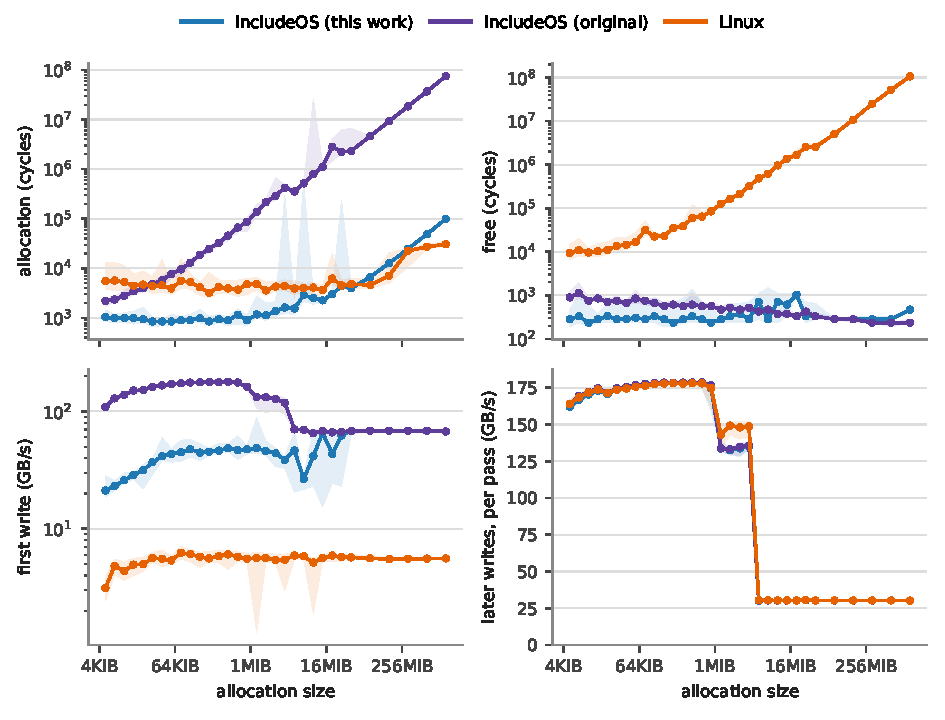
\includegraphics[width=0.92\textwidth]{fig/first-touch-mmap.pdf}
  \caption{What a region from \texttt{mmap} costs once it is used, by region size. Top: cycles spent mapping and unmapping, where a lower line is cheaper. Bottom: how fast the region is written the first time and afterwards, in GB/s, where a higher line is faster. Lines are medians over $n = 30$ boots with five seeds each, and the shaded bands span the 25th to 75th percentile.}
  \label{fig:alloc-first-touch}
\end{figure}

\begin{table}[h]
  \centering
  \small
  \caption{Median cycles to map a region with \texttt{mmap} and write it once, by size, the total price of starting to use new memory: the sum of the two left panels of \cref{fig:alloc-first-touch}, over the same runs. \emph{Ratio} is this work over Linux, so below $1.00\times$ means this work is cheaper. Sizes up to 32\,MiB come from the randomised workload, and 256\,MiB and 1\,GiB from the fixed-size workload.}
  \label{tab:first-touch}
  \colortablesetup
  \setlength{\tabcolsep}{9pt}
  \rowcolors{2}{}{black!5}
  \begin{tabular}{lrrrr}
    \toprule
    size & \rothead{\sysorig{original}} & \rothead{\systhis{this work}}
         & \rothead{\syslinux{Linux}} & ratio \\
    \midrule
    4--8\,KiB & $2.5\cdot10^{3}$ & $2.4\cdot10^{3}$ & $12.9\cdot10^{3}$ & 0.19$\times$ \\
    64--128\,KiB & $14.5\cdot10^{3}$ & $11.2\cdot10^{3}$ & $90.9\cdot10^{3}$ & 0.12$\times$ \\
    1--2\,MiB & $270\cdot10^{3}$ & $173\cdot10^{3}$ & $1.48\cdot10^{6}$ & 0.12$\times$ \\
    4--8\,MiB & $798\cdot10^{3}$ & $933\cdot10^{3}$ & $4.38\cdot10^{6}$ & 0.21$\times$ \\
    16--32\,MiB & $4.41\cdot10^{6}$ & $2.35\cdot10^{6}$ & $24.3\cdot10^{6}$ & 0.097$\times$ \\
    256\,MiB & $36.9\cdot10^{6}$ & $18.5\cdot10^{6}$ & $227\cdot10^{6}$ & 0.081$\times$ \\
    1\,GiB & $150\cdot10^{6}$ & $75.0\cdot10^{6}$ & $902\cdot10^{6}$ & 0.083$\times$ \\
    \bottomrule
  \end{tabular}
\end{table}

Once memory has been written, all three systems write to it at the same speed: about 165--178\,GB/s up to a few hundred KiB, 130--150\,GB/s around 1--2\,MiB, and 30\,GB/s from 4\,MiB up (bottom right of \cref{fig:alloc-first-touch}). What separates them is when they pay for new memory: when it is mapped, when it is first written, or when it is unmapped.

On Linux, most of that cost comes after the mapping. Its \texttt{mmap} costs about 3\,900--5\,600 cycles up to 32\,MiB, and the work comes at the first write, where every 4\,KiB page faults and is zeroed by the kernel on the way, so freshly mapped memory is written at 4--6\,GB/s at every size. Linux then pays again at \texttt{munmap}, which has to tear down every page that was faulted in, and grows from about 10\,000 cycles to 106~million at 1\,GiB.

The original IncludeOS does the opposite, and pays when the memory is mapped. Its \texttt{mmap} zeroes the whole region, so the cost grows with size, to 2.2~million cycles at 16--32\,MiB. After that, nothing faults, and the first write runs at 67--175\,GB/s up to 32\,MiB. Unmapping stays under 1\,000 cycles at every size.

This work keeps the original's cheap unmapping, but drops the zeroing at map time. Its \texttt{mmap} costs about 1\,000 cycles up to 1\,MiB, then grows by about 94 cycles per MiB, probably because applying the requested protection touches more page table entries. It is cheaper than Linux up to 16\,MiB and passes it between 32 and 64\,MiB. At 1\,GiB it takes 98\,900 cycles, against 30\,600 for Linux. The first write runs at 22--62\,GB/s up to 32\,MiB, slower than the original. We reran this work with the \texttt{memset} in \texttt{mmap} put back, and nothing else changed, and its first writes then ran at the original's speed: within a few per cent at every size up to 16\,MiB, except 61 against 70\,GB/s at 4--8\,MiB. We think that is because the zeroing has just written the region and left it in cache, but we did not measure the cache itself. That cannot explain large regions, which do not fit in cache, and from 32\,MiB up the three IncludeOS builds write equally fast.

Added up (\cref{tab:first-touch}), allocating a region and writing it once costs 5--12 times more on Linux than with this work's \texttt{mmap}. That is not a like-for-like comparison, since Linux clears the memory and this work does not. The original IncludeOS clears it too, and Linux still costs 5--6 times more than it at every size, so most of the difference comes from IncludeOS backing its memory at boot, and the rest from skipping the clearing. Against the original IncludeOS, dropping the zeroing halves the total for large regions, but not at every size: at 4--8\,MiB the original is cheaper ($0.80\cdot10^{6}$ against $0.93\cdot10^{6}$ cycles), because its zeroing speeds up the first write.

The custom allocator (\cref{tab:first-touch-custom,tab:first-write-custom}) shows what going through \texttt{mmap} costs at all. Taking a block from a pool it already has costs the buddy allocator about 190 cycles on IncludeOS and 280--1\,200 on Linux, against 1\,000 and 5\,600 cycles for an \texttt{mmap} of the smallest regions. Its first writes still depend on how the pool was backed. On IncludeOS the pool is backed from boot, and the first write runs at 32--70\,GB/s. On Linux the pool was mapped lazily, so a first write is fast only if an earlier allocation already touched that block. Otherwise every page faults and the write runs at about 6\,GB/s (\cref{tab:first-write-custom}). This is the common case: it covers 54\,\% of first writes at 4--8\,KiB and 90\,\% at 16--32\,MiB, probably because large blocks are less often carved from memory that was used before. \Cref{tab:first-write-custom} reports the two cases separately, since a median over both jumps between them from one size to the next.

\begin{table}[h]
  \centering
  \small
  \caption{Allocating without \texttt{mmap}: median cycles for a buddy allocator compiled into the benchmark to hand out one block from a 1\,GiB pool it mapped once at startup, over the runs of \cref{fig:alloc-first-touch}. Fewer cycles mean a faster allocation.}
  \label{tab:first-touch-custom}
  \colortablesetup
  \setlength{\tabcolsep}{9pt}
  \rowcolors{2}{}{black!5}
  \begin{tabular}{lrrr}
    \toprule
    size & \sysorig{original} & \systhis{this work} & \syslinux{Linux} \\
    \midrule
    4--8\,KiB    & 188 & 188 & 517  \\
    64--128\,KiB & 188 & 188 & 752  \\
    1--2\,MiB    & 188 & 235 & 1222 \\
    4--8\,MiB    & 188 & 188 & 705  \\
    16--32\,MiB  & 188 & 188 & 282  \\
    \bottomrule
  \end{tabular}
\end{table}

\begin{table}[h]
  \centering
  \small
  \caption{The first write to a block from the custom allocator of \cref{tab:first-touch-custom}: how fast that write runs, as median GB/s over the same runs, so a page fault shows up as a low number. For Linux, the table gives the share of first writes that page-fault, and the median of the faulting and non-faulting writes separately.}
  \label{tab:first-write-custom}
  \colortablesetup
  \setlength{\tabcolsep}{9pt}
  \rowcolors{1}{}{black!5}
  \begin{tabular}{lrrrrr}
    \hiderowcolors
    \toprule
    & & & \multicolumn{3}{c}{\syslinux{Linux}} \\
    \cmidrule(lr){4-6}
    size & \sysorig{original} & \systhis{this work}
         & faulting & when faulting & when backed \\
    \midrule
    \showrowcolors
    4--8\,KiB    & 32 & 42 & 54\,\% & 8.9 & 21 \\
    64--128\,KiB & 46 & 50 & 56\,\% & 6.4 & 42 \\
    1--2\,MiB    & 47 & 50 & 67\,\% & 6.3 & 50 \\
    4--8\,MiB    & 70 & 70 & 71\,\% & 6.2 & 68 \\
    16--32\,MiB  & 68 & 68 & 90\,\% & 6.1 & 67 \\
    \bottomrule
  \end{tabular}
\end{table}

One thing these measurements leave open is why, on IncludeOS, the first write to a large region is faster than the later ones: 62--68\,GB/s against 30\,GB/s at 16--32\,MiB, for the custom allocator and for this work's \texttt{mmap}. The first write stores zeros and the later ones store a nonzero value, but we have not checked whether that is what makes the difference.

Taken together, eager commit wins by a wide margin for memory that gets used. For memory that is reserved and left alone, lazy commit wins, as the OCaml workload shows (\fullref{sec:eval-ocaml}), since its heap is reserved large and barely touched. A unikernel that knows which kind of allocation it is making could get both, and this is part of what the allocation hints in \Cref{sec:design-mmap} could carry.

\section{OCaml workload}
\label{sec:eval-ocaml}

For \textbf{RQ3}, we run an OCaml program on the new memory interface: a small fiber scheduler built on OCaml~5's algebraic effects. It spawns seven fibers in a binary tree (depth two), runs them round-robin, and exits. The workload is deliberately small, since the point is to exercise the runtime. Timing is taken outside the runtime: \texttt{caml\_startup} and the workload entry point are timed separately, and the fiber scheduler's own source is not instrumented. Memory statistics come from the allocator's \texttt{stats()} on IncludeOS, and from \texttt{/proc/self/maps} and \texttt{getrusage} on Linux.

Both platforms use OCaml~5.3 with the configure flags of \fullref{sec:design-ocaml-build}, with one difference. The IncludeOS build of this workload uses only the two flags IncludeOS needs, \texttt{--disable-systhreads} and the \texttt{sigprocmask} override, while the Linux build also uses \texttt{--enable-mmap-map-stack}, which makes no measurable difference here (\cref{tab:mapstack-kvm}). We also keep a stock Linux build as a reference for what normal OCaml~5.3 performance looks like.

\subsection{Runtime performance}

\begin{table}[h]
  \centering
  \caption{Where an OCaml~5.3 program spends its time: mean RDTSC cycles $\pm$ standard deviation over $n = 30$ runs, where fewer cycles mean the program finishes sooner. \texttt{caml\_startup} sets up the runtime, and \texttt{ocaml\_entry} runs the fiber workload.}
  \label{tab:ocaml-timing}
  \begin{tabular}{lrr}
    \toprule
    & \systhis{IncludeOS} & \syslinux{Linux} \\
    \midrule
    \texttt{caml\_startup} & $200\,000 \pm 33\,000$ & $554\,000 \pm 47\,000$ \\
    \texttt{ocaml\_entry}  & $31\,137\,000 \pm 283\,000$ & $37\,829\,000 \pm 357\,000$ \\
    \bottomrule
  \end{tabular}
\end{table}

IncludeOS is about $2.8\times$ faster than Linux for \texttt{caml\_startup} and $1.2\times$ faster for \texttt{ocaml\_entry} (\cref{tab:ocaml-timing}).

\texttt{caml\_startup} covers everything the OCaml runtime does before the program's own code runs: setting up the garbage collector, running module-level initialisers, reserving the heap, and committing the first domain's minor heap inside it with \texttt{MAP\_FIXED} (\texttt{count\_alloc\_at}~$= 1$ in \cref{tab:ocaml-memory}). Even though Linux here is already virtualised, its kernel's \texttt{mmap} path still goes through virtual memory area (VMA) bookkeeping and signal-handler registration. On IncludeOS, the buddy allocator serves both calls directly without any kernel in the way, which is cheaper.

The startup numbers are noisier than the entry numbers (IncludeOS: $175$--$294\cdot10^{3}$ cycles; Linux: $457$--$642\cdot10^{3}$), with a few slow runs scattered through each batch, so the startup numbers are rough.

\texttt{ocaml\_entry} runs the fiber scheduler itself. The difference is smaller there: both platforms pay for OCaml's effects machinery and GC, and with only seven fiber stacks the per-\texttt{mmap} difference between the buddy allocator and the Linux VMA path is small compared to everything else going on.

As a check, we added and removed \texttt{--enable-mmap-map-stack} on its own, since the Linux build used so far in this section changes all three flags at once and cannot tell us which one matters. We measured the three builds of \cref{tab:mapstack-linux} two ways: natively, pinned to one core, and as in the rest of this section.

\begin{table}[h]
\centering
\caption{The three OCaml builds of \cref{sec:design-ocaml-build} on native Linux without QEMU, pinned to one core (RDTSC cycles, mean $\pm$ standard deviation, $n=30$), so whatever the flag costs shows up as extra cycles. \emph{Stock} has no configure flags, \emph{trimmed} has the two IncludeOS needs, and \emph{matched} adds \texttt{--enable-mmap-map-stack}.}
\label{tab:mapstack-linux}
\begin{tabular}{lrr}
  \toprule
  configuration & \texttt{caml\_startup\_cycles} & \texttt{ocaml\_entry\_cycles} \\
  \midrule
  stock    & $973\,334 \pm 489\,870$ & $157\,459 \pm 79\,013$ \\
  trimmed\textsuperscript{*}  & $902\,011 \pm 281\,068$ & $138\,786 \pm 17\,450$ \\
  matched  & $901\,570 \pm 308\,297$ & $207\,002 \pm 11\,543$ \\
  \bottomrule
\end{tabular}
\end{table}

Natively, adding \texttt{--enable-mmap-map-stack} costs $49.15\,\%$ more \texttt{ocaml\_entry} cycles (\Cref{tab:mapstack-linux}). The difference comes from that flag. \texttt{caml\_startup\_cycles} barely moves between trimmed and matched, since no fiber stacks exist yet at that point; the two only diverge once \texttt{ocaml\_entry} spawns the fiber tree. That tracks with what the flag changes, an \texttt{mmap} call per fiber stack (\fullref{sec:design-ocaml-build}). On Linux that trades a cheap pool-allocator hit for an actual syscall, over and over, for a scheduler that spawns and retires several short-lived fibers.

\begin{table}[h]
\centering
\caption{The same three OCaml builds as \cref{tab:mapstack-linux}, inside QEMU: workload cycles only (\texttt{ocaml\_entry}, mean $\pm$ standard deviation, $n=30$), where a cost of the flag would again show up as extra cycles.}
\label{tab:mapstack-kvm}
\begin{tabular}{lrr}
  \toprule
  configuration & \systhis{IncludeOS} & \syslinux{Linux} \\
  \midrule
  stock\textsuperscript{\dag}    & panics & $56\,407\,862 \pm 653\,994$ \\
  trimmed\textsuperscript{*}  & $31\,111\,507 \pm 455\,693$ & $56\,356\,209 \pm 367\,105$ \\
  matched  & $31\,298\,976 \pm 832\,007$ & $56\,503\,633 \pm 601\,998$ \\
  \bottomrule
\end{tabular}
\end{table}

\textsuperscript{*}Both flags in \emph{trimmed} are necessary on IncludeOS for reasons unrelated to this comparison (\fullref{sec:design-ocaml-build}). \textsuperscript{\dag}Attempted: it panics immediately, with \texttt{Fatal error: Failed to allocate signal stack for domain 0}. Stock flags leave \texttt{POSIX\_SIGNALS} defined, so \texttt{caml\_init\_signals} calls \texttt{sigaltstack}, which IncludeOS does not implement (\fullref{sec:conclusion}).

Measured the usual way, though, the difference disappears on both platforms. \texttt{ocaml\_entry\_cycles} is in the tens of millions here, several hundred times the native numbers. The fiber scheduler prints about two dozen lines per run, each one flushed, and I/O through QEMU usually costs a VM exit per call. That probably drowns out the small allocator difference seen natively, although we have not tested that explanation the way we tested the flag itself. Whatever the cause, \texttt{--enable-mmap-map-stack} changes how fiber stacks are allocated, but under the conditions our comparisons use it makes no measurable difference to performance on either system.

\subsection{Memory usage}

\begin{table}[h]
  \centering
  \caption{Memory used by the OCaml fiber workload. The numbers are identical in all 30 runs, so there is no mean or median.}
  \label{tab:ocaml-memory}
  \begin{tabular}{lrr}
    \toprule
    & \systhis{IncludeOS} & \syslinux{Linux} \\
    \midrule
    peak requested (MiB) & 271.5 & 257.5 \\
    \texttt{count\_alloc\_at}    & 1     & —     \\
    peak RSS (MiB)        & —     & 0.8   \\
    \bottomrule
  \end{tabular}
\end{table}

Both platforms reserve approximately $270\,\text{MiB}$ for the OCaml heap (\cref{tab:ocaml-memory}), but only Linux gets away with backing almost none of it. The small difference ($\approx 14\,\text{MiB}$) is probably alignment rounding: the buddy allocator works in powers of two, so it rounds up to the nearest block boundary.

Peak RSS (resident set size) is how much physical RAM the process used at its peak, as opposed to how much virtual address space it reserved. Only Linux reports it, through \texttt{getrusage(RUSAGE\_SELF)}, since IncludeOS does not track page residency.

Linux commits memory lazily, page by page as the program writes it (\fullref{sssec:posix-memory}), so the reservation costs almost nothing upfront, which is why RSS stays at only $0.8\,\text{MiB}$ despite the large virtual reservation. The low number also reflects that we run a single OCaml binary with no other processes around.

IncludeOS backs all memory at boot. For a workload like this one, which reserves a big arena and touches a small part of it, IncludeOS therefore uses more physical memory than Linux for the same reservation, which contradicts the idea that more control automatically means less memory used. Committing eagerly is not a property of the region model. Nothing about named regions requires it, and a demand-paged strategy could sit behind the same interface. With named regions, the burden shifts onto the caller instead: knowing their own allocation pattern well enough to pick the right region, and when it should be ready.

The remaining row of \cref{tab:ocaml-memory}, \texttt{count\_alloc\_at}, exists only on IncludeOS. It counts calls to the buddy allocator's fixed-address interface, used to implement \texttt{MAP\_FIXED}. Linux has no equivalent counter because the kernel handles this internally and does not expose a per-call count.

The value $1$ is the commit of one domain's minor heap inside the reservation, not the reservation itself (\fullref{sec:design-ocaml}), so for \textbf{RQ3} it shows \texttt{allocate\_at} serving the request OCaml needs. The runtime never calls \texttt{mprotect} itself, on either system: the commit changes the permission through \texttt{mmap} with \texttt{MAP\_FIXED}, which on IncludeOS calls \texttt{\_\_sys\_mprotect} internally, and the Linux traces behind \cref{tab:sandmark-calls}, which also logged \texttt{mprotect}, show none in any Sandmark program.

Every OCaml workload in this chapter, including the Sandmark benchmarks, runs on exactly one domain (\fullref{sec:design-ocaml}), which is why there is exactly one commit.

Both harnesses also report how many allocations the workload made, but the two numbers count different things, and neither appears in \cref{tab:ocaml-memory} for that reason. On IncludeOS, \texttt{count\_alloc} is the number of calls to the buddy allocator since boot: 60 in every run. Linux has no such counter, so its harness counts the anonymous mappings listed in \texttt{/proc/self/maps} when the workload ends instead: 8 or 9.

Most of the 60 are not OCaml's. In a separate run with the counter also read just before OCaml starts, which made 59 calls in total, 55 of them happened while the kernel booted, and 4 while OCaml ran, plus the one fixed-address commit (\cref{tab:ocaml-memory}). On Linux, a mapping that was already unmapped is gone from \texttt{/proc/self/maps}, and the kernel merges neighbouring mappings with the same permissions into one entry, which is why the count varies between runs. Traced with \texttt{strace} instead, the workload makes 24 \texttt{mmap} calls on Linux while OCaml runs. Part of that difference is the fiber stacks, which the Linux build maps one by one, and the rest is musl's \texttt{malloc}, which in this Linux build is \texttt{mallocng} and maps and unmaps small groups of blocks (\fullref{sec:memory-allocation}).

\subsection{Sandmark}
\label{sec:eval-sandmark}

The fiber workload (\fullref{sec:eval-ocaml}) exercises the runtime, but it does very little work. To see how ordinary OCaml programs behave, we also run 18 benchmarks from Sandmark (\fullref{sec:bg-sandmark}). We use the ones that are a single source file and need no external packages: classic algorithmic benchmarks (\texttt{almabench}, \texttt{bdd}, \texttt{hamming}, \texttt{kb}, \texttt{soli}, \texttt{sequence\_cps}), numerical ones (\texttt{dka}, \texttt{crout}, \texttt{qr}), deep recursion (the \texttt{rec\_seq\_*} family), and three small allocation tests (\texttt{alloc}, \texttt{morestacks}, \texttt{lazy\_primes}).

Each benchmark is built three ways: for IncludeOS, for Linux with the same OCaml configure flags, and for Linux with a stock OCaml~5.3. All three run 30 times each. Since OCaml runs a program's top-level code during \texttt{caml\_startup}, we time that call, which covers the runtime's startup and the whole benchmark. Every benchmark runs on IncludeOS and prints the same output as on Linux.

\begin{table}[!htbp]
  \centering
  \small
  \caption{Sandmark programs on IncludeOS and on Linux: mean RDTSC cycles to run the whole program ($n = 30$), with the standard deviation as a share of the mean. \emph{Ratio} is IncludeOS over Linux, so below $1.00\times$ means IncludeOS is faster. Rows are sorted by ratio.}
  \label{tab:sandmark}
  \colortablesetup
  \setlength{\tabcolsep}{8pt}
  \begin{tabular}{llrrrrr}
    \toprule
    benchmark & kind & \rothead{\syslinux{Linux} cycles} & \rothead{sd}
              & \rothead{\systhis{IncludeOS} cycles} & \rothead{sd}
              & \rothead{ratio} \\
\midrule
    \rowcolor{kindalloc}\texttt{morestacks}$^\dagger$ & allocation & $43.4\cdot10^{9}$ & 0.8\,\% & $210\cdot10^{9}$ & 0.4\,\% & 4.83$\times$ \\
    \rowcolor{kindalloc}\texttt{alloc} & allocation & $7.1\cdot10^{9}$ & 0.8\,\% & $22.1\cdot10^{9}$ & 0.4\,\% & 3.11$\times$ \\
    \rowcolor{kindnum}\texttt{crout} & numerical & $2.83\cdot10^{9}$ & 1.5\,\% & $8.63\cdot10^{9}$ & 0.5\,\% & 3.05$\times$ \\
    \rowcolor{kindalg}\texttt{sequence\_cps} & algorithmic & $41.7\cdot10^{6}$ & 0.8\,\% & $126\cdot10^{6}$ & 0.5\,\% & 3.02$\times$ \\
    \rowcolor{kindnum}\texttt{dka} & numerical & $3.26\cdot10^{9}$ & 1.1\,\% & $5.95\cdot10^{9}$ & 0.6\,\% & 1.82$\times$ \\
    \rowcolor{kindnum}\texttt{qr} & numerical & $4.94\cdot10^{9}$ & 0.7\,\% & $8.4\cdot10^{9}$ & 0.4\,\% & 1.70$\times$ \\
    \rowcolor{kindrec}\texttt{rec\_seq\_motzkin} & recursion & $2.63\cdot10^{9}$ & 0.7\,\% & $4.05\cdot10^{9}$ & 0.6\,\% & 1.54$\times$ \\
    \rowcolor{kindalg}\texttt{almabench} & algorithmic & $3.85\cdot10^{9}$ & 1.2\,\% & $5.63\cdot10^{9}$ & 0.5\,\% & 1.46$\times$ \\
    \rowcolor{kindalg}\texttt{hamming} & algorithmic & $202\cdot10^{6}$ & 1.1\,\% & $245\cdot10^{6}$ & 1.1\,\% & 1.22$\times$ \\
    \rowcolor{kindalg}\texttt{kb\_no\_exc} & algorithmic & $4.48\cdot10^{9}$ & 1.0\,\% & $5.23\cdot10^{9}$ & 0.6\,\% & 1.17$\times$ \\
    \rowcolor{kindalloc}\texttt{lazy\_primes} & allocation & $1.27\cdot10^{9}$ & 1.4\,\% & $1.44\cdot10^{9}$ & 0.9\,\% & 1.14$\times$ \\
    \rowcolor{kindalg}\texttt{kb} & algorithmic & $7\cdot10^{9}$ & 0.9\,\% & $7.77\cdot10^{9}$ & 1.0\,\% & 1.11$\times$ \\
    \rowcolor{kindrec}\texttt{rec\_seq\_fib} & recursion & $6.11\cdot10^{9}$ & 1.0\,\% & $6.46\cdot10^{9}$ & 1.1\,\% & 1.06$\times$ \\
    \rowcolor{kindrec}\texttt{rec\_seq\_ack} & recursion & $1.42\cdot10^{9}$ & 1.2\,\% & $1.42\cdot10^{9}$ & 1.1\,\% & 1.00$\times$ \\
    \rowcolor{kindrec}\texttt{rec\_seq\_tak} & recursion & $3.74\cdot10^{9}$ & 0.9\,\% & $3.7\cdot10^{9}$ & 1.0\,\% & 0.99$\times$ \\
    \rowcolor{kindrec}\texttt{rec\_seq\_sudan} & recursion & $2.5\cdot10^{9}$ & 0.9\,\% & $2.48\cdot10^{9}$ & 1.0\,\% & 0.99$\times$ \\
    \rowcolor{kindalg}\texttt{bdd} & algorithmic & $566\cdot10^{6}$ & 2.3\,\% & $534\cdot10^{6}$ & 1.1\,\% & 0.94$\times$ \\
    \rowcolor{kindalg}\texttt{soli} & algorithmic & $20\cdot10^{6}$ & 0.8\,\% & $16.2\cdot10^{6}$ & 2.2\,\% & 0.81$\times$ \\
    \bottomrule
  \end{tabular}

  \vspace{4pt}
  \raggedright\footnotesize
  $^\dagger$ Two of the 30 IncludeOS runs hung at shutdown and are left out.
\end{table}

\begin{table}[!htbp]
  \centering
  \small
  \caption{How often each program of \cref{tab:sandmark} asks for memory during \texttt{caml\_startup}: calls to the IncludeOS allocator, and Linux system calls traced with \texttt{strace}, with both using musl's \texttt{oldmalloc}. One run per program, since the counts do not vary between runs. \texttt{FIXED} is \texttt{mmap} with \texttt{MAP\_FIXED}, left out of the \texttt{mmap} column.}
  \label{tab:sandmark-calls}
  \colortablesetup
  \setlength{\tabcolsep}{4pt}
  \begin{tabular}{lrrrrrrr}
    \toprule
    & \multicolumn{3}{c}{\systhis{IncludeOS} allocator}
    & \multicolumn{4}{c}{\syslinux{Linux} system calls} \\
    \cmidrule(lr){2-4}\cmidrule(lr){5-8}
    benchmark & \texttt{allocate} & \texttt{\_at} & \texttt{dealloc.}
              & \texttt{mmap} & \texttt{FIXED} & \texttt{munmap} & \texttt{brk} \\
    \midrule
    \rowcolor{kindalloc}\texttt{morestacks} & 5 & 1 & 0 & 5 & 1 & 0 & 9 \\
    \rowcolor{kindalloc}\texttt{alloc} & 8 & 1 & 0 & 9 & 1 & 0 & 9 \\
    \rowcolor{kindnum}\texttt{crout} & 81 & 1 & 0 & 75 & 1 & 0 & 2745 \\
    \rowcolor{kindalg}\texttt{sequence\_cps} & 14 & 1 & 0 & 15 & 1 & 0 & 9 \\
    \rowcolor{kindnum}\texttt{dka} & 33 & 1 & 0 & 33 & 1 & 0 & 9 \\
    \rowcolor{kindnum}\texttt{qr} & 20 & 1 & 0 & 20$^\ddagger$ & 1 & 0 & 810 \\
    \rowcolor{kindrec}\texttt{rec\_seq\_motzkin} & 17 & 1 & 0 & 18 & 1 & 0 & 9 \\
    \rowcolor{kindalg}\texttt{almabench} & 15 & 1 & 0 & 15 & 1 & 0 & 9 \\
    \rowcolor{kindalg}\texttt{hamming} & 858 & 1 & 0 & 841 & 1 & 0 & 9 \\
    \rowcolor{kindalg}\texttt{kb\_no\_exc} & 173 & 1 & 3 & 177 & 1 & 3 & 9 \\
    \rowcolor{kindalloc}\texttt{lazy\_primes} & 3952 & 1 & 3 & 3919 & 1 & 3 & 9 \\
    \rowcolor{kindalg}\texttt{kb} & 171 & 1 & 3 & 174 & 1 & 3 & 9 \\
    \rowcolor{kindrec}\texttt{rec\_seq\_fib} & 5 & 1 & 0 & 5 & 1 & 0 & 9 \\
    \rowcolor{kindrec}\texttt{rec\_seq\_ack} & 9 & 1 & 4 & 9 & 1 & 4 & 9 \\
    \rowcolor{kindrec}\texttt{rec\_seq\_tak} & 5 & 1 & 0 & 5 & 1 & 0 & 9 \\
    \rowcolor{kindrec}\texttt{rec\_seq\_sudan} & 5 & 1 & 0 & 5 & 1 & 0 & 9 \\
    \rowcolor{kindalg}\texttt{bdd} & 114 & 1 & 0 & 116$^\ddagger$ & 1 & 0 & 25 \\
    \rowcolor{kindalg}\texttt{soli} & 5 & 1 & 0 & 5 & 1 & 0 & 9 \\
    \bottomrule
  \end{tabular}

  \vspace{4pt}
  \raggedright\footnotesize
  $^\ddagger$ Plus a few \texttt{madvise} calls (2 for \texttt{bdd}, 3 for \texttt{qr}).
\end{table}

The results fall into four groups (\cref{tab:sandmark}). Three of the five \texttt{rec\_seq\_*} benchmarks run at the same speed on both platforms, within 5\,\%. \texttt{bdd} and \texttt{soli} are 6 and 19\,\% faster on IncludeOS. Nine are 6--82\,\% slower, and four are three to five times slower: \texttt{morestacks}, \texttt{alloc}, \texttt{crout}, and \texttt{sequence\_cps}. Medians are within 1\,\% of the means for every program. \texttt{morestacks} and \texttt{alloc} are allocation tests by design, yet they barely ask the operating system for memory (\cref{tab:sandmark-calls}). \texttt{morestacks} makes five allocator calls on IncludeOS, as many as the recursion benchmarks that run at Linux speed, and \texttt{lazy\_primes} makes 3\,952, the most of any program, but is only 14\,\% slower. The OCaml runtime takes one large heap at startup and manages it itself, so how much a program allocates barely shows up as calls, on either system.

Since both systems use the same \texttt{malloc} from musl, \texttt{oldmalloc} (\fullref{sec:memory-allocation}), they make about the same calls for the same program. Linux's \texttt{munmap} calls match IncludeOS' frees exactly, and its \texttt{mmap} calls come close to IncludeOS' allocations. Following each \texttt{mmap} back to the function that called it shows that musl's \texttt{malloc} makes exactly two of them in every program, and the OCaml runtime makes the rest, mostly as it grows its heap. Both systems make exactly one fixed-address commit, for OCaml's minor heap, as in the fiber workload. Linux also calls \texttt{brk}, which the IncludeOS columns do not count, since IncludeOS serves it from its own fixed area.

The calls in \cref{tab:sandmark-calls} were counted in separate runs, outside the timed ones. On IncludeOS, the allocator counts the calls it receives (\texttt{count\_alloc}, \texttt{count\_alloc\_at} and \texttt{count\_dealloc}), and the benchmark reads them right before and right after \texttt{caml\_startup}, so the table only counts what happens while OCaml runs. The timed runs print the same counters once, as totals since boot, and they add up to the same numbers.

On Linux, we ran the programs natively under \texttt{strace -f}, logging every \texttt{mmap}, \texttt{munmap}, \texttt{mremap}, \texttt{mprotect} and \texttt{brk}, and counted the calls between the two lines the program prints before and after \texttt{caml\_startup}.
% counts: see sandmark/ in msc-thesis-benchmarks
To see where the time goes, we sampled the guest's instruction pointer while \texttt{alloc} ran on IncludeOS (\fullref{sec:eval-methodology}). Nearly every sample lands in the benchmark's own compiled OCaml code, in the loop that allocates small blocks by bumping a pointer into the minor heap and writing them. None land in IncludeOS' allocator, in \texttt{mmap}, or in musl's \texttt{malloc}. Most of them sit on the load that checks the minor heap's limit, right after the stores into it. The same load runs in the \texttt{rec\_seq\_*} benchmarks without those stores, and they run at Linux speed. The cost is thus in how memory behaves under IncludeOS for this store-heavy code, and the calls the runtime makes to IncludeOS play no part in it (\fullref{sec:discussion-results} discusses what might cause it).

The two Linux builds are within 1\,\% of each other on every benchmark, so the configure flags we need for IncludeOS do not change OCaml's performance on Linux.

\section{Zig Feasibility}
\label{sec:eval-zig-feasibility}

None of the timings for \textbf{RQ5}, whether POSIX is needed at all, mean anything unless two things hold: a Zig object file can be compiled separately and linked into an IncludeOS unikernel, and Zig code can use \texttt{os::mem::raw\_allocator()} correctly. We check both in a separate, minimal repository, \texttt{zig-hello-world}, with nothing benchmark-related in it. It exports two functions. \texttt{zig\_add} is a trivial FFI check: it adds two integers in Zig and returns the result to C++, which prints \texttt{zig\_add(2, 40) = 42} at boot, so values survive the C ABI boundary in both directions.

The second function, \texttt{zig\_alloc\_roundtrip}, tests the allocator path. It allocates 64 \texttt{u32}s through a \texttt{std.mem.Allocator} backed by \texttt{os::mem::raw\_allocator()}, fills each with the square of its index ($i^2$), and checks every element reads back correctly. Then it reallocates the buffer to 256 elements, which forces Zig through its alloc-copy-free fallback, worth testing by itself. It then checks that the original 64 values survived the copy, and frees the buffer. Each step that can fail has a distinct negative return code, and the function returns \texttt{0} only if everything worked. Booted on IncludeOS, the service prints \texttt{zig\_alloc\_roundtrip() = 0}, with a message that every step passed. Both functions succeed, so the toolchain link works (Zig's compiler, IncludeOS' musl and C++ runtime, and the C ABI between them), and so does the allocator path, before any performance comparison starts.

The allocator path crosses languages through a small shim (\cref{fig:zig-allocator-path}). Zig's \texttt{std.mem.Allocator} vtable is backed by two \texttt{extern} functions, \texttt{includeos\_zig\_alloc} and \texttt{includeos\_zig\_free}, in a thin C++ shim that calls \texttt{os::\allowbreak mem::\allowbreak raw\_allocator()}'s \texttt{allocate}/\texttt{deallocate}. The shim's only job is to contain C++ exceptions. If \texttt{allocate} runs out of memory or overbooks, it throws, and that exception must never cross the \texttt{extern "C"} boundary. Zig has no exceptions. Errors are ordinary return values, in error union types \cite[Errors]{zig-langref}, so nothing on the Zig side could handle a C++ exception. The shim catches it and returns \texttt{nullptr}.

On the Zig side, \texttt{resize} and \texttt{remap} are wired to Zig's built-in \texttt{noResize}/\texttt{noRemap} no-ops rather than to anything IncludeOS-specific, which is why \texttt{realloc} above falls back to alloc-copy-free. The vtable never offers the allocator a chance to grow in place.

\section{Allocation Latency: POSIX vs.\ Direct}
\label{sec:eval-posix-direct}

For \textbf{RQ5}, we time the same allocations two ways: through \texttt{mmap}, and straight through \texttt{os::\allowbreak mem::\allowbreak raw\_allocator()}. We do it in pure C++ first, then again with Zig calling both paths through \texttt{std.mem.Allocator}, to make sure the result comes from the allocator paths and not from the language calling them.

\begin{table}[h]
  \centering
  \caption{The cost of allocating and freeing one block from C++ on IncludeOS, either through \texttt{mmap} (\emph{posix}) or by calling \texttt{os::mem::raw\_allocator()} directly (\emph{direct}). Mean RDTSC cycles per call ($n = 30$ boots, batched workload, after dropping any boot more than three times slower than the median). The ratio is direct over posix, so below $1.00\times$ means skipping POSIX is faster.}
  \label{tab:cpp-posix-direct}
  \colortablesetup
  \rowcolors{1}{}{black!5}
  \begin{tabular}{rrrrrrr}
    \hiderowcolors
    \toprule
    & \multicolumn{3}{c}{alloc} & \multicolumn{3}{c}{free} \\
    \cmidrule(lr){2-4}\cmidrule(lr){5-7}
    size & \pathposix{posix} & \pathdirect{direct} & ratio & \pathposix{posix} & \pathdirect{direct} & ratio \\
    \midrule
    \showrowcolors
    64\,B      &  725 &  176 & 0.24$\times$ & 182 & 163 & 0.90$\times$ \\
    1\,KiB     &  723 &  176 & 0.24$\times$ & 181 & 162 & 0.90$\times$ \\
    4\,KiB     &  724 &  177 & 0.24$\times$ & 184 & 169 & 0.92$\times$ \\
    16\,KiB    & 1108 &  587 & 0.53$\times$ & 177 & 164 & 0.93$\times$ \\
    64\,KiB    & 1937 & 1401 & 0.72$\times$ & 192 & 168 & 0.88$\times$ \\
    256\,KiB   & 6377 & 5779 & 0.91$\times$ & 206 & 177 & 0.86$\times$ \\
    1\,MiB     & 6444 & 5848 & 0.91$\times$ & 264 & 175 & 0.66$\times$ \\
    \bottomrule
  \end{tabular}
\end{table}

\begin{table}[h]
  \centering
  \caption{The same measurement as \cref{tab:cpp-posix-direct} from Zig instead of C++, with both paths reached through \texttt{std.mem.Allocator}.}
  \label{tab:zig-posix-direct}
  \colortablesetup
  \rowcolors{1}{}{black!5}
  \begin{tabular}{rrrrrrr}
    \hiderowcolors
    \toprule
    & \multicolumn{3}{c}{alloc} & \multicolumn{3}{c}{free} \\
    \cmidrule(lr){2-4}\cmidrule(lr){5-7}
    size & \pathposix{posix} & \pathdirect{direct} & ratio & \pathposix{posix} & \pathdirect{direct} & ratio \\
    \midrule
    \showrowcolors
    64\,B      &  775 &  228 & 0.29$\times$ & 234 & 223 & 0.95$\times$ \\
    1\,KiB     &  771 &  226 & 0.29$\times$ & 232 & 223 & 0.96$\times$ \\
    4\,KiB     &  774 &  226 & 0.29$\times$ & 234 & 221 & 0.94$\times$ \\
    16\,KiB    & 1154 &  617 & 0.53$\times$ & 224 & 212 & 0.95$\times$ \\
    64\,KiB    & 1998 & 1455 & 0.73$\times$ & 240 & 223 & 0.93$\times$ \\
    256\,KiB   & 6475 & 5882 & 0.91$\times$ & 259 & 230 & 0.89$\times$ \\
    1\,MiB     & 6441 & 5903 & 0.92$\times$ & 307 & 223 & 0.73$\times$ \\
    \bottomrule
  \end{tabular}
\end{table}

\begin{figure}[tbp]
\centering
\definecolor{seriescpp}{HTML}{2A78D6}
\definecolor{seriesziglang}{HTML}{EB6834}
\begin{tikzpicture}
\begin{groupplot}[
  group style={group size=2 by 1, horizontal sep=1.6cm},
  width=6.6cm, height=4.6cm,
  xmode=log, log basis x=2,
  xtick={64,1024,4096,16384,65536,262144,1048576},
  xticklabels={64B,1KiB,4KiB,16KiB,64KiB,256KiB,1MiB},
  x tick label style={rotate=45, anchor=north east, font=\scriptsize},
  y tick label style={font=\scriptsize},
  xlabel style={font=\scriptsize}, ylabel style={font=\scriptsize},
  ymin=0, ymax=1.1,
  grid=major, grid style={gray!20, thin},
  axis line style={gray!60},
  tick style={gray!60},
  every axis plot/.append style={line width=1pt, mark size=1.4pt},
  legend style={font=\scriptsize, draw=none, fill=none, at={(0.98,0.02)}, anchor=south east},
]

\nextgroupplot[title={(a) alloc}, title style={font=\scriptsize}, ylabel={direct / posix ratio}]
\addplot[color=seriescpp, mark=*] coordinates {
  (64,0.24) (1024,0.24) (4096,0.24) (16384,0.53) (65536,0.72) (262144,0.91) (1048576,0.91)
};
\addplot[color=seriesziglang, mark=square*] coordinates {
  (64,0.29) (1024,0.29) (4096,0.29) (16384,0.53) (65536,0.73) (262144,0.91) (1048576,0.92)
};
\legend{C++, Zig}

\nextgroupplot[title={(b) free}, title style={font=\scriptsize}, ymin=0.6, ymax=1.05]
\addplot[color=seriescpp, mark=*] coordinates {
  (64,0.90) (1024,0.90) (4096,0.92) (16384,0.93) (65536,0.88) (262144,0.86) (1048576,0.66)
};
\addplot[color=seriesziglang, mark=square*] coordinates {
  (64,0.95) (1024,0.96) (4096,0.94) (16384,0.95) (65536,0.93) (262144,0.89) (1048576,0.73)
};

\end{groupplot}
\end{tikzpicture}
\caption{Cycles calling the allocator directly divided by cycles
  through \texttt{mmap} on IncludeOS, by block size, for allocating (a)
  and freeing (b), from C++ and from Zig. Below 1 means the direct path
  is faster. Each point is a ratio of mean cycles over $n = 30$ boots, after
  dropping any boot more than three times slower than the median. Data in
  \cref{tab:cpp-posix-direct,tab:zig-posix-direct}.}
\label{fig:posix-direct-ratio}
\end{figure}


In \cref{fig:posix-direct-ratio}, the C++ and Zig lines follow the same curve. Allocating through \texttt{direct} is faster than through \texttt{posix} at every size, in C++ and in Zig, and the lines never cross: $4.1\times$ and $3.4\times$ faster at 64\,B, narrowing to $1.1\times$ by 256\,KiB--1\,MiB, as \texttt{mmap}'s fixed per-call cost becomes a smaller part of a growing total. Deallocation keeps that ordering, with a smaller and flatter difference ($1.05$--$1.5\times$), which fits \texttt{free} being mostly fixed bookkeeping that does not grow with block size. Since the pattern holds whichever language calls, the advantage comes from the allocator paths. For code that brings its own allocator, POSIX can thus be skipped (\textbf{RQ5}), and skipping it is faster at every size we tested, even the large ones where call overhead should matter least. For memory use, as opposed to speed, \fullref{sec:eval-ocaml} found the opposite (\fullref{sec:conclusion} weighs the two together).

At 64\,B, the \texttt{direct} column of \cref{tab:cpp-posix-direct} reads 176 cycles for C++; the matching column of \cref{tab:zig-posix-direct} reads 228 for Zig: a $1.30\times$ difference with the same hardware, allocator, and workload. In the disassembly, every timed \texttt{allocator.alloc()}\slash\texttt{.free()} call in the Zig loop is an indirect call through \texttt{std.mem.Allocator}'s vtable pointer (\texttt{call *(\%rax)} for allocation, \texttt{call *0x18(\%rax)} for deallocation). The C++ version is a template, compiled separately for each allocator, so its call is a direct call to a fixed address. But Zig and C++ use different compilers with different flags, so some of the difference could come from codegen we cannot see, and not from the vtable. (One difference we can name is that the C++ build has stack-protector instrumentation and the Zig build does not. If anything, that should make C++ the slower one, but it does not rule out other differences.)

To check whether the vtable is the cause, we can mark the allocator parameter \texttt{comptime}, which makes Zig specialise the function per caller, like the C++ template does. The object file's relocations confirm that the indirect calls become direct ones, and the compiler and flags stay the same. If the vtable were not part of the cause, this one change should not move the numbers. \cref{tab:comptime-ratio} shows that it does.

\begin{table}[h]
  \centering
  \caption{Zig's mean cycles over C++'s on the direct path, before and after marking the allocator parameter \texttt{comptime} (batched workload, $n = 30$ boots each, after dropping any boot more than three times slower than the median). $1.00\times$ means Zig is as fast as C++, and anything above it is Zig's overhead.}
  \label{tab:comptime-ratio}
  \colortablesetup
  \rowcolors{1}{}{black!5}
  \begin{tabular}{rrrrr}
    \hiderowcolors
    \toprule
    & \multicolumn{2}{c}{alloc} & \multicolumn{2}{c}{free} \\
    \cmidrule(lr){2-3}\cmidrule(lr){4-5}
    size & \sysorig{no \texttt{comptime}} & \systhis{\texttt{comptime}} & \sysorig{no \texttt{comptime}} & \systhis{\texttt{comptime}} \\
    \midrule
    \showrowcolors
    64\,B      & 1.30$\times$ & 0.96$\times$ & 1.37$\times$ & 1.05$\times$ \\
    1\,KiB     & 1.29$\times$ & 1.01$\times$ & 1.38$\times$ & 1.09$\times$ \\
    4\,KiB     & 1.28$\times$ & 1.00$\times$ & 1.31$\times$ & 1.10$\times$ \\
    16\,KiB    & 1.05$\times$ & 1.01$\times$ & 1.29$\times$ & 1.06$\times$ \\
    64\,KiB    & 1.04$\times$ & 0.99$\times$ & 1.33$\times$ & 1.01$\times$ \\
    256\,KiB   & 1.02$\times$ & 1.00$\times$ & 1.30$\times$ & 1.03$\times$ \\
    1\,MiB     & 1.01$\times$ & 1.00$\times$ & 1.27$\times$ & 1.00$\times$ \\
    \bottomrule
  \end{tabular}
\end{table}

\begin{figure}[tbp]
\centering
\definecolor{seriesnocomptime}{HTML}{2A78D6}
\definecolor{seriescomptime}{HTML}{EB6834}
\begin{tikzpicture}
\begin{groupplot}[
  group style={group size=2 by 1, horizontal sep=1.6cm},
  width=6.6cm, height=4.6cm,
  xmode=log, log basis x=2,
  xtick={64,1024,4096,16384,65536,262144,1048576},
  xticklabels={64B,1KiB,4KiB,16KiB,64KiB,256KiB,1MiB},
  x tick label style={rotate=45, anchor=north east, font=\scriptsize},
  y tick label style={font=\scriptsize},
  xlabel style={font=\scriptsize}, ylabel style={font=\scriptsize},
  grid=major, grid style={gray!20, thin},
  axis line style={gray!60},
  tick style={gray!60},
  every axis plot/.append style={line width=1pt, mark size=1.4pt},
  legend style={font=\scriptsize, draw=none, fill=none, at={(0.98,0.98)}, anchor=north east},
]

\nextgroupplot[title={(a) alloc}, title style={font=\scriptsize},
  ylabel={Zig / C++ ratio}, ymin=0.9, ymax=1.35]
\addplot[color=seriesnocomptime, mark=*] coordinates {
  (64,1.30) (1024,1.29) (4096,1.28) (16384,1.05) (65536,1.04) (262144,1.02) (1048576,1.01)
};
\addplot[color=seriescomptime, mark=square*] coordinates {
  (64,0.96) (1024,1.01) (4096,1.00) (16384,1.01) (65536,0.99) (262144,1.00) (1048576,1.00)
};
\addplot[color=gray, dashed, mark=none, line width=0.5pt] coordinates {(64,1.0) (1048576,1.0)};
\legend{no \texttt{comptime}, \texttt{comptime}}

\nextgroupplot[title={(b) free}, title style={font=\scriptsize}, ymin=0.9, ymax=1.45]
\addplot[color=seriesnocomptime, mark=*] coordinates {
  (64,1.37) (1024,1.38) (4096,1.31) (16384,1.29) (65536,1.33) (262144,1.30) (1048576,1.27)
};
\addplot[color=seriescomptime, mark=square*] coordinates {
  (64,1.05) (1024,1.09) (4096,1.10) (16384,1.06) (65536,1.01) (262144,1.03) (1048576,1.00)
};
\addplot[color=gray, dashed, mark=none, line width=0.5pt] coordinates {(64,1.0) (1048576,1.0)};

\end{groupplot}
\end{tikzpicture}
\caption{Zig's cycles over C++'s on the \texttt{direct} path, by block
  size, for allocating (a) and freeing (b), before and after marking the
  allocator parameter \texttt{comptime}. The dashed line at $1.00\times$
  is C++ speed, and the height above it is Zig's overhead. Each point is a ratio of mean cycles over $n = 30$ boots,
  after dropping any boot more than three times slower than the median.
  Data in \cref{tab:comptime-ratio}.}
\label{fig:comptime-ratio}
\end{figure}


Allocation and deallocation respond differently to it (\cref{fig:comptime-ratio}). Without \texttt{comptime}, the allocation overhead is $30\%$ at small sizes and shrinks as size grows, since a roughly fixed per-call cost matters less and less. With \texttt{comptime}, it drops to noise ($0.96$--$1.01\times$) at every size. Without \texttt{comptime}, the deallocation overhead instead stays roughly flat ($27$--$38\%$), since \texttt{free()} is mostly fixed bookkeeping. With \texttt{comptime}, it shrinks a lot, but settles around $1$--$10\%$ instead of disappearing. The two builds use the same compiler and flags, and differ in whether the allocator is called through the vtable or directly, so we attribute the allocation overhead, and most of the deallocation overhead, to the indirect call. We do not know where the small remaining overhead on \texttt{free} comes from, and leave it open (\fullref{sec:conclusion}).

That answers the question left open in \fullref{sec:design-zig}. That allocator can sit behind a modern, ergonomic interface (an ordinary function parameter) without a measurable cost on allocation, as long as the language can specialise the call site. The idea is older than Zig: C++'s STL allocator template parameter goes back to Stepanov's original design~\cite{stepanov-stl-history}, and D and Rust have similar interfaces (\fullref{sec:allocator-vexation}). Zig makes it the normal way to write any function that allocates, and has \texttt{comptime} as a language feature for removing the abstraction's cost. The interface that made it trivial to switch from \texttt{posix} to \texttt{direct} also makes it trivial to specialise per call site.

\section{Arena vs.\ Buddy}
\label{sec:eval-arena}

The \textbf{RQ6} experiment uses the setup from \fullref{sec:design-arena}: an arena and the buddy allocator, run on the same synthetic scratch workload. There are 50 rounds. Each makes 2 to 5 allocations of 64\,B, 512\,B, 4\,KiB, or 16\,KiB, and frees them all at once with \texttt{deallocate\_all()} before the next round. Every configuration below uses one seed, so all runs see the same sequence of sizes.

\begin{table}[h]
  \centering
  \caption{Peak memory the same scratch workload needs from a buddy allocator and from an arena, each carved from the secondary heap, where a smaller peak leaves more of the heap for everything else. One run with a fixed seed: the allocators have no randomness, so every run gives these numbers exactly, and there is no mean or median.}
  \label{tab:arena-vs-buddy}
  \begin{tabular}{lr}
    \toprule
    allocator & peak used \\
    \midrule
    buddy (standalone) & 48.00\,KiB \\
    arena (standalone) & 44.00\,KiB \\
    \bottomrule
  \end{tabular}
\end{table}

The arena needs 4\,KiB less peak memory than buddy for the same access pattern (44 against 48\,KiB, \cref{tab:arena-vs-buddy}). Since the two get identical sizes, the difference comes from buddy rounding each request up to a power of two. The arena's tight packing depends on freeing everything at once, which a workload that frees in arbitrary order cannot do. Still, the choice of strategy for a region has a measurable cost when the general-purpose one does not fit the access pattern.

Peak memory does not show every way buddy is limited, and it says nothing about \texttt{ring\_resource} (\fullref{sec:allocator-integration}), our third strategy.

The ring allocator is built for the FIFO-like, short-lived allocations a network stack produces, and a quick illustration shows why that matters. A synthetic packet workload (a producer creating many short-lived buffers of varying size, a consumer holding a bounded window of them and releasing each in turn) runs twice. Once with the buddy heap holding the temporary buffers itself, and once with \texttt{ring\_resource} holding them, so the buddy heap only keeps the small, durable record each packet leaves behind. \cref{fig:fragmentation-color-fragmented,fig:fragmentation-color-unfragmented} show the resulting tile maps. Alone, the buddy heap ends up interleaved with many small blocks of different orders, at a block fragmentation of $86.67\%$ (free blocks present, compared with the fewest blocks that much free space could fit in). With the temporary buffers moved to ring, the buddy heap stays fully coalesced into the few large blocks its durable records need, with zero fragmentation.

\begin{figure}[htb]
\centering
\begin{minipage}[t]{0.32\linewidth}
  \small
  \scriptsize
\setlength{\tabcolsep}{2pt}
\renewcommand{\arraystretch}{1.05}
\begin{tabular}{@{}l l@{}}
\definecolor{c0_255_0}{RGB}{0,255,0}
\colorbox{c0_255_0}{\phantom{Xg}} & \texttt{19}: 512.00 KiB (1) \\
\definecolor{c255_0_0}{RGB}{255,0,0}
\colorbox{c255_0_0}{\phantom{Xg}} & \texttt{16}: 64.00 KiB (2) \\
\definecolor{c215_135_0}{RGB}{215,135,0}
\colorbox{c215_135_0}{\phantom{Xg}} & \texttt{15}: 32.00 KiB (4) \\
\definecolor{c255_95_175}{RGB}{255,95,175}
\colorbox{c255_95_175}{\phantom{Xg}} & \texttt{14}: 16.00 KiB (12) \\
\definecolor{c135_0_255}{RGB}{135,0,255}
\colorbox{c135_0_255}{\phantom{Xg}} & \texttt{13}: 8.00 KiB (4) \\
\definecolor{c0_95_255}{RGB}{0,95,255}
\colorbox{c0_95_255}{\phantom{Xg}} & \texttt{12}: 4.00 KiB (13) \\
\definecolor{c135_255_0}{RGB}{135,255,0}
\colorbox{c135_255_0}{\phantom{Xg}} & \texttt{10}: 1.00 KiB (3) \\
\definecolor{c255_175_0}{RGB}{255,175,0}
\colorbox{c255_175_0}{\phantom{Xg}} & \texttt{9}: 512 B (6) \\
\definecolor{c175_0_255}{RGB}{175,0,255}
\colorbox{c175_0_255}{\phantom{Xg}} & \texttt{6}: 64 B (15) \\
\end{tabular}
\end{minipage}%
\begin{minipage}[t]{0.66\linewidth}
  \centering
    \definecolor{c88_88_88}{RGB}{88,88,88}
  \definecolor{c0_95_255}{RGB}{0,95,255}
  \definecolor{c255_95_175}{RGB}{255,95,175}
  \definecolor{c215_135_0}{RGB}{215,135,0}
  \definecolor{c135_255_0}{RGB}{135,255,0}
  \definecolor{c135_0_255}{RGB}{135,0,255}
  \definecolor{c255_0_0}{RGB}{255,0,0}
  \definecolor{c0_255_0}{RGB}{0,255,0}
\begin{tikzpicture}[x=0.14cm, y=0.14cm]
  \path (0,0) rectangle (64,16);
  \fill[c88_88_88] (0,15) rectangle (1,16);
  \fill[c88_88_88] (1,15) rectangle (2,16);
  \fill[c88_88_88] (2,15) rectangle (3,16);
  \fill[c88_88_88] (3,15) rectangle (4,16);
  \fill[c88_88_88] (4,15) rectangle (5,16);
  \fill[c88_88_88] (5,15) rectangle (6,16);
  \fill[c88_88_88] (6,15) rectangle (7,16);
  \fill[c88_88_88] (7,15) rectangle (8,16);
  \fill[c88_88_88] (8,15) rectangle (9,16);
  \fill[c88_88_88] (9,15) rectangle (10,16);
  \fill[c88_88_88] (10,15) rectangle (11,16);
  \fill[c88_88_88] (11,15) rectangle (12,16);
  \fill[c88_88_88] (12,15) rectangle (13,16);
  \fill[c88_88_88] (13,15) rectangle (14,16);
  \fill[c88_88_88] (14,15) rectangle (15,16);
  \fill[c88_88_88] (15,15) rectangle (16,16);
  \fill[c88_88_88] (16,15) rectangle (17,16);
  \fill[c88_88_88] (17,15) rectangle (18,16);
  \fill[c88_88_88] (18,15) rectangle (19,16);
  \fill[c88_88_88] (19,15) rectangle (20,16);
  \fill[c88_88_88] (20,15) rectangle (21,16);
  \fill[c88_88_88] (21,15) rectangle (22,16);
  \fill[c88_88_88] (22,15) rectangle (23,16);
  \fill[c88_88_88] (23,15) rectangle (24,16);
  \fill[c88_88_88] (24,15) rectangle (25,16);
  \fill[c88_88_88] (25,15) rectangle (26,16);
  \fill[c88_88_88] (26,15) rectangle (27,16);
  \fill[c88_88_88] (27,15) rectangle (28,16);
  \fill[c88_88_88] (28,15) rectangle (29,16);
  \fill[c88_88_88] (29,15) rectangle (30,16);
  \fill[c88_88_88] (30,15) rectangle (31,16);
  \fill[c88_88_88] (31,15) rectangle (32,16);
  \fill[c88_88_88] (32,15) rectangle (33,16);
  \fill[c88_88_88] (33,15) rectangle (34,16);
  \fill[c88_88_88] (34,15) rectangle (35,16);
  \fill[c88_88_88] (35,15) rectangle (36,16);
  \fill[c88_88_88] (36,15) rectangle (37,16);
  \fill[c88_88_88] (37,15) rectangle (38,16);
  \fill[c88_88_88] (38,15) rectangle (39,16);
  \fill[c88_88_88] (39,15) rectangle (40,16);
  \fill[c88_88_88] (40,15) rectangle (41,16);
  \fill[c88_88_88] (41,15) rectangle (42,16);
  \fill[c0_95_255] (42,15) rectangle (43,16);
  \fill[c0_95_255] (43,15) rectangle (44,16);
  \fill[c88_88_88] (44,15) rectangle (45,16);
  \fill[c88_88_88] (45,15) rectangle (46,16);
  \fill[c88_88_88] (46,15) rectangle (47,16);
  \fill[c88_88_88] (47,15) rectangle (48,16);
  \fill[c88_88_88] (48,15) rectangle (49,16);
  \fill[c88_88_88] (49,15) rectangle (50,16);
  \fill[c88_88_88] (50,15) rectangle (51,16);
  \fill[c88_88_88] (51,15) rectangle (52,16);
  \fill[c88_88_88] (52,15) rectangle (53,16);
  \fill[c88_88_88] (53,15) rectangle (54,16);
  \fill[c88_88_88] (54,15) rectangle (55,16);
  \fill[c88_88_88] (55,15) rectangle (56,16);
  \fill[c88_88_88] (56,15) rectangle (57,16);
  \fill[c88_88_88] (57,15) rectangle (58,16);
  \fill[c88_88_88] (58,15) rectangle (59,16);
  \fill[c88_88_88] (59,15) rectangle (60,16);
  \fill[c88_88_88] (60,15) rectangle (61,16);
  \fill[c88_88_88] (61,15) rectangle (62,16);
  \fill[c88_88_88] (62,15) rectangle (63,16);
  \fill[c88_88_88] (63,15) rectangle (64,16);
  \fill[c255_95_175] (0,14) rectangle (1,15);
  \fill[c255_95_175] (1,14) rectangle (2,15);
  \fill[c255_95_175] (2,14) rectangle (3,15);
  \fill[c255_95_175] (3,14) rectangle (4,15);
  \fill[c255_95_175] (4,14) rectangle (5,15);
  \fill[c255_95_175] (5,14) rectangle (6,15);
  \fill[c255_95_175] (6,14) rectangle (7,15);
  \fill[c255_95_175] (7,14) rectangle (8,15);
  \fill[c88_88_88] (8,14) rectangle (9,15);
  \fill[c88_88_88] (9,14) rectangle (10,15);
  \fill[c88_88_88] (10,14) rectangle (11,15);
  \fill[c88_88_88] (11,14) rectangle (12,15);
  \fill[c88_88_88] (12,14) rectangle (13,15);
  \fill[c88_88_88] (13,14) rectangle (14,15);
  \fill[c88_88_88] (14,14) rectangle (15,15);
  \fill[c88_88_88] (15,14) rectangle (16,15);
  \fill[c88_88_88] (16,14) rectangle (17,15);
  \fill[c88_88_88] (17,14) rectangle (18,15);
  \fill[c88_88_88] (18,14) rectangle (19,15);
  \fill[c88_88_88] (19,14) rectangle (20,15);
  \fill[c88_88_88] (20,14) rectangle (21,15);
  \fill[c88_88_88] (21,14) rectangle (22,15);
  \fill[c88_88_88] (22,14) rectangle (23,15);
  \fill[c88_88_88] (23,14) rectangle (24,15);
  \fill[c88_88_88] (24,14) rectangle (25,15);
  \fill[c88_88_88] (25,14) rectangle (26,15);
  \fill[c88_88_88] (26,14) rectangle (27,15);
  \fill[c88_88_88] (27,14) rectangle (28,15);
  \fill[c88_88_88] (28,14) rectangle (29,15);
  \fill[c88_88_88] (29,14) rectangle (30,15);
  \fill[c88_88_88] (30,14) rectangle (31,15);
  \fill[c88_88_88] (31,14) rectangle (32,15);
  \fill[c88_88_88] (32,14) rectangle (33,15);
  \fill[c88_88_88] (33,14) rectangle (34,15);
  \fill[c88_88_88] (34,14) rectangle (35,15);
  \fill[c88_88_88] (35,14) rectangle (36,15);
  \fill[c88_88_88] (36,14) rectangle (37,15);
  \fill[c88_88_88] (37,14) rectangle (38,15);
  \fill[c88_88_88] (38,14) rectangle (39,15);
  \fill[c88_88_88] (39,14) rectangle (40,15);
  \fill[c88_88_88] (40,14) rectangle (41,15);
  \fill[c88_88_88] (41,14) rectangle (42,15);
  \fill[c88_88_88] (42,14) rectangle (43,15);
  \fill[c88_88_88] (43,14) rectangle (44,15);
  \fill[c88_88_88] (44,14) rectangle (45,15);
  \fill[c88_88_88] (45,14) rectangle (46,15);
  \fill[c88_88_88] (46,14) rectangle (47,15);
  \fill[c88_88_88] (47,14) rectangle (48,15);
  \fill[c88_88_88] (48,14) rectangle (49,15);
  \fill[c88_88_88] (49,14) rectangle (50,15);
  \fill[c88_88_88] (50,14) rectangle (51,15);
  \fill[c88_88_88] (51,14) rectangle (52,15);
  \fill[c88_88_88] (52,14) rectangle (53,15);
  \fill[c88_88_88] (53,14) rectangle (54,15);
  \fill[c88_88_88] (54,14) rectangle (55,15);
  \fill[c88_88_88] (55,14) rectangle (56,15);
  \fill[c88_88_88] (56,14) rectangle (57,15);
  \fill[c88_88_88] (57,14) rectangle (58,15);
  \fill[c88_88_88] (58,14) rectangle (59,15);
  \fill[c88_88_88] (59,14) rectangle (60,15);
  \fill[c88_88_88] (60,14) rectangle (61,15);
  \fill[c88_88_88] (61,14) rectangle (62,15);
  \fill[c88_88_88] (62,14) rectangle (63,15);
  \fill[c88_88_88] (63,14) rectangle (64,15);
  \fill[c255_95_175] (0,13) rectangle (1,14);
  \fill[c255_95_175] (1,13) rectangle (2,14);
  \fill[c255_95_175] (2,13) rectangle (3,14);
  \fill[c255_95_175] (3,13) rectangle (4,14);
  \fill[c255_95_175] (4,13) rectangle (5,14);
  \fill[c255_95_175] (5,13) rectangle (6,14);
  \fill[c255_95_175] (6,13) rectangle (7,14);
  \fill[c255_95_175] (7,13) rectangle (8,14);
  \fill[c88_88_88] (8,13) rectangle (9,14);
  \fill[c88_88_88] (9,13) rectangle (10,14);
  \fill[c88_88_88] (10,13) rectangle (11,14);
  \fill[c88_88_88] (11,13) rectangle (12,14);
  \fill[c88_88_88] (12,13) rectangle (13,14);
  \fill[c88_88_88] (13,13) rectangle (14,14);
  \fill[c88_88_88] (14,13) rectangle (15,14);
  \fill[c88_88_88] (15,13) rectangle (16,14);
  \fill[c88_88_88] (16,13) rectangle (17,14);
  \fill[c88_88_88] (17,13) rectangle (18,14);
  \fill[c88_88_88] (18,13) rectangle (19,14);
  \fill[c88_88_88] (19,13) rectangle (20,14);
  \fill[c88_88_88] (20,13) rectangle (21,14);
  \fill[c88_88_88] (21,13) rectangle (22,14);
  \fill[c88_88_88] (22,13) rectangle (23,14);
  \fill[c88_88_88] (23,13) rectangle (24,14);
  \fill[c255_95_175] (24,13) rectangle (25,14);
  \fill[c255_95_175] (25,13) rectangle (26,14);
  \fill[c255_95_175] (26,13) rectangle (27,14);
  \fill[c255_95_175] (27,13) rectangle (28,14);
  \fill[c255_95_175] (28,13) rectangle (29,14);
  \fill[c255_95_175] (29,13) rectangle (30,14);
  \fill[c255_95_175] (30,13) rectangle (31,14);
  \fill[c255_95_175] (31,13) rectangle (32,14);
  \fill[c88_88_88] (32,13) rectangle (33,14);
  \fill[c88_88_88] (33,13) rectangle (34,14);
  \fill[c88_88_88] (34,13) rectangle (35,14);
  \fill[c88_88_88] (35,13) rectangle (36,14);
  \fill[c88_88_88] (36,13) rectangle (37,14);
  \fill[c88_88_88] (37,13) rectangle (38,14);
  \fill[c88_88_88] (38,13) rectangle (39,14);
  \fill[c88_88_88] (39,13) rectangle (40,14);
  \fill[c88_88_88] (40,13) rectangle (41,14);
  \fill[c88_88_88] (41,13) rectangle (42,14);
  \fill[c88_88_88] (42,13) rectangle (43,14);
  \fill[c88_88_88] (43,13) rectangle (44,14);
  \fill[c88_88_88] (44,13) rectangle (45,14);
  \fill[c88_88_88] (45,13) rectangle (46,14);
  \fill[c88_88_88] (46,13) rectangle (47,14);
  \fill[c88_88_88] (47,13) rectangle (48,14);
  \fill[c88_88_88] (48,13) rectangle (49,14);
  \fill[c88_88_88] (49,13) rectangle (50,14);
  \fill[c88_88_88] (50,13) rectangle (51,14);
  \fill[c88_88_88] (51,13) rectangle (52,14);
  \fill[c88_88_88] (52,13) rectangle (53,14);
  \fill[c88_88_88] (53,13) rectangle (54,14);
  \fill[c88_88_88] (54,13) rectangle (55,14);
  \fill[c88_88_88] (55,13) rectangle (56,14);
  \fill[c255_95_175] (56,13) rectangle (57,14);
  \fill[c255_95_175] (57,13) rectangle (58,14);
  \fill[c255_95_175] (58,13) rectangle (59,14);
  \fill[c255_95_175] (59,13) rectangle (60,14);
  \fill[c255_95_175] (60,13) rectangle (61,14);
  \fill[c255_95_175] (61,13) rectangle (62,14);
  \fill[c255_95_175] (62,13) rectangle (63,14);
  \fill[c255_95_175] (63,13) rectangle (64,14);
  \fill[c88_88_88] (0,12) rectangle (1,13);
  \fill[c88_88_88] (1,12) rectangle (2,13);
  \fill[c88_88_88] (2,12) rectangle (3,13);
  \fill[c88_88_88] (3,12) rectangle (4,13);
  \fill[c88_88_88] (4,12) rectangle (5,13);
  \fill[c88_88_88] (5,12) rectangle (6,13);
  \fill[c88_88_88] (6,12) rectangle (7,13);
  \fill[c88_88_88] (7,12) rectangle (8,13);
  \fill[c88_88_88] (8,12) rectangle (9,13);
  \fill[c88_88_88] (9,12) rectangle (10,13);
  \fill[c88_88_88] (10,12) rectangle (11,13);
  \fill[c88_88_88] (11,12) rectangle (12,13);
  \fill[c88_88_88] (12,12) rectangle (13,13);
  \fill[c88_88_88] (13,12) rectangle (14,13);
  \fill[c88_88_88] (14,12) rectangle (15,13);
  \fill[c88_88_88] (15,12) rectangle (16,13);
  \fill[c88_88_88] (16,12) rectangle (17,13);
  \fill[c88_88_88] (17,12) rectangle (18,13);
  \fill[c88_88_88] (18,12) rectangle (19,13);
  \fill[c88_88_88] (19,12) rectangle (20,13);
  \fill[c88_88_88] (20,12) rectangle (21,13);
  \fill[c88_88_88] (21,12) rectangle (22,13);
  \fill[c88_88_88] (22,12) rectangle (23,13);
  \fill[c88_88_88] (23,12) rectangle (24,13);
  \fill[c88_88_88] (24,12) rectangle (25,13);
  \fill[c88_88_88] (25,12) rectangle (26,13);
  \fill[c88_88_88] (26,12) rectangle (27,13);
  \fill[c88_88_88] (27,12) rectangle (28,13);
  \fill[c88_88_88] (28,12) rectangle (29,13);
  \fill[c88_88_88] (29,12) rectangle (30,13);
  \fill[c88_88_88] (30,12) rectangle (31,13);
  \fill[c88_88_88] (31,12) rectangle (32,13);
  \fill[c88_88_88] (32,12) rectangle (33,13);
  \fill[c88_88_88] (33,12) rectangle (34,13);
  \fill[c88_88_88] (34,12) rectangle (35,13);
  \fill[c88_88_88] (35,12) rectangle (36,13);
  \fill[c88_88_88] (36,12) rectangle (37,13);
  \fill[c88_88_88] (37,12) rectangle (38,13);
  \fill[c88_88_88] (38,12) rectangle (39,13);
  \fill[c88_88_88] (39,12) rectangle (40,13);
  \fill[c88_88_88] (40,12) rectangle (41,13);
  \fill[c88_88_88] (41,12) rectangle (42,13);
  \fill[c88_88_88] (42,12) rectangle (43,13);
  \fill[c88_88_88] (43,12) rectangle (44,13);
  \fill[c88_88_88] (44,12) rectangle (45,13);
  \fill[c88_88_88] (45,12) rectangle (46,13);
  \fill[c88_88_88] (46,12) rectangle (47,13);
  \fill[c88_88_88] (47,12) rectangle (48,13);
  \fill[c88_88_88] (48,12) rectangle (49,13);
  \fill[c88_88_88] (49,12) rectangle (50,13);
  \fill[c88_88_88] (50,12) rectangle (51,13);
  \fill[c88_88_88] (51,12) rectangle (52,13);
  \fill[c88_88_88] (52,12) rectangle (53,13);
  \fill[c88_88_88] (53,12) rectangle (54,13);
  \fill[c88_88_88] (54,12) rectangle (55,13);
  \fill[c88_88_88] (55,12) rectangle (56,13);
  \fill[c88_88_88] (56,12) rectangle (57,13);
  \fill[c88_88_88] (57,12) rectangle (58,13);
  \fill[c88_88_88] (58,12) rectangle (59,13);
  \fill[c88_88_88] (59,12) rectangle (60,13);
  \fill[c88_88_88] (60,12) rectangle (61,13);
  \fill[c88_88_88] (61,12) rectangle (62,13);
  \fill[c88_88_88] (62,12) rectangle (63,13);
  \fill[c88_88_88] (63,12) rectangle (64,13);
  \fill[c88_88_88] (0,11) rectangle (1,12);
  \fill[c88_88_88] (1,11) rectangle (2,12);
  \fill[c0_95_255] (2,11) rectangle (3,12);
  \fill[c0_95_255] (3,11) rectangle (4,12);
  \fill[c88_88_88] (4,11) rectangle (5,12);
  \fill[c88_88_88] (5,11) rectangle (6,12);
  \fill[c88_88_88] (6,11) rectangle (7,12);
  \fill[c88_88_88] (7,11) rectangle (8,12);
  \fill[c88_88_88] (8,11) rectangle (9,12);
  \fill[c88_88_88] (9,11) rectangle (10,12);
  \fill[c88_88_88] (10,11) rectangle (11,12);
  \fill[c88_88_88] (11,11) rectangle (12,12);
  \fill[c88_88_88] (12,11) rectangle (13,12);
  \fill[c88_88_88] (13,11) rectangle (14,12);
  \fill[c88_88_88] (14,11) rectangle (15,12);
  \fill[c88_88_88] (15,11) rectangle (16,12);
  \fill[c88_88_88] (16,11) rectangle (17,12);
  \fill[c88_88_88] (17,11) rectangle (18,12);
  \fill[c88_88_88] (18,11) rectangle (19,12);
  \fill[c88_88_88] (19,11) rectangle (20,12);
  \fill[c88_88_88] (20,11) rectangle (21,12);
  \fill[c88_88_88] (21,11) rectangle (22,12);
  \fill[c88_88_88] (22,11) rectangle (23,12);
  \fill[c88_88_88] (23,11) rectangle (24,12);
  \fill[c88_88_88] (24,11) rectangle (25,12);
  \fill[c88_88_88] (25,11) rectangle (26,12);
  \fill[c88_88_88] (26,11) rectangle (27,12);
  \fill[c88_88_88] (27,11) rectangle (28,12);
  \fill[c88_88_88] (28,11) rectangle (29,12);
  \fill[c88_88_88] (29,11) rectangle (30,12);
  \fill[c88_88_88] (30,11) rectangle (31,12);
  \fill[c88_88_88] (31,11) rectangle (32,12);
  \fill[c88_88_88] (32,11) rectangle (33,12);
  \fill[c88_88_88] (33,11) rectangle (34,12);
  \fill[c88_88_88] (34,11) rectangle (35,12);
  \fill[c88_88_88] (35,11) rectangle (36,12);
  \fill[c88_88_88] (36,11) rectangle (37,12);
  \fill[c88_88_88] (37,11) rectangle (38,12);
  \fill[c88_88_88] (38,11) rectangle (39,12);
  \fill[c88_88_88] (39,11) rectangle (40,12);
  \fill[c88_88_88] (40,11) rectangle (41,12);
  \fill[c88_88_88] (41,11) rectangle (42,12);
  \fill[c88_88_88] (42,11) rectangle (43,12);
  \fill[c88_88_88] (43,11) rectangle (44,12);
  \fill[c88_88_88] (44,11) rectangle (45,12);
  \fill[c88_88_88] (45,11) rectangle (46,12);
  \fill[c88_88_88] (46,11) rectangle (47,12);
  \fill[c88_88_88] (47,11) rectangle (48,12);
  \fill[c215_135_0] (48,11) rectangle (49,12);
  \fill[c215_135_0] (49,11) rectangle (50,12);
  \fill[c215_135_0] (50,11) rectangle (51,12);
  \fill[c215_135_0] (51,11) rectangle (52,12);
  \fill[c215_135_0] (52,11) rectangle (53,12);
  \fill[c215_135_0] (53,11) rectangle (54,12);
  \fill[c215_135_0] (54,11) rectangle (55,12);
  \fill[c215_135_0] (55,11) rectangle (56,12);
  \fill[c215_135_0] (56,11) rectangle (57,12);
  \fill[c215_135_0] (57,11) rectangle (58,12);
  \fill[c215_135_0] (58,11) rectangle (59,12);
  \fill[c215_135_0] (59,11) rectangle (60,12);
  \fill[c215_135_0] (60,11) rectangle (61,12);
  \fill[c215_135_0] (61,11) rectangle (62,12);
  \fill[c215_135_0] (62,11) rectangle (63,12);
  \fill[c215_135_0] (63,11) rectangle (64,12);
  \fill[c88_88_88] (0,10) rectangle (1,11);
  \fill[c88_88_88] (1,10) rectangle (2,11);
  \fill[c88_88_88] (2,10) rectangle (3,11);
  \fill[c88_88_88] (3,10) rectangle (4,11);
  \fill[c88_88_88] (4,10) rectangle (5,11);
  \fill[c88_88_88] (5,10) rectangle (6,11);
  \fill[c88_88_88] (6,10) rectangle (7,11);
  \fill[c88_88_88] (7,10) rectangle (8,11);
  \fill[c88_88_88] (8,10) rectangle (9,11);
  \fill[c88_88_88] (9,10) rectangle (10,11);
  \fill[c88_88_88] (10,10) rectangle (11,11);
  \fill[c88_88_88] (11,10) rectangle (12,11);
  \fill[c88_88_88] (12,10) rectangle (13,11);
  \fill[c88_88_88] (13,10) rectangle (14,11);
  \fill[c88_88_88] (14,10) rectangle (15,11);
  \fill[c88_88_88] (15,10) rectangle (16,11);
  \fill[c88_88_88] (16,10) rectangle (17,11);
  \fill[c88_88_88] (17,10) rectangle (18,11);
  \fill[c88_88_88] (18,10) rectangle (19,11);
  \fill[c88_88_88] (19,10) rectangle (20,11);
  \fill[c88_88_88] (20,10) rectangle (21,11);
  \fill[c88_88_88] (21,10) rectangle (22,11);
  \fill[c88_88_88] (22,10) rectangle (23,11);
  \fill[c88_88_88] (23,10) rectangle (24,11);
  \fill[c88_88_88] (24,10) rectangle (25,11);
  \fill[c88_88_88] (25,10) rectangle (26,11);
  \fill[c88_88_88] (26,10) rectangle (27,11);
  \fill[c88_88_88] (27,10) rectangle (28,11);
  \fill[c88_88_88] (28,10) rectangle (29,11);
  \fill[c88_88_88] (29,10) rectangle (30,11);
  \fill[c88_88_88] (30,10) rectangle (31,11);
  \fill[c88_88_88] (31,10) rectangle (32,11);
  \fill[c88_88_88] (32,10) rectangle (33,11);
  \fill[c88_88_88] (33,10) rectangle (34,11);
  \fill[c88_88_88] (34,10) rectangle (35,11);
  \fill[c88_88_88] (35,10) rectangle (36,11);
  \fill[c88_88_88] (36,10) rectangle (37,11);
  \fill[c88_88_88] (37,10) rectangle (38,11);
  \fill[c88_88_88] (38,10) rectangle (39,11);
  \fill[c88_88_88] (39,10) rectangle (40,11);
  \fill[c88_88_88] (40,10) rectangle (41,11);
  \fill[c88_88_88] (41,10) rectangle (42,11);
  \fill[c88_88_88] (42,10) rectangle (43,11);
  \fill[c88_88_88] (43,10) rectangle (44,11);
  \fill[c88_88_88] (44,10) rectangle (45,11);
  \fill[c88_88_88] (45,10) rectangle (46,11);
  \fill[c88_88_88] (46,10) rectangle (47,11);
  \fill[c88_88_88] (47,10) rectangle (48,11);
  \fill[c88_88_88] (48,10) rectangle (49,11);
  \fill[c88_88_88] (49,10) rectangle (50,11);
  \fill[c88_88_88] (50,10) rectangle (51,11);
  \fill[c88_88_88] (51,10) rectangle (52,11);
  \fill[c88_88_88] (52,10) rectangle (53,11);
  \fill[c88_88_88] (53,10) rectangle (54,11);
  \fill[c88_88_88] (54,10) rectangle (55,11);
  \fill[c88_88_88] (55,10) rectangle (56,11);
  \fill[c88_88_88] (56,10) rectangle (57,11);
  \fill[c88_88_88] (57,10) rectangle (58,11);
  \fill[c88_88_88] (58,10) rectangle (59,11);
  \fill[c88_88_88] (59,10) rectangle (60,11);
  \fill[c88_88_88] (60,10) rectangle (61,11);
  \fill[c88_88_88] (61,10) rectangle (62,11);
  \fill[c88_88_88] (62,10) rectangle (63,11);
  \fill[c88_88_88] (63,10) rectangle (64,11);
  \fill[c88_88_88] (0,9) rectangle (1,10);
  \fill[c88_88_88] (1,9) rectangle (2,10);
  \fill[c88_88_88] (2,9) rectangle (3,10);
  \fill[c88_88_88] (3,9) rectangle (4,10);
  \fill[c88_88_88] (4,9) rectangle (5,10);
  \fill[c88_88_88] (5,9) rectangle (6,10);
  \fill[c88_88_88] (6,9) rectangle (7,10);
  \fill[c88_88_88] (7,9) rectangle (8,10);
  \fill[c88_88_88] (8,9) rectangle (9,10);
  \fill[c88_88_88] (9,9) rectangle (10,10);
  \fill[c88_88_88] (10,9) rectangle (11,10);
  \fill[c88_88_88] (11,9) rectangle (12,10);
  \fill[c88_88_88] (12,9) rectangle (13,10);
  \fill[c88_88_88] (13,9) rectangle (14,10);
  \fill[c88_88_88] (14,9) rectangle (15,10);
  \fill[c88_88_88] (15,9) rectangle (16,10);
  \fill[c255_95_175] (16,9) rectangle (17,10);
  \fill[c255_95_175] (17,9) rectangle (18,10);
  \fill[c255_95_175] (18,9) rectangle (19,10);
  \fill[c255_95_175] (19,9) rectangle (20,10);
  \fill[c255_95_175] (20,9) rectangle (21,10);
  \fill[c255_95_175] (21,9) rectangle (22,10);
  \fill[c255_95_175] (22,9) rectangle (23,10);
  \fill[c255_95_175] (23,9) rectangle (24,10);
  \fill[c88_88_88] (24,9) rectangle (25,10);
  \fill[c88_88_88] (25,9) rectangle (26,10);
  \fill[c88_88_88] (26,9) rectangle (27,10);
  \fill[c88_88_88] (27,9) rectangle (28,10);
  \fill[c88_88_88] (28,9) rectangle (29,10);
  \fill[c88_88_88] (29,9) rectangle (30,10);
  \fill[c88_88_88] (30,9) rectangle (31,10);
  \fill[c88_88_88] (31,9) rectangle (32,10);
  \fill[c88_88_88] (32,9) rectangle (33,10);
  \fill[c88_88_88] (33,9) rectangle (34,10);
  \fill[c88_88_88] (34,9) rectangle (35,10);
  \fill[c88_88_88] (35,9) rectangle (36,10);
  \fill[c88_88_88] (36,9) rectangle (37,10);
  \fill[c88_88_88] (37,9) rectangle (38,10);
  \fill[c88_88_88] (38,9) rectangle (39,10);
  \fill[c88_88_88] (39,9) rectangle (40,10);
  \fill[c88_88_88] (40,9) rectangle (41,10);
  \fill[c88_88_88] (41,9) rectangle (42,10);
  \fill[c88_88_88] (42,9) rectangle (43,10);
  \fill[c88_88_88] (43,9) rectangle (44,10);
  \fill[c0_95_255] (44,9) rectangle (45,10);
  \fill[c0_95_255] (45,9) rectangle (46,10);
  \fill[c88_88_88] (46,9) rectangle (47,10);
  \fill[c88_88_88] (47,9) rectangle (48,10);
  \fill[c255_95_175] (48,9) rectangle (49,10);
  \fill[c255_95_175] (49,9) rectangle (50,10);
  \fill[c255_95_175] (50,9) rectangle (51,10);
  \fill[c255_95_175] (51,9) rectangle (52,10);
  \fill[c255_95_175] (52,9) rectangle (53,10);
  \fill[c255_95_175] (53,9) rectangle (54,10);
  \fill[c255_95_175] (54,9) rectangle (55,10);
  \fill[c255_95_175] (55,9) rectangle (56,10);
  \fill[c88_88_88] (56,9) rectangle (57,10);
  \fill[c88_88_88] (57,9) rectangle (58,10);
  \fill[c88_88_88] (58,9) rectangle (59,10);
  \fill[c88_88_88] (59,9) rectangle (60,10);
  \fill[c88_88_88] (60,9) rectangle (61,10);
  \fill[c88_88_88] (61,9) rectangle (62,10);
  \fill[c88_88_88] (62,9) rectangle (63,10);
  \fill[c88_88_88] (63,9) rectangle (64,10);
  \fill[c88_88_88] (0,8) rectangle (1,9);
  \fill[c88_88_88] (1,8) rectangle (2,9);
  \fill[c88_88_88] (2,8) rectangle (3,9);
  \fill[c88_88_88] (3,8) rectangle (4,9);
  \fill[c88_88_88] (4,8) rectangle (5,9);
  \fill[c88_88_88] (5,8) rectangle (6,9);
  \fill[c88_88_88] (6,8) rectangle (7,9);
  \fill[c88_88_88] (7,8) rectangle (8,9);
  \fill[c88_88_88] (8,8) rectangle (9,9);
  \fill[c88_88_88] (9,8) rectangle (10,9);
  \fill[c88_88_88] (10,8) rectangle (11,9);
  \fill[c88_88_88] (11,8) rectangle (12,9);
  \fill[c88_88_88] (12,8) rectangle (13,9);
  \fill[c88_88_88] (13,8) rectangle (14,9);
  \fill[c88_88_88] (14,8) rectangle (15,9);
  \fill[c88_88_88] (15,8) rectangle (16,9);
  \fill[c88_88_88] (16,8) rectangle (17,9);
  \fill[c135_255_0] (17,8) rectangle (18,9);
  \fill[c88_88_88] (18,8) rectangle (19,9);
  \fill[c88_88_88] (19,8) rectangle (20,9);
  \fill[c88_88_88] (20,8) rectangle (21,9);
  \fill[c88_88_88] (21,8) rectangle (22,9);
  \fill[c88_88_88] (22,8) rectangle (23,9);
  \fill[c88_88_88] (23,8) rectangle (24,9);
  \fill[c88_88_88] (24,8) rectangle (25,9);
  \fill[c88_88_88] (25,8) rectangle (26,9);
  \fill[c88_88_88] (26,8) rectangle (27,9);
  \fill[c88_88_88] (27,8) rectangle (28,9);
  \fill[c135_0_255] (28,8) rectangle (29,9);
  \fill[c135_0_255] (29,8) rectangle (30,9);
  \fill[c135_0_255] (30,8) rectangle (31,9);
  \fill[c135_0_255] (31,8) rectangle (32,9);
  \fill[c88_88_88] (32,8) rectangle (33,9);
  \fill[c88_88_88] (33,8) rectangle (34,9);
  \fill[c88_88_88] (34,8) rectangle (35,9);
  \fill[c88_88_88] (35,8) rectangle (36,9);
  \fill[c88_88_88] (36,8) rectangle (37,9);
  \fill[c88_88_88] (37,8) rectangle (38,9);
  \fill[c88_88_88] (38,8) rectangle (39,9);
  \fill[c88_88_88] (39,8) rectangle (40,9);
  \fill[c88_88_88] (40,8) rectangle (41,9);
  \fill[c88_88_88] (41,8) rectangle (42,9);
  \fill[c88_88_88] (42,8) rectangle (43,9);
  \fill[c88_88_88] (43,8) rectangle (44,9);
  \fill[c135_0_255] (44,8) rectangle (45,9);
  \fill[c135_0_255] (45,8) rectangle (46,9);
  \fill[c135_0_255] (46,8) rectangle (47,9);
  \fill[c135_0_255] (47,8) rectangle (48,9);
  \fill[c88_88_88] (48,8) rectangle (49,9);
  \fill[c88_88_88] (49,8) rectangle (50,9);
  \fill[c88_88_88] (50,8) rectangle (51,9);
  \fill[c88_88_88] (51,8) rectangle (52,9);
  \fill[c88_88_88] (52,8) rectangle (53,9);
  \fill[c88_88_88] (53,8) rectangle (54,9);
  \fill[c88_88_88] (54,8) rectangle (55,9);
  \fill[c88_88_88] (55,8) rectangle (56,9);
  \fill[c0_95_255] (56,8) rectangle (57,9);
  \fill[c0_95_255] (57,8) rectangle (58,9);
  \fill[c88_88_88] (58,8) rectangle (59,9);
  \fill[c88_88_88] (59,8) rectangle (60,9);
  \fill[c88_88_88] (60,8) rectangle (61,9);
  \fill[c88_88_88] (61,8) rectangle (62,9);
  \fill[c88_88_88] (62,8) rectangle (63,9);
  \fill[c88_88_88] (63,8) rectangle (64,9);
  \fill[c255_0_0] (0,7) rectangle (1,8);
  \fill[c255_0_0] (1,7) rectangle (2,8);
  \fill[c255_0_0] (2,7) rectangle (3,8);
  \fill[c255_0_0] (3,7) rectangle (4,8);
  \fill[c255_0_0] (4,7) rectangle (5,8);
  \fill[c255_0_0] (5,7) rectangle (6,8);
  \fill[c255_0_0] (6,7) rectangle (7,8);
  \fill[c255_0_0] (7,7) rectangle (8,8);
  \fill[c255_0_0] (8,7) rectangle (9,8);
  \fill[c255_0_0] (9,7) rectangle (10,8);
  \fill[c255_0_0] (10,7) rectangle (11,8);
  \fill[c255_0_0] (11,7) rectangle (12,8);
  \fill[c255_0_0] (12,7) rectangle (13,8);
  \fill[c255_0_0] (13,7) rectangle (14,8);
  \fill[c255_0_0] (14,7) rectangle (15,8);
  \fill[c255_0_0] (15,7) rectangle (16,8);
  \fill[c255_0_0] (16,7) rectangle (17,8);
  \fill[c255_0_0] (17,7) rectangle (18,8);
  \fill[c255_0_0] (18,7) rectangle (19,8);
  \fill[c255_0_0] (19,7) rectangle (20,8);
  \fill[c255_0_0] (20,7) rectangle (21,8);
  \fill[c255_0_0] (21,7) rectangle (22,8);
  \fill[c255_0_0] (22,7) rectangle (23,8);
  \fill[c255_0_0] (23,7) rectangle (24,8);
  \fill[c255_0_0] (24,7) rectangle (25,8);
  \fill[c255_0_0] (25,7) rectangle (26,8);
  \fill[c255_0_0] (26,7) rectangle (27,8);
  \fill[c255_0_0] (27,7) rectangle (28,8);
  \fill[c255_0_0] (28,7) rectangle (29,8);
  \fill[c255_0_0] (29,7) rectangle (30,8);
  \fill[c255_0_0] (30,7) rectangle (31,8);
  \fill[c255_0_0] (31,7) rectangle (32,8);
  \fill[c255_95_175] (32,7) rectangle (33,8);
  \fill[c255_95_175] (33,7) rectangle (34,8);
  \fill[c255_95_175] (34,7) rectangle (35,8);
  \fill[c255_95_175] (35,7) rectangle (36,8);
  \fill[c255_95_175] (36,7) rectangle (37,8);
  \fill[c255_95_175] (37,7) rectangle (38,8);
  \fill[c255_95_175] (38,7) rectangle (39,8);
  \fill[c255_95_175] (39,7) rectangle (40,8);
  \fill[c0_95_255] (40,7) rectangle (41,8);
  \fill[c0_95_255] (41,7) rectangle (42,8);
  \fill[c88_88_88] (42,7) rectangle (43,8);
  \fill[c88_88_88] (43,7) rectangle (44,8);
  \fill[c88_88_88] (44,7) rectangle (45,8);
  \fill[c88_88_88] (45,7) rectangle (46,8);
  \fill[c88_88_88] (46,7) rectangle (47,8);
  \fill[c88_88_88] (47,7) rectangle (48,8);
  \fill[c255_95_175] (48,7) rectangle (49,8);
  \fill[c255_95_175] (49,7) rectangle (50,8);
  \fill[c255_95_175] (50,7) rectangle (51,8);
  \fill[c255_95_175] (51,7) rectangle (52,8);
  \fill[c255_95_175] (52,7) rectangle (53,8);
  \fill[c255_95_175] (53,7) rectangle (54,8);
  \fill[c255_95_175] (54,7) rectangle (55,8);
  \fill[c255_95_175] (55,7) rectangle (56,8);
  \fill[c88_88_88] (56,7) rectangle (57,8);
  \fill[c88_88_88] (57,7) rectangle (58,8);
  \fill[c0_95_255] (58,7) rectangle (59,8);
  \fill[c0_95_255] (59,7) rectangle (60,8);
  \fill[c88_88_88] (60,7) rectangle (61,8);
  \fill[c88_88_88] (61,7) rectangle (62,8);
  \fill[c88_88_88] (62,7) rectangle (63,8);
  \fill[c88_88_88] (63,7) rectangle (64,8);
  \fill[c0_95_255] (0,6) rectangle (1,7);
  \fill[c0_95_255] (1,6) rectangle (2,7);
  \fill[c88_88_88] (2,6) rectangle (3,7);
  \fill[c88_88_88] (3,6) rectangle (4,7);
  \fill[c88_88_88] (4,6) rectangle (5,7);
  \fill[c88_88_88] (5,6) rectangle (6,7);
  \fill[c88_88_88] (6,6) rectangle (7,7);
  \fill[c88_88_88] (7,6) rectangle (8,7);
  \fill[c255_95_175] (8,6) rectangle (9,7);
  \fill[c255_95_175] (9,6) rectangle (10,7);
  \fill[c255_95_175] (10,6) rectangle (11,7);
  \fill[c255_95_175] (11,6) rectangle (12,7);
  \fill[c255_95_175] (12,6) rectangle (13,7);
  \fill[c255_95_175] (13,6) rectangle (14,7);
  \fill[c255_95_175] (14,6) rectangle (15,7);
  \fill[c255_95_175] (15,6) rectangle (16,7);
  \fill[c255_95_175] (16,6) rectangle (17,7);
  \fill[c255_95_175] (17,6) rectangle (18,7);
  \fill[c255_95_175] (18,6) rectangle (19,7);
  \fill[c255_95_175] (19,6) rectangle (20,7);
  \fill[c255_95_175] (20,6) rectangle (21,7);
  \fill[c255_95_175] (21,6) rectangle (22,7);
  \fill[c255_95_175] (22,6) rectangle (23,7);
  \fill[c255_95_175] (23,6) rectangle (24,7);
  \fill[c88_88_88] (24,6) rectangle (25,7);
  \fill[c88_88_88] (25,6) rectangle (26,7);
  \fill[c88_88_88] (26,6) rectangle (27,7);
  \fill[c88_88_88] (27,6) rectangle (28,7);
  \fill[c88_88_88] (28,6) rectangle (29,7);
  \fill[c88_88_88] (29,6) rectangle (30,7);
  \fill[c88_88_88] (30,6) rectangle (31,7);
  \fill[c88_88_88] (31,6) rectangle (32,7);
  \fill[c88_88_88] (32,6) rectangle (33,7);
  \fill[c88_88_88] (33,6) rectangle (34,7);
  \fill[c0_95_255] (34,6) rectangle (35,7);
  \fill[c0_95_255] (35,6) rectangle (36,7);
  \fill[c88_88_88] (36,6) rectangle (37,7);
  \fill[c88_88_88] (37,6) rectangle (38,7);
  \fill[c88_88_88] (38,6) rectangle (39,7);
  \fill[c88_88_88] (39,6) rectangle (40,7);
  \fill[c88_88_88] (40,6) rectangle (41,7);
  \fill[c88_88_88] (41,6) rectangle (42,7);
  \fill[c88_88_88] (42,6) rectangle (43,7);
  \fill[c88_88_88] (43,6) rectangle (44,7);
  \fill[c88_88_88] (44,6) rectangle (45,7);
  \fill[c88_88_88] (45,6) rectangle (46,7);
  \fill[c88_88_88] (46,6) rectangle (47,7);
  \fill[c88_88_88] (47,6) rectangle (48,7);
  \fill[c0_95_255] (48,6) rectangle (49,7);
  \fill[c0_95_255] (49,6) rectangle (50,7);
  \fill[c88_88_88] (50,6) rectangle (51,7);
  \fill[c88_88_88] (51,6) rectangle (52,7);
  \fill[c88_88_88] (52,6) rectangle (53,7);
  \fill[c88_88_88] (53,6) rectangle (54,7);
  \fill[c88_88_88] (54,6) rectangle (55,7);
  \fill[c88_88_88] (55,6) rectangle (56,7);
  \fill[c88_88_88] (56,6) rectangle (57,7);
  \fill[c88_88_88] (57,6) rectangle (58,7);
  \fill[c88_88_88] (58,6) rectangle (59,7);
  \fill[c88_88_88] (59,6) rectangle (60,7);
  \fill[c88_88_88] (60,6) rectangle (61,7);
  \fill[c88_88_88] (61,6) rectangle (62,7);
  \fill[c88_88_88] (62,6) rectangle (63,7);
  \fill[c88_88_88] (63,6) rectangle (64,7);
  \fill[c215_135_0] (0,5) rectangle (1,6);
  \fill[c215_135_0] (1,5) rectangle (2,6);
  \fill[c215_135_0] (2,5) rectangle (3,6);
  \fill[c215_135_0] (3,5) rectangle (4,6);
  \fill[c215_135_0] (4,5) rectangle (5,6);
  \fill[c215_135_0] (5,5) rectangle (6,6);
  \fill[c215_135_0] (6,5) rectangle (7,6);
  \fill[c215_135_0] (7,5) rectangle (8,6);
  \fill[c215_135_0] (8,5) rectangle (9,6);
  \fill[c215_135_0] (9,5) rectangle (10,6);
  \fill[c215_135_0] (10,5) rectangle (11,6);
  \fill[c215_135_0] (11,5) rectangle (12,6);
  \fill[c215_135_0] (12,5) rectangle (13,6);
  \fill[c215_135_0] (13,5) rectangle (14,6);
  \fill[c215_135_0] (14,5) rectangle (15,6);
  \fill[c215_135_0] (15,5) rectangle (16,6);
  \fill[c88_88_88] (16,5) rectangle (17,6);
  \fill[c88_88_88] (17,5) rectangle (18,6);
  \fill[c0_95_255] (18,5) rectangle (19,6);
  \fill[c0_95_255] (19,5) rectangle (20,6);
  \fill[c135_0_255] (20,5) rectangle (21,6);
  \fill[c135_0_255] (21,5) rectangle (22,6);
  \fill[c135_0_255] (22,5) rectangle (23,6);
  \fill[c135_0_255] (23,5) rectangle (24,6);
  \fill[c255_95_175] (24,5) rectangle (25,6);
  \fill[c255_95_175] (25,5) rectangle (26,6);
  \fill[c255_95_175] (26,5) rectangle (27,6);
  \fill[c255_95_175] (27,5) rectangle (28,6);
  \fill[c255_95_175] (28,5) rectangle (29,6);
  \fill[c255_95_175] (29,5) rectangle (30,6);
  \fill[c255_95_175] (30,5) rectangle (31,6);
  \fill[c255_95_175] (31,5) rectangle (32,6);
  \fill[c215_135_0] (32,5) rectangle (33,6);
  \fill[c215_135_0] (33,5) rectangle (34,6);
  \fill[c215_135_0] (34,5) rectangle (35,6);
  \fill[c215_135_0] (35,5) rectangle (36,6);
  \fill[c215_135_0] (36,5) rectangle (37,6);
  \fill[c215_135_0] (37,5) rectangle (38,6);
  \fill[c215_135_0] (38,5) rectangle (39,6);
  \fill[c215_135_0] (39,5) rectangle (40,6);
  \fill[c215_135_0] (40,5) rectangle (41,6);
  \fill[c215_135_0] (41,5) rectangle (42,6);
  \fill[c215_135_0] (42,5) rectangle (43,6);
  \fill[c215_135_0] (43,5) rectangle (44,6);
  \fill[c215_135_0] (44,5) rectangle (45,6);
  \fill[c215_135_0] (45,5) rectangle (46,6);
  \fill[c215_135_0] (46,5) rectangle (47,6);
  \fill[c215_135_0] (47,5) rectangle (48,6);
  \fill[c88_88_88] (48,5) rectangle (49,6);
  \fill[c88_88_88] (49,5) rectangle (50,6);
  \fill[c0_95_255] (50,5) rectangle (51,6);
  \fill[c0_95_255] (51,5) rectangle (52,6);
  \fill[c0_95_255] (52,5) rectangle (53,6);
  \fill[c0_95_255] (53,5) rectangle (54,6);
  \fill[c88_88_88] (54,5) rectangle (55,6);
  \fill[c88_88_88] (55,5) rectangle (56,6);
  \fill[c88_88_88] (56,5) rectangle (57,6);
  \fill[c88_88_88] (57,5) rectangle (58,6);
  \fill[c88_88_88] (58,5) rectangle (59,6);
  \fill[c88_88_88] (59,5) rectangle (60,6);
  \fill[c88_88_88] (60,5) rectangle (61,6);
  \fill[c88_88_88] (61,5) rectangle (62,6);
  \fill[c88_88_88] (62,5) rectangle (63,6);
  \fill[c88_88_88] (63,5) rectangle (64,6);
  \fill[c255_0_0] (0,4) rectangle (1,5);
  \fill[c255_0_0] (1,4) rectangle (2,5);
  \fill[c255_0_0] (2,4) rectangle (3,5);
  \fill[c255_0_0] (3,4) rectangle (4,5);
  \fill[c255_0_0] (4,4) rectangle (5,5);
  \fill[c255_0_0] (5,4) rectangle (6,5);
  \fill[c255_0_0] (6,4) rectangle (7,5);
  \fill[c255_0_0] (7,4) rectangle (8,5);
  \fill[c255_0_0] (8,4) rectangle (9,5);
  \fill[c255_0_0] (9,4) rectangle (10,5);
  \fill[c255_0_0] (10,4) rectangle (11,5);
  \fill[c255_0_0] (11,4) rectangle (12,5);
  \fill[c255_0_0] (12,4) rectangle (13,5);
  \fill[c255_0_0] (13,4) rectangle (14,5);
  \fill[c255_0_0] (14,4) rectangle (15,5);
  \fill[c255_0_0] (15,4) rectangle (16,5);
  \fill[c255_0_0] (16,4) rectangle (17,5);
  \fill[c255_0_0] (17,4) rectangle (18,5);
  \fill[c255_0_0] (18,4) rectangle (19,5);
  \fill[c255_0_0] (19,4) rectangle (20,5);
  \fill[c255_0_0] (20,4) rectangle (21,5);
  \fill[c255_0_0] (21,4) rectangle (22,5);
  \fill[c255_0_0] (22,4) rectangle (23,5);
  \fill[c255_0_0] (23,4) rectangle (24,5);
  \fill[c255_0_0] (24,4) rectangle (25,5);
  \fill[c255_0_0] (25,4) rectangle (26,5);
  \fill[c255_0_0] (26,4) rectangle (27,5);
  \fill[c255_0_0] (27,4) rectangle (28,5);
  \fill[c255_0_0] (28,4) rectangle (29,5);
  \fill[c255_0_0] (29,4) rectangle (30,5);
  \fill[c255_0_0] (30,4) rectangle (31,5);
  \fill[c255_0_0] (31,4) rectangle (32,5);
  \fill[c88_88_88] (32,4) rectangle (33,5);
  \fill[c88_88_88] (33,4) rectangle (34,5);
  \fill[c0_95_255] (34,4) rectangle (35,5);
  \fill[c0_95_255] (35,4) rectangle (36,5);
  \fill[c135_0_255] (36,4) rectangle (37,5);
  \fill[c135_0_255] (37,4) rectangle (38,5);
  \fill[c135_0_255] (38,4) rectangle (39,5);
  \fill[c135_0_255] (39,4) rectangle (40,5);
  \fill[c255_95_175] (40,4) rectangle (41,5);
  \fill[c255_95_175] (41,4) rectangle (42,5);
  \fill[c255_95_175] (42,4) rectangle (43,5);
  \fill[c255_95_175] (43,4) rectangle (44,5);
  \fill[c255_95_175] (44,4) rectangle (45,5);
  \fill[c255_95_175] (45,4) rectangle (46,5);
  \fill[c255_95_175] (46,4) rectangle (47,5);
  \fill[c255_95_175] (47,4) rectangle (48,5);
  \fill[c215_135_0] (48,4) rectangle (49,5);
  \fill[c215_135_0] (49,4) rectangle (50,5);
  \fill[c215_135_0] (50,4) rectangle (51,5);
  \fill[c215_135_0] (51,4) rectangle (52,5);
  \fill[c215_135_0] (52,4) rectangle (53,5);
  \fill[c215_135_0] (53,4) rectangle (54,5);
  \fill[c215_135_0] (54,4) rectangle (55,5);
  \fill[c215_135_0] (55,4) rectangle (56,5);
  \fill[c215_135_0] (56,4) rectangle (57,5);
  \fill[c215_135_0] (57,4) rectangle (58,5);
  \fill[c215_135_0] (58,4) rectangle (59,5);
  \fill[c215_135_0] (59,4) rectangle (60,5);
  \fill[c215_135_0] (60,4) rectangle (61,5);
  \fill[c215_135_0] (61,4) rectangle (62,5);
  \fill[c215_135_0] (62,4) rectangle (63,5);
  \fill[c215_135_0] (63,4) rectangle (64,5);
  \fill[c0_255_0] (0,3) rectangle (1,4);
  \fill[c0_255_0] (1,3) rectangle (2,4);
  \fill[c0_255_0] (2,3) rectangle (3,4);
  \fill[c0_255_0] (3,3) rectangle (4,4);
  \fill[c0_255_0] (4,3) rectangle (5,4);
  \fill[c0_255_0] (5,3) rectangle (6,4);
  \fill[c0_255_0] (6,3) rectangle (7,4);
  \fill[c0_255_0] (7,3) rectangle (8,4);
  \fill[c0_255_0] (8,3) rectangle (9,4);
  \fill[c0_255_0] (9,3) rectangle (10,4);
  \fill[c0_255_0] (10,3) rectangle (11,4);
  \fill[c0_255_0] (11,3) rectangle (12,4);
  \fill[c0_255_0] (12,3) rectangle (13,4);
  \fill[c0_255_0] (13,3) rectangle (14,4);
  \fill[c0_255_0] (14,3) rectangle (15,4);
  \fill[c0_255_0] (15,3) rectangle (16,4);
  \fill[c0_255_0] (16,3) rectangle (17,4);
  \fill[c0_255_0] (17,3) rectangle (18,4);
  \fill[c0_255_0] (18,3) rectangle (19,4);
  \fill[c0_255_0] (19,3) rectangle (20,4);
  \fill[c0_255_0] (20,3) rectangle (21,4);
  \fill[c0_255_0] (21,3) rectangle (22,4);
  \fill[c0_255_0] (22,3) rectangle (23,4);
  \fill[c0_255_0] (23,3) rectangle (24,4);
  \fill[c0_255_0] (24,3) rectangle (25,4);
  \fill[c0_255_0] (25,3) rectangle (26,4);
  \fill[c0_255_0] (26,3) rectangle (27,4);
  \fill[c0_255_0] (27,3) rectangle (28,4);
  \fill[c0_255_0] (28,3) rectangle (29,4);
  \fill[c0_255_0] (29,3) rectangle (30,4);
  \fill[c0_255_0] (30,3) rectangle (31,4);
  \fill[c0_255_0] (31,3) rectangle (32,4);
  \fill[c0_255_0] (32,3) rectangle (33,4);
  \fill[c0_255_0] (33,3) rectangle (34,4);
  \fill[c0_255_0] (34,3) rectangle (35,4);
  \fill[c0_255_0] (35,3) rectangle (36,4);
  \fill[c0_255_0] (36,3) rectangle (37,4);
  \fill[c0_255_0] (37,3) rectangle (38,4);
  \fill[c0_255_0] (38,3) rectangle (39,4);
  \fill[c0_255_0] (39,3) rectangle (40,4);
  \fill[c0_255_0] (40,3) rectangle (41,4);
  \fill[c0_255_0] (41,3) rectangle (42,4);
  \fill[c0_255_0] (42,3) rectangle (43,4);
  \fill[c0_255_0] (43,3) rectangle (44,4);
  \fill[c0_255_0] (44,3) rectangle (45,4);
  \fill[c0_255_0] (45,3) rectangle (46,4);
  \fill[c0_255_0] (46,3) rectangle (47,4);
  \fill[c0_255_0] (47,3) rectangle (48,4);
  \fill[c0_255_0] (48,3) rectangle (49,4);
  \fill[c0_255_0] (49,3) rectangle (50,4);
  \fill[c0_255_0] (50,3) rectangle (51,4);
  \fill[c0_255_0] (51,3) rectangle (52,4);
  \fill[c0_255_0] (52,3) rectangle (53,4);
  \fill[c0_255_0] (53,3) rectangle (54,4);
  \fill[c0_255_0] (54,3) rectangle (55,4);
  \fill[c0_255_0] (55,3) rectangle (56,4);
  \fill[c0_255_0] (56,3) rectangle (57,4);
  \fill[c0_255_0] (57,3) rectangle (58,4);
  \fill[c0_255_0] (58,3) rectangle (59,4);
  \fill[c0_255_0] (59,3) rectangle (60,4);
  \fill[c0_255_0] (60,3) rectangle (61,4);
  \fill[c0_255_0] (61,3) rectangle (62,4);
  \fill[c0_255_0] (62,3) rectangle (63,4);
  \fill[c0_255_0] (63,3) rectangle (64,4);
  \fill[c0_255_0] (0,2) rectangle (1,3);
  \fill[c0_255_0] (1,2) rectangle (2,3);
  \fill[c0_255_0] (2,2) rectangle (3,3);
  \fill[c0_255_0] (3,2) rectangle (4,3);
  \fill[c0_255_0] (4,2) rectangle (5,3);
  \fill[c0_255_0] (5,2) rectangle (6,3);
  \fill[c0_255_0] (6,2) rectangle (7,3);
  \fill[c0_255_0] (7,2) rectangle (8,3);
  \fill[c0_255_0] (8,2) rectangle (9,3);
  \fill[c0_255_0] (9,2) rectangle (10,3);
  \fill[c0_255_0] (10,2) rectangle (11,3);
  \fill[c0_255_0] (11,2) rectangle (12,3);
  \fill[c0_255_0] (12,2) rectangle (13,3);
  \fill[c0_255_0] (13,2) rectangle (14,3);
  \fill[c0_255_0] (14,2) rectangle (15,3);
  \fill[c0_255_0] (15,2) rectangle (16,3);
  \fill[c0_255_0] (16,2) rectangle (17,3);
  \fill[c0_255_0] (17,2) rectangle (18,3);
  \fill[c0_255_0] (18,2) rectangle (19,3);
  \fill[c0_255_0] (19,2) rectangle (20,3);
  \fill[c0_255_0] (20,2) rectangle (21,3);
  \fill[c0_255_0] (21,2) rectangle (22,3);
  \fill[c0_255_0] (22,2) rectangle (23,3);
  \fill[c0_255_0] (23,2) rectangle (24,3);
  \fill[c0_255_0] (24,2) rectangle (25,3);
  \fill[c0_255_0] (25,2) rectangle (26,3);
  \fill[c0_255_0] (26,2) rectangle (27,3);
  \fill[c0_255_0] (27,2) rectangle (28,3);
  \fill[c0_255_0] (28,2) rectangle (29,3);
  \fill[c0_255_0] (29,2) rectangle (30,3);
  \fill[c0_255_0] (30,2) rectangle (31,3);
  \fill[c0_255_0] (31,2) rectangle (32,3);
  \fill[c0_255_0] (32,2) rectangle (33,3);
  \fill[c0_255_0] (33,2) rectangle (34,3);
  \fill[c0_255_0] (34,2) rectangle (35,3);
  \fill[c0_255_0] (35,2) rectangle (36,3);
  \fill[c0_255_0] (36,2) rectangle (37,3);
  \fill[c0_255_0] (37,2) rectangle (38,3);
  \fill[c0_255_0] (38,2) rectangle (39,3);
  \fill[c0_255_0] (39,2) rectangle (40,3);
  \fill[c0_255_0] (40,2) rectangle (41,3);
  \fill[c0_255_0] (41,2) rectangle (42,3);
  \fill[c0_255_0] (42,2) rectangle (43,3);
  \fill[c0_255_0] (43,2) rectangle (44,3);
  \fill[c0_255_0] (44,2) rectangle (45,3);
  \fill[c0_255_0] (45,2) rectangle (46,3);
  \fill[c0_255_0] (46,2) rectangle (47,3);
  \fill[c0_255_0] (47,2) rectangle (48,3);
  \fill[c0_255_0] (48,2) rectangle (49,3);
  \fill[c0_255_0] (49,2) rectangle (50,3);
  \fill[c0_255_0] (50,2) rectangle (51,3);
  \fill[c0_255_0] (51,2) rectangle (52,3);
  \fill[c0_255_0] (52,2) rectangle (53,3);
  \fill[c0_255_0] (53,2) rectangle (54,3);
  \fill[c0_255_0] (54,2) rectangle (55,3);
  \fill[c0_255_0] (55,2) rectangle (56,3);
  \fill[c0_255_0] (56,2) rectangle (57,3);
  \fill[c0_255_0] (57,2) rectangle (58,3);
  \fill[c0_255_0] (58,2) rectangle (59,3);
  \fill[c0_255_0] (59,2) rectangle (60,3);
  \fill[c0_255_0] (60,2) rectangle (61,3);
  \fill[c0_255_0] (61,2) rectangle (62,3);
  \fill[c0_255_0] (62,2) rectangle (63,3);
  \fill[c0_255_0] (63,2) rectangle (64,3);
  \fill[c0_255_0] (0,1) rectangle (1,2);
  \fill[c0_255_0] (1,1) rectangle (2,2);
  \fill[c0_255_0] (2,1) rectangle (3,2);
  \fill[c0_255_0] (3,1) rectangle (4,2);
  \fill[c0_255_0] (4,1) rectangle (5,2);
  \fill[c0_255_0] (5,1) rectangle (6,2);
  \fill[c0_255_0] (6,1) rectangle (7,2);
  \fill[c0_255_0] (7,1) rectangle (8,2);
  \fill[c0_255_0] (8,1) rectangle (9,2);
  \fill[c0_255_0] (9,1) rectangle (10,2);
  \fill[c0_255_0] (10,1) rectangle (11,2);
  \fill[c0_255_0] (11,1) rectangle (12,2);
  \fill[c0_255_0] (12,1) rectangle (13,2);
  \fill[c0_255_0] (13,1) rectangle (14,2);
  \fill[c0_255_0] (14,1) rectangle (15,2);
  \fill[c0_255_0] (15,1) rectangle (16,2);
  \fill[c0_255_0] (16,1) rectangle (17,2);
  \fill[c0_255_0] (17,1) rectangle (18,2);
  \fill[c0_255_0] (18,1) rectangle (19,2);
  \fill[c0_255_0] (19,1) rectangle (20,2);
  \fill[c0_255_0] (20,1) rectangle (21,2);
  \fill[c0_255_0] (21,1) rectangle (22,2);
  \fill[c0_255_0] (22,1) rectangle (23,2);
  \fill[c0_255_0] (23,1) rectangle (24,2);
  \fill[c0_255_0] (24,1) rectangle (25,2);
  \fill[c0_255_0] (25,1) rectangle (26,2);
  \fill[c0_255_0] (26,1) rectangle (27,2);
  \fill[c0_255_0] (27,1) rectangle (28,2);
  \fill[c0_255_0] (28,1) rectangle (29,2);
  \fill[c0_255_0] (29,1) rectangle (30,2);
  \fill[c0_255_0] (30,1) rectangle (31,2);
  \fill[c0_255_0] (31,1) rectangle (32,2);
  \fill[c0_255_0] (32,1) rectangle (33,2);
  \fill[c0_255_0] (33,1) rectangle (34,2);
  \fill[c0_255_0] (34,1) rectangle (35,2);
  \fill[c0_255_0] (35,1) rectangle (36,2);
  \fill[c0_255_0] (36,1) rectangle (37,2);
  \fill[c0_255_0] (37,1) rectangle (38,2);
  \fill[c0_255_0] (38,1) rectangle (39,2);
  \fill[c0_255_0] (39,1) rectangle (40,2);
  \fill[c0_255_0] (40,1) rectangle (41,2);
  \fill[c0_255_0] (41,1) rectangle (42,2);
  \fill[c0_255_0] (42,1) rectangle (43,2);
  \fill[c0_255_0] (43,1) rectangle (44,2);
  \fill[c0_255_0] (44,1) rectangle (45,2);
  \fill[c0_255_0] (45,1) rectangle (46,2);
  \fill[c0_255_0] (46,1) rectangle (47,2);
  \fill[c0_255_0] (47,1) rectangle (48,2);
  \fill[c0_255_0] (48,1) rectangle (49,2);
  \fill[c0_255_0] (49,1) rectangle (50,2);
  \fill[c0_255_0] (50,1) rectangle (51,2);
  \fill[c0_255_0] (51,1) rectangle (52,2);
  \fill[c0_255_0] (52,1) rectangle (53,2);
  \fill[c0_255_0] (53,1) rectangle (54,2);
  \fill[c0_255_0] (54,1) rectangle (55,2);
  \fill[c0_255_0] (55,1) rectangle (56,2);
  \fill[c0_255_0] (56,1) rectangle (57,2);
  \fill[c0_255_0] (57,1) rectangle (58,2);
  \fill[c0_255_0] (58,1) rectangle (59,2);
  \fill[c0_255_0] (59,1) rectangle (60,2);
  \fill[c0_255_0] (60,1) rectangle (61,2);
  \fill[c0_255_0] (61,1) rectangle (62,2);
  \fill[c0_255_0] (62,1) rectangle (63,2);
  \fill[c0_255_0] (63,1) rectangle (64,2);
  \fill[c0_255_0] (0,0) rectangle (1,1);
  \fill[c0_255_0] (1,0) rectangle (2,1);
  \fill[c0_255_0] (2,0) rectangle (3,1);
  \fill[c0_255_0] (3,0) rectangle (4,1);
  \fill[c0_255_0] (4,0) rectangle (5,1);
  \fill[c0_255_0] (5,0) rectangle (6,1);
  \fill[c0_255_0] (6,0) rectangle (7,1);
  \fill[c0_255_0] (7,0) rectangle (8,1);
  \fill[c0_255_0] (8,0) rectangle (9,1);
  \fill[c0_255_0] (9,0) rectangle (10,1);
  \fill[c0_255_0] (10,0) rectangle (11,1);
  \fill[c0_255_0] (11,0) rectangle (12,1);
  \fill[c0_255_0] (12,0) rectangle (13,1);
  \fill[c0_255_0] (13,0) rectangle (14,1);
  \fill[c0_255_0] (14,0) rectangle (15,1);
  \fill[c0_255_0] (15,0) rectangle (16,1);
  \fill[c0_255_0] (16,0) rectangle (17,1);
  \fill[c0_255_0] (17,0) rectangle (18,1);
  \fill[c0_255_0] (18,0) rectangle (19,1);
  \fill[c0_255_0] (19,0) rectangle (20,1);
  \fill[c0_255_0] (20,0) rectangle (21,1);
  \fill[c0_255_0] (21,0) rectangle (22,1);
  \fill[c0_255_0] (22,0) rectangle (23,1);
  \fill[c0_255_0] (23,0) rectangle (24,1);
  \fill[c0_255_0] (24,0) rectangle (25,1);
  \fill[c0_255_0] (25,0) rectangle (26,1);
  \fill[c0_255_0] (26,0) rectangle (27,1);
  \fill[c0_255_0] (27,0) rectangle (28,1);
  \fill[c0_255_0] (28,0) rectangle (29,1);
  \fill[c0_255_0] (29,0) rectangle (30,1);
  \fill[c0_255_0] (30,0) rectangle (31,1);
  \fill[c0_255_0] (31,0) rectangle (32,1);
  \fill[c0_255_0] (32,0) rectangle (33,1);
  \fill[c0_255_0] (33,0) rectangle (34,1);
  \fill[c0_255_0] (34,0) rectangle (35,1);
  \fill[c0_255_0] (35,0) rectangle (36,1);
  \fill[c0_255_0] (36,0) rectangle (37,1);
  \fill[c0_255_0] (37,0) rectangle (38,1);
  \fill[c0_255_0] (38,0) rectangle (39,1);
  \fill[c0_255_0] (39,0) rectangle (40,1);
  \fill[c0_255_0] (40,0) rectangle (41,1);
  \fill[c0_255_0] (41,0) rectangle (42,1);
  \fill[c0_255_0] (42,0) rectangle (43,1);
  \fill[c0_255_0] (43,0) rectangle (44,1);
  \fill[c0_255_0] (44,0) rectangle (45,1);
  \fill[c0_255_0] (45,0) rectangle (46,1);
  \fill[c0_255_0] (46,0) rectangle (47,1);
  \fill[c0_255_0] (47,0) rectangle (48,1);
  \fill[c0_255_0] (48,0) rectangle (49,1);
  \fill[c0_255_0] (49,0) rectangle (50,1);
  \fill[c0_255_0] (50,0) rectangle (51,1);
  \fill[c0_255_0] (51,0) rectangle (52,1);
  \fill[c0_255_0] (52,0) rectangle (53,1);
  \fill[c0_255_0] (53,0) rectangle (54,1);
  \fill[c0_255_0] (54,0) rectangle (55,1);
  \fill[c0_255_0] (55,0) rectangle (56,1);
  \fill[c0_255_0] (56,0) rectangle (57,1);
  \fill[c0_255_0] (57,0) rectangle (58,1);
  \fill[c0_255_0] (58,0) rectangle (59,1);
  \fill[c0_255_0] (59,0) rectangle (60,1);
  \fill[c0_255_0] (60,0) rectangle (61,1);
  \fill[c0_255_0] (61,0) rectangle (62,1);
  \fill[c0_255_0] (62,0) rectangle (63,1);
  \fill[c0_255_0] (63,0) rectangle (64,1);
\end{tikzpicture}
\end{minipage}
\caption{A buddy heap after a synthetic packet workload, with the
short-lived packet buffers and the small record each packet leaves behind
all taken from the same heap. Each tile is 2\,KiB of the heap. Grey tiles
are in use, and coloured tiles are free, coloured by the size of the free
block they belong to (legend). One run with a fixed seed, as in
\cref{tab:arena-vs-buddy}.}
\label{fig:fragmentation-color-fragmented}
\end{figure}

\begin{figure}[htb]
\centering
\begin{minipage}[t]{0.32\linewidth}
  \small
  \scriptsize
\setlength{\tabcolsep}{2pt}
\renewcommand{\arraystretch}{1.05}
\begin{tabular}{@{}l l@{}}
\definecolor{c0_255_255}{RGB}{0,255,255}
\colorbox{c0_255_255}{\phantom{Xg}} & \texttt{20}: 1.00 MiB (1) \\
\definecolor{c255_95_175}{RGB}{255,95,175}
\colorbox{c255_95_175}{\phantom{Xg}} & \texttt{14}: 16.00 KiB (1) \\
\definecolor{c135_0_255}{RGB}{135,0,255}
\colorbox{c135_0_255}{\phantom{Xg}} & \texttt{13}: 8.00 KiB (1) \\
\definecolor{c0_215_255}{RGB}{0,215,255}
\colorbox{c0_215_255}{\phantom{Xg}} & \texttt{11}: 2.00 KiB (1) \\
\definecolor{c255_175_0}{RGB}{255,175,0}
\colorbox{c255_175_0}{\phantom{Xg}} & \texttt{9}: 512 B (1) \\
\definecolor{c215_0_255}{RGB}{215,0,255}
\colorbox{c215_0_255}{\phantom{Xg}} & \texttt{8}: 256 B (1) \\
\definecolor{c255_0_255}{RGB}{255,0,255}
\colorbox{c255_0_255}{\phantom{Xg}} & \texttt{7}: 128 B (1) \\
\definecolor{c175_0_255}{RGB}{175,0,255}
\colorbox{c175_0_255}{\phantom{Xg}} & \texttt{6}: 64 B (1) \\
\end{tabular}
\end{minipage}%
\begin{minipage}[t]{0.66\linewidth}
  \centering
    \definecolor{c88_88_88}{RGB}{88,88,88}
  \definecolor{c0_215_255}{RGB}{0,215,255}
  \definecolor{c135_0_255}{RGB}{135,0,255}
  \definecolor{c255_95_175}{RGB}{255,95,175}
  \definecolor{c0_255_255}{RGB}{0,255,255}
\begin{tikzpicture}[x=0.14cm, y=0.14cm]
  \path (0,0) rectangle (64,16);
  \fill[c88_88_88] (0,15) rectangle (1,16);
  \fill[c88_88_88] (1,15) rectangle (2,16);
  \fill[c88_88_88] (2,15) rectangle (3,16);
  \fill[c88_88_88] (3,15) rectangle (4,16);
  \fill[c88_88_88] (4,15) rectangle (5,16);
  \fill[c88_88_88] (5,15) rectangle (6,16);
  \fill[c88_88_88] (6,15) rectangle (7,16);
  \fill[c88_88_88] (7,15) rectangle (8,16);
  \fill[c88_88_88] (8,15) rectangle (9,16);
  \fill[c88_88_88] (9,15) rectangle (10,16);
  \fill[c88_88_88] (10,15) rectangle (11,16);
  \fill[c88_88_88] (11,15) rectangle (12,16);
  \fill[c88_88_88] (12,15) rectangle (13,16);
  \fill[c88_88_88] (13,15) rectangle (14,16);
  \fill[c88_88_88] (14,15) rectangle (15,16);
  \fill[c88_88_88] (15,15) rectangle (16,16);
  \fill[c88_88_88] (16,15) rectangle (17,16);
  \fill[c88_88_88] (17,15) rectangle (18,16);
  \fill[c88_88_88] (18,15) rectangle (19,16);
  \fill[c88_88_88] (19,15) rectangle (20,16);
  \fill[c88_88_88] (20,15) rectangle (21,16);
  \fill[c88_88_88] (21,15) rectangle (22,16);
  \fill[c88_88_88] (22,15) rectangle (23,16);
  \fill[c88_88_88] (23,15) rectangle (24,16);
  \fill[c88_88_88] (24,15) rectangle (25,16);
  \fill[c88_88_88] (25,15) rectangle (26,16);
  \fill[c88_88_88] (26,15) rectangle (27,16);
  \fill[c88_88_88] (27,15) rectangle (28,16);
  \fill[c88_88_88] (28,15) rectangle (29,16);
  \fill[c88_88_88] (29,15) rectangle (30,16);
  \fill[c88_88_88] (30,15) rectangle (31,16);
  \fill[c88_88_88] (31,15) rectangle (32,16);
  \fill[c88_88_88] (32,15) rectangle (33,16);
  \fill[c88_88_88] (33,15) rectangle (34,16);
  \fill[c88_88_88] (34,15) rectangle (35,16);
  \fill[c88_88_88] (35,15) rectangle (36,16);
  \fill[c88_88_88] (36,15) rectangle (37,16);
  \fill[c88_88_88] (37,15) rectangle (38,16);
  \fill[c88_88_88] (38,15) rectangle (39,16);
  \fill[c88_88_88] (39,15) rectangle (40,16);
  \fill[c88_88_88] (40,15) rectangle (41,16);
  \fill[c88_88_88] (41,15) rectangle (42,16);
  \fill[c88_88_88] (42,15) rectangle (43,16);
  \fill[c88_88_88] (43,15) rectangle (44,16);
  \fill[c88_88_88] (44,15) rectangle (45,16);
  \fill[c88_88_88] (45,15) rectangle (46,16);
  \fill[c88_88_88] (46,15) rectangle (47,16);
  \fill[c88_88_88] (47,15) rectangle (48,16);
  \fill[c88_88_88] (48,15) rectangle (49,16);
  \fill[c88_88_88] (49,15) rectangle (50,16);
  \fill[c88_88_88] (50,15) rectangle (51,16);
  \fill[c88_88_88] (51,15) rectangle (52,16);
  \fill[c88_88_88] (52,15) rectangle (53,16);
  \fill[c88_88_88] (53,15) rectangle (54,16);
  \fill[c88_88_88] (54,15) rectangle (55,16);
  \fill[c88_88_88] (55,15) rectangle (56,16);
  \fill[c88_88_88] (56,15) rectangle (57,16);
  \fill[c88_88_88] (57,15) rectangle (58,16);
  \fill[c88_88_88] (58,15) rectangle (59,16);
  \fill[c88_88_88] (59,15) rectangle (60,16);
  \fill[c88_88_88] (60,15) rectangle (61,16);
  \fill[c88_88_88] (61,15) rectangle (62,16);
  \fill[c88_88_88] (62,15) rectangle (63,16);
  \fill[c88_88_88] (63,15) rectangle (64,16);
  \fill[c88_88_88] (0,14) rectangle (1,15);
  \fill[c88_88_88] (1,14) rectangle (2,15);
  \fill[c88_88_88] (2,14) rectangle (3,15);
  \fill[c88_88_88] (3,14) rectangle (4,15);
  \fill[c88_88_88] (4,14) rectangle (5,15);
  \fill[c88_88_88] (5,14) rectangle (6,15);
  \fill[c88_88_88] (6,14) rectangle (7,15);
  \fill[c88_88_88] (7,14) rectangle (8,15);
  \fill[c88_88_88] (8,14) rectangle (9,15);
  \fill[c88_88_88] (9,14) rectangle (10,15);
  \fill[c88_88_88] (10,14) rectangle (11,15);
  \fill[c88_88_88] (11,14) rectangle (12,15);
  \fill[c88_88_88] (12,14) rectangle (13,15);
  \fill[c88_88_88] (13,14) rectangle (14,15);
  \fill[c88_88_88] (14,14) rectangle (15,15);
  \fill[c88_88_88] (15,14) rectangle (16,15);
  \fill[c88_88_88] (16,14) rectangle (17,15);
  \fill[c88_88_88] (17,14) rectangle (18,15);
  \fill[c88_88_88] (18,14) rectangle (19,15);
  \fill[c88_88_88] (19,14) rectangle (20,15);
  \fill[c88_88_88] (20,14) rectangle (21,15);
  \fill[c88_88_88] (21,14) rectangle (22,15);
  \fill[c88_88_88] (22,14) rectangle (23,15);
  \fill[c88_88_88] (23,14) rectangle (24,15);
  \fill[c88_88_88] (24,14) rectangle (25,15);
  \fill[c88_88_88] (25,14) rectangle (26,15);
  \fill[c88_88_88] (26,14) rectangle (27,15);
  \fill[c88_88_88] (27,14) rectangle (28,15);
  \fill[c88_88_88] (28,14) rectangle (29,15);
  \fill[c88_88_88] (29,14) rectangle (30,15);
  \fill[c88_88_88] (30,14) rectangle (31,15);
  \fill[c88_88_88] (31,14) rectangle (32,15);
  \fill[c88_88_88] (32,14) rectangle (33,15);
  \fill[c88_88_88] (33,14) rectangle (34,15);
  \fill[c88_88_88] (34,14) rectangle (35,15);
  \fill[c88_88_88] (35,14) rectangle (36,15);
  \fill[c88_88_88] (36,14) rectangle (37,15);
  \fill[c88_88_88] (37,14) rectangle (38,15);
  \fill[c88_88_88] (38,14) rectangle (39,15);
  \fill[c88_88_88] (39,14) rectangle (40,15);
  \fill[c88_88_88] (40,14) rectangle (41,15);
  \fill[c88_88_88] (41,14) rectangle (42,15);
  \fill[c88_88_88] (42,14) rectangle (43,15);
  \fill[c88_88_88] (43,14) rectangle (44,15);
  \fill[c88_88_88] (44,14) rectangle (45,15);
  \fill[c88_88_88] (45,14) rectangle (46,15);
  \fill[c88_88_88] (46,14) rectangle (47,15);
  \fill[c88_88_88] (47,14) rectangle (48,15);
  \fill[c88_88_88] (48,14) rectangle (49,15);
  \fill[c88_88_88] (49,14) rectangle (50,15);
  \fill[c88_88_88] (50,14) rectangle (51,15);
  \fill[c88_88_88] (51,14) rectangle (52,15);
  \fill[c88_88_88] (52,14) rectangle (53,15);
  \fill[c88_88_88] (53,14) rectangle (54,15);
  \fill[c88_88_88] (54,14) rectangle (55,15);
  \fill[c88_88_88] (55,14) rectangle (56,15);
  \fill[c88_88_88] (56,14) rectangle (57,15);
  \fill[c88_88_88] (57,14) rectangle (58,15);
  \fill[c88_88_88] (58,14) rectangle (59,15);
  \fill[c88_88_88] (59,14) rectangle (60,15);
  \fill[c88_88_88] (60,14) rectangle (61,15);
  \fill[c88_88_88] (61,14) rectangle (62,15);
  \fill[c88_88_88] (62,14) rectangle (63,15);
  \fill[c88_88_88] (63,14) rectangle (64,15);
  \fill[c88_88_88] (0,13) rectangle (1,14);
  \fill[c88_88_88] (1,13) rectangle (2,14);
  \fill[c88_88_88] (2,13) rectangle (3,14);
  \fill[c88_88_88] (3,13) rectangle (4,14);
  \fill[c88_88_88] (4,13) rectangle (5,14);
  \fill[c88_88_88] (5,13) rectangle (6,14);
  \fill[c88_88_88] (6,13) rectangle (7,14);
  \fill[c88_88_88] (7,13) rectangle (8,14);
  \fill[c88_88_88] (8,13) rectangle (9,14);
  \fill[c88_88_88] (9,13) rectangle (10,14);
  \fill[c88_88_88] (10,13) rectangle (11,14);
  \fill[c88_88_88] (11,13) rectangle (12,14);
  \fill[c88_88_88] (12,13) rectangle (13,14);
  \fill[c88_88_88] (13,13) rectangle (14,14);
  \fill[c88_88_88] (14,13) rectangle (15,14);
  \fill[c88_88_88] (15,13) rectangle (16,14);
  \fill[c88_88_88] (16,13) rectangle (17,14);
  \fill[c88_88_88] (17,13) rectangle (18,14);
  \fill[c88_88_88] (18,13) rectangle (19,14);
  \fill[c88_88_88] (19,13) rectangle (20,14);
  \fill[c88_88_88] (20,13) rectangle (21,14);
  \fill[c88_88_88] (21,13) rectangle (22,14);
  \fill[c88_88_88] (22,13) rectangle (23,14);
  \fill[c88_88_88] (23,13) rectangle (24,14);
  \fill[c88_88_88] (24,13) rectangle (25,14);
  \fill[c88_88_88] (25,13) rectangle (26,14);
  \fill[c88_88_88] (26,13) rectangle (27,14);
  \fill[c88_88_88] (27,13) rectangle (28,14);
  \fill[c88_88_88] (28,13) rectangle (29,14);
  \fill[c88_88_88] (29,13) rectangle (30,14);
  \fill[c88_88_88] (30,13) rectangle (31,14);
  \fill[c88_88_88] (31,13) rectangle (32,14);
  \fill[c88_88_88] (32,13) rectangle (33,14);
  \fill[c88_88_88] (33,13) rectangle (34,14);
  \fill[c88_88_88] (34,13) rectangle (35,14);
  \fill[c88_88_88] (35,13) rectangle (36,14);
  \fill[c88_88_88] (36,13) rectangle (37,14);
  \fill[c88_88_88] (37,13) rectangle (38,14);
  \fill[c88_88_88] (38,13) rectangle (39,14);
  \fill[c88_88_88] (39,13) rectangle (40,14);
  \fill[c88_88_88] (40,13) rectangle (41,14);
  \fill[c88_88_88] (41,13) rectangle (42,14);
  \fill[c88_88_88] (42,13) rectangle (43,14);
  \fill[c88_88_88] (43,13) rectangle (44,14);
  \fill[c88_88_88] (44,13) rectangle (45,14);
  \fill[c88_88_88] (45,13) rectangle (46,14);
  \fill[c88_88_88] (46,13) rectangle (47,14);
  \fill[c88_88_88] (47,13) rectangle (48,14);
  \fill[c88_88_88] (48,13) rectangle (49,14);
  \fill[c88_88_88] (49,13) rectangle (50,14);
  \fill[c88_88_88] (50,13) rectangle (51,14);
  \fill[c88_88_88] (51,13) rectangle (52,14);
  \fill[c88_88_88] (52,13) rectangle (53,14);
  \fill[c88_88_88] (53,13) rectangle (54,14);
  \fill[c88_88_88] (54,13) rectangle (55,14);
  \fill[c88_88_88] (55,13) rectangle (56,14);
  \fill[c88_88_88] (56,13) rectangle (57,14);
  \fill[c88_88_88] (57,13) rectangle (58,14);
  \fill[c88_88_88] (58,13) rectangle (59,14);
  \fill[c88_88_88] (59,13) rectangle (60,14);
  \fill[c88_88_88] (60,13) rectangle (61,14);
  \fill[c88_88_88] (61,13) rectangle (62,14);
  \fill[c88_88_88] (62,13) rectangle (63,14);
  \fill[c88_88_88] (63,13) rectangle (64,14);
  \fill[c88_88_88] (0,12) rectangle (1,13);
  \fill[c88_88_88] (1,12) rectangle (2,13);
  \fill[c88_88_88] (2,12) rectangle (3,13);
  \fill[c88_88_88] (3,12) rectangle (4,13);
  \fill[c88_88_88] (4,12) rectangle (5,13);
  \fill[c88_88_88] (5,12) rectangle (6,13);
  \fill[c88_88_88] (6,12) rectangle (7,13);
  \fill[c88_88_88] (7,12) rectangle (8,13);
  \fill[c88_88_88] (8,12) rectangle (9,13);
  \fill[c88_88_88] (9,12) rectangle (10,13);
  \fill[c88_88_88] (10,12) rectangle (11,13);
  \fill[c88_88_88] (11,12) rectangle (12,13);
  \fill[c88_88_88] (12,12) rectangle (13,13);
  \fill[c88_88_88] (13,12) rectangle (14,13);
  \fill[c88_88_88] (14,12) rectangle (15,13);
  \fill[c88_88_88] (15,12) rectangle (16,13);
  \fill[c88_88_88] (16,12) rectangle (17,13);
  \fill[c88_88_88] (17,12) rectangle (18,13);
  \fill[c88_88_88] (18,12) rectangle (19,13);
  \fill[c88_88_88] (19,12) rectangle (20,13);
  \fill[c88_88_88] (20,12) rectangle (21,13);
  \fill[c88_88_88] (21,12) rectangle (22,13);
  \fill[c88_88_88] (22,12) rectangle (23,13);
  \fill[c88_88_88] (23,12) rectangle (24,13);
  \fill[c88_88_88] (24,12) rectangle (25,13);
  \fill[c88_88_88] (25,12) rectangle (26,13);
  \fill[c88_88_88] (26,12) rectangle (27,13);
  \fill[c88_88_88] (27,12) rectangle (28,13);
  \fill[c88_88_88] (28,12) rectangle (29,13);
  \fill[c88_88_88] (29,12) rectangle (30,13);
  \fill[c88_88_88] (30,12) rectangle (31,13);
  \fill[c88_88_88] (31,12) rectangle (32,13);
  \fill[c88_88_88] (32,12) rectangle (33,13);
  \fill[c88_88_88] (33,12) rectangle (34,13);
  \fill[c88_88_88] (34,12) rectangle (35,13);
  \fill[c88_88_88] (35,12) rectangle (36,13);
  \fill[c88_88_88] (36,12) rectangle (37,13);
  \fill[c88_88_88] (37,12) rectangle (38,13);
  \fill[c88_88_88] (38,12) rectangle (39,13);
  \fill[c88_88_88] (39,12) rectangle (40,13);
  \fill[c88_88_88] (40,12) rectangle (41,13);
  \fill[c88_88_88] (41,12) rectangle (42,13);
  \fill[c88_88_88] (42,12) rectangle (43,13);
  \fill[c88_88_88] (43,12) rectangle (44,13);
  \fill[c88_88_88] (44,12) rectangle (45,13);
  \fill[c88_88_88] (45,12) rectangle (46,13);
  \fill[c88_88_88] (46,12) rectangle (47,13);
  \fill[c88_88_88] (47,12) rectangle (48,13);
  \fill[c88_88_88] (48,12) rectangle (49,13);
  \fill[c88_88_88] (49,12) rectangle (50,13);
  \fill[c88_88_88] (50,12) rectangle (51,13);
  \fill[c88_88_88] (51,12) rectangle (52,13);
  \fill[c88_88_88] (52,12) rectangle (53,13);
  \fill[c88_88_88] (53,12) rectangle (54,13);
  \fill[c88_88_88] (54,12) rectangle (55,13);
  \fill[c88_88_88] (55,12) rectangle (56,13);
  \fill[c88_88_88] (56,12) rectangle (57,13);
  \fill[c88_88_88] (57,12) rectangle (58,13);
  \fill[c88_88_88] (58,12) rectangle (59,13);
  \fill[c88_88_88] (59,12) rectangle (60,13);
  \fill[c88_88_88] (60,12) rectangle (61,13);
  \fill[c88_88_88] (61,12) rectangle (62,13);
  \fill[c88_88_88] (62,12) rectangle (63,13);
  \fill[c88_88_88] (63,12) rectangle (64,13);
  \fill[c88_88_88] (0,11) rectangle (1,12);
  \fill[c88_88_88] (1,11) rectangle (2,12);
  \fill[c88_88_88] (2,11) rectangle (3,12);
  \fill[c88_88_88] (3,11) rectangle (4,12);
  \fill[c88_88_88] (4,11) rectangle (5,12);
  \fill[c88_88_88] (5,11) rectangle (6,12);
  \fill[c88_88_88] (6,11) rectangle (7,12);
  \fill[c88_88_88] (7,11) rectangle (8,12);
  \fill[c88_88_88] (8,11) rectangle (9,12);
  \fill[c88_88_88] (9,11) rectangle (10,12);
  \fill[c88_88_88] (10,11) rectangle (11,12);
  \fill[c88_88_88] (11,11) rectangle (12,12);
  \fill[c88_88_88] (12,11) rectangle (13,12);
  \fill[c88_88_88] (13,11) rectangle (14,12);
  \fill[c88_88_88] (14,11) rectangle (15,12);
  \fill[c88_88_88] (15,11) rectangle (16,12);
  \fill[c88_88_88] (16,11) rectangle (17,12);
  \fill[c88_88_88] (17,11) rectangle (18,12);
  \fill[c88_88_88] (18,11) rectangle (19,12);
  \fill[c88_88_88] (19,11) rectangle (20,12);
  \fill[c88_88_88] (20,11) rectangle (21,12);
  \fill[c88_88_88] (21,11) rectangle (22,12);
  \fill[c88_88_88] (22,11) rectangle (23,12);
  \fill[c88_88_88] (23,11) rectangle (24,12);
  \fill[c88_88_88] (24,11) rectangle (25,12);
  \fill[c88_88_88] (25,11) rectangle (26,12);
  \fill[c88_88_88] (26,11) rectangle (27,12);
  \fill[c88_88_88] (27,11) rectangle (28,12);
  \fill[c88_88_88] (28,11) rectangle (29,12);
  \fill[c88_88_88] (29,11) rectangle (30,12);
  \fill[c88_88_88] (30,11) rectangle (31,12);
  \fill[c88_88_88] (31,11) rectangle (32,12);
  \fill[c88_88_88] (32,11) rectangle (33,12);
  \fill[c88_88_88] (33,11) rectangle (34,12);
  \fill[c88_88_88] (34,11) rectangle (35,12);
  \fill[c88_88_88] (35,11) rectangle (36,12);
  \fill[c88_88_88] (36,11) rectangle (37,12);
  \fill[c88_88_88] (37,11) rectangle (38,12);
  \fill[c88_88_88] (38,11) rectangle (39,12);
  \fill[c88_88_88] (39,11) rectangle (40,12);
  \fill[c88_88_88] (40,11) rectangle (41,12);
  \fill[c88_88_88] (41,11) rectangle (42,12);
  \fill[c88_88_88] (42,11) rectangle (43,12);
  \fill[c88_88_88] (43,11) rectangle (44,12);
  \fill[c88_88_88] (44,11) rectangle (45,12);
  \fill[c88_88_88] (45,11) rectangle (46,12);
  \fill[c88_88_88] (46,11) rectangle (47,12);
  \fill[c88_88_88] (47,11) rectangle (48,12);
  \fill[c88_88_88] (48,11) rectangle (49,12);
  \fill[c88_88_88] (49,11) rectangle (50,12);
  \fill[c88_88_88] (50,11) rectangle (51,12);
  \fill[c88_88_88] (51,11) rectangle (52,12);
  \fill[c88_88_88] (52,11) rectangle (53,12);
  \fill[c88_88_88] (53,11) rectangle (54,12);
  \fill[c88_88_88] (54,11) rectangle (55,12);
  \fill[c88_88_88] (55,11) rectangle (56,12);
  \fill[c88_88_88] (56,11) rectangle (57,12);
  \fill[c88_88_88] (57,11) rectangle (58,12);
  \fill[c88_88_88] (58,11) rectangle (59,12);
  \fill[c88_88_88] (59,11) rectangle (60,12);
  \fill[c88_88_88] (60,11) rectangle (61,12);
  \fill[c88_88_88] (61,11) rectangle (62,12);
  \fill[c88_88_88] (62,11) rectangle (63,12);
  \fill[c88_88_88] (63,11) rectangle (64,12);
  \fill[c88_88_88] (0,10) rectangle (1,11);
  \fill[c88_88_88] (1,10) rectangle (2,11);
  \fill[c88_88_88] (2,10) rectangle (3,11);
  \fill[c88_88_88] (3,10) rectangle (4,11);
  \fill[c88_88_88] (4,10) rectangle (5,11);
  \fill[c88_88_88] (5,10) rectangle (6,11);
  \fill[c88_88_88] (6,10) rectangle (7,11);
  \fill[c88_88_88] (7,10) rectangle (8,11);
  \fill[c88_88_88] (8,10) rectangle (9,11);
  \fill[c88_88_88] (9,10) rectangle (10,11);
  \fill[c88_88_88] (10,10) rectangle (11,11);
  \fill[c88_88_88] (11,10) rectangle (12,11);
  \fill[c88_88_88] (12,10) rectangle (13,11);
  \fill[c88_88_88] (13,10) rectangle (14,11);
  \fill[c88_88_88] (14,10) rectangle (15,11);
  \fill[c88_88_88] (15,10) rectangle (16,11);
  \fill[c88_88_88] (16,10) rectangle (17,11);
  \fill[c88_88_88] (17,10) rectangle (18,11);
  \fill[c88_88_88] (18,10) rectangle (19,11);
  \fill[c88_88_88] (19,10) rectangle (20,11);
  \fill[c88_88_88] (20,10) rectangle (21,11);
  \fill[c88_88_88] (21,10) rectangle (22,11);
  \fill[c88_88_88] (22,10) rectangle (23,11);
  \fill[c88_88_88] (23,10) rectangle (24,11);
  \fill[c88_88_88] (24,10) rectangle (25,11);
  \fill[c88_88_88] (25,10) rectangle (26,11);
  \fill[c88_88_88] (26,10) rectangle (27,11);
  \fill[c88_88_88] (27,10) rectangle (28,11);
  \fill[c88_88_88] (28,10) rectangle (29,11);
  \fill[c88_88_88] (29,10) rectangle (30,11);
  \fill[c88_88_88] (30,10) rectangle (31,11);
  \fill[c88_88_88] (31,10) rectangle (32,11);
  \fill[c88_88_88] (32,10) rectangle (33,11);
  \fill[c88_88_88] (33,10) rectangle (34,11);
  \fill[c88_88_88] (34,10) rectangle (35,11);
  \fill[c88_88_88] (35,10) rectangle (36,11);
  \fill[c88_88_88] (36,10) rectangle (37,11);
  \fill[c88_88_88] (37,10) rectangle (38,11);
  \fill[c88_88_88] (38,10) rectangle (39,11);
  \fill[c88_88_88] (39,10) rectangle (40,11);
  \fill[c88_88_88] (40,10) rectangle (41,11);
  \fill[c88_88_88] (41,10) rectangle (42,11);
  \fill[c88_88_88] (42,10) rectangle (43,11);
  \fill[c88_88_88] (43,10) rectangle (44,11);
  \fill[c88_88_88] (44,10) rectangle (45,11);
  \fill[c88_88_88] (45,10) rectangle (46,11);
  \fill[c88_88_88] (46,10) rectangle (47,11);
  \fill[c88_88_88] (47,10) rectangle (48,11);
  \fill[c88_88_88] (48,10) rectangle (49,11);
  \fill[c88_88_88] (49,10) rectangle (50,11);
  \fill[c88_88_88] (50,10) rectangle (51,11);
  \fill[c88_88_88] (51,10) rectangle (52,11);
  \fill[c88_88_88] (52,10) rectangle (53,11);
  \fill[c88_88_88] (53,10) rectangle (54,11);
  \fill[c88_88_88] (54,10) rectangle (55,11);
  \fill[c88_88_88] (55,10) rectangle (56,11);
  \fill[c88_88_88] (56,10) rectangle (57,11);
  \fill[c88_88_88] (57,10) rectangle (58,11);
  \fill[c88_88_88] (58,10) rectangle (59,11);
  \fill[c88_88_88] (59,10) rectangle (60,11);
  \fill[c88_88_88] (60,10) rectangle (61,11);
  \fill[c88_88_88] (61,10) rectangle (62,11);
  \fill[c88_88_88] (62,10) rectangle (63,11);
  \fill[c88_88_88] (63,10) rectangle (64,11);
  \fill[c88_88_88] (0,9) rectangle (1,10);
  \fill[c88_88_88] (1,9) rectangle (2,10);
  \fill[c88_88_88] (2,9) rectangle (3,10);
  \fill[c88_88_88] (3,9) rectangle (4,10);
  \fill[c88_88_88] (4,9) rectangle (5,10);
  \fill[c88_88_88] (5,9) rectangle (6,10);
  \fill[c88_88_88] (6,9) rectangle (7,10);
  \fill[c88_88_88] (7,9) rectangle (8,10);
  \fill[c88_88_88] (8,9) rectangle (9,10);
  \fill[c88_88_88] (9,9) rectangle (10,10);
  \fill[c88_88_88] (10,9) rectangle (11,10);
  \fill[c88_88_88] (11,9) rectangle (12,10);
  \fill[c88_88_88] (12,9) rectangle (13,10);
  \fill[c88_88_88] (13,9) rectangle (14,10);
  \fill[c88_88_88] (14,9) rectangle (15,10);
  \fill[c88_88_88] (15,9) rectangle (16,10);
  \fill[c88_88_88] (16,9) rectangle (17,10);
  \fill[c88_88_88] (17,9) rectangle (18,10);
  \fill[c88_88_88] (18,9) rectangle (19,10);
  \fill[c88_88_88] (19,9) rectangle (20,10);
  \fill[c88_88_88] (20,9) rectangle (21,10);
  \fill[c88_88_88] (21,9) rectangle (22,10);
  \fill[c88_88_88] (22,9) rectangle (23,10);
  \fill[c88_88_88] (23,9) rectangle (24,10);
  \fill[c88_88_88] (24,9) rectangle (25,10);
  \fill[c88_88_88] (25,9) rectangle (26,10);
  \fill[c88_88_88] (26,9) rectangle (27,10);
  \fill[c88_88_88] (27,9) rectangle (28,10);
  \fill[c88_88_88] (28,9) rectangle (29,10);
  \fill[c88_88_88] (29,9) rectangle (30,10);
  \fill[c88_88_88] (30,9) rectangle (31,10);
  \fill[c88_88_88] (31,9) rectangle (32,10);
  \fill[c88_88_88] (32,9) rectangle (33,10);
  \fill[c88_88_88] (33,9) rectangle (34,10);
  \fill[c88_88_88] (34,9) rectangle (35,10);
  \fill[c88_88_88] (35,9) rectangle (36,10);
  \fill[c88_88_88] (36,9) rectangle (37,10);
  \fill[c88_88_88] (37,9) rectangle (38,10);
  \fill[c88_88_88] (38,9) rectangle (39,10);
  \fill[c88_88_88] (39,9) rectangle (40,10);
  \fill[c88_88_88] (40,9) rectangle (41,10);
  \fill[c88_88_88] (41,9) rectangle (42,10);
  \fill[c88_88_88] (42,9) rectangle (43,10);
  \fill[c88_88_88] (43,9) rectangle (44,10);
  \fill[c88_88_88] (44,9) rectangle (45,10);
  \fill[c88_88_88] (45,9) rectangle (46,10);
  \fill[c88_88_88] (46,9) rectangle (47,10);
  \fill[c88_88_88] (47,9) rectangle (48,10);
  \fill[c88_88_88] (48,9) rectangle (49,10);
  \fill[c88_88_88] (49,9) rectangle (50,10);
  \fill[c88_88_88] (50,9) rectangle (51,10);
  \fill[c88_88_88] (51,9) rectangle (52,10);
  \fill[c88_88_88] (52,9) rectangle (53,10);
  \fill[c88_88_88] (53,9) rectangle (54,10);
  \fill[c88_88_88] (54,9) rectangle (55,10);
  \fill[c88_88_88] (55,9) rectangle (56,10);
  \fill[c88_88_88] (56,9) rectangle (57,10);
  \fill[c88_88_88] (57,9) rectangle (58,10);
  \fill[c88_88_88] (58,9) rectangle (59,10);
  \fill[c88_88_88] (59,9) rectangle (60,10);
  \fill[c88_88_88] (60,9) rectangle (61,10);
  \fill[c88_88_88] (61,9) rectangle (62,10);
  \fill[c88_88_88] (62,9) rectangle (63,10);
  \fill[c88_88_88] (63,9) rectangle (64,10);
  \fill[c88_88_88] (0,8) rectangle (1,9);
  \fill[c88_88_88] (1,8) rectangle (2,9);
  \fill[c88_88_88] (2,8) rectangle (3,9);
  \fill[c88_88_88] (3,8) rectangle (4,9);
  \fill[c88_88_88] (4,8) rectangle (5,9);
  \fill[c88_88_88] (5,8) rectangle (6,9);
  \fill[c88_88_88] (6,8) rectangle (7,9);
  \fill[c88_88_88] (7,8) rectangle (8,9);
  \fill[c88_88_88] (8,8) rectangle (9,9);
  \fill[c88_88_88] (9,8) rectangle (10,9);
  \fill[c88_88_88] (10,8) rectangle (11,9);
  \fill[c88_88_88] (11,8) rectangle (12,9);
  \fill[c88_88_88] (12,8) rectangle (13,9);
  \fill[c88_88_88] (13,8) rectangle (14,9);
  \fill[c88_88_88] (14,8) rectangle (15,9);
  \fill[c88_88_88] (15,8) rectangle (16,9);
  \fill[c88_88_88] (16,8) rectangle (17,9);
  \fill[c88_88_88] (17,8) rectangle (18,9);
  \fill[c88_88_88] (18,8) rectangle (19,9);
  \fill[c88_88_88] (19,8) rectangle (20,9);
  \fill[c88_88_88] (20,8) rectangle (21,9);
  \fill[c88_88_88] (21,8) rectangle (22,9);
  \fill[c88_88_88] (22,8) rectangle (23,9);
  \fill[c88_88_88] (23,8) rectangle (24,9);
  \fill[c88_88_88] (24,8) rectangle (25,9);
  \fill[c88_88_88] (25,8) rectangle (26,9);
  \fill[c88_88_88] (26,8) rectangle (27,9);
  \fill[c88_88_88] (27,8) rectangle (28,9);
  \fill[c88_88_88] (28,8) rectangle (29,9);
  \fill[c88_88_88] (29,8) rectangle (30,9);
  \fill[c88_88_88] (30,8) rectangle (31,9);
  \fill[c88_88_88] (31,8) rectangle (32,9);
  \fill[c88_88_88] (32,8) rectangle (33,9);
  \fill[c88_88_88] (33,8) rectangle (34,9);
  \fill[c88_88_88] (34,8) rectangle (35,9);
  \fill[c88_88_88] (35,8) rectangle (36,9);
  \fill[c88_88_88] (36,8) rectangle (37,9);
  \fill[c88_88_88] (37,8) rectangle (38,9);
  \fill[c88_88_88] (38,8) rectangle (39,9);
  \fill[c88_88_88] (39,8) rectangle (40,9);
  \fill[c88_88_88] (40,8) rectangle (41,9);
  \fill[c88_88_88] (41,8) rectangle (42,9);
  \fill[c88_88_88] (42,8) rectangle (43,9);
  \fill[c88_88_88] (43,8) rectangle (44,9);
  \fill[c88_88_88] (44,8) rectangle (45,9);
  \fill[c88_88_88] (45,8) rectangle (46,9);
  \fill[c88_88_88] (46,8) rectangle (47,9);
  \fill[c88_88_88] (47,8) rectangle (48,9);
  \fill[c88_88_88] (48,8) rectangle (49,9);
  \fill[c88_88_88] (49,8) rectangle (50,9);
  \fill[c88_88_88] (50,8) rectangle (51,9);
  \fill[c0_215_255] (51,8) rectangle (52,9);
  \fill[c135_0_255] (52,8) rectangle (53,9);
  \fill[c135_0_255] (53,8) rectangle (54,9);
  \fill[c135_0_255] (54,8) rectangle (55,9);
  \fill[c135_0_255] (55,8) rectangle (56,9);
  \fill[c255_95_175] (56,8) rectangle (57,9);
  \fill[c255_95_175] (57,8) rectangle (58,9);
  \fill[c255_95_175] (58,8) rectangle (59,9);
  \fill[c255_95_175] (59,8) rectangle (60,9);
  \fill[c255_95_175] (60,8) rectangle (61,9);
  \fill[c255_95_175] (61,8) rectangle (62,9);
  \fill[c255_95_175] (62,8) rectangle (63,9);
  \fill[c255_95_175] (63,8) rectangle (64,9);
  \fill[c0_255_255] (0,7) rectangle (1,8);
  \fill[c0_255_255] (1,7) rectangle (2,8);
  \fill[c0_255_255] (2,7) rectangle (3,8);
  \fill[c0_255_255] (3,7) rectangle (4,8);
  \fill[c0_255_255] (4,7) rectangle (5,8);
  \fill[c0_255_255] (5,7) rectangle (6,8);
  \fill[c0_255_255] (6,7) rectangle (7,8);
  \fill[c0_255_255] (7,7) rectangle (8,8);
  \fill[c0_255_255] (8,7) rectangle (9,8);
  \fill[c0_255_255] (9,7) rectangle (10,8);
  \fill[c0_255_255] (10,7) rectangle (11,8);
  \fill[c0_255_255] (11,7) rectangle (12,8);
  \fill[c0_255_255] (12,7) rectangle (13,8);
  \fill[c0_255_255] (13,7) rectangle (14,8);
  \fill[c0_255_255] (14,7) rectangle (15,8);
  \fill[c0_255_255] (15,7) rectangle (16,8);
  \fill[c0_255_255] (16,7) rectangle (17,8);
  \fill[c0_255_255] (17,7) rectangle (18,8);
  \fill[c0_255_255] (18,7) rectangle (19,8);
  \fill[c0_255_255] (19,7) rectangle (20,8);
  \fill[c0_255_255] (20,7) rectangle (21,8);
  \fill[c0_255_255] (21,7) rectangle (22,8);
  \fill[c0_255_255] (22,7) rectangle (23,8);
  \fill[c0_255_255] (23,7) rectangle (24,8);
  \fill[c0_255_255] (24,7) rectangle (25,8);
  \fill[c0_255_255] (25,7) rectangle (26,8);
  \fill[c0_255_255] (26,7) rectangle (27,8);
  \fill[c0_255_255] (27,7) rectangle (28,8);
  \fill[c0_255_255] (28,7) rectangle (29,8);
  \fill[c0_255_255] (29,7) rectangle (30,8);
  \fill[c0_255_255] (30,7) rectangle (31,8);
  \fill[c0_255_255] (31,7) rectangle (32,8);
  \fill[c0_255_255] (32,7) rectangle (33,8);
  \fill[c0_255_255] (33,7) rectangle (34,8);
  \fill[c0_255_255] (34,7) rectangle (35,8);
  \fill[c0_255_255] (35,7) rectangle (36,8);
  \fill[c0_255_255] (36,7) rectangle (37,8);
  \fill[c0_255_255] (37,7) rectangle (38,8);
  \fill[c0_255_255] (38,7) rectangle (39,8);
  \fill[c0_255_255] (39,7) rectangle (40,8);
  \fill[c0_255_255] (40,7) rectangle (41,8);
  \fill[c0_255_255] (41,7) rectangle (42,8);
  \fill[c0_255_255] (42,7) rectangle (43,8);
  \fill[c0_255_255] (43,7) rectangle (44,8);
  \fill[c0_255_255] (44,7) rectangle (45,8);
  \fill[c0_255_255] (45,7) rectangle (46,8);
  \fill[c0_255_255] (46,7) rectangle (47,8);
  \fill[c0_255_255] (47,7) rectangle (48,8);
  \fill[c0_255_255] (48,7) rectangle (49,8);
  \fill[c0_255_255] (49,7) rectangle (50,8);
  \fill[c0_255_255] (50,7) rectangle (51,8);
  \fill[c0_255_255] (51,7) rectangle (52,8);
  \fill[c0_255_255] (52,7) rectangle (53,8);
  \fill[c0_255_255] (53,7) rectangle (54,8);
  \fill[c0_255_255] (54,7) rectangle (55,8);
  \fill[c0_255_255] (55,7) rectangle (56,8);
  \fill[c0_255_255] (56,7) rectangle (57,8);
  \fill[c0_255_255] (57,7) rectangle (58,8);
  \fill[c0_255_255] (58,7) rectangle (59,8);
  \fill[c0_255_255] (59,7) rectangle (60,8);
  \fill[c0_255_255] (60,7) rectangle (61,8);
  \fill[c0_255_255] (61,7) rectangle (62,8);
  \fill[c0_255_255] (62,7) rectangle (63,8);
  \fill[c0_255_255] (63,7) rectangle (64,8);
  \fill[c0_255_255] (0,6) rectangle (1,7);
  \fill[c0_255_255] (1,6) rectangle (2,7);
  \fill[c0_255_255] (2,6) rectangle (3,7);
  \fill[c0_255_255] (3,6) rectangle (4,7);
  \fill[c0_255_255] (4,6) rectangle (5,7);
  \fill[c0_255_255] (5,6) rectangle (6,7);
  \fill[c0_255_255] (6,6) rectangle (7,7);
  \fill[c0_255_255] (7,6) rectangle (8,7);
  \fill[c0_255_255] (8,6) rectangle (9,7);
  \fill[c0_255_255] (9,6) rectangle (10,7);
  \fill[c0_255_255] (10,6) rectangle (11,7);
  \fill[c0_255_255] (11,6) rectangle (12,7);
  \fill[c0_255_255] (12,6) rectangle (13,7);
  \fill[c0_255_255] (13,6) rectangle (14,7);
  \fill[c0_255_255] (14,6) rectangle (15,7);
  \fill[c0_255_255] (15,6) rectangle (16,7);
  \fill[c0_255_255] (16,6) rectangle (17,7);
  \fill[c0_255_255] (17,6) rectangle (18,7);
  \fill[c0_255_255] (18,6) rectangle (19,7);
  \fill[c0_255_255] (19,6) rectangle (20,7);
  \fill[c0_255_255] (20,6) rectangle (21,7);
  \fill[c0_255_255] (21,6) rectangle (22,7);
  \fill[c0_255_255] (22,6) rectangle (23,7);
  \fill[c0_255_255] (23,6) rectangle (24,7);
  \fill[c0_255_255] (24,6) rectangle (25,7);
  \fill[c0_255_255] (25,6) rectangle (26,7);
  \fill[c0_255_255] (26,6) rectangle (27,7);
  \fill[c0_255_255] (27,6) rectangle (28,7);
  \fill[c0_255_255] (28,6) rectangle (29,7);
  \fill[c0_255_255] (29,6) rectangle (30,7);
  \fill[c0_255_255] (30,6) rectangle (31,7);
  \fill[c0_255_255] (31,6) rectangle (32,7);
  \fill[c0_255_255] (32,6) rectangle (33,7);
  \fill[c0_255_255] (33,6) rectangle (34,7);
  \fill[c0_255_255] (34,6) rectangle (35,7);
  \fill[c0_255_255] (35,6) rectangle (36,7);
  \fill[c0_255_255] (36,6) rectangle (37,7);
  \fill[c0_255_255] (37,6) rectangle (38,7);
  \fill[c0_255_255] (38,6) rectangle (39,7);
  \fill[c0_255_255] (39,6) rectangle (40,7);
  \fill[c0_255_255] (40,6) rectangle (41,7);
  \fill[c0_255_255] (41,6) rectangle (42,7);
  \fill[c0_255_255] (42,6) rectangle (43,7);
  \fill[c0_255_255] (43,6) rectangle (44,7);
  \fill[c0_255_255] (44,6) rectangle (45,7);
  \fill[c0_255_255] (45,6) rectangle (46,7);
  \fill[c0_255_255] (46,6) rectangle (47,7);
  \fill[c0_255_255] (47,6) rectangle (48,7);
  \fill[c0_255_255] (48,6) rectangle (49,7);
  \fill[c0_255_255] (49,6) rectangle (50,7);
  \fill[c0_255_255] (50,6) rectangle (51,7);
  \fill[c0_255_255] (51,6) rectangle (52,7);
  \fill[c0_255_255] (52,6) rectangle (53,7);
  \fill[c0_255_255] (53,6) rectangle (54,7);
  \fill[c0_255_255] (54,6) rectangle (55,7);
  \fill[c0_255_255] (55,6) rectangle (56,7);
  \fill[c0_255_255] (56,6) rectangle (57,7);
  \fill[c0_255_255] (57,6) rectangle (58,7);
  \fill[c0_255_255] (58,6) rectangle (59,7);
  \fill[c0_255_255] (59,6) rectangle (60,7);
  \fill[c0_255_255] (60,6) rectangle (61,7);
  \fill[c0_255_255] (61,6) rectangle (62,7);
  \fill[c0_255_255] (62,6) rectangle (63,7);
  \fill[c0_255_255] (63,6) rectangle (64,7);
  \fill[c0_255_255] (0,5) rectangle (1,6);
  \fill[c0_255_255] (1,5) rectangle (2,6);
  \fill[c0_255_255] (2,5) rectangle (3,6);
  \fill[c0_255_255] (3,5) rectangle (4,6);
  \fill[c0_255_255] (4,5) rectangle (5,6);
  \fill[c0_255_255] (5,5) rectangle (6,6);
  \fill[c0_255_255] (6,5) rectangle (7,6);
  \fill[c0_255_255] (7,5) rectangle (8,6);
  \fill[c0_255_255] (8,5) rectangle (9,6);
  \fill[c0_255_255] (9,5) rectangle (10,6);
  \fill[c0_255_255] (10,5) rectangle (11,6);
  \fill[c0_255_255] (11,5) rectangle (12,6);
  \fill[c0_255_255] (12,5) rectangle (13,6);
  \fill[c0_255_255] (13,5) rectangle (14,6);
  \fill[c0_255_255] (14,5) rectangle (15,6);
  \fill[c0_255_255] (15,5) rectangle (16,6);
  \fill[c0_255_255] (16,5) rectangle (17,6);
  \fill[c0_255_255] (17,5) rectangle (18,6);
  \fill[c0_255_255] (18,5) rectangle (19,6);
  \fill[c0_255_255] (19,5) rectangle (20,6);
  \fill[c0_255_255] (20,5) rectangle (21,6);
  \fill[c0_255_255] (21,5) rectangle (22,6);
  \fill[c0_255_255] (22,5) rectangle (23,6);
  \fill[c0_255_255] (23,5) rectangle (24,6);
  \fill[c0_255_255] (24,5) rectangle (25,6);
  \fill[c0_255_255] (25,5) rectangle (26,6);
  \fill[c0_255_255] (26,5) rectangle (27,6);
  \fill[c0_255_255] (27,5) rectangle (28,6);
  \fill[c0_255_255] (28,5) rectangle (29,6);
  \fill[c0_255_255] (29,5) rectangle (30,6);
  \fill[c0_255_255] (30,5) rectangle (31,6);
  \fill[c0_255_255] (31,5) rectangle (32,6);
  \fill[c0_255_255] (32,5) rectangle (33,6);
  \fill[c0_255_255] (33,5) rectangle (34,6);
  \fill[c0_255_255] (34,5) rectangle (35,6);
  \fill[c0_255_255] (35,5) rectangle (36,6);
  \fill[c0_255_255] (36,5) rectangle (37,6);
  \fill[c0_255_255] (37,5) rectangle (38,6);
  \fill[c0_255_255] (38,5) rectangle (39,6);
  \fill[c0_255_255] (39,5) rectangle (40,6);
  \fill[c0_255_255] (40,5) rectangle (41,6);
  \fill[c0_255_255] (41,5) rectangle (42,6);
  \fill[c0_255_255] (42,5) rectangle (43,6);
  \fill[c0_255_255] (43,5) rectangle (44,6);
  \fill[c0_255_255] (44,5) rectangle (45,6);
  \fill[c0_255_255] (45,5) rectangle (46,6);
  \fill[c0_255_255] (46,5) rectangle (47,6);
  \fill[c0_255_255] (47,5) rectangle (48,6);
  \fill[c0_255_255] (48,5) rectangle (49,6);
  \fill[c0_255_255] (49,5) rectangle (50,6);
  \fill[c0_255_255] (50,5) rectangle (51,6);
  \fill[c0_255_255] (51,5) rectangle (52,6);
  \fill[c0_255_255] (52,5) rectangle (53,6);
  \fill[c0_255_255] (53,5) rectangle (54,6);
  \fill[c0_255_255] (54,5) rectangle (55,6);
  \fill[c0_255_255] (55,5) rectangle (56,6);
  \fill[c0_255_255] (56,5) rectangle (57,6);
  \fill[c0_255_255] (57,5) rectangle (58,6);
  \fill[c0_255_255] (58,5) rectangle (59,6);
  \fill[c0_255_255] (59,5) rectangle (60,6);
  \fill[c0_255_255] (60,5) rectangle (61,6);
  \fill[c0_255_255] (61,5) rectangle (62,6);
  \fill[c0_255_255] (62,5) rectangle (63,6);
  \fill[c0_255_255] (63,5) rectangle (64,6);
  \fill[c0_255_255] (0,4) rectangle (1,5);
  \fill[c0_255_255] (1,4) rectangle (2,5);
  \fill[c0_255_255] (2,4) rectangle (3,5);
  \fill[c0_255_255] (3,4) rectangle (4,5);
  \fill[c0_255_255] (4,4) rectangle (5,5);
  \fill[c0_255_255] (5,4) rectangle (6,5);
  \fill[c0_255_255] (6,4) rectangle (7,5);
  \fill[c0_255_255] (7,4) rectangle (8,5);
  \fill[c0_255_255] (8,4) rectangle (9,5);
  \fill[c0_255_255] (9,4) rectangle (10,5);
  \fill[c0_255_255] (10,4) rectangle (11,5);
  \fill[c0_255_255] (11,4) rectangle (12,5);
  \fill[c0_255_255] (12,4) rectangle (13,5);
  \fill[c0_255_255] (13,4) rectangle (14,5);
  \fill[c0_255_255] (14,4) rectangle (15,5);
  \fill[c0_255_255] (15,4) rectangle (16,5);
  \fill[c0_255_255] (16,4) rectangle (17,5);
  \fill[c0_255_255] (17,4) rectangle (18,5);
  \fill[c0_255_255] (18,4) rectangle (19,5);
  \fill[c0_255_255] (19,4) rectangle (20,5);
  \fill[c0_255_255] (20,4) rectangle (21,5);
  \fill[c0_255_255] (21,4) rectangle (22,5);
  \fill[c0_255_255] (22,4) rectangle (23,5);
  \fill[c0_255_255] (23,4) rectangle (24,5);
  \fill[c0_255_255] (24,4) rectangle (25,5);
  \fill[c0_255_255] (25,4) rectangle (26,5);
  \fill[c0_255_255] (26,4) rectangle (27,5);
  \fill[c0_255_255] (27,4) rectangle (28,5);
  \fill[c0_255_255] (28,4) rectangle (29,5);
  \fill[c0_255_255] (29,4) rectangle (30,5);
  \fill[c0_255_255] (30,4) rectangle (31,5);
  \fill[c0_255_255] (31,4) rectangle (32,5);
  \fill[c0_255_255] (32,4) rectangle (33,5);
  \fill[c0_255_255] (33,4) rectangle (34,5);
  \fill[c0_255_255] (34,4) rectangle (35,5);
  \fill[c0_255_255] (35,4) rectangle (36,5);
  \fill[c0_255_255] (36,4) rectangle (37,5);
  \fill[c0_255_255] (37,4) rectangle (38,5);
  \fill[c0_255_255] (38,4) rectangle (39,5);
  \fill[c0_255_255] (39,4) rectangle (40,5);
  \fill[c0_255_255] (40,4) rectangle (41,5);
  \fill[c0_255_255] (41,4) rectangle (42,5);
  \fill[c0_255_255] (42,4) rectangle (43,5);
  \fill[c0_255_255] (43,4) rectangle (44,5);
  \fill[c0_255_255] (44,4) rectangle (45,5);
  \fill[c0_255_255] (45,4) rectangle (46,5);
  \fill[c0_255_255] (46,4) rectangle (47,5);
  \fill[c0_255_255] (47,4) rectangle (48,5);
  \fill[c0_255_255] (48,4) rectangle (49,5);
  \fill[c0_255_255] (49,4) rectangle (50,5);
  \fill[c0_255_255] (50,4) rectangle (51,5);
  \fill[c0_255_255] (51,4) rectangle (52,5);
  \fill[c0_255_255] (52,4) rectangle (53,5);
  \fill[c0_255_255] (53,4) rectangle (54,5);
  \fill[c0_255_255] (54,4) rectangle (55,5);
  \fill[c0_255_255] (55,4) rectangle (56,5);
  \fill[c0_255_255] (56,4) rectangle (57,5);
  \fill[c0_255_255] (57,4) rectangle (58,5);
  \fill[c0_255_255] (58,4) rectangle (59,5);
  \fill[c0_255_255] (59,4) rectangle (60,5);
  \fill[c0_255_255] (60,4) rectangle (61,5);
  \fill[c0_255_255] (61,4) rectangle (62,5);
  \fill[c0_255_255] (62,4) rectangle (63,5);
  \fill[c0_255_255] (63,4) rectangle (64,5);
  \fill[c0_255_255] (0,3) rectangle (1,4);
  \fill[c0_255_255] (1,3) rectangle (2,4);
  \fill[c0_255_255] (2,3) rectangle (3,4);
  \fill[c0_255_255] (3,3) rectangle (4,4);
  \fill[c0_255_255] (4,3) rectangle (5,4);
  \fill[c0_255_255] (5,3) rectangle (6,4);
  \fill[c0_255_255] (6,3) rectangle (7,4);
  \fill[c0_255_255] (7,3) rectangle (8,4);
  \fill[c0_255_255] (8,3) rectangle (9,4);
  \fill[c0_255_255] (9,3) rectangle (10,4);
  \fill[c0_255_255] (10,3) rectangle (11,4);
  \fill[c0_255_255] (11,3) rectangle (12,4);
  \fill[c0_255_255] (12,3) rectangle (13,4);
  \fill[c0_255_255] (13,3) rectangle (14,4);
  \fill[c0_255_255] (14,3) rectangle (15,4);
  \fill[c0_255_255] (15,3) rectangle (16,4);
  \fill[c0_255_255] (16,3) rectangle (17,4);
  \fill[c0_255_255] (17,3) rectangle (18,4);
  \fill[c0_255_255] (18,3) rectangle (19,4);
  \fill[c0_255_255] (19,3) rectangle (20,4);
  \fill[c0_255_255] (20,3) rectangle (21,4);
  \fill[c0_255_255] (21,3) rectangle (22,4);
  \fill[c0_255_255] (22,3) rectangle (23,4);
  \fill[c0_255_255] (23,3) rectangle (24,4);
  \fill[c0_255_255] (24,3) rectangle (25,4);
  \fill[c0_255_255] (25,3) rectangle (26,4);
  \fill[c0_255_255] (26,3) rectangle (27,4);
  \fill[c0_255_255] (27,3) rectangle (28,4);
  \fill[c0_255_255] (28,3) rectangle (29,4);
  \fill[c0_255_255] (29,3) rectangle (30,4);
  \fill[c0_255_255] (30,3) rectangle (31,4);
  \fill[c0_255_255] (31,3) rectangle (32,4);
  \fill[c0_255_255] (32,3) rectangle (33,4);
  \fill[c0_255_255] (33,3) rectangle (34,4);
  \fill[c0_255_255] (34,3) rectangle (35,4);
  \fill[c0_255_255] (35,3) rectangle (36,4);
  \fill[c0_255_255] (36,3) rectangle (37,4);
  \fill[c0_255_255] (37,3) rectangle (38,4);
  \fill[c0_255_255] (38,3) rectangle (39,4);
  \fill[c0_255_255] (39,3) rectangle (40,4);
  \fill[c0_255_255] (40,3) rectangle (41,4);
  \fill[c0_255_255] (41,3) rectangle (42,4);
  \fill[c0_255_255] (42,3) rectangle (43,4);
  \fill[c0_255_255] (43,3) rectangle (44,4);
  \fill[c0_255_255] (44,3) rectangle (45,4);
  \fill[c0_255_255] (45,3) rectangle (46,4);
  \fill[c0_255_255] (46,3) rectangle (47,4);
  \fill[c0_255_255] (47,3) rectangle (48,4);
  \fill[c0_255_255] (48,3) rectangle (49,4);
  \fill[c0_255_255] (49,3) rectangle (50,4);
  \fill[c0_255_255] (50,3) rectangle (51,4);
  \fill[c0_255_255] (51,3) rectangle (52,4);
  \fill[c0_255_255] (52,3) rectangle (53,4);
  \fill[c0_255_255] (53,3) rectangle (54,4);
  \fill[c0_255_255] (54,3) rectangle (55,4);
  \fill[c0_255_255] (55,3) rectangle (56,4);
  \fill[c0_255_255] (56,3) rectangle (57,4);
  \fill[c0_255_255] (57,3) rectangle (58,4);
  \fill[c0_255_255] (58,3) rectangle (59,4);
  \fill[c0_255_255] (59,3) rectangle (60,4);
  \fill[c0_255_255] (60,3) rectangle (61,4);
  \fill[c0_255_255] (61,3) rectangle (62,4);
  \fill[c0_255_255] (62,3) rectangle (63,4);
  \fill[c0_255_255] (63,3) rectangle (64,4);
  \fill[c0_255_255] (0,2) rectangle (1,3);
  \fill[c0_255_255] (1,2) rectangle (2,3);
  \fill[c0_255_255] (2,2) rectangle (3,3);
  \fill[c0_255_255] (3,2) rectangle (4,3);
  \fill[c0_255_255] (4,2) rectangle (5,3);
  \fill[c0_255_255] (5,2) rectangle (6,3);
  \fill[c0_255_255] (6,2) rectangle (7,3);
  \fill[c0_255_255] (7,2) rectangle (8,3);
  \fill[c0_255_255] (8,2) rectangle (9,3);
  \fill[c0_255_255] (9,2) rectangle (10,3);
  \fill[c0_255_255] (10,2) rectangle (11,3);
  \fill[c0_255_255] (11,2) rectangle (12,3);
  \fill[c0_255_255] (12,2) rectangle (13,3);
  \fill[c0_255_255] (13,2) rectangle (14,3);
  \fill[c0_255_255] (14,2) rectangle (15,3);
  \fill[c0_255_255] (15,2) rectangle (16,3);
  \fill[c0_255_255] (16,2) rectangle (17,3);
  \fill[c0_255_255] (17,2) rectangle (18,3);
  \fill[c0_255_255] (18,2) rectangle (19,3);
  \fill[c0_255_255] (19,2) rectangle (20,3);
  \fill[c0_255_255] (20,2) rectangle (21,3);
  \fill[c0_255_255] (21,2) rectangle (22,3);
  \fill[c0_255_255] (22,2) rectangle (23,3);
  \fill[c0_255_255] (23,2) rectangle (24,3);
  \fill[c0_255_255] (24,2) rectangle (25,3);
  \fill[c0_255_255] (25,2) rectangle (26,3);
  \fill[c0_255_255] (26,2) rectangle (27,3);
  \fill[c0_255_255] (27,2) rectangle (28,3);
  \fill[c0_255_255] (28,2) rectangle (29,3);
  \fill[c0_255_255] (29,2) rectangle (30,3);
  \fill[c0_255_255] (30,2) rectangle (31,3);
  \fill[c0_255_255] (31,2) rectangle (32,3);
  \fill[c0_255_255] (32,2) rectangle (33,3);
  \fill[c0_255_255] (33,2) rectangle (34,3);
  \fill[c0_255_255] (34,2) rectangle (35,3);
  \fill[c0_255_255] (35,2) rectangle (36,3);
  \fill[c0_255_255] (36,2) rectangle (37,3);
  \fill[c0_255_255] (37,2) rectangle (38,3);
  \fill[c0_255_255] (38,2) rectangle (39,3);
  \fill[c0_255_255] (39,2) rectangle (40,3);
  \fill[c0_255_255] (40,2) rectangle (41,3);
  \fill[c0_255_255] (41,2) rectangle (42,3);
  \fill[c0_255_255] (42,2) rectangle (43,3);
  \fill[c0_255_255] (43,2) rectangle (44,3);
  \fill[c0_255_255] (44,2) rectangle (45,3);
  \fill[c0_255_255] (45,2) rectangle (46,3);
  \fill[c0_255_255] (46,2) rectangle (47,3);
  \fill[c0_255_255] (47,2) rectangle (48,3);
  \fill[c0_255_255] (48,2) rectangle (49,3);
  \fill[c0_255_255] (49,2) rectangle (50,3);
  \fill[c0_255_255] (50,2) rectangle (51,3);
  \fill[c0_255_255] (51,2) rectangle (52,3);
  \fill[c0_255_255] (52,2) rectangle (53,3);
  \fill[c0_255_255] (53,2) rectangle (54,3);
  \fill[c0_255_255] (54,2) rectangle (55,3);
  \fill[c0_255_255] (55,2) rectangle (56,3);
  \fill[c0_255_255] (56,2) rectangle (57,3);
  \fill[c0_255_255] (57,2) rectangle (58,3);
  \fill[c0_255_255] (58,2) rectangle (59,3);
  \fill[c0_255_255] (59,2) rectangle (60,3);
  \fill[c0_255_255] (60,2) rectangle (61,3);
  \fill[c0_255_255] (61,2) rectangle (62,3);
  \fill[c0_255_255] (62,2) rectangle (63,3);
  \fill[c0_255_255] (63,2) rectangle (64,3);
  \fill[c0_255_255] (0,1) rectangle (1,2);
  \fill[c0_255_255] (1,1) rectangle (2,2);
  \fill[c0_255_255] (2,1) rectangle (3,2);
  \fill[c0_255_255] (3,1) rectangle (4,2);
  \fill[c0_255_255] (4,1) rectangle (5,2);
  \fill[c0_255_255] (5,1) rectangle (6,2);
  \fill[c0_255_255] (6,1) rectangle (7,2);
  \fill[c0_255_255] (7,1) rectangle (8,2);
  \fill[c0_255_255] (8,1) rectangle (9,2);
  \fill[c0_255_255] (9,1) rectangle (10,2);
  \fill[c0_255_255] (10,1) rectangle (11,2);
  \fill[c0_255_255] (11,1) rectangle (12,2);
  \fill[c0_255_255] (12,1) rectangle (13,2);
  \fill[c0_255_255] (13,1) rectangle (14,2);
  \fill[c0_255_255] (14,1) rectangle (15,2);
  \fill[c0_255_255] (15,1) rectangle (16,2);
  \fill[c0_255_255] (16,1) rectangle (17,2);
  \fill[c0_255_255] (17,1) rectangle (18,2);
  \fill[c0_255_255] (18,1) rectangle (19,2);
  \fill[c0_255_255] (19,1) rectangle (20,2);
  \fill[c0_255_255] (20,1) rectangle (21,2);
  \fill[c0_255_255] (21,1) rectangle (22,2);
  \fill[c0_255_255] (22,1) rectangle (23,2);
  \fill[c0_255_255] (23,1) rectangle (24,2);
  \fill[c0_255_255] (24,1) rectangle (25,2);
  \fill[c0_255_255] (25,1) rectangle (26,2);
  \fill[c0_255_255] (26,1) rectangle (27,2);
  \fill[c0_255_255] (27,1) rectangle (28,2);
  \fill[c0_255_255] (28,1) rectangle (29,2);
  \fill[c0_255_255] (29,1) rectangle (30,2);
  \fill[c0_255_255] (30,1) rectangle (31,2);
  \fill[c0_255_255] (31,1) rectangle (32,2);
  \fill[c0_255_255] (32,1) rectangle (33,2);
  \fill[c0_255_255] (33,1) rectangle (34,2);
  \fill[c0_255_255] (34,1) rectangle (35,2);
  \fill[c0_255_255] (35,1) rectangle (36,2);
  \fill[c0_255_255] (36,1) rectangle (37,2);
  \fill[c0_255_255] (37,1) rectangle (38,2);
  \fill[c0_255_255] (38,1) rectangle (39,2);
  \fill[c0_255_255] (39,1) rectangle (40,2);
  \fill[c0_255_255] (40,1) rectangle (41,2);
  \fill[c0_255_255] (41,1) rectangle (42,2);
  \fill[c0_255_255] (42,1) rectangle (43,2);
  \fill[c0_255_255] (43,1) rectangle (44,2);
  \fill[c0_255_255] (44,1) rectangle (45,2);
  \fill[c0_255_255] (45,1) rectangle (46,2);
  \fill[c0_255_255] (46,1) rectangle (47,2);
  \fill[c0_255_255] (47,1) rectangle (48,2);
  \fill[c0_255_255] (48,1) rectangle (49,2);
  \fill[c0_255_255] (49,1) rectangle (50,2);
  \fill[c0_255_255] (50,1) rectangle (51,2);
  \fill[c0_255_255] (51,1) rectangle (52,2);
  \fill[c0_255_255] (52,1) rectangle (53,2);
  \fill[c0_255_255] (53,1) rectangle (54,2);
  \fill[c0_255_255] (54,1) rectangle (55,2);
  \fill[c0_255_255] (55,1) rectangle (56,2);
  \fill[c0_255_255] (56,1) rectangle (57,2);
  \fill[c0_255_255] (57,1) rectangle (58,2);
  \fill[c0_255_255] (58,1) rectangle (59,2);
  \fill[c0_255_255] (59,1) rectangle (60,2);
  \fill[c0_255_255] (60,1) rectangle (61,2);
  \fill[c0_255_255] (61,1) rectangle (62,2);
  \fill[c0_255_255] (62,1) rectangle (63,2);
  \fill[c0_255_255] (63,1) rectangle (64,2);
  \fill[c0_255_255] (0,0) rectangle (1,1);
  \fill[c0_255_255] (1,0) rectangle (2,1);
  \fill[c0_255_255] (2,0) rectangle (3,1);
  \fill[c0_255_255] (3,0) rectangle (4,1);
  \fill[c0_255_255] (4,0) rectangle (5,1);
  \fill[c0_255_255] (5,0) rectangle (6,1);
  \fill[c0_255_255] (6,0) rectangle (7,1);
  \fill[c0_255_255] (7,0) rectangle (8,1);
  \fill[c0_255_255] (8,0) rectangle (9,1);
  \fill[c0_255_255] (9,0) rectangle (10,1);
  \fill[c0_255_255] (10,0) rectangle (11,1);
  \fill[c0_255_255] (11,0) rectangle (12,1);
  \fill[c0_255_255] (12,0) rectangle (13,1);
  \fill[c0_255_255] (13,0) rectangle (14,1);
  \fill[c0_255_255] (14,0) rectangle (15,1);
  \fill[c0_255_255] (15,0) rectangle (16,1);
  \fill[c0_255_255] (16,0) rectangle (17,1);
  \fill[c0_255_255] (17,0) rectangle (18,1);
  \fill[c0_255_255] (18,0) rectangle (19,1);
  \fill[c0_255_255] (19,0) rectangle (20,1);
  \fill[c0_255_255] (20,0) rectangle (21,1);
  \fill[c0_255_255] (21,0) rectangle (22,1);
  \fill[c0_255_255] (22,0) rectangle (23,1);
  \fill[c0_255_255] (23,0) rectangle (24,1);
  \fill[c0_255_255] (24,0) rectangle (25,1);
  \fill[c0_255_255] (25,0) rectangle (26,1);
  \fill[c0_255_255] (26,0) rectangle (27,1);
  \fill[c0_255_255] (27,0) rectangle (28,1);
  \fill[c0_255_255] (28,0) rectangle (29,1);
  \fill[c0_255_255] (29,0) rectangle (30,1);
  \fill[c0_255_255] (30,0) rectangle (31,1);
  \fill[c0_255_255] (31,0) rectangle (32,1);
  \fill[c0_255_255] (32,0) rectangle (33,1);
  \fill[c0_255_255] (33,0) rectangle (34,1);
  \fill[c0_255_255] (34,0) rectangle (35,1);
  \fill[c0_255_255] (35,0) rectangle (36,1);
  \fill[c0_255_255] (36,0) rectangle (37,1);
  \fill[c0_255_255] (37,0) rectangle (38,1);
  \fill[c0_255_255] (38,0) rectangle (39,1);
  \fill[c0_255_255] (39,0) rectangle (40,1);
  \fill[c0_255_255] (40,0) rectangle (41,1);
  \fill[c0_255_255] (41,0) rectangle (42,1);
  \fill[c0_255_255] (42,0) rectangle (43,1);
  \fill[c0_255_255] (43,0) rectangle (44,1);
  \fill[c0_255_255] (44,0) rectangle (45,1);
  \fill[c0_255_255] (45,0) rectangle (46,1);
  \fill[c0_255_255] (46,0) rectangle (47,1);
  \fill[c0_255_255] (47,0) rectangle (48,1);
  \fill[c0_255_255] (48,0) rectangle (49,1);
  \fill[c0_255_255] (49,0) rectangle (50,1);
  \fill[c0_255_255] (50,0) rectangle (51,1);
  \fill[c0_255_255] (51,0) rectangle (52,1);
  \fill[c0_255_255] (52,0) rectangle (53,1);
  \fill[c0_255_255] (53,0) rectangle (54,1);
  \fill[c0_255_255] (54,0) rectangle (55,1);
  \fill[c0_255_255] (55,0) rectangle (56,1);
  \fill[c0_255_255] (56,0) rectangle (57,1);
  \fill[c0_255_255] (57,0) rectangle (58,1);
  \fill[c0_255_255] (58,0) rectangle (59,1);
  \fill[c0_255_255] (59,0) rectangle (60,1);
  \fill[c0_255_255] (60,0) rectangle (61,1);
  \fill[c0_255_255] (61,0) rectangle (62,1);
  \fill[c0_255_255] (62,0) rectangle (63,1);
  \fill[c0_255_255] (63,0) rectangle (64,1);
\end{tikzpicture}
\end{minipage}
\caption{The same packet workload as
\cref{fig:fragmentation-color-fragmented}, with the short-lived buffers
moved to a ring allocator, so the buddy heap holds only the small
per-packet records. Tiles and colours as in
\cref{fig:fragmentation-color-fragmented}. One run with a fixed seed.}
\label{fig:fragmentation-color-unfragmented}
\end{figure}


That is a single run of each. To compare the two properly, we carve a buddy heap and a ring heap, each from a separate $256$\,KiB raw region, with \texttt{create\_at} on a region we allocate ourselves. The usual \texttt{create\_from} (``ask a parent for at least this much'') would not work here: buddy's and ring's headers differ in size, so the same request would get different capacities from the parent, which is itself buddy-backed and rounds to a power of two. Identical raw regions remove that problem, but the two strategies then turn out not to get equal usable capacity out of them.

\begin{table}[h]
  \centering
  \caption{A buddy allocator and a ring allocator, each built on its own 256\,KiB region and run on the same 50-task workload, which frees everything after each task. \emph{Usable capacity} is what the allocator can hand out at all. The other two columns are the lowest total free space and the lowest largest free block seen during a task, which is how much room each had at its tightest. One run with a fixed seed, as in \cref{tab:arena-vs-buddy}.}
  \label{tab:temp-buddy}
  \colortablesetup
  \rowcolors{1}{}{black!5}
  \begin{tabular}{lrrr}
    \hiderowcolors
    \toprule
    allocator & usable capacity & \texttt{bytes\_free()} min & \texttt{largest\_free()} min \\
    \midrule
    \showrowcolors
    \allocbuddy{buddy} & 128.00\,KiB & 84.00\,KiB & 64.00\,KiB \\
    \allocring{ring} & 254.97\,KiB & 210.97\,KiB & 210.97\,KiB \\
    \bottomrule
  \end{tabular}
\end{table}

\begin{figure}[htb]
\centering
\definecolor{seriesbuddyfree}{HTML}{2A78D6}
\definecolor{seriesbuddylargest}{HTML}{EB6834}
\definecolor{seriesring}{HTML}{2CA858}
\begin{tikzpicture}
\begin{axis}[
  width=11cm, height=5.2cm,
  xlabel={task}, ylabel={KiB},
  x tick label style={font=\scriptsize}, y tick label style={font=\scriptsize},
  xlabel style={font=\scriptsize}, ylabel style={font=\scriptsize},
  xmin=0, xmax=49, ymin=0, ymax=256,
  grid=major, grid style={gray!20, thin},
  axis line style={gray!60},
  tick style={gray!60},
  const plot,
  every axis plot/.append style={line width=1pt},
  legend style={font=\scriptsize, draw=none, fill=none, at={(0.5,1.02)}, anchor=south, legend columns=3},
]
\addplot[color=gray, dashed, mark=none, line width=0.5pt, forget plot] coordinates {(0,256) (49,256)};
\addplot[color=seriesbuddyfree, mark=none] coordinates {
  (0,103.94) (1,119.38) (2,103.94) (3,91.44) (4,95.50) (5,95.50) (6,111.94) (7,111.44) (8,123.94) (9,91.50)
  (10,103.00) (11,104.00) (12,103.88) (13,123.38) (14,110.44) (15,127.44) (16,92.00) (17,87.94) (18,110.94)
  (19,110.00) (20,111.44) (21,110.50) (22,111.00) (23,91.50) (24,95.44) (25,111.94) (26,107.94) (27,95.94)
  (28,123.75) (29,123.94) (30,111.94) (31,84.00) (32,108.00) (33,123.38) (34,107.44) (35,96.00) (36,107.94)
  (37,107.44) (38,103.44) (39,119.44) (40,127.44) (41,115.50) (42,120.00) (43,111.44) (44,103.94) (45,95.38)
  (46,115.94) (47,111.94) (48,99.50) (49,126.94)
};
\addplot[color=seriesbuddylargest, mark=none] coordinates {
  (0,64.00) (1,64.00) (2,64.00) (3,64.00) (4,64.00) (5,64.00) (6,64.00) (7,64.00) (8,64.00) (9,64.00)
  (10,64.00) (11,64.00) (12,64.00) (13,64.00) (14,64.00) (15,64.00) (16,64.00) (17,64.00) (18,64.00)
  (19,64.00) (20,64.00) (21,64.00) (22,64.00) (23,64.00) (24,64.00) (25,64.00) (26,64.00) (27,64.00)
  (28,64.00) (29,64.00) (30,64.00) (31,64.00) (32,64.00) (33,64.00) (34,64.00) (35,64.00) (36,64.00)
  (37,64.00) (38,64.00) (39,64.00) (40,64.00) (41,64.00) (42,64.00) (43,64.00) (44,64.00) (45,64.00)
  (46,64.00) (47,64.00) (48,64.00) (49,64.00)
};
\addplot[color=seriesring, mark=none] coordinates {
  (0,230.91) (1,246.34) (2,230.91) (3,218.41) (4,222.47) (5,222.47) (6,238.91) (7,238.41) (8,250.91) (9,218.47)
  (10,229.97) (11,230.97) (12,230.84) (13,250.34) (14,237.41) (15,254.41) (16,218.97) (17,214.91) (18,237.91)
  (19,236.97) (20,238.41) (21,237.47) (22,237.97) (23,218.47) (24,222.41) (25,238.91) (26,234.91) (27,222.91)
  (28,250.72) (29,250.91) (30,238.91) (31,210.97) (32,234.97) (33,250.34) (34,234.41) (35,222.97) (36,234.91)
  (37,234.41) (38,230.41) (39,246.41) (40,254.41) (41,242.47) (42,246.97) (43,238.41) (44,230.91) (45,222.34)
  (46,242.91) (47,238.91) (48,226.47) (49,253.91)
};
\legend{buddy: free, buddy: largest free, ring: free}
\end{axis}
\end{tikzpicture}
\caption{Free space in a buddy and a ring allocator during each of 50
tasks, sampled just before each task frees everything. Both are built on a
256\,KiB region (dashed line), and the closer a line stays to it, the more room is
left. Ring's largest free block equals its total
free space (green) in every task, so only one line is drawn for it. The
minimums are in \cref{tab:temp-buddy}. One run with a fixed seed, as in
\cref{tab:arena-vs-buddy}.}
\label{fig:temp-buddy-series}
\end{figure}


Buddy's header is a few hundred bytes, which is nothing next to $256$\,KiB. Buddy, however, also needs its pool \emph{size} to be a power of two. Take any header at all out of a clean $256$\,KiB region and the pool cannot stay at $256$\,KiB, so it drops to $128$\,KiB, and half the region is gone before the workload allocates anything. Ring has no such rule and keeps almost all of it ($254.97$\,KiB of $256$\,KiB). This cost comes from buddy's design, before any fragmentation.

Within the space each one has, fragmentation comes back. Buddy's free space is never in one piece while a task runs. \cref{fig:temp-buddy-series} shows its \texttt{largest\_free()} at exactly $64$\,KiB, half its $128$\,KiB pool, for all $50$ tasks, no matter how little a task allocated. Splitting the top-level block once, which the first and smallest ($64$\,B) allocation of every task does, caps the largest possible block at half the pool until the next full reset.

Ring's \texttt{largest\_free()} equals its \texttt{bytes\_free()} in every task, with no ceiling, since it is computed from the ring's head and tail offsets (\fullref{sec:allocator-integration}). Ring never leaves holes, because it only reclaims at its tail, as the arena does at its top, and never wherever a single \texttt{free} lands. Under sustained use, which is what it is for, the ring eventually wraps and free space splits in two, but this workload never gets that far. Only \texttt{deallocate\_all()} runs, once per task, so the tail never moves and the head never wraps, and that is the only reason the two numbers match here. \cref{fig:window-workload-series} shows a sustained workload where they do not.

The arena cannot have either problem. It has one cursor, with everything before it used and everything after it free in one run, and it does not round sizes up to a power of two.

Together with \cref{tab:arena-vs-buddy}, the three strategies now differ along two separate axes: how much of the raw space a strategy can use at all, and how much of what it reports as free a caller can get in one allocation. Neither tells how much peak memory the workload needs.

Both results come from a workload that resets completely after every task. \texttt{deallocate\_all()} rebuilds buddy's pool as one clean block and puts ring's head and tail back at zero, so nothing carries over between tasks. That is why \texttt{largest\_free()} is a single constant in \cref{fig:temp-buddy-series}: fragmentation has no way to build up, whatever the pool size. A workload that never resets tests something else. A fresh buddy and a fresh ring, each carved from a separate $256$\,KiB raw region as before, run $300$ steps of a rolling window: allocate one item, and once $8$ are live, free the oldest. \Cref{fig:window-workload-series} samples \texttt{bytes\_free()} and \texttt{largest\_free()} at every step.

\begin{figure}[htb]
\centering
\definecolor{seriesbuddyfree}{HTML}{2A78D6}
\definecolor{seriesbuddylargest}{HTML}{EB6834}
\definecolor{seriesringfree}{HTML}{2CA858}
\definecolor{seriesringlargest}{HTML}{8E44AD}
\begin{tikzpicture}
\begin{groupplot}[
  group style={group size=2 by 1, horizontal sep=1.4cm},
  y tick label style={font=\scriptsize}, ylabel style={font=\scriptsize},
  ymin=0, ymax=100,
  grid=major, grid style={gray!20, thin},
  axis line style={gray!60},
  tick style={gray!60},
]

\nextgroupplot[
  width=7.5cm, height=5.2cm,
  xlabel={step}, ylabel={\% of own usable capacity},
  x tick label style={font=\scriptsize}, xlabel style={font=\scriptsize},
  xmin=0, xmax=299,
  every axis plot/.append style={line width=0.6pt},
  legend style={font=\scriptsize, draw=none, fill=none, at={(0.5,1.02)}, anchor=south, legend columns=4},
]
\addplot[color=seriesringfree, mark=none] coordinates {
  (0,98.43) (1,92.13) (2,92.11) (3,90.54) (4,88.96) (5,82.67) (6,82.64) (7,82.62) (8,82.62) (9,88.71)
  (10,87.16) (11,87.16) (12,87.16) (13,91.88) (14,85.62) (15,85.62) (16,80.90) (17,74.80) (18,70.08) (19,70.08)
  (20,71.46) (21,73.00) (22,79.10) (23,72.83) (24,72.83) (25,78.93) (26,85.03) (27,86.41) (28,80.31) (29,74.04)
  (30,74.21) (31,80.48) (32,80.48) (33,80.48) (34,80.48) (35,80.65) (36,80.65) (37,86.92) (38,86.92) (39,85.37)
  (40,90.09) (41,88.71) (42,88.71) (43,78.87) (44,78.87) (45,72.60) (46,66.33) (47,66.33) (48,67.71) (49,69.08)
  (50,71.28) (51,77.38) (52,82.10) (53,82.10) (54,86.82) (55,82.10) (56,76.01) (57,76.18) (58,76.18) (59,76.35)
  (60,76.35) (61,81.07) (62,82.62) (63,88.89) (64,93.61) (65,93.43) (66,88.71) (67,88.71) (68,83.99) (69,85.37)
  (70,85.20) (71,85.03) (72,86.57) (73,86.57) (74,92.84) (75,92.67) (76,92.67) (77,86.57) (78,85.20) (79,79.10)
  (80,77.55) (81,71.46) (82,71.46) (83,64.88) (84,69.60) (85,74.32) (86,75.70) (87,81.97) (88,77.25) (89,83.35)
  (90,77.55) (91,77.55) (92,78.93) (93,80.31) (94,80.31) (95,80.14) (96,86.23) (97,80.14) (98,86.23) (99,92.50)
  (100,91.13) (101,91.13) (102,91.13) (103,85.03) (104,85.03) (105,91.13) (106,91.13) (107,84.86) (108,86.23) (109,84.86)
  (110,78.76) (111,83.48) (112,77.38) (113,77.38) (114,76.01) (115,76.01) (116,76.18) (117,77.55) (118,77.55) (119,79.10)
  (120,79.10) (121,79.27) (122,80.65) (123,85.37) (124,85.37) (125,79.27) (126,85.37) (127,85.37) (128,81.92) (129,75.65)
  (130,69.55) (131,71.10) (132,71.10) (133,77.37) (134,75.99) (135,79.45) (136,85.72) (137,91.98) (138,96.70) (139,96.70)
  (140,90.44) (141,90.44) (142,85.72) (143,79.45) (144,73.18) (145,71.63) (146,71.63) (147,70.08) (148,76.35) (149,70.08)
  (150,74.80) (151,79.52) (152,85.79) (153,85.79) (154,87.34) (155,88.71) (156,87.16) (157,93.26) (158,94.81) (159,90.09)
  (160,88.54) (161,90.09) (162,83.82) (163,77.72) (164,79.10) (165,79.27) (166,73.00) (167,77.72) (168,77.72) (169,77.55)
  (170,73.09) (171,79.36) (172,77.98) (173,71.71) (174,71.71) (175,73.09) (176,73.09) (177,76.18) (178,82.44) (179,80.90)
  (180,82.44) (181,87.16) (182,93.26) (183,91.88) (184,93.43) (185,94.98) (186,94.81) (187,94.81) (188,93.26) (189,94.64)
  (190,93.26) (191,93.26) (192,93.26) (193,91.72) (194,90.34) (195,91.72) (196,93.09) (197,87.00) (198,88.54) (199,88.54)
  (200,87.00) (201,82.28) (202,82.28) (203,82.44) (204,76.35) (205,82.62) (206,76.35) (207,71.63) (208,73.00) (209,79.27)
  (210,79.27) (211,77.72) (212,83.99) (213,82.44) (214,87.16) (215,93.43) (216,87.34) (217,87.34) (218,82.62) (219,82.62)
  (220,81.07) (221,81.07) (222,82.44) (223,75.62) (224,81.72) (225,81.55) (226,87.82) (227,89.19) (228,90.74) (229,92.29)
  (230,92.84) (231,92.84) (232,86.75) (233,80.65) (234,74.38) (235,68.28) (236,68.11) (237,67.94) (238,66.56) (239,66.56)
  (240,72.66) (241,77.38) (242,77.38) (243,83.65) (244,82.28) (245,82.28) (246,83.82) (247,90.09) (248,90.26) (249,90.26)
  (250,96.36) (251,96.36) (252,91.64) (253,91.81) (254,91.81) (255,90.26) (256,88.71) (257,90.09) (258,83.99) (259,82.44)
  (260,88.71) (261,88.54) (262,88.54) (263,90.09) (264,90.09) (265,90.09) (266,90.09) (267,85.37) (268,83.82) (269,82.44)
  (270,82.28) (271,70.14) (272,65.42) (273,59.32) (274,65.59) (275,65.59) (276,67.14) (277,68.52) (278,74.55) (279,80.65)
  (280,80.65) (281,80.65) (282,80.48) (283,85.20) (284,85.03) (285,83.65) (286,83.65) (287,83.82) (288,90.09) (289,90.09)
  (290,90.26) (291,90.26) (292,90.44) (293,91.81) (294,91.64) (295,85.37) (296,85.20) (297,89.92) (298,89.92) (299,85.20)
};
\addplot[color=seriesringlargest, mark=none] coordinates {
  (0,98.43) (1,92.13) (2,92.11) (3,90.54) (4,88.96) (5,82.67) (6,82.64) (7,82.62) (8,81.04) (9,80.85)
  (10,79.27) (11,77.70) (12,76.13) (13,74.55) (14,68.26) (15,68.24) (16,61.94) (17,55.65) (18,49.35) (19,47.78)
  (20,47.58) (21,47.56) (22,47.36) (23,41.07) (24,38.06) (25,44.35) (26,50.65) (27,52.22) (28,52.42) (29,52.44)
  (30,52.64) (31,58.93) (32,65.22) (33,65.42) (34,65.62) (35,65.81) (36,72.11) (37,78.40) (38,78.43) (39,78.45)
  (40,84.75) (41,84.94) (42,85.14) (43,78.87) (44,78.87) (45,72.60) (46,66.33) (47,66.33) (48,67.71) (49,69.08)
  (50,71.28) (51,71.09) (52,69.51) (53,63.22) (54,61.65) (55,55.35) (56,49.06) (57,49.04) (58,47.46) (59,47.44)
  (60,45.86) (61,44.29) (62,44.26) (63,44.65) (64,50.94) (65,50.96) (66,52.54) (67,52.56) (68,54.13) (69,55.71)
  (70,55.74) (71,55.76) (72,57.33) (73,57.53) (74,63.82) (75,63.85) (76,70.14) (77,70.34) (78,70.53) (79,70.73)
  (80,70.76) (81,70.95) (82,70.98) (83,64.88) (84,69.60) (85,74.32) (86,75.70) (87,81.97) (88,77.25) (89,83.35)
  (90,77.55) (91,71.26) (92,71.06) (93,70.87) (94,70.67) (95,70.47) (96,70.28) (97,63.98) (98,63.79) (99,63.76)
  (100,62.19) (101,61.99) (102,61.79) (103,55.50) (104,55.30) (105,55.11) (106,54.91) (107,48.62) (108,48.42) (109,46.85)
  (110,40.55) (111,44.50) (112,44.69) (113,44.89) (114,45.09) (115,51.38) (116,51.58) (117,53.15) (118,59.44) (119,61.02)
  (120,67.31) (121,67.51) (122,69.08) (123,75.38) (124,75.40) (125,75.60) (126,81.89) (127,81.92) (128,81.92) (129,75.65)
  (130,69.55) (131,71.10) (132,71.10) (133,77.37) (134,75.99) (135,79.45) (136,79.42) (137,79.40) (138,77.82) (139,77.80)
  (140,71.50) (141,71.48) (142,65.19) (143,58.89) (144,52.60) (145,51.03) (146,49.45) (147,47.88) (148,47.86) (149,41.56)
  (150,39.99) (151,41.11) (152,47.40) (153,48.97) (154,50.55) (155,52.12) (156,52.14) (157,58.44) (158,60.01) (159,61.58)
  (160,61.61) (161,63.18) (162,63.21) (163,63.41) (164,64.98) (165,65.18) (166,65.20) (167,71.49) (168,73.07) (169,73.09)
  (170,73.09) (171,79.36) (172,77.98) (173,71.71) (174,71.71) (175,73.09) (176,73.09) (177,76.18) (178,76.15) (179,74.58)
  (180,74.55) (181,72.98) (182,72.78) (183,71.21) (184,71.19) (185,71.16) (186,70.97) (187,69.39) (188,67.82) (189,67.62)
  (190,66.05) (191,64.48) (192,64.45) (193,62.87) (194,61.30) (195,61.10) (196,60.91) (197,54.61) (198,54.59) (199,53.02)
  (200,51.44) (201,45.15) (202,43.58) (203,43.55) (204,39.09) (205,45.39) (206,45.41) (207,46.98) (208,48.56) (209,54.85)
  (210,56.42) (211,56.45) (212,62.74) (213,62.76) (214,69.06) (215,75.35) (216,75.55) (217,75.57) (218,77.15) (219,78.72)
  (220,78.75) (221,80.32) (222,81.89) (223,75.62) (224,81.72) (225,81.55) (226,87.82) (227,89.19) (228,90.74) (229,92.29)
  (230,92.84) (231,86.55) (232,80.26) (233,73.96) (234,67.67) (235,61.38) (236,61.18) (237,60.98) (238,59.41) (239,53.12)
  (240,52.92) (241,51.35) (242,45.05) (243,45.03) (244,43.45) (245,43.26) (246,43.23) (247,46.88) (248,47.08) (249,48.65)
  (250,54.95) (251,54.97) (252,56.55) (253,56.74) (254,56.77) (255,56.79) (256,56.82) (257,58.39) (258,58.59) (259,58.61)
  (260,64.90) (261,64.93) (262,64.95) (263,66.53) (264,68.10) (265,68.30) (266,74.59) (267,76.16) (268,76.19) (269,76.39)
  (270,76.41) (271,70.14) (272,65.42) (273,59.32) (274,65.59) (275,65.59) (276,67.14) (277,68.52) (278,74.55) (279,74.36)
  (280,68.06) (281,61.77) (282,61.57) (283,60.00) (284,59.80) (285,58.23) (286,58.21) (287,58.18) (288,58.15) (289,51.86)
  (290,51.84) (291,50.26) (292,50.24) (293,50.04) (294,49.85) (295,43.55) (296,43.36) (297,48.14) (298,48.16) (299,49.74)
};
\addplot[color=seriesbuddyfree, mark=none] coordinates {
  (0,96.88) (1,84.38) (2,84.33) (3,81.20) (4,78.08) (5,65.58) (6,65.53) (7,65.48) (8,65.48) (9,77.59)
  (10,74.52) (11,74.52) (12,74.52) (13,83.89) (14,71.44) (15,71.44) (16,62.06) (17,49.95) (18,40.58) (19,40.58)
  (20,43.31) (21,46.39) (22,58.50) (23,46.05) (24,46.05) (25,58.16) (26,70.27) (27,73.00) (28,60.89) (29,48.44)
  (30,48.78) (31,61.23) (32,61.23) (33,61.23) (34,61.23) (35,61.57) (36,61.57) (37,74.02) (38,74.02) (39,70.95)
  (40,80.32) (41,77.59) (42,77.59) (43,65.14) (44,65.14) (45,52.69) (46,40.23) (47,40.23) (48,42.97) (49,45.70)
  (50,42.97) (51,55.08) (52,64.45) (53,64.45) (54,73.83) (55,64.45) (56,52.34) (57,52.69) (58,52.69) (59,53.03)
  (60,53.03) (61,62.41) (62,65.48) (63,77.93) (64,87.30) (65,86.96) (66,77.59) (67,77.59) (68,68.21) (69,70.95)
  (70,70.61) (71,70.27) (72,73.34) (73,73.34) (74,85.79) (75,85.45) (76,85.45) (77,73.34) (78,70.61) (79,58.50)
  (80,55.42) (81,43.31) (82,43.31) (83,31.20) (84,40.58) (85,49.95) (86,52.69) (87,65.14) (88,55.77) (89,67.88)
  (90,55.42) (91,55.42) (92,58.16) (93,60.89) (94,60.89) (95,60.55) (96,72.66) (97,60.55) (98,72.66) (99,85.11)
  (100,82.38) (101,82.38) (102,82.38) (103,70.27) (104,70.27) (105,82.38) (106,82.38) (107,69.92) (108,72.66) (109,69.92)
  (110,57.81) (111,67.19) (112,55.08) (113,55.08) (114,52.34) (115,52.34) (116,52.69) (117,55.42) (118,55.42) (119,58.50)
  (120,58.50) (121,58.84) (122,61.57) (123,70.95) (124,70.95) (125,58.84) (126,70.95) (127,70.95) (128,70.95) (129,58.50)
  (130,46.39) (131,49.46) (132,49.46) (133,61.91) (134,59.18) (135,59.18) (136,71.63) (137,84.08) (138,93.45) (139,93.45)
  (140,81.01) (141,81.01) (142,71.63) (143,59.18) (144,46.73) (145,43.66) (146,43.66) (147,40.58) (148,53.03) (149,40.58)
  (150,49.95) (151,59.33) (152,71.78) (153,71.78) (154,74.85) (155,77.59) (156,74.52) (157,86.62) (158,89.70) (159,80.32)
  (160,77.25) (161,80.32) (162,67.88) (163,55.77) (164,58.50) (165,58.84) (166,46.39) (167,55.77) (168,55.77) (169,55.42)
  (170,55.42) (171,67.88) (172,65.14) (173,52.69) (174,52.69) (175,55.42) (176,55.42) (177,52.69) (178,65.14) (179,62.06)
  (180,65.14) (181,74.52) (182,86.62) (183,83.89) (184,86.96) (185,90.04) (186,89.70) (187,89.70) (188,86.62) (189,89.36)
  (190,86.62) (191,86.62) (192,86.62) (193,83.55) (194,80.81) (195,83.55) (196,86.28) (197,74.17) (198,77.25) (199,77.25)
  (200,74.17) (201,64.80) (202,64.80) (203,65.14) (204,53.03) (205,65.48) (206,53.03) (207,43.66) (208,46.39) (209,58.84)
  (210,58.84) (211,55.77) (212,68.21) (213,65.14) (214,74.52) (215,86.96) (216,74.85) (217,74.85) (218,65.48) (219,65.48)
  (220,62.41) (221,62.41) (222,65.14) (223,52.69) (224,64.80) (225,64.45) (226,76.91) (227,79.64) (228,82.72) (229,85.79)
  (230,85.79) (231,85.79) (232,73.68) (233,61.57) (234,49.12) (235,37.02) (236,36.67) (237,36.33) (238,33.59) (239,33.59)
  (240,45.70) (241,55.08) (242,55.08) (243,67.53) (244,64.80) (245,64.80) (246,67.88) (247,80.32) (248,80.66) (249,80.66)
  (250,92.77) (251,92.77) (252,83.40) (253,83.74) (254,83.74) (255,80.66) (256,77.59) (257,80.32) (258,68.21) (259,65.14)
  (260,77.59) (261,77.25) (262,77.25) (263,80.32) (264,80.32) (265,80.32) (266,80.32) (267,70.95) (268,67.88) (269,65.14)
  (270,64.80) (271,52.34) (272,42.97) (273,30.86) (274,43.31) (275,43.31) (276,46.39) (277,49.12) (278,49.46) (279,61.57)
  (280,61.57) (281,61.57) (282,61.23) (283,70.61) (284,70.27) (285,67.53) (286,67.53) (287,67.88) (288,80.32) (289,80.32)
  (290,80.66) (291,80.66) (292,81.01) (293,83.74) (294,83.40) (295,70.95) (296,70.61) (297,79.98) (298,79.98) (299,70.61)
};
\addplot[color=seriesbuddylargest, mark=none] coordinates {
  (0,50.00) (1,50.00) (2,50.00) (3,50.00) (4,50.00) (5,50.00) (6,50.00) (7,50.00) (8,50.00) (9,50.00)
  (10,50.00) (11,50.00) (12,50.00) (13,50.00) (14,50.00) (15,50.00) (16,50.00) (17,25.00) (18,25.00) (19,25.00)
  (20,25.00) (21,25.00) (22,25.00) (23,25.00) (24,25.00) (25,25.00) (26,50.00) (27,50.00) (28,50.00) (29,25.00)
  (30,25.00) (31,25.00) (32,25.00) (33,25.00) (34,25.00) (35,25.00) (36,25.00) (37,50.00) (38,50.00) (39,50.00)
  (40,50.00) (41,50.00) (42,50.00) (43,50.00) (44,50.00) (45,50.00) (46,25.00) (47,25.00) (48,25.00) (49,25.00)
  (50,25.00) (51,25.00) (52,25.00) (53,25.00) (54,25.00) (55,25.00) (56,25.00) (57,25.00) (58,25.00) (59,25.00)
  (60,25.00) (61,25.00) (62,25.00) (63,25.00) (64,25.00) (65,25.00) (66,25.00) (67,25.00) (68,25.00) (69,25.00)
  (70,25.00) (71,25.00) (72,25.00) (73,25.00) (74,50.00) (75,50.00) (76,50.00) (77,50.00) (78,50.00) (79,50.00)
  (80,50.00) (81,25.00) (82,25.00) (83,25.00) (84,25.00) (85,25.00) (86,25.00) (87,25.00) (88,25.00) (89,25.00)
  (90,25.00) (91,25.00) (92,25.00) (93,25.00) (94,25.00) (95,25.00) (96,25.00) (97,25.00) (98,25.00) (99,25.00)
  (100,25.00) (101,25.00) (102,25.00) (103,25.00) (104,25.00) (105,50.00) (106,50.00) (107,50.00) (108,50.00) (109,50.00)
  (110,50.00) (111,50.00) (112,50.00) (113,50.00) (114,50.00) (115,25.00) (116,25.00) (117,25.00) (118,25.00) (119,25.00)
  (120,25.00) (121,25.00) (122,25.00) (123,50.00) (124,50.00) (125,50.00) (126,50.00) (127,50.00) (128,50.00) (129,50.00)
  (130,25.00) (131,25.00) (132,25.00) (133,25.00) (134,25.00) (135,25.00) (136,25.00) (137,25.00) (138,50.00) (139,50.00)
  (140,50.00) (141,50.00) (142,50.00) (143,50.00) (144,25.00) (145,25.00) (146,25.00) (147,25.00) (148,25.00) (149,25.00)
  (150,25.00) (151,25.00) (152,25.00) (153,25.00) (154,25.00) (155,25.00) (156,25.00) (157,25.00) (158,25.00) (159,25.00)
  (160,25.00) (161,25.00) (162,25.00) (163,25.00) (164,25.00) (165,25.00) (166,25.00) (167,25.00) (168,25.00) (169,25.00)
  (170,25.00) (171,25.00) (172,25.00) (173,25.00) (174,25.00) (175,25.00) (176,25.00) (177,25.00) (178,25.00) (179,25.00)
  (180,25.00) (181,25.00) (182,25.00) (183,25.00) (184,25.00) (185,25.00) (186,25.00) (187,25.00) (188,25.00) (189,25.00)
  (190,25.00) (191,25.00) (192,25.00) (193,25.00) (194,25.00) (195,25.00) (196,25.00) (197,25.00) (198,25.00) (199,25.00)
  (200,25.00) (201,25.00) (202,25.00) (203,25.00) (204,25.00) (205,25.00) (206,25.00) (207,25.00) (208,25.00) (209,25.00)
  (210,25.00) (211,25.00) (212,25.00) (213,25.00) (214,50.00) (215,50.00) (216,50.00) (217,50.00) (218,50.00) (219,50.00)
  (220,50.00) (221,50.00) (222,50.00) (223,25.00) (224,25.00) (225,25.00) (226,25.00) (227,25.00) (228,25.00) (229,25.00)
  (230,25.00) (231,50.00) (232,50.00) (233,50.00) (234,25.00) (235,25.00) (236,25.00) (237,25.00) (238,25.00) (239,12.50)
  (240,12.50) (241,25.00) (242,25.00) (243,25.00) (244,25.00) (245,25.00) (246,25.00) (247,50.00) (248,50.00) (249,50.00)
  (250,50.00) (251,50.00) (252,50.00) (253,50.00) (254,50.00) (255,50.00) (256,50.00) (257,50.00) (258,50.00) (259,50.00)
  (260,50.00) (261,50.00) (262,50.00) (263,50.00) (264,50.00) (265,50.00) (266,50.00) (267,50.00) (268,50.00) (269,50.00)
  (270,50.00) (271,50.00) (272,25.00) (273,25.00) (274,25.00) (275,25.00) (276,25.00) (277,25.00) (278,25.00) (279,25.00)
  (280,25.00) (281,25.00) (282,25.00) (283,25.00) (284,25.00) (285,25.00) (286,25.00) (287,25.00) (288,25.00) (289,50.00)
  (290,50.00) (291,50.00) (292,50.00) (293,50.00) (294,50.00) (295,50.00) (296,50.00) (297,50.00) (298,50.00) (299,50.00)
};
\legend{ring: free, ring: largest free, buddy: free, buddy: largest free}

\nextgroupplot[
  width=6.6cm, height=5.2cm,
  ymax=118,
  ytick={0,20,40,60,80,100},
  boxplot/draw direction=y,
  xtick={1,2,3,4}, xtick style={draw=none},
  xticklabels={ring\\free, ring\\largest, buddy\\free, buddy\\largest},
  x tick label style={font=\scriptsize, align=center, yshift=-2pt},
  ylabel={\% of own usable capacity},
  title={standard deviation}, title style={font=\scriptsize, yshift=-3pt},
]
\addplot+[
  boxplot prepared={
    median=82.62, upper quartile=88.71, lower quartile=77.51,
    upper whisker=98.43, lower whisker=64.88,
  },
  fill=seriesringfree, fill opacity=0.25, draw=seriesringfree, mark=*, mark options={seriesringfree},
] coordinates {(1,59.32)};
\node[font=\tiny, anchor=south] at (axis cs:1,104) {$\sigma{=}7.6$};
\addplot+[
  boxplot prepared={
    median=64.47, upper quartile=73.09, lower quartile=52.59,
    upper whisker=98.43, lower whisker=38.06,
  },
  fill=seriesringlargest, fill opacity=0.25, draw=seriesringlargest,
] coordinates {};
\node[font=\tiny, anchor=south] at (axis cs:2,104) {$\sigma{=}12.8$};
\addplot+[
  boxplot prepared={
    median=65.50, upper quartile=77.59, lower quartile=55.42,
    upper whisker=96.88, lower whisker=30.86,
  },
  fill=seriesbuddyfree, fill opacity=0.25, draw=seriesbuddyfree,
] coordinates {};
\node[font=\tiny, anchor=south] at (axis cs:3,104) {$\sigma{=}14.1$};
\addplot+[
  boxplot prepared={
    median=25.00, upper quartile=50.00, lower quartile=25.00,
    upper whisker=50.00, lower whisker=12.50,
  },
  fill=seriesbuddylargest, fill opacity=0.25, draw=seriesbuddylargest,
] coordinates {};
\node[font=\tiny, anchor=south] at (axis cs:4,104) {$\sigma{=}12.1$};

\end{groupplot}
\end{tikzpicture}
\caption{Free space in a buddy and a ring allocator under a workload that
never resets: 300 steps of allocating one item and, once 8 are live,
freeing the oldest. Left: total free space and largest free block, each as
a percentage of that allocator's own usable capacity, so higher means more room left. Right: the same four
series as boxplots. Each box spans the middle half of the values, with the
median marked, and the whiskers reach the furthest value within 1.5 box
lengths; values beyond that are dots. The standard deviation $\sigma$ of
each series is printed above it. One run with a fixed seed, as in
\cref{tab:arena-vs-buddy}.}
\label{fig:window-workload-series}
\end{figure}


Each line in \cref{fig:window-workload-series} is a percentage of that allocator's own usable capacity, so the two can be compared even though buddy has half the space (\cref{tab:temp-buddy}).

Once the ring wraps, its two lines stop matching, as the head-and-tail computation in \fullref{sec:allocator-integration} predicts. Its \texttt{largest\_free()} moves smoothly, following where the live items sit in the ring, while buddy's jumps between a few fixed values. It is about as variable as buddy's, though: its standard deviation is $12.8$, against $14.1$ and $12.1$ for buddy's two lines. What stays steady for ring is \texttt{bytes\_free()}, at $7.6$. Never leaving holes keeps the total free space predictable, but not the largest free piece.

Buddy looks different from \cref{fig:temp-buddy-series} too. \texttt{largest\_free()} is no longer constant. It moves between three values ($50\%$, $25\%$, and briefly $12.5\%$ of its pool) as blocks of different sizes are freed and merge back unevenly. Buddy blocks are powers of two, so these are the only values it can take. This fragmentation keeps changing over time, but it stays within a range, and sometimes gets back to the full $50\%$ ($64$\,KiB) it started at. Over $300$ steps at this window size, it never gets bad enough to fail an allocation. A larger window, relative to the same $128$\,KiB, does: an earlier run with a window of $16$ ran buddy out of usable space partway through.

The second half of the experiment asks whether the region model lets a caller act on that measurement. An arena is carved from \emph{inside} the buddy heap, sized to exactly the $44.00$\,KiB peak in \cref{tab:arena-vs-buddy}, and the same workload runs again. \Cref{tab:arena-fragmentation} shows the heap just before that carve, and that carve on a deliberately fragmented copy of the heap. To fragment it, we fill it completely with $128$ blocks of 2~KiB each (far smaller than the $44.00$\,KiB the carve needs), then free every second one. Every freed block still has its buddy in use, so no two free blocks can merge. The heap then has $128$\,KiB free, all of it in separate 2~KiB blocks.

\begin{table}[h]
  \centering
  \caption{Carving a 44\,KiB arena, the peak in \cref{tab:arena-vs-buddy}, from inside a 256\,KiB buddy heap, once on a clean heap and once with every other 2\,KiB block still in use. One run with a fixed seed, as in \cref{tab:arena-vs-buddy}.}
  \label{tab:arena-fragmentation}
  \begin{tabular}{lrr>{\raggedright\arraybackslash}p{3.4cm}}
    \toprule
    heap state & bytes free & largest free block & carve result \\
    \midrule
    unfragmented (control) & 256.00\,KiB & 256.00\,KiB & succeeds, peaks at 44.00\,KiB \\
    fragmented (treatment) & 128.00\,KiB & 2.00\,KiB & throws \texttt{std::bad\_alloc} \\
    \bottomrule
  \end{tabular}
\end{table}

On the unfragmented heap, the carve succeeds and peaks at exactly $44.00$\,KiB. \texttt{create\_from}'s self-hosting does not inflate the carved capacity past the measured need, so carving and nesting adds no extra allocation overhead. The fragmented heap has $128$\,KiB free, almost three times what the carve asks for, and by every measure of ``available space'' used elsewhere in this thesis, the request should succeed, but it does not. \texttt{create\_from} allocates the child's backing memory as one contiguous block, and the largest contiguous free block is $2$\,KiB, so the call throws \texttt{std::bad\_alloc}, and since nothing catches it, the guest goes down. We set it up that way on purpose, to show the difference between ``enough free memory in total'' and ``enough memory you can actually allocate.'' With named regions, that difference is visible, since \texttt{bytes\_free()} and \texttt{largest\_free()} are both available per region (\fullref{sec:memory-model}). Seeing it does not stop a caller from getting it wrong.

Both halves of this experiment, the measurements and the nested carve, are controlled. That makes them stronger evidence for \textbf{RQ6} and \textbf{RQ1} than the three cases in \fullref{sec:memory-model}, which we only observed, and \fullref{sec:rq-answers} draws them together.


\chapter{Discussion}
\label{sec:discussion}

We have now looked at the background for this work, and at how our changes to IncludeOS perform. POSIX was made for systems that run many processes, where the kernel commits memory lazily, clears it, and keeps programs apart. A unikernel runs one program, so the microbenchmarks measure what dropping that work saves, and running OCaml unchanged shows how much of POSIX is still needed.

Languages such as Zig can entirely bypass POSIX by letting a program pick an allocator that fits its workload, and on a unikernel, nothing stands between that allocator and the memory itself. In the evaluation, we saw that this is actually worth it in practice.

The short of it is that single calls get cheaper on a unikernel without the program doing anything, while the larger gains, and the losses, come from decisions the program takes over from the kernel. Most of this holds for any unikernel with one address space, and the rest of this chapter looks at it in more detail.

\section{What the results mean}
\label{sec:discussion-results}

A unikernel gets some things for free, and this work adds a way for a program to take more control over its memory. Most of the results are about that control and what it means for the program that uses it.

Making regions and permissions reachable through \texttt{mmap} and \texttt{mprotect} was enough to run OCaml unmodified. Nothing in it is specific to OCaml, so it should also help other runtimes that reserve address space up front and commit pieces of it later (\fullref{sec:reserve-commit}).

On IncludeOS, some of the speed comes without the program doing anything: a system call is an ordinary function call, with no switch into a kernel, and the heap is backed by physical memory from boot, so a single \texttt{mmap} or \texttt{malloc} is cheaper than on Linux whatever the program does. The original IncludeOS had most of that already. The larger gains come from programs that call the allocator directly or pick one that fits their workload, which is the exokernel idea of exposing the mechanism and letting the program choose \cite{engler1995exokernel}, and \fullref{sec:discussion-design} comes back to them.

Where IncludeOS did worse than Linux, the program had to decide something that Linux decides for it. Linux commits memory lazily and hands it out zeroed, so a program that never thinks about either still behaves sensibly. IncludeOS commits everything at boot and hands memory out without clearing it. That works well for memory a program uses, but memory it reserves and never touches, like most of OCaml's heap, is backed all the same.

In the first-touch results, dropping the clearing halves the cost of mapping and writing a large region (\fullref{sec:eval-first-touch}). The code it breaks is code written against the POSIX guarantee, such as musl's own \texttt{calloc}, which as IncludeOS builds it skips clearing blocks that came straight from \texttt{mmap}, so a large one can come back with old data in it. In IncludeOS' musl, the fix would be to have \texttt{calloc} clear every block itself. We think that is the right place for it, since the libc knows when a caller asked for zeros. A program that handles secrets should still clear them when it frees them, as Chow et al.\ recommend \cite{chow2005shredding}, but old data in a new mapping was written by the same program, so it is less of a security problem than on a shared system.

The other view is that an interface that calls itself POSIX should keep POSIX's promises, and a program that wants its memory left uncleared should ask for it, as \texttt{MAP\_UNINITIALIZED} does on Linux (\cref{tab:linux-api}). Code written against POSIX would then stay correct without changes, and the programs here could still skip the clearing with the flag, or by allocating from the allocator interface directly, which is not POSIX and promises nothing about the contents. We kept the cheaper default, since the languages we target initialise memory themselves, but the flag is the safer choice for a unikernel that wants to run software nobody has checked for this.

The Sandmark results show that cheaper memory calls do not make a whole program faster. Several programs ran slower on IncludeOS, some a lot slower, while hardly calling the allocator at all. A runtime that takes its heap once only pays for getting memory once. After that, its speed depends on how the memory behaves while the program runs, which this thesis did not measure, and we do not know yet why those programs are slower.

All of these results come from a single machine, where Linux ran in the same kind of virtual machine as IncludeOS, so the exact numbers are specific to that setup. The workloads are small, and the allocator experiments ran once each with a fixed seed. We expect most results to point the same way on other machines, but at least one does not: when we ran the slowest Sandmark programs (\fullref{sec:eval-sandmark}) on a Zen~3 machine, they ran at Linux speed. That run was informal and not part of the evaluation, so all it tells us is that the gap probably depends on the processor. We suspect the branch predictor and the cache sizes matter, but we did not dig deeply into this, since our main goal with OCaml was to show that it runs at all, not to squeeze performance out of it. A program that wants to squeeze out performance is also better off without POSIX in the way, since going through it makes individual events much harder to trace (\fullref{sec:discussion-design}).

\section{Implications for unikernel design}

The design is shaped around IncludeOS, but several of the arguments behind it apply to any unikernel.

The case for named regions and named permissions (\fullref{sec:design}) follows from describing memory by what it is for, whichever unikernel does it. MirageOS, Unikraft, and OSv (\fullref{sec:existing-unikernels}) start from the same place IncludeOS did, with one address space and no built-in separation between application and kernel memory, so they could make placement and protection explicit too. We have not measured whether they would benefit. The reasoning, though, has nothing to do with IncludeOS' allocator. It only depends on the application and the kernel sharing one address space, which holds for all four systems.

The compile-time argument from \fullref{sec:design} (placement can be planned in advance, because kernel and application are compiled together) holds for any single-tenant unikernel. A build system that took it all the way would decide region layout at link or image-build time, since the information is available before boot. This work does not: regions are still requested at runtime through \texttt{mmap}-shaped calls (calls that now succeed where they used to fail). Deciding the layout at build time is the next step, for IncludeOS and for any other unikernel in the same position.

The DMA and PCI BAR findings (\fullref{sec:old-heap-short}) apply to any unikernel that talks to real or virtualised PCI or virtio devices, which is most of them. Such a unikernel has to track memory whose address hardware enumeration decides, and give it attributes, such as cacheability and, to a lesser degree, physical contiguity and alignment, that a layout built around application heaps has no words for (\fullref{sec:region-attributes}).

\section{Control vs Simplicity}

The objection we heard most often was an informal one, raised by people working on embedded and FPGA-adjacent systems: if one trusted party controls the whole software stack, there is no untrusted code to isolate, so a protection model is only overhead. Earlier systems work partly agrees. Software fault isolation was built because putting tightly coupled modules in separate address spaces cost too much \cite{wahbe1993sfi}, and SPIN dropped the hardware boundary between the kernel and its extensions, relying on a type-safe language instead \cite{bershad1995spin}. IncludeOS already sits where SPIN ended up, with the application and the kernel in one address space, so it never pays for the crossing those systems worked around. Many microcontrollers go further and ship with no MMU at all, since the whole device runs one trusted binary \cite{kumar2007coarsegrained}.

A unikernel has no other tenants or processes, and loads no code after the image is built, so protection between processes, in the POSIX sense of keeping apart programs that distrust each other, has nothing to do, but protection inside the one program still has. The named permissions (\fullref{sec:protection-model}) let the application and the OCaml runtime make heap regions read-only after initialisation, or keep code pages from being written, which guards the program against its own bugs. That is a smaller job than the one POSIX \texttt{mprotect} was designed for, and it is why a smaller interface fits here, even though the page tables underneath work the same way.

Since the whole image is one compilation unit, a strong enough static analysis could rule some of those bugs out before the program runs, and make the runtime check unnecessary. seL4 is proved correct against its specification, so for the properties the proof covers, the kernel cannot reach a state that would need a check \cite{klein2009sel4}, and Astr\'ee proves that whole classes of runtime error cannot occur in safety-critical embedded C \cite{blanchet2003astree}. Both pay for that in generality, since whether an arbitrary program violates a safety property is undecidable. seL4's proof covers one small kernel and took around twenty person-years \cite{klein2009sel4}, and Astr\'ee only accepts C without recursion or dynamic allocation \cite{blanchet2003astree}. The OCaml runtime we run on IncludeOS allocates dynamically and has no formal specification, so neither approach applies to it, and until one does, the permissions and \texttt{mprotect} are what catch the bugs in this codebase.

\section{Performance by design}
\label{sec:discussion-design}

The largest gains in this thesis came from programs that skipped layers. Allocating straight from the allocator was several times cheaper than through \texttt{mmap} at small sizes, and a region with an allocator that fit its workload used its memory better than the general-purpose heap did. A program that does both skips the libc and the POSIX wrapper, and does not depend on the general-purpose heap. None of those layers could be patched to give the same result, because each of them has to serve any caller. musl's \texttt{malloc} uses a size threshold to pick \texttt{brk} or \texttt{mmap} for a block. POSIX \texttt{mmap} has to clear every page, since it cannot tell if the caller will write it first, and has to apply the requested protection even when the memory belongs to the only program in the system either way.

Muratori calls avoiding that cost \emph{non-pessimization}: writing code that does not make the CPU do work the program does not need, instead of speeding up that work afterwards \cite{muratori2021philosophies,young-hsopt-philosophies}. He argues that most of a program's speed is decided this way, by design, and is hard to get back later by optimising code written without it in mind \cite{muratori2023cleancode}. The layers above fit that description. A single call through them is already cheap on IncludeOS, but for a program that knows its own allocation patterns, most of the work they do is not needed.

A good design also makes optimising easier when it does come to that. The allocator parameter that let a Zig program switch to the direct path also let it be specialised at compile time by marking it \texttt{comptime}, which removed the cost of the indirect call on allocation. Giving a region a different allocator took a single \texttt{create\_from} call. The OCaml runtime, by contrast, gets its heap through POSIX once, and manages it itself after that, so the same gains would need changes inside the runtime, and in Sandmark, the calls into IncludeOS were not where its time went.

A unikernel makes owning the layers easier than usual, since there is only one program, and the layers below it are compiled together with it. A program that needs every bit of performance is often better off building the parts it depends on itself, instead of working around libraries and runtimes that were written for everyone. That moves work to the programmer, and it gives up some of the portability that POSIX buys. We think that is worth it for a program written for one machine and one purpose, which is what a unikernel is built for.

The named permissions add a layer of their own, and a fair objection to them is that a program which knows its hardware loses something when the system hides the bits. Lampson's advice for interface design is not to hide power, so that an abstraction does not take away what the layer below it can do \cite{lampson1983hints}, and the exokernel argument above takes the same idea further \cite{engler1995exokernel}. Hydra split it the other way, with the kernel providing mechanism and the policy on top free to change \cite{levin1975policy}. The names cost nothing at runtime, since they become page table bits in one place, so they are not a pessimisation in Muratori's sense. What they can take away is expressiveness, and that is where the set is still a first one: it covers access, but not yet the attributes a region needs (\fullref{sec:protection-model}).

\chapter{Conclusion and Future work}
\label{sec:conclusion}

Here we answer each research question from the evidence in \fullref{sec:evaluation}, check what the answers mean for the hypotheses in \fullref{sec:hypothesis}, and list what is left to do.

\section{Answering research questions}
\label{sec:rq-answers}

\paragraph{RQ1: How can IncludeOS' memory layout be organised and controlled in terms of regions, mappings, and protection?} IncludeOS' memory layout was set up in its boot code: one heap, taken from the Multiboot memory map and capped at about 2.2\,GiB. A service could map pages and change their protection through \texttt{os::mem}, but beside the allocator rather than through it, and nothing could take heap memory at a given address (\fullref{sec:includeos-memory-model}). We replaced the single heap with named regions, each a part of the address space with a defined purpose, tracked in the virtual memory map next to the stack, the kernel image, and the firmware-reserved ranges. Memory above 4\,GiB gets a second heap, so a caller of the allocator interface can choose between memory that 32-bit DMA devices can reach and memory they cannot, while \texttt{mmap} keeps to the memory they can reach. Mappings can now be placed at a fixed address inside a region, and protection is a closed set of eight named permissions, one for each combination of read, write, and execute. We tested this in \fullref{sec:eval-arena} by carving a specialised allocator out of a buddy heap, sized to what the workload had been measured to need. When a request then failed on a fragmented heap, \texttt{bytes\_free()} and \texttt{largest\_free()} showed why.

Device memory is not part of the layout yet. Drivers still use the memory behind PCI BARs as raw physical addresses, outside regions and permissions, and regions have no cacheability attribute yet, which that memory needs (\fullref{sec:memory-model}, \fullref{sec:discussion}).

Regions are also only split by address so far, at 4\,GiB, and do not follow the machine's physical layout (\fullref{sec:secondary-heap}).

Handing this control to the program also has a cost. A kernel that decides placement and protection itself can make the safe choice everywhere by default, while a program that decides them can also decide badly, for example by mapping memory writable and executable at once. The interface can push back, as the named permissions do by making such a mapping something a caller has to ask for by name, as \texttt{CodeBuffer} or \texttt{Open} (\fullref{sec:protection-model}), but with more of the decisions made in more places, security by default has more moving parts to hold together.

\paragraph{Summary} IncludeOS' memory is now described as named regions, with mappings placed inside them and protection limited to a closed set of named permissions, and a region can host a specialised allocator whose state can be inspected. This covers the memory the system reserves or allocates itself. Device memory and the machine's physical layout are still outside it.

\bigskip
\paragraph{RQ2: How can standard memory interfaces, such as POSIX \texttt{mmap} and \texttt{mprotect}, be implemented on top of named regions and permissions in a unikernel environment?}

Both calls sit on top of the region model as thin wrappers. \texttt{mmap} takes the raw integers existing code passes in, converts them to a typed C++ interface with separate enum types for protection and mapping flags, and asks the region's allocator for the memory. Fixed-address mappings, which OCaml needs, go through \texttt{allocate\_at} on the same allocator (\fullref{sec:design-mmap}, \fullref{sec:mmap-munmap}). \texttt{mprotect} rewrites page table entries, and turns each combination of POSIX protection bits into one of the eight named permissions. The allocator underneath, \texttt{mem\_resource}, extends the standard \texttt{pmr} interface with fixed-address allocation and per-allocator statistics. It can also be called without POSIX, which \textbf{RQ5} comes back to.

A unikernel needs fewer of POSIX's features than Linux offers, as shown in \cref{tab:design-scope}. All five parts the design marked as needed work. The only shortfalls are \texttt{mlock}, which could simply succeed, and two kinds of invalid call that take the machine down instead of returning an error (\fullref{sec:eval-posix-coverage}). The interface is exercised by the experiments for \textbf{RQ3} to \textbf{RQ5}.

\paragraph{Summary} \texttt{mmap} and \texttt{mprotect} are thin wrappers that convert POSIX's raw flags into typed regions and permissions, with fixed-address mappings served by the region's allocator. Only a small part of POSIX needs implementing, since much of it exists for processes, swap, and paging, and our workloads use little of the rest.

\bigskip
\paragraph{RQ3: To what extent does this memory interface provide sufficient control and expressiveness to support complex runtimes, such as OCaml?}

OCaml reserves a large heap up front, commits parts of it at fixed addresses, and changes their protection as it runs. That needed two things the original IncludeOS did not have: fixed-address allocation inside a region it had already handed out, and a working \texttt{mprotect} (\fullref{sec:design-ocaml}). With both in place, the fiber workload, which uses algebraic effects, and all 18 Sandmark programs run on IncludeOS with the same output as on Linux. The build turns off two features IncludeOS cannot provide, systhreads and POSIX signal handling.

Every program we ran used a single domain, though, since IncludeOS cannot yet create the thread a second one needs (\fullref{sec:design-ocaml}). Being able to run the runtime also does not make it fast, which \textbf{RQ4} comes back to.

\paragraph{Summary} OCaml~5 runs on a single domain, effects included, without changes to the runtime's source. The interface gives it what it needs, fixed-address commits inside a reservation and protection changes. Running a complex runtime on a unikernel with cheaper system calls does not make the OCaml runtime faster by itself.

\bigskip
\paragraph{RQ4: What impact do the new memory layout and interface have on performance and resource usage compared to traditional operating systems and the existing IncludeOS memory system?}

Single calls are cheaper on IncludeOS. Under KVM, a system call, an \texttt{mmap}, and a large \texttt{malloc} each cost $3$--$7\times$ less than on Linux (\fullref{sec:eval-microbenchmarks}). The original IncludeOS already had most of that. Against it, the new interface's main gain is that \texttt{mmap} no longer zeroes memory, as POSIX asks it to, which halves the cost of mapping and writing a large region. Linux pays $5$--$12\times$ more than this work for the same, because it faults in every page on the first write and clears it, and $5$--$6\times$ more than the original IncludeOS, which clears it too.

Backing all memory at boot, which makes those calls cheap, costs memory when a program reserves more than it uses. OCaml's 270\,MiB heap reservation is backed in full on IncludeOS, where Linux backs 0.8\,MiB of it (\fullref{sec:eval-ocaml}). On IncludeOS, memory is ready when it is mapped, with no page faults on the first write, and the program decides when to pay for touching or clearing it, if at all. Linux decides that for the program, one page fault at a time.

How much a whole program gains depends on how it uses the interface, and the OCaml programs run on IncludeOS without us having to tinker with their source or patch the runtime. The runtime reaches IncludeOS only through POSIX and takes its heap once, so they get the cheaper calls and nothing more. OCaml starts about $2.8\times$ faster on IncludeOS, and the fiber workload runs $1.2\times$ faster (\fullref{sec:eval-ocaml}), but in Sandmark, thirteen of the eighteen programs are slower, four of them by three to five times. The runtime barely calls the allocator once it has its heap, so those slowdowns are unrelated to the calls into IncludeOS. In an informal run on a Zen~3 host, they did not appear.

Code that uses the allocator interface directly gains more. Zig allocating straight from the allocator is $3.4\times$ faster than through \texttt{mmap} at small sizes (\fullref{sec:eval-posix-direct}), and a region given an allocator that fits its workload uses its memory better than the buddy heap does. Writing code for the unikernel, instead of for POSIX, also makes its memory easier to inspect, since each region reports its own free space and largest free block, and lets the program say more about that memory than POSIX can, which is where both results above come from.

\paragraph{Summary} Single calls get cheaper, and so does mapping and writing new memory, and code that calls the allocator directly gains more still. In exchange, all memory is committed at boot, so a program that reserves much and touches little uses more of it. Programs that only go through POSIX are not reliably faster as a whole.

\bigskip
\paragraph{RQ5: To what extent are traditional interfaces such as POSIX necessary or sufficient for expressing memory management in a unikernel environment, for languages with explicit allocators such as Zig?}

A Zig program linked into IncludeOS can take memory from \texttt{os::mem::raw\_allocator()} through a \texttt{std.mem.Allocator} (\fullref{sec:eval-zig-feasibility}), and the same program can allocate through \texttt{mmap} or directly, depending only on which allocator it is given. \texttt{raw\_allocator()} returns the same \texttt{mem\_resource} that \texttt{mmap} is built on, so the direct path uses IncludeOS' own interface from a language other than C++. Going direct is faster at every size we tested: $3.4\times$ at 64\,B in Zig and $4.1\times$ in C++, narrowing to $1.1\times$ at 256\,KiB--1\,MiB. Once the allocator parameter is \texttt{comptime}, Zig allocates as fast as C++. That holds for code that brings its own allocator. C++ code on IncludeOS, the kernel included, allocates through musl's \texttt{malloc}, which calls \texttt{brk} and \texttt{mmap}, so going around POSIX there would mean routing \texttt{new} and \texttt{malloc} to \texttt{mem\_resource} as well.

For running existing software, POSIX is sufficient: a handful of its calls were enough for the OCaml runtime and every program we ran on it (\fullref{sec:eval-posix-coverage}).

For expressing what a unikernel could offer beyond that, POSIX falls short on paper. Neither \texttt{mmap} nor \texttt{madvise} can ask for memory on a given NUMA node, page colour, or DRAM channel, or keep two allocations out of each other's cache lines (\fullref{sec:bg-physical}, \fullref{sec:secondary-heap}). Linux adds NUMA placement only through \texttt{mbind}, outside POSIX, and as a second call after the mapping exists \cite{linux-mbind-man}, where picking a region would place the memory in the same call that allocates it. We have implemented none of these, nor the allocation hints of \fullref{sec:design-mmap}, so this work does not test whether that gap matters in practice.

\paragraph{Summary} POSIX is only necessary for code that does not bring its own allocator. Zig can use IncludeOS' allocator directly, and doing so is faster than going through \texttt{mmap} at every size we tested. POSIX is sufficient for running existing software, but it cannot ask for physical placement or constraints between allocations, and whether that matters in practice is untested.

\bigskip
\paragraph{RQ6: Can an allocation strategy tailored to a specific workload outperform a general-purpose one built on the same underlying region model?}

On the same scratch workload, an arena needs 44\,KiB at peak where the buddy allocator needs 48, because buddy rounds every request up to a power of two (\fullref{sec:eval-arena}). The ring allocator shows this in other ways. From a 256\,KiB region, buddy can only use 128\,KiB, while ring keeps almost all of it, and moving short-lived packet buffers to a ring takes the buddy heap's fragmentation of $86.67\,\%$ down to zero.

The workloads are synthetic on purpose, built to match the pattern each strategy expects, the way a program that knows its own workload would. A general-purpose allocator pays in rounding and fragmentation for allowing frees in any order, even when the program never frees that way (\fullref{sec:memory-allocation}). A program that frees everything at once, or in order, can give one region an allocator without that cost, and leave the rest of the system alone. On a workload that broke those assumptions, the specialised allocators would lose, and choosing one is the program's decision. The comparison covers memory use, and speed was not part of it.

Beyond peak memory, tailoring also changed how predictable the free space is. While any task runs, buddy's largest free block stays capped at half its pool, however little the task uses, and under a rolling window it jumps between a few power-of-two values. Ring's has no such steps, and its total free space is steadier, with about half the standard deviation of buddy's (\fullref{sec:eval-arena}). With a larger window of 16 items, buddy ran out of usable space partway through. The measured peak can also be acted on directly: an arena carved inside the buddy heap, sized to exactly that peak, ran the same workload, and the carve added no extra overhead.

\paragraph{Summary} When a program's allocation pattern is known, an allocator built for that pattern uses its region better than a general-purpose one, as the arena and the ring did on the workloads they were built for. The region model makes that choice cheap: each strategy gets a region of its own, and the rest of the system keeps its general-purpose heap.

\section{Putting it all together}
\label{sec:putting-together}

The research questions each look at one part of the layout and interface, and they build on each other. IncludeOS started with one heap, an interface for mapping and protection that worked beside the allocator, and a POSIX layer that accepted calls it could not honour. Organising that as named regions with fixed placement and named permissions (\textbf{RQ1}), was enough to implement \texttt{mmap} and \texttt{mprotect} properly on top of it (\textbf{RQ2}), and that in turn was enough to run OCaml~5 on a single domain without changes to the runtime's source (\textbf{RQ3}), through wrappers that are thin and cost little.

How much more the interface gives depends on how far a program goes beyond POSIX. A program written against POSIX mostly gets what any unikernel gives it (\textbf{RQ4}), while code that uses the allocator interface directly, like the Zig benchmarks and the fitted allocators, gets more (\textbf{RQ5}, \textbf{RQ6}).

Those gains come with decisions the program now has to make, which Linux would otherwise make for it. Memory backed at boot means no page faults on the first write, but also that a reservation which is never touched still costs its full size, as OCaml's heap did. A mapping that is not cleared saves a write, but code that expected zeros has to clear them itself. A specialised allocator only wins on the pattern it was built for, and in each case the interface leaves the choice to the program.

Some of what POSIX requires does not fit that picture. Applying the requested protection on every mapping, and placing fixed-address mappings exactly as asked, is work that a single program with backed memory gains little from (\fullref{sec:design-ocaml}). The layout and interface we built support POSIX where existing software needs it, and the allocator interface underneath also takes requests POSIX cannot express.

Why skipping layers mattered so much, and what that suggests beyond memory management, is discussed in \fullref{sec:discussion-design}.

\section{Hypothesis verdicts}
\label{sec:hypothesis-verdicts}

The body of the thesis is organised around the research questions. The hypotheses (\fullref{sec:hypothesis}) are only judged here from the answers above, since several of them depend on more than one question. They were:
\begin{itemize}
  \item \hypothesis{H1}: A structured model of memory regions, mappings, and protections gives programs finer-grained control over where their memory is and how it is used in a unikernel.
  \item \hypothesis{H2}: Programs and runtimes that reach memory only through POSIX get faster on a unikernel, because there are no privilege transitions and no page faults on first use, and use less memory, because there are no processes to keep apart.
  \item \hypothesis{H3}: Programs that go past POSIX, by calling the allocator directly or giving a region an allocator suited to their own workload, gain more than a traditional operating system usually allows.
  \item \hypothesis{H4}: The memory interface can express what complex runtimes such as OCaml need, without fundamental changes to the runtime itself.
  \item \hypothesis{H5}: Traditional interfaces such as POSIX are not fundamentally needed to support complex systems, and may not be able to express the control a program needs to make full use of a unikernel.
\end{itemize}

The overall hypothesis was that making a unikernel program's control over its own memory explicit and structured pays off in speed and in how much memory is used. The results support it for a program that uses the allocator interface directly. A program that does not still pays for parts of it, and either way, decisions the kernel used to make move to the program.

Named regions, fixed placement inside them, and named permissions let a program ask for things the original IncludeOS could not express, and let it see the state of each region separately, which is the finer-grained control \hypothesis{H1} describes. That control was also enough for a complex runtime. OCaml~5 runs on it without changes to the runtime's source, as \hypothesis{H4} expected, though with build flags that turn off what IncludeOS lacks, and on a single domain for now.

Whether that control removes overhead depends on how a program reaches it (\fullref{sec:putting-together}). A program that only goes through POSIX gets the cheaper calls, which supports \hypothesis{H2} for single calls and for mapping new memory, but not for whole programs: OCaml starts about $2.8\times$ faster, but thirteen of the eighteen Sandmark programs are slower. Resource use went the other way from what \hypothesis{H2} predicted. The same backing at boot that removes page faults on first use means that a reservation which is never touched still costs its full size.

The clearest gains are the ones \hypothesis{H3} is about. Code that calls the allocator directly is $3.4$--$4.1\times$ faster than through \texttt{mmap} at small sizes, which also supports the first half of \hypothesis{H5}: POSIX is not needed there. That POSIX is also insufficient, the second half of \hypothesis{H5}, holds only on paper (\textbf{RQ5}). A program whose allocation pattern is known can give a region an allocator built for that pattern, and on the workloads we ran, those allocators used their memory better than the general-purpose heap. We only compared strategies on IncludeOS, so the claim that this goes beyond what a traditional operating system allows is not something we measured. The gains also come with the cost of every decision moved to the program (\textbf{RQ1}).

\section{Future Work}
\label{sec:future-work}

What is left falls into four groups. Two results from the evaluation are still unexplained. Some of what IncludeOS is missing, or gets wrong, is what one would expect any such system to have, and needs implementing more than designing. Other ideas go beyond that, and were designed or pointed at in this thesis but never built. Further research would test the interface outside the benchmarks written for it.

\subsection{Unexplained results}

\paragraph{Sandmark slowdown.} Four Sandmark programs run three to five times slower on IncludeOS on one machine but not on another, and the time is spent in OCaml's own code with few calls into IncludeOS (\fullref{sec:eval-sandmark}). Where that time goes, and why it depends on the host, is still open.

\paragraph{Overhead on \texttt{free}.} After \texttt{comptime} specialisation, Zig allocates as fast as C++, but a small overhead on \texttt{free} remains that the indirect call does not explain (\fullref{sec:eval-posix-direct}).

\subsection{Expected behaviour}

\paragraph{Calls that panic or fail.} Two kinds of invalid \texttt{mmap} call take the whole guest down instead of returning an error. Two calls the design meant to accept still fail: \texttt{mlock} and \texttt{munlock} return \texttt{ENOSYS} where they could simply succeed, and \texttt{MAP\_SHARED} without a fixed address fails with \texttt{ENOMEM}, although it should behave like \texttt{MAP\_PRIVATE} (\fullref{sec:eval-posix-coverage}).

\paragraph{Choosing a heap through \texttt{mmap}.} \texttt{mmap} always takes from the primary heap (\fullref{sec:secondary-heap}). A flag, or falling back to the secondary heap once the primary runs out, would let a program that only uses POSIX reach the memory above 4~GiB.

\paragraph{Zeroing.} Besides the \texttt{calloc} fix in \fullref{sec:discussion-results}, IncludeOS' \texttt{brk} still clears memory while \texttt{mmap} does not, so small and large blocks from \texttt{malloc} behave differently. \texttt{madvise} with \texttt{MADV\_DONTNEED} does nothing either, although on Linux it makes private anonymous memory read back as zeros afterwards \cite{linux-madvise-man}, which some allocators rely on.

\paragraph{Statistics in release builds.} \texttt{mem\_stats} is collected in every build, including the benchmarks, and should probably be debug-only.

\paragraph{Permissions on freed memory.} Resetting a range to \texttt{Data} when \texttt{munmap} frees it, or having the allocator record each block's permission, would stop freed memory from passing its permission on to the next owner (\fullref{sec:mmap-munmap}).

\paragraph{musl's \texttt{mallocng}.} Running musl's \texttt{mallocng} on IncludeOS is untested (\fullref{sec:restrictions}), and one detail needs checking first: it puts its guard page with \texttt{MAP\_FIXED} at the start of the memory it takes from \texttt{brk}, which on IncludeOS is a fixed area at the start of the heap, outside what \texttt{mmap} manages.

\paragraph{Threads, and multiple OCaml domains.} A new OCaml domain needs an operating system thread, which musl creates with a raw \texttt{clone} call that IncludeOS panics on (\fullref{sec:design-ocaml}). IncludeOS needs a thread primitive that \texttt{clone}, or a patched \texttt{pthread\_create}, can reach, probably one per CPU core, which would also make the \texttt{Thread} module possible.

\paragraph{File-backed mappings.} \texttt{mmap} only supports anonymous memory, and a file descriptor takes the guest down (\fullref{sec:eval-posix-coverage}), because none of the workloads map files (\cref{tab:design-scope}). Supporting them means connecting \texttt{mmap} to IncludeOS' file systems. A private mapping could be filled from the file when it is mapped, while a shared one would also need \texttt{msync} to write changes back, and the last page would need the zero-filling POSIX requires past the end of the file.

File mappings also make the access pattern matter. Whether a file is read once from start to end, read at random, or needed straight away decides whether it is worth loading all of it at map time, ahead of the reads, or only page by page. POSIX and Linux let a program say this after the fact, as a hint through \texttt{posix\_madvise} or \texttt{madvise} (\fullref{sec:posix}), which IncludeOS accepts and ignores today. In the region model, the access pattern could instead be a property of the mapping itself, stated when it is created, like the allocation hints in \fullref{sec:design-mmap}, so that the system can pick how to fill it and where to place it.

\paragraph{Signals and guard pages.} Every CPU exception takes the guest down today. A fault path that does not end in a panic would let IncludeOS deliver signals, instead of the stubs for \texttt{sigprocmask} and \texttt{sigaltstack} it has now (\fullref{sec:design-ocaml-build}), and would let \texttt{MAP\_STACK} get a guard page below each stack.

\subsection{Extending the layout and interface}

\paragraph{Device memory.} Memory behind PCI BARs is still used through raw addresses, outside regions and permissions. It needs a dedicated region, and a cacheability attribute on that region (\fullref{sec:memory-model}, \fullref{sec:region-attributes}).

\paragraph{A kernel without libc.} IncludeOS' own C++ code allocates through musl's \texttt{malloc}, and so through \texttt{brk} and \texttt{mmap} (\fullref{sec:includeos-memory-model}), which means libc, its syscall layer, and the heap behind it have to be set up before most of the kernel can run. If the kernel allocated from \texttt{mem\_resource} directly, for example through its own \texttt{operator new}, it would no longer depend on libc to boot. Setting up libc's syscalls and heap could then wait until the application needs them, and an application that brings its own allocator would not need them at all.

\paragraph{Separating mapping from protection.} Every \texttt{mmap} also applies protection, so the two are tied together at the call site (\fullref{sec:mmap-munmap}). Separating them would let a program decide protection once, or at compile time, instead of paying for it on every mapping, which is the work \fullref{sec:design-ocaml} argues a unikernel gains little from.

\paragraph{Allocation hints.} The hints in \fullref{sec:design-mmap} were designed and never used. They could pick which allocator serves a mapping, or let a program say that it will only touch part of what it reserves, so that a demand-paged allocator behind the same interface could back it lazily (\fullref{sec:eval-ocaml}).

\paragraph{Regions by physical property.} Regions could follow the machine's physical layout by NUMA node, page colour, or DRAM channel, so that a caller picks the property by picking the region (\fullref{sec:secondary-heap}). IncludeOS' identity mapping already exposes the physical address bits these depend on, but which bits pick a DRAM channel is largely undocumented and has to be measured on each platform.

\paragraph{Resizing memory at runtime.} The secondary heap (\fullref{sec:secondary-heap}) is a natural place for memory the hypervisor adds or takes back while the guest runs. A virtio-mem driver could hand newly plugged blocks to the secondary allocator as a fresh region, and unplug only blocks the allocator reports as free, and a balloon driver could do the opposite by allocating from the secondary heap and returning those pages to the host. Since the primary heap holds the kernel's own allocations, keeping all resizing in the secondary heap would leave the kernel untouched.

\paragraph{Allocation sets.} Allocation sets (\fullref{sec:secondary-heap}) would let the allocator, instead of the programmer, keep a group of objects off each other's cache lines, page colours, or DRAM channels.

\paragraph{Build-time layout.} Since the whole program is known when the image is built, the region layout could be decided then, instead of being requested at runtime through \texttt{mmap}-shaped calls (\fullref{sec:discussion}).

\subsection{Further research}

\paragraph{Porting a real program.} Every gain from using the allocator interface directly came from benchmarks written for it, the Zig allocation loops and the synthetic allocator workloads (\fullref{sec:eval-posix-direct}, \fullref{sec:eval-arena}), while the existing programs we ran only went through POSIX. Porting an existing program, such as a network service or the OCaml runtime's own heap, so that its hot allocations go to regions and allocators that fit them, would show what the interface buys end to end.

\paragraph{Allocator strategies on Linux.} The arena, ring, and buddy comparison only ran on IncludeOS. Running the same workloads on Linux, against Linux's allocators, would test the part of \hypothesis{H3} we did not (\fullref{sec:hypothesis-verdicts}). On IncludeOS these allocators run in the kernel, so a fair comparison would put them in the Linux kernel too, as a kernel module, which was outside the scope of this work.

\paragraph{OCaml's own test suite.} Sandmark checks that programs run and give the right output, but the OCaml compiler's test suite, which exercises the runtime far more thoroughly, has not been run on IncludeOS.

\paragraph{The rest of Sandmark.} We ran the 18 Sandmark benchmarks that are a single source file and need no external packages (\fullref{sec:eval-sandmark}). The others fall into a few groups. The parallel benchmarks, the \texttt{multicore-*} family, \texttt{graph500par}, \texttt{mpl}, \texttt{decompress}, and the multicore simple tests, spawn domains, so they cannot run until IncludeOS has threads. Benchmarks that depend on packages such as \texttt{zarith}, \texttt{lwt}, \texttt{yojson}, \texttt{owl}, or \texttt{irmin} need those packages built for IncludeOS first, and the large applications, such as Coq, Alt-Ergo, Frama-C, and Menhir, also need the input files Sandmark runs them on. Some are written against older OCaml: \texttt{weak\_htbl} uses the removed \texttt{Pervasives} module, and the \texttt{rec\_eff\_*} benchmarks use effect syntax from before OCaml~5. A few single-file benchmarks without dependencies, such as the \texttt{stdlib} set, \texttt{zdd}, and the rest of \texttt{numerical-analysis}, were not included either, and should be the easiest to add.

\paragraph{Static verification.} Since a unikernel is one compilation unit, a strong enough static analysis could rule out the bugs that runtime protection guards against. The OCaml runtime does not have the restrictions that make tools like Astr\'ee complete (\fullref{sec:discussion}), but finding out how much of a unikernel can be checked this way, and how much protection that would make redundant, is an open question.

\clearpage
\chapter*{Use of AI Tools}
\addcontentsline{toc}{chapter}{Use of AI Tools}

We used Claude, a large language model made by Anthropic, during this work, mostly for boilerplate, and to some degree to revise the text. It wrote most of the code that turns our measurements into figures and tables: the matplotlib scripts that plot the CSV results, and the \LaTeX{} tables and TikZ/pgfplots figures, which it generated by parsing the same data. It also wrote boilerplate scripts for running the benchmarks in bulk.

We also used it to search the internet for documentation and research papers, and to manage and update the bibliography.

Claude also suggested rewrites of passages for clarity and consistency, and pointed out repetition and unclear wording. The author reviewed each suggestion and kept, edited, or rejected it.

All decisions, system code, data, interpretations of the data, and the content of this thesis are contributed by the author.

\printbibliography

\end{document}

% vim: set wrap linebreak breakindent nolist textwidth=0 spelllang=en_gb:
